\documentclass[12pt, 4paper]{book}
\usepackage{xspace,colortbl}
\usepackage[utf8]{inputenc}
\usepackage{graphicx}
\usepackage[english, russian]{babel}
\usepackage{euscript,amsfonts,amsthm,amsmath,amssymb}
\usepackage{amssymb,amsfonts,amsmath,mathtext}
%\usepackage[pdftex,hypertex]{hyperref}
\usepackage{color}
\usepackage{ccaption}
\captiondelim{.~}
\usepackage{array}
\usepackage{longtable}
\usepackage{multicol}
\usepackage{multirow}
%\usepackage{slashbox}
\usepackage{rotating}
\usepackage{hhline}
\usepackage[screen,panelright,sectionbreak]{pdfscreen}
\margins{.25in}{.25in}{.25in}{.30in}
\screensize{6.25in}{8in}
\graphicspath{{images/}{images/amblems/}{images/fon/}{images/panel/}{images/pic/}{images/button/}}
\changeoverlay
\usepackage {comment}

\usepackage[nooneline]{caption} \captionsetup[table]{justification=raggedright} \captionsetup[figure]{justification=centering,labelsep=endash}

\newlength{\rowA}
\setlength{\rowA}{8mm} % modify as needed
\newlength{\rowB}
\setlength{\rowB}{4mm} % modify as needed
\newcommand{\strutA}{% no space before strut
	\rule[-0.45\rowA]{0pt}{\rowA}% put text approx mid strut
}
\newcommand{\strutB}{% no space before strut
	\rule[-0.45\rowB]{0pt}{\rowB}% put text approx mid strut
}
%Для падаўлення вісячых радкоў
\clubpenalty=10000
\widowpenalty=10000
%!!!
%-----------------------------------------------------------------------------------------------
\paneloverlay{but3.png}
%-----------------------------------------------------------------------------------------------
\overlay{m1.png}
%-----------------------------------------------------------------------------------------------

\def\panel{\begin{minipage}[t][\paperheight][t]{\panelwidth}% Эту команду не стоит менять
\centering\null\vspace*{12pt}% Эту команду не стоит менять
 \par\vspace{0.3cm}% Эту команду не стоит менять

%---------------------------------------------------------------------------------------------

\includegraphics[width=2.54cm]{brsu21.png}\par\vspace{0.4cm}
\Acrobatmenu{FullScreen}{\imageButton{2.7cm}{0.6cm}{e.png}}\par\vspace{3mm}
\Acrobatmenu{FirstPage}{\imageButton{2.7cm}{0.6cm}{n.png}}\par\vspace{3mm}
\hyperref[oglo]{\imageButton{2.7cm}{0.6cm}{s.png}}\par\vspace{3mm}
\Acrobatmenu{GoBack}{\imageButton{2.7cm}{0.6cm}{naz.png}}\vspace{3mm}
\Acrobatmenu{GoForward}{\imageButton{2.7cm}{0.6cm}{vper.png}}\vspace{3mm}
%---------------------------------------------------------------------------------------------

\Acrobatmenu{PrevPage}{\imageButton{1.3cm}{0.6cm}{l.png}}\hspace{1mm}% на одну страницу назад
\Acrobatmenu{NextPage}{\imageButton{1.3cm}{0.6cm}{r.png}}\par\vspace{3mm}% на одну страницу вперед

%---------------------------------------------------------------------------------------------

\Acrobatmenu{FirstPage}{\imageButton{1.3cm}{0.6cm}{ll.png}}\hspace{1mm}% перехода на первую страницу
\Acrobatmenu{LastPage}{\imageButton{1.3cm}{0.6cm}{rr.png}}\par\vspace{3mm}% перехода на последнюю страницу

%---------------------------------------------------------------------------------------------

\Acrobatmenu{Quit}{\imageButton{2.7cm}{0.6cm}{zak.png}}\par\vspace{2mm}%создает кнопку, нажатие которой
%закрывает электронный учебник.

%---------------------------------------------------------------------------------------------

\Acrobatmenu{GoToPage}{\bf\color{black}\small\thepage}\par% позволяющую совершать
% переход на любую страницу электронного учебника

%---------------------------------------------------------------------------------------------

\end{minipage}}% Эту команду не стоит менять

%--------------------------------------------------------------------------------------------
% Устанавливаем свойства (цвета ссылок, название, авторы и т.д.) PDF-документа
\hypersetup{
	bookmarks=true,         % show bookmarks bar?
	bookmarksopen=true,     % level (\maxdimen) to which bookmarks are open
	breaklinks=true,
	%    bookmarksopenlevel=1;
	unicode=true,           % non-Latin characters in Acrobat’s bookmarks
	%    pdftoolbar=false,        % show Acrobat’s toolbar?
	%    pdfmenubar=false,        % show Acrobat’s menu?
	pdffitwindow=true,      % window fit to page when opened
	pdfstartview={FitH},    % fits the width of the page to the window
	pdftitle={Экономико-математические методы и модели},    % title
	pdfauthor={Марзан С.A., Сендер А.Н.},     % author
	pdfsubject={Учебно-методический комплекс для студентов юридического факультета},     % subject of the document
	pdfkeywords={}, % list of keywords
	pdfnewwindow=false,     % links in new window
	colorlinks=true,        % false: boxed links; true: colored links
	linkcolor=blue,         % color of internal links
	citecolor=blue,         % color of links to bibliography
	filecolor=blue,         % color of internal links
	urlcolor=blue,          % color of links to bibliography
	filecolor=magenta        % color of file links
	%    citecolor=black,         % color of links to bibliography
	%    urlcolor=black,           % color of external links
	%    linkcolor=black,         % color of internal links
	%    filecolor=black,      % color of file links
	%    urlcolor=black           % color of external links
}

%---------------------------------------------------------------------------------------------

\definecolor{panelbackground}{gray}{.8}% Эту команду не стоит менять
\definecolor{buttonbackground}{gray}{.9}% Эту команду не стоит менять
\definecolor{buttonshadow}{gray}{.2}% Эту команду не стоит менять
\definecolor{orange}{rgb}{1,.549,0}% Эту команду не стоит менять
\definecolor{orange1}{rgb}{1,.5,0}% Эту команду не стоит менять
\definecolor{section0}{rgb}{0,.5,.1}% Эту команду не стоит менять
\definecolor{section1}{rgb}{0,.5,1}% Эту команду не стоит менять
\definecolor{section2}{rgb}{0,.5,.5}% Эту команду не стоит менять
\definecolor{section3}{rgb}{0,.5,.4}% Эту команду не стоит менять
\definecolor{section4}{rgb}{.4,.5,.2}% Эту команду не стоит менять
\definecolor{section5}{rgb}{.5,.5,.3}% Эту команду не стоит менять
\newcommand{\esup}{\mathop{\rm ess\:sup\;}_{t>0\;\,}}% Эту команду не стоит менять
\newcommand{\res}{\mathop{\rm res}}% Эту команду не стоит менять
\renewcommand{\Re}{{\rm Re}}% Эту команду не стоит менять
\renewcommand{\Im}{\operatorname{Im}}% Эту команду не стоит менять
\newcommand{\norm}[1]{\left\Vert#1\right\Vert}% Эту команду не стоит менять
\newcommand{\set}[1]{\left\{#1\right\}}% Эту команду не стоит менять
\newcommand{\h}{{\mathcal H}}% Эту команду не стоит менять
\newcommand{\nur}{\EuScript{L}_{\nu,r}}% Эту команду не стоит менять
\newcommand{\nutwo}{\EuScript{L}_{\nu,2}}% Эту команду не стоит менять
\newcommand{\eqdef}{\stackrel{\rm def}{=}}% Эту команду не стоит менять
\renewcommand{\thesection}{\arabic{chapter}.\arabic{section}\hspace{-4mm}}% Эти команды не стоит менять
\renewcommand{\thesubsection}{\arabic{chapter}.\arabic{section}.% Эту команду не стоит менять
	\arabic{subsection}\hspace{-4mm}}% Эту команду не стоит менять
\renewcommand{\theequation}{\arabic{chapter}.\arabic{equation}}% Эту команду не стоит менять
\makeatletter% Эту команду не стоит менять
\newcommand*\l@struct{\@dottedtocline{1}{0em}{2.3em}}% Эту команду не стоит менять
\newcommand{\l@abcd}[2]{\rightskip=\@pnumwidth\leftskip=% Эту команду не стоит менять
	\@tempdima\hspace{-2.7em}\noindent #1\hfill% Эту команду не стоит менять
	\rlap{\makebox[\@pnumwidth][r]{\bf#2}}}% Эту команду не стоит менять
\renewcommand*\l@section{\@dottedtocline{1}{1.5em}{2.2em}}% Эту команду не стоит менять
\renewcommand*\l@subsection{\@dottedtocline{2}{3.8em}{3.0em}}% Эту команду не стоит менять
\renewcommand{\section}{\@startsection{section}{1}{1pt}% Эту команду не стоит менять
	{4.0ex plus -0.2ex minus -0.2ex}{2.0ex plus 0.2ex}{\centering\bf}}% Эту команду не стоит менять
\renewcommand{\subsection}{\@startsection{subsection}{2}% Эту команду не стоит менять
	{23pt}{3.5ex plus -0.2ex minus -0.2ex}{1ex plus 0.2ex}{\bf}}% Эту команду не стоит менять
\renewcommand{\chapter}{\vspace{8mm}\global\@topnum=0% Эту команду не стоит менять
	\@afterindenttrue\secdef\@chapter\@schapter}% Эту команду не стоит менять
\renewcommand{\@makechapterhead}[1]{{\parindent=0pt\raggedright% Эту команду не стоит менять
		\bf \color{blue} ЛЕКЦИЯ { }\centering\Large\thechapter\vspace{0.1mm}~\centering% здесь можно заменить
		% слово <<ЛЕКЦИЯ>> на любое другое
		
		\large\bf #1\par\nopagebreak\vspace{4mm}}}% Эту команду не стоит менять

\renewcommand{\tableofcontents}{\section*{\contentsname}\@starttoc{toc}}% Эту команду не стоит менять

%---------------------------------------------------------------------------------------------

% Следующие команды задают вид и структуру раздела <<Содержание>> (этот раздел генерируется автоматически).
\def\@chapter[#1]#2{\ifnum \c@secnumdepth >\m@ne% Эту команду не стоит менять
\if@mainmatter% Эту команду не стоит менять
\refstepcounter{chapter}% Эту команду не стоит менять
\typeout{\@chapapp\space\thechapter.}% Эту команду не стоит менять
\addcontentsline{toc}{chapter}% Эту команду не стоит менять
{{\rm \color{blue} \textbf{ЛЕКЦИЯ \,\thechapter}}\ \ #1}% Здесь можно заменить слово <<Лекция>> на любое другое
\else% Эту команду не стоит менять
\addcontentsline{toc}{chapter}{#1}% Эту команду не стоит менять
\fi% Эту команду не стоит менять
\else% Эту команду не стоит менять
\addcontentsline{toc}{chapter}{#1}% Эту команду не стоит менять
\fi% Эту команду не стоит менять
\chaptermark{#1}% Эту команду не стоит менять
\addtocontents{lof}{\protect\addvspace{10\p@}}% Эту команду не стоит менять
\addtocontents{lot}{\protect\addvspace{10\p@}}% Эту команду не стоит менять
\if@twocolumn% Эту команду не стоит менять
\@topnewpage[\@makechapterhead{#2}]% Эту команду не стоит менять
\else% Эту команду не стоит менять
\@makechapterhead{#2}% Эту команду не стоит менять
\@afterheading% Эту команду не стоит менять
\fi}% Эту команду не стоит менять

\makeatother% Эту команду не стоит менять

%----------------------------------------------------------------------------------------------

% Следующие команды определяют имена окружений типа <<Теорема>> (см. <<Руководство
% пользователю>>).
% Аргумент команды \newtheorem, записанный в фигурных скобках -- это имя окружения,
% которое будет использоваться при записи команды, создающей соответствующее окружение
% в тексте электронного учебника, а поэтому оно должно состоять из латинских символов;
% команда \color{red} задает цвет надписи имени окружения на русском языке
% (доступные цвета: red (красный), gray (серый), orange (оранжевый), blue (голубой),
% green (зеленый) и т.д).
% Можно создавать свои собственные окружения такого типа. Например, команда
% \newtheorem{mymicl}{\indent \color{red}Моя мысль}[chapter] создаст окружение
% типа <<Теорема>> с именем <<Моя мысль>>.
\newtheorem{theorem}{\indent \color{blue} Теорема}[chapter]
\newtheorem{lemma}{\indent \color{blue} Лемма}[chapter]
\newtheorem{corollary}{\indent \color{blue} Следствие}[chapter]
\newtheorem{note}{\indent \color{blue} Замечание}[chapter]
\newtheorem{definition}{\indent \color{blue} Определение}[chapter]
\newtheorem{example}{\indent \color{blue} Пример}[chapter]
\newtheorem{result}{\indent \color{blue} Вывод}[chapter]
\newtheorem{zadanie}{\indent \color{blue} Задание}[chapter]
\newtheorem{zadacha}{\indent \color{blue} Задача}[chapter]
%--------------------------------------------------------------------------------------------	

\pagestyle{empty}

%----------------------------------------------------------------------------------------------

\begin{document}
	\begin{center}
  		УЧРЕЖДЕНИЕ ОБРАЗОВАНИЯ\\
  		<<Брестский государственный университет имени А.С. Пушкина>>
	\end{center}
	\vspace{35mm}% Эта команда увеличивает расстояние между строками (расстояние указано
				% в фигурных скобках в миллиметрах).
	\begin{center}
		\textbf
		{% Эта команда задает полужирный шрифт текста, являющегося аргументом
			% команды (т.е. текста, заключенного в фигурные скобки)
     		{\LARGE \color{blue} Математическая экономика}\\[10mm]
     		% в квадратных скобках указано расстояние до следующей строки текста (в 						миллиметрах).
       		{\it\Large Электронный учебно-методический комплекс }\\
    		{\it\Large для студентов юридического факультета}
		}
	\end{center}% Эта команда завершает <<центрирование>> текста
	\vspace{30mm}
	\begin{center}
		Брест\\% Переход на следующую строку задан командой \\
		БрГУ имени А.С.~Пушкина\\% Переход на следующую строку задан командой \\
  		2019% Здесь указывается год создания электронного учебника
	\end{center}
%----------------------------------------------------------------------------------------------
\newpage	% Эта команда задает переход на новую страницу (разрыв страницы).
\overlay{m1.png}

{\large \begin{flushleft} 
	{\bf\color{blue} Авторы:} \\
	 	$~~~~${\bf \color{red} Марзан Сергей Андреевич} --- доцент кафедры высшей\\

  		$~~~~$математики БрГУ имени А.С. Пушкина

    	$~~~~${\bf \color{red} Сендер Александр Николаевич} --- заведующий кафедрой\\

  		$~~~~$математического моделирования БрГУ имени А.С. Пушкина

	{\bf\color{blue}Редактор:}

		$~~~~${\bf \color{red} Сендер Николай Никитич} --- заведующий кафедрой\\

		$~~~~$высшей математики БрГУ имени А.С.~Пушкина

	{\bf\color{blue}Рецензенты:}

		$~~~~${\bf \color{red} Савчук~В.Ф.} (содержательная экспертиза) --- заведующий\\

		$~~~~$кафедрой информатики и прикладной математики\\

		$~~~~$БрГУ имени А.С.~Пушкина

		$~~~~${\bf \color{red} Козинский~А.А.} (программно-техническая экспертиза) --- доцент\\

		$~~~~$кафедры информатики и прикладной математики\\

		$~~~~$БрГУ имени А.С.~Пушкина
\end{flushleft}

%----------------------------------------------------------------------------------------------
\newpage
\paneloverlay{but3.png}

\renewcommand{\contentsname}{СОДЕРЖАНИЕ}
\renewcommand{\figurename}{Рисунок}

\addtocontents{toc}
\large\tableofcontents\large\label{oglo}

\clearpage

%----------------------------------------------------------------------------------------------
\pagestyle{empty}

	\chapter{Математическая экономика как самостоятельная наука}
	\section{Основные этапы становления математической экономики}
 
МЭ долго считалась не самостоятельной дисциплиной, а частью общей экономической теории. Но достижения математики, проникновение ее во все сферы жизнедеятельности, бурное развитие компьютерных технологий привели к тому, что хороший экономист, будь он теоретиком или практиком, не может обойтись без свободного владения известными математическими методами и без их применения к экономическим процессам. Более того, проникновение математики в область экономики привело к возникновению новых научных направлений как в экономике, так и в самой математике. Это взаимообогащение двух областей человеческой деятельности и их интенсивное совместное развитие дают полное право считать математическую экономику самостоятельной дисциплиной.
 
\textbf{Математическая экономика} - дисциплина, в которой рассматриваются вопросы математического моделирования экономических процессов и применения математических методов к решению и анализу экономических задач.
 
Считается, что исторически впервые методы математического моделирования применены в 1758 г. доктором короля Людовика XV Ф. Кенэ (опубликовал первый вариант работы <<Экономические таблицы>>, в работе сделал попытку описать процесс общественного воспроизводства с применением математических методов исследования).
\par 
Более глубокое применение математических методов в экономике началось с работы французского математика О. Курно (19 век). Именно его считают родоначальником МЭ. И к концу 19 века складываются самостоятельные математические направления в экономике. Многие из них исходят из так называемой неоклассической школе, проповедующей теорию предельной полезности (маржинализм). Суть: конкуренция устанавливает равновесие между производством и потреблением. Представитель этой школы Л. Вальрас, чья теория общего конкурентного равновесия в течение многих лет была основным движущим фактором в развитии математической экономики.
\par
В 20 веке продолжалось бурное внедрение математических методов в экономические процессы. Интерес представляют работы по построению и использованию \textbf{производственных функций}. В начале века были предложены ПФ для анализа сельскохозяйственного производства США. Американские математики Ч. Кобба и П. Дуглас опубликовали статью <<Теория производства>>, в которой на основе данных по обрабатывающей промышленности США за 1899-1922 гг. эмпирическим путем было определено влияние затрачиваемого капитала и трудовых ресурсов на объем выпускаемой продукции. По настоящее время ПФ Кобба- Дугласа широко применяется в научной литературе.
\par
В 1932 году появилась многосекторная модель расширяющейся экономики Дж. фон Неймана, которая положила начало магистральной теории.
\par
Огромный вклад в развитие МЭ внес В. Леонтьев. В 1936 году он опубликовал основные идеи модели <<затраты-выпуск>>, основанные на модели экономического равновесия Л. Вальраса.
В последние годы сформировались новые направления в математике - линейное программирование, теория оптимального управления, динамическое программирование, теория игр и др., - которые нашли широкое применение в экономических исследованиях.

\section{Участники экономики и их задачи. Предмет математической экономики}

Слово <<экономика>> и производные от него имеют смысл науки о ведении домашнего хозяйства. Отсюда основное содержание экономической науки составляют вопросы рационального ведения хозяйства на различных уровнях (от семьи до страны).
\par
Одной из основных задач человека всю его сознательную жизнь было наиболее рациональное распределение важнейших доступных ему ресурсов для удовлетворения своих потребностей.
\par
Задача рационального ведения хозяйства с математической точки зрения может рассматриваться как некоторая задача оптимизации: найти такие значения некоторых переменных (доступных ресурсов), которые доставляют максимум (или минимум) некоторой функции (математический идентификатор поставленной цели).
\par
В зависимости от решаемой задачи любая хозяйственная единица может выступать в той или иной роли. Обычно выделяют 4 наиболее типичных участников экономики: потребители, производители, профессиональные союзы и правительственные организации.
\par
Под потребителями понимаются отдельные лица или группы лиц, объединенные единым доходом и единой целью: рациональное распределение дохода на потребление.
\par
Под производителем понимаются предприятия, производящие товары для продажи их другим производителям или потребителям и решающие задачу получения максимальной прибыли.
\par
Под товаром понимается любое благо или услуга, которое предназначено для продажи.
\par
Математическая экономика - наука о математическом моделировании экономических процессов и применении математических методов для решения задач рационального ведения хозяйства различными участниками экономики.
\par

\newpage

\chapter{Теория потебления}
\section{Функция полезности и ее свойства} \label{par2.1}
\begin{center}
\textbf{1.1 Пространство товаров. Задача потребления}
\end{center}
\par
Для получения математической модели задачи потребителя нам нужно формализовать такие понятия как товар, цель потребления товаров, цена товара, бюджет и покупательская способность потребителя.
\par
Мы будем предполагать, что количество каждого товара можно измерять вещественным неотрицательным числом (в штуках, в килограммах, в метрах, в литрах, в человеко-часах и т.д.).Пусть на рынке производится и продается п видов товаров.. Вид товара будем обозначать индексом $i$, так что $i=1,...,n$.Обозначим через $x_{i}$ количество \textit{i}-го товара. Вектор 
$x = \left(x_{1} ,..., x_{n} \right)$ будем называть набором товаров. Если в наборе \textit{x} для некоторых \textit{i} $x_{i}=0$, то будем говорить, что товар вида \textit{i} не приобретается данным потребителем. Поэтому множество $R_{+}^{n}= \left\{x\in R^{n} | x_{i}\geq0,i=1,...,n\right\}$ будем называть пространством товаров. Заметим, что на количество товаров не накладываются ограничения сверху. Иначе говоря, мы предполагаем, что на рынке существует достаточное количество товаров. Иногда
в $R_{+}^{n}$ выделяется некоторое подмножество X, как множество реально применяемых товаров, на котором определены интересы данного потребителя. В $R_{+}^{n}$ наборы товаров можно складывать между собой или умножать на неотрицательное число; в $R_{+}^{n}$ вычитание невозможно, если при этом получается отрицательное количество товара. Человек приобретает (покупает) товары с целью максимального удовлетворения своих потребностей. У каждого есть свои вкусы, каждый по-своему оценивает пользу или вред от потребления товара. Поэтому потребитель стремится выбрать в пространстве $R_{+}^{n}$ <<лучший>> с его индивидуальной точки зрения товар. При сравнении двух наборов $x$ и $y$ одни предпочтут $x$, другие - $y$.
\par
Для того чтобы формализовать выбор потребителя с учетом его цели, в пространстве $R_{+}^{n}$ определим (индивидуальное) отношение предпочтения, обозначаемое символом $\alpha $. При помощи этого отношения любой набор $x\in R_{+}^{n}$ можно сравнить с другим набором $y\in R_{+}^{n}$. Запись $x \alpha y$ означает, что либо $x$ предпочтительнее $y$, либо наборы $x$ и $y$ для потребителя безразличны (то есть $x$ по крайней мере так же хорош, как и $y$). Заметим, что в отношении $\alpha$ набор товаров рассматривается как одно целое (в отличие от векторного неравенства $x \geq y$, понимаемого покомпонентно).
\par
Строгое предпочтение $\alpha$ имеет место, если и только если $x\geq y$, а $y \neq x$ несправедливо.Говорят, что наборы $x$ и $y$ безразличны для данного потребителя (обозначают $\sim$) тогда и только тогда, когда $x \alpha y$ и $y \alpha x$.Индивидуальное отношение $\sim$ можно рассматривать как отображение, которое каждому набору $x\in R_{+}^{n}$ ставит в соответствие множество всех тех наборов товаров, которые связаны с $x$ отношением безразличия. Таким образом, отношение безразличия разбивает все пространство $x\in R_{+}^{n}$ на классы эквивалентности (безразличия).

Исходя из логики сравнения товаров, потребуем, чтобы отношение удовлетворяло следующим аксиомам:
\begin{enumerate}
\label{spisok1}
\item рефлексивность: для любого $x\in R_{+}^{n}$справедливо $x\alpha x$ 
\item транзитивность: для любых $x,y,z \in R_{+}^{n}$, таких, что $x \alpha y$, $y \alpha z$ справедливо
$x \alpha z$;
\item полнота: для любых $x,y \in R_{+}^{n}$ либо $x \alpha y$, $y \alpha x$, либо $x\sim y$. 
\end{enumerate}
\par
Кроме того, для отношения безразличия должна иметь место аксиома симметричности: из $x\sim y$ следует $y\sim x$.
\par
Приведем примеры конкретных отношений предпочтения и безразличия.

\begin{example}
\label{exam2.1}
\rmДля сравнения любых наборов $x,y \in R_{+}^{n}$, предварительно проведем ранжировку (упорядочение) компонентов этих векторов (то есть видов товаров) по важности для данного потребителя: товар вида $i$ важнее, чем товар вида $i+1, i=1,...,n-1$. После этого определим отношение $\alpha $ следующим образом: $x \alpha y$, если выполнено одно из $n+1$ условий:
\end{example}

\begin{center}
(1) $x_{1} > y_{1}$;
\end{center}
\begin{center}
(2) $x_{1} = y_{1}, x_{2} > y_{2}$;
\end{center}
\begin{center}
.......................................
\end{center}
\begin{center}
($n$) $x_{1} = y_{1}, x_{2} = y_{2},...,x_{n-1} = y_{n-1}, x_{n} > y_{n}$; 
\end{center}
\begin{center}
($n+1$) $x_{1} = y_{1}, x_{2} = y_{2},...,x_{n-1} = y_{n-1}, x_{n} = y_{n}$.
\end{center}
Такое отношение называется лексикографическим предпочтением, так как оно определено по правилу составления списка наименований по алфавиту. Самостоятельно покажите, что отношение лексикографического предпочтения удовлетворяет аксиомам \ref{spisok1}.
\begin{example}
\label{exam2.2}
\rmПусть $X \subset R_{+}^{n}$, а $x \in X$ такой набор, что для каждого $y \in X (y\neq x)$ найдется хотя бы один индекс $i$, для которого $x_{i} > y_{i}$. Для такого набора х определим отношение безразличия следующим образом: $x \sim y$, если не имеет место $x_{i} \geq y_{i}$ для всех $i = 1,...,n$,	причем хотя бы одно неравенство строгое.
\end{example}

Это отношение безразличия порождает в $X$ множество эквивалентности $\left\{y\in X | x\sim y \right\}$ называемое множеством Парето.

Отношение предпочтения на практике выявляется экспериментальным путем, сравнивая наборы товаров попарно и спрашивая потребителя, какой набор он предпочитает. Реально такую работу можно провести в случае небольшого числа товаров. Предпочтение потребителя изменчиво и зависит от многих условий: цен товара, его дохода, имеющегося у него запаса товаров, сезона, состояния здоровья, настроения и т.д. Поэтому нельзя раз и навсегда <<прикрепить>> за потребителем неизменные принципы предпочтения. Следовательно, при повторном моделировании поведения потребителя его предпочтение нужно формализовать заново <<с учетом изменившихся условий>>. В принципе нет ничего сложного в том, чтобы взять два набора товаров и спросить потребителя, который из них он предлочитаети в результате последовательного опроса найти искомую закономерность. Гораздо сложнее выявить предпочтение целой группы людей или общества, так как невозможно по каждой паре наборов товаров проводить голосование или референдум и ожидать, что результаты будут однозначными. Рассмотрение вопросов <<коллективного предпочтения>> потребительского сектора мы отложим.

Кроме основных аксиом al), а2), аЗ) отношение предпочтения может обладать рядом содержательных свойств. Приведем основные из них:

a4) непрерывность: для любых $x,y \in X $ множество $\left\{(x,y)|x \alpha y \right\}$ является открытым подмножеством декартово произведения $X$ x $X$

a5) ненасыщаемость: для любых $x,y \in X $ неравенство $x\geq y$ влечет $x \alpha y$ , а неравенства$x\geq y,x \neq y $, влекут $x \alpha y$;

a6) выпуклость: для любых $x,y \in X $ отношение $x \alpha y$ влечет $ \alpha (1-\beta)y \alpha y$, где $0\leq \beta \leq 1$.

Содержательно непрерывность означает, что если $x$ строго предпочтительнее нее $y$, то при малом изменении каждого из них отношение строгого предпочтения сохраняется. Как мы увидим в следующем параграфе, ценность этого свойства заключается в том, что непрерывное отношение предпочтения можно заменить (смоделировать) обычной числовой функцией. Примером отношения предпочтения, которое не обладает свойством непрерывности, является лексикографическое предпочтение (см. пример \ref{exam2.1}).

Если все товары хорошего качества, то естественно, большее их количество будет предпочтительнее, чем меньшее. Этот факт и отражен в свойстве ненасыщаемости. Оно означает отсутствие такого набора $x \in X$ , что $x \alpha y $ для всех $y \in X$ (отсутствие точки насыщения).

Выпуклость отношения предпочтения означает, что если набор $x$ предпочтительнее набора $y$, то любая их <<смесь>> остается предпочтительней чему $y$.

\section {Функция полезности}

Отношение предпочтения, рассмотренное в предыдущем пункте, является весьма неудобным инструментом изучения потребительского выбора. Оно является больше качественной категорией и не приспособлено для проведения количественных исследований. Поэтому нужен другой механизм, который, с одной стороны, был бы адекватен данному отношению предпочтения, то есть отражал бы все его основные свойства, с другой стороны, являлся бы численным индикатором отношения предпочтения. Таким механизмом и является функция полезности. С функцией работать удобнее, чем с отношением предпочтения, хотя последнее имеет и определенные преимущества. Если отношение предпочтения отражает <<склонность>> или <<желание>> потребителя, то функция полезности отражает понятие<<выгодности>> товаров. Полезность понимается как мера благосостояния и как критерий правильности принимаемых решений. Источником полезности является потребление товара. Термин <<полезность>> менее индивидуален, чем термин <<предпочтение>>. Действительно, труднее угадать, что человеку хочется, чем определить что ему полезней, так как факт <<$x$ полезнее $y$>>, в отличии от <<$x$ предпочтительнее $y$>>, можно оценить по числовой шкале.

Функция полезности должна быть построена с учетом всех тех объективных и субъективных условий, которые влияют на предпочтение потребителя. Например, полезность денег оценивается не только их покупательской способностью. Так, с большой степенью уверенности можно утверждать, что полезность десяти заработанных долларов больше, чем те же десяти долларов найденных случайно на улице. Для наркомана <<полезность>> набора товаров тем выше, чем больше в нем содержится героина, а для нормального человека - наоборот. При построении функции полезности все эти нюансы, связанные с понятием полезности, учитываются тем обстоятельством, что эта функция строится сугубо на основе отношения предпочтения, то есть каждому отношению предпочтения соответствует своя функция полезности.

Перейдем к строгим определениям.
\begin{definition}
\label{def2.1}
\rm Пусть в $R_{+}^{n}$ определено отношение предпочтения $\alpha$. Любая функция $U:R_{+}^{n}\rightarrow R^{1}$ такая, что $U(x)\geq U(y)$ тогда и только тогда, когда $x \alpha y$, называется функцией полезности, соответствующей этому отношению предпочтения.
\end{definition}

Если интересы потребителя ограничиваются множеством $X \subset R_{+}^{n}$, то функция полезности определяется на этом множестве, $U:X\rightarrow R^{1}$.

В терминах функции полезности отношение безразличия $x \alpha y$ задается равенством $ U(x) = U(y)$.

Всегда ли можно представить отношение предпочтения функцией полезности? Можно ли исходя из предпочтения $\alpha$. найти функцию $U$, удовлетворяющую определению \ref{def2.1}? Отвечая на этот вопрос приведем без доказательства следующее утверждение.

\begin{theorem}
\label{theorem2.1}
\rm Для любого отношения предпочтения, определенного и непрерывного в $R_{+}^{n}$, можно построить представляющую его (непрерывную) функцию
полезности $U:R_{+}^{n}\rightarrow R^{1}$.
\end{theorem}
Оказывается, что для любого непрерывного отношения предпочтения можно построить целое семейство функций полезности. Этот факт сформулируем в виде следующего утверждения.
\begin{theorem}
\label{theorem2.2}
\rm Пусть $U:R_{+}^{n}\rightarrow R^{1}$ - функция полезности, представляющая отношение предпочтения $\alpha$. Для любой строго возрастающей функции $f:R^{1}\rightarrow R^{1}$ сложная функция (суперпозиция) $U(x) = f(u(x))$ является функцией полезности, так же представляющей это отношение предпочтения $\alpha$.
\end{theorem}
\par
Заметим, что для потребителя все эти функции полезности равнозначны. Он не в состоянии отдать предпочтение одной из них перед множеством возможных других, так как все они отражают одно и то же отношение предпочтения. Различие этих функций касается различных <<масштабов>> измерения полезности и не является принципиальным. 

Так как функция полезности должна быть адекватной отношению предпочтения, то для нее можно сформулировать свойства а4), а5), а6). Например, в терминах функции полезности свойство ненасыщаемости читается так:

\textbf{a'5)} для любых $x,y \in X$ неравенство $x \geq y$ влечет неравенство $U(x) \geq U(y)$ и неравенства $x \geq y$,$x \neq y$ влекут $U(x) > U(y)$.

Из этого определения видно, что в случае ненасыщаемости функция $U$ не достигает своего максимума на множестве $X$: для любого $x \in X$ найдется $y \in X$, который имеет большую полезность чем $x$.

Аналогом свойства аб) является вогнутость функции полезности: 

\textbf{a'6)} для любых $x,y \in X U(\beta x + (1-\beta)y \geq \beta U(x)+(1-\beta)U(y), 0\leq \beta \leq 1/$.

Если в условии вогнутости имеет место строгое неравенство, то функция полезности называется строго вогнутой. В этом случае, как будет показано далее , выбор потребителя определяется однозначно.

Преимущество функции полезности против отношения предпочтения состоит, в частности, в том, что для анализа потребительского выбора можно использовать мощный аппарат дифференцирования. 

Пусть функция полезности и дифференцируема и 

\begin{equation}
\label{formula}
\frac{\partial U}{\partial x_{i}} > 0, i=1,...,n. 
\end{equation}

Частная производная \eqref{formula} называется предельной полезностью товара вида $i$. Это есть полезность, получаемая от <<дополнительной>> доли товара вида $i$: 
\begin{center}
 $\frac{\partial U}{\partial x_{i}}$ = $\lim\limits_{\Delta x_{i}\to 0} \frac{U(x_{1},...,x_{i-1},x_{i}+\Delta x_{i},x_{i+1},...,x_{n})-U(x_{1},...,x_{n})}{\Delta x_{i}}$.
\end{center}

Поэтому неравенство \eqref{formula} можно интерпретировать так: для любого набора товаров $x \in R_{+}^{n}$ возрастание потребления товара вида $i$ при постоянном уровне потребления других товаров приводит к увеличению полезности. Таким образом, \eqref{formula} - это условие ненасыщаемости, написанное для дифференцируемой функции полезности. Забегая вперед скажем, что именно предельная полезность товара является определяющим цену товара фактором. Здесь нет противоречия с рыночным механизмом ценообразования, так как при прочих фиксированных условиях спрос на товар определяется его полезностью.

Предположим теперь, что функция $U$ дважды дифференцируема и имеет непрерывные вторые частные производные. Для такой функции свойство строгой вогнутости выполнено, если матрица Гессе

\begin{displaymath}
\mathbf{H} =
\left( \begin{array}{cccc}
\frac{\partial^{2}u}{\partial x_{1}^{2}} & \frac{\partial^{2}u}{\partial x_{1} \partial x_{2}} & \ldots & \frac{\partial^{2}u}{\partial x_{1} \partial x_{n}} \\
\frac{\partial^{2}u}{\partial x_{2} \partial x_{1}} & \frac{\partial^{2}u}{\partial x_{2}^{2}} & \ldots & \frac{\partial^{2}u}{\partial x_{2} \partial x_{n}} \\
\vdots & \vdots & \vdots & \vdots\\
\frac{\partial^{2}u}{\partial x_{n} \partial x_{1}} & \frac{\partial^{2}u}{\partial x_{n} \partial x_{2}} & \ldots & \frac{\partial^{2}u}{\partial x_{n}^{2}}
\end{array} \right)
\end{displaymath}
отрицательно определена.

Напомним, что матрица $\nabla^{2}f(x)$ будет отрицательно (положительно) определенной в точке $x^0$, если
\begin{center}
$(-1)^{k} \left\|\nabla^{2}f(x^0)\right\|_k \geq 0 \left((-1)^{k}\left\|\nabla^{2}f(x^0)\right\|_k \leq 0 \right)$
\end{center}
для всех $k=1,...,n$. Здесь символом $\left\|\nabla^{2}f(x^0)\right\|_k$ обозначен минор $k$-ого порядка матрицы $\nabla^{2}f(x^0)$:
\begin{displaymath}
\mathbf{\left\|\nabla^{2}f(x^0)\right\|_k} =
\left|\begin{array}{ccc}
\frac{\partial^{2}f(x)}{\partial x_{1}^{2}} & \ldots & \frac{\partial^{2}f(x)}{\partial x_{1} \partial x_{k}} \\
\ldots & \ldots & \ldots\\
\frac{\partial^{2}f(x)}{\partial x_{k} \partial x_{1}} & \ldots & \frac{\partial^{2}f(x)}{\partial x_{k}^{2}}
\end{array} \right|_{x=x^{0}}
\end{displaymath}
$k=1,...,n$, где $\left|\cdot\right|_{x=x_0}$ - определитель порядка $k \times k $, вычисляемый в точке $x^0$.

Тогда, в частности, выполнены условия: 
\begin{equation}
\label{formula2}
\frac{\partial^{2}U}{\partial x_{1}^{2}} < 0,i = 1,...,n.
\end{equation}

Это неравенство говорит о том, что предельная полезность $\left(\frac{\partial U}{\partial x_{1}}\right) $ товара уменьшается по мере того, как продукт потребляется. Неравенства \eqref{formula} и \eqref{formula2} отражают хорошо известный в экономической теории закон об убывающей предельнойт полезности (закон Госсена).

С понятием функции полезности неразрывно связано понятие кривых безразличия, имеющее широкое применение в математической теории потребления.

\begin{definition}
\label{def2.2}
\rm Кривой безразличия для данного набора товаров $x \in R_{+}^{n}$ называется геометрическое место точек $y\in R_{+}^{n}$, которые находятся в отношении безразличия с этим набором $x$, то есть множество $\left\{y\in R_{+}^{n} | U(y)= U(x) \right\}$.
\end{definition}

Так как для всех точек из этого множества полезность одна и та же, то кривые безразличия задаются уравнениями $U(x)=c$, где $c-X\subset R_{+}^{n}$ любая $const$. Таким образом, кривая безразличия математически представляется как линия уровня функции полезности. Поэтому для любой функции полезности существует бесконечное множество кривых безразличия (для разных $const$) и они заполняют все пространство $R_{+}^{n}$, образуя так называемую карту безразличия.
\par

Приведем примеры некоторых, наиболее часто применяемых функций полезности и виды их карт безразличия. Эти функции, как показала практика, при определенных условиях достаточно объективно отражают предпочтение потребительского выбора.
\par

1. Функция полезности с полным взаимозамещением благ:
\begin{equation}
\label{formula3}
U(x)=\sum \limits_{i=1}^{n}b_{i}x_{i}
\end{equation}
где коэффициент $b_{i}$ является числовой оценкой полезности от потребления единицы товара вида \textit{i}. Для построения кривых безразличия функции \eqref{formula3} в $R_{+}^{2}$ из уравнения 
\begin{center}
$x_{2}=-\frac{b_{1}}{b_{2}}x_{1}+\frac{c}{b_{1}}$
\end{center}
\par

При постоянных $b_{1}$ и $b_{2}$ это есть семейство (по параметру \textit{с}) параллельных прямых с углом наклона $-\,\frac{b_{1}}{b_{2}}$.  Карта кривых безразличия функции \eqref{formula3} приведена на рис. \ref{image2.1}. 
\par
Функция \eqref{formula} учитывает возможность компенсации уменьшения потребления одних товаров другими.

\begin{example}
\label{exam2.3}
\rm Пусть товаром первого вида является кофе, второго -- чай, а потребление этих продуктов в количествах $x_{1}$
и $x_{2}$ дает полезность, равную \textit{c} , то есть $U(x)= b_{1}x_{1}+b_{2}x_{2}=c$.
\par
Представим, что потребление кофе уменьшилось на $\alpha$ единиц. Тогда полезность упадет до уровня $c-b_{1} \alpha $.Чтобы компенсировать эту потерю полезности надо увеличить потребление чая на величину $\beta$ так, чтобы 
$U(x_{1}-\alpha, x_{2}+\beta)=c$. Отсюда найдём $\beta = \alpha \frac{b_{1}}{b_{2}}$. В результате имеем: 
\begin{center}
$u(x_{1}-\alpha,x_{2}+\beta)=b_{1}(x_{1}-\alpha)+b_{2}(x_{2}+\alpha \frac{b_{1}}{b_{2}})=c=u(x_{1},x_{2})$
\end{center}
\begin{figure}[h]	 
	\center{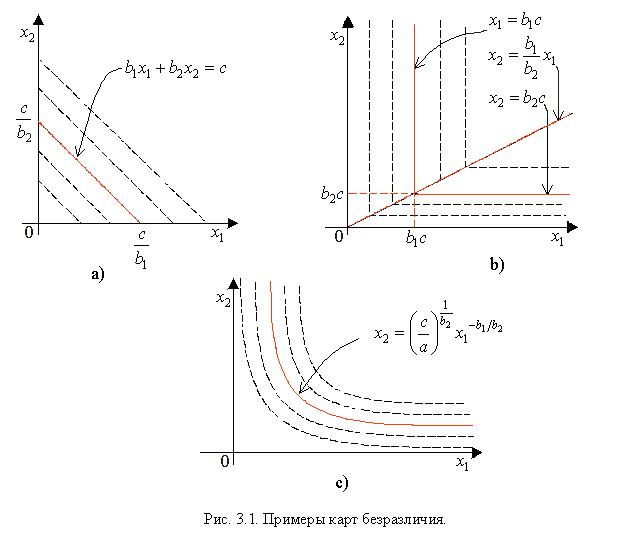
\includegraphics[width=8cm]{31.jpg}}
	\caption{Примеры карт безразличия}
	\label{image2.1}
\end{figure}
\par

Таким образом, функция \eqref{formula3} позволяет определить размер замещения одних товаров другими для того, чтобы полезность оставалась на неизменном уровне.
\par

\textbf{2.} Функция полезности с полным взаимодополнением благ:
\begin{equation}
\label{formula4}
U(x)=min\left\{\frac{x_{i}}{b_{i},i=1,...,n}\right\},
\end{equation}
где $b_{i}$ - количество товара вида \textit{i}, приходящееся на единицу полезности. Для построения кривых безразличия функции \ref{formula4} в $R_{+}^{2}$ из уравнения 
\begin{center}
$min\left\{\frac{x_{1}}{b_{1}}, \frac{x_{2}}{b_{2}}\right\}=c$
\end{center}
\par
Найдём 
\begin{equation}
\label{formula5}
x_{2}=\frac{b_{1}}{b_{2}}x_{1}, \: \text{если} \; \frac{x_{1}}{b_{1}} = \frac{x_{2}}{b_{2}} 
\end{equation}
\begin{equation}
\label{formula6}
x_{1}=b_{1}c, \: \text{если} \; \frac{x_{1}}{b_{1}} < \frac{x_{2}}{b_{2}} 
\end{equation}
\begin{equation}
\label{formula7}
x_{2}=b_{2}c, \: \text{если} \; \frac{x_{1}}{b_{1}} > \frac{x_{2}}{b_{2}}
\end{equation}
\par

Отсюда видно, что карту безразличия функции \ref{formula4} составляют одна линия, проходящая через начало координат и два семейства (по параметру \textit{с}) линий, параллельных осям координат ( рис. \ref{image2.1}.b.)
\par

Функция \ref{formula4} учитывает возможность дополнения одних товаров другими.
\par
\end{example}
\begin{example}
\label{exam2.4}
\rm Приобретается набор из двух товаров: кофе в количестве $x_{1}$ и сахара в количестве $x_{2}$. Потребление этих товаров дает полезность, равную \textit{с}, то есть 
\begin{center}
$U(x)=min\left\{\frac{x_{1}}{b_{1}}, \frac{x_{2}}{b_{2}}\right\}=c$
\end{center}
\par
В случае \ref{formula5} 
\begin{center}
$\frac{x_{1}}{x_{2}}=\frac{x_{2}}{b_{2}}=const$
\end{center}
и увеличение (уменьшение) потребления кофе влечет увеличения (уменьшения) сахара. 
\par
В случае \ref{formula6} увеличение потребления кофе может привести к нарушению неравенства в \ref{formula6} и, следовательно, к нарушению уровня полезности, если не увеличиться потребление сахара.
\end{example}
Анализ случая (\ref{formula7}) предлагается читателю провести самостоятельно.
\par
Как показывает пример \ref{exam2.4}, функция \ref{formula7} применяется для определения полезности набора взаимодополняющих друг друга товаров.

\par
\textbf{3.} Неоклассическая функция полезности (функция Кобба-Дугласа):
\begin{equation}
\label{formula8}
U(x)=\alpha\prod\limits_{i=1}^{n}x_{i}^{b_{i}},b_{1}+b_{2}+,...,b_{n}=1
\end{equation}
где \textit{а} - фактор шкалы измерения полезности, $0<b_{i}<1$. Для построения кривых безразличия функции (\ref{formula8}) в $R_{+}^{2}$ из уравнения $\alpha x_{1}^{b_{1}}x_{2}^{b_{2}}=c$ найдём 

\begin{center}
$x_{2}=\left(\frac{c}{a}\right)^{\left(\frac{1}{b_{2}}\right)}x_{1}^{-\frac{b_{1}}{b_{2}}}$
\end{center}
то есть карту безразличия составляет семейство (по параметру \textit{с}) гипербол, показанных на рис. \ref{image2.1}.с. 
\par
В приведенных примерах функции \ref{formula3} и \ref{formula8} заданы явным образом, а функция \ref{formula4} находится как решение системы неравенств 
$x_{i} \geq b_{i} \: U(x), \: i = 1,2$.
\par
Приведем без комментариев еще несколько видов функции полезности.
\par

\textbf{4.} Функция полезности замещающе-дополняющего типа:
\begin{equation}
\label{formula9}
U(x)=\sum\limits_{i=1}^{n}v_{i}(x)
\end{equation}
где функции находятся из системы неравенств 
\begin{equation}
\label{formula10}
x_{i}\geq \sum\limits_{j=1}^{n}b_{j}v_{j}(x) ,i=1,...,n.
\end{equation}

\par
\textbf{5.} Логарифмическая функция полезности (функция Бернулли):
\begin{equation}
\label{formula11}
U(x)=\sum\limits_{i=1}^{n}a_{i}\log(x_{i}-b{i})
\text{, где} \; a_{i} > 0, x_{i}>b_{i}\geq 0.
\end{equation}

\par
Мы перечислили только некоторые из применяемых в теории потребления функций полезности. Список таких <<готовых>> функций можно продолжить. Однако здесь уместно повторить то, что говорилось ранее о математических моделях в целом - нельзя гарантировать пригодность известных функций для каждого конкретного случая. При моделировании задачи потребителя как раз самым уязвимым местом является функция полезности, адекватно отражающая предпочтения индивидуального потребителя. Поэтому часто требуется не выбрать, а построить для данной конкретной задачи свою функцию полезности. Один из методов приближенного построения функции полезности, использующей понятие предельной нормы замещения.
\par
\begin{center}
\section {Предельный анализ и понятие эластичности в теории потребления}
\end{center}
\par

В экономической теории и практике широко оперируют так называемыми \textit{суммарными} (или абсолютными) и \textit{средними} (или относительными) величинами различных показателей и факторов: объема потребления, дохода, цены товара, спроса, прибыли, производительности труда, издержек, предложения и т.д. Смысл суммарных и средних величин ясен без всякого дополнительного пояснения. Наряду с ними в равной (или даже в большей) степени важны и \textit{предельные величины}.
\par

Насколько возрастает спрос, если предпринять сезонное снижение цен на 10\% ? Как изменится производительность труда фирмы при сокращении рабочего дня на 0,5 часов, а зарплаты на 5\% ? Изменится ли прибыль предприятия (если да, то насколько) при приеме на работу дополнительного рабочего? От какого количества товара одного вида готов отказаться потребитель, чтобы получить одну дополнительную единицу другого товара? Такого рода вопросы, связанные с анализом дополнительного эффекта при дополнительных затратах, возникают во всех сферах экономики. Оперируя только суммарными и средними величинами, нельзя на них ответить. На них можно ответить как раз с помощью предельных величин, определяемых математически с помощью производных соответствующих функций.
\par
Применение в экономике дифференциального исчисления и изучение его результатов называется предельным анализом.Заметим, что дифференциальное исчисление оперирует непрерывно определенными (не дискретными) бесконечно малыми величинами, поэтому приведенные выше термины <<дополнительных единиц>> здесь являются условными.
\par
В этом параграфе речь пойдет о предельных величинах, касающихся только сферы потребления.
\par
Рассмотрим произвольный набор товаров $x\in R_{+}^{n}$. Если полезность от $x_{i}$ обозначить через $U^i(x_{i})$, то суммарная полезность набора \textit{х} есть 
\begin{center}
$U(x)=\sum\limits_{i=1}^{n} U(i)(x_{i})$.
\end{center}
\par
Среднюю полезность набора х схематично можно определить как вектор 
\begin{center}
$\frac{u(x)}{x}=\left(\frac{u^{1}(x_{1})}{x_{1}},...,\frac{u^n(x_{n})}{x_{n}}\right)$
\end{center}
где $\frac{u^i(x_{i})}{x_{i}}$ - средняя полезность товара вида $i$, то есть полезность, приходящаяся на единицу товара $i$.
\par
Понятие предельной полезности набора \textit{х} 
\begin{center}
$\frac{\partial(x)}{\partial x}=\left(\frac{\partial u}{x_{1}},...,\frac{\partial u}{x_{n}}\right)$
\end{center}
мы уже рассматривали в предыдущем параграфе. Вычисляя частное производное $\frac{\partial u}{x_{i}}$, можно получить ответ на вопрос: как себя поведет полезность $U(x)$ при изменении объема потребления того или иного товара. Полезность товара растет, пока справедливо условие \ref{formula}. Если с ростом потребления товара неравенство \ref{formula} переходит в обратное, то очевидно, нет смысла и дальше увеличивать его потребление. Поэтому представляет интерес случай, когда $\frac{\partial u}{x_{i}}=0$. К этому вопросу мы вернемся в следующем параграфе при выявлении оптимальных объемов потребления товара. 
\par
Сравнивая среднюю и предельную полезности, можно обнаружить тенденцию средней полезности <<стремиться>> к предельной полезности. А именно, среднее значение полезности возрастает (при возрастании потребления), если оно ниже предельной полезности; среднее значение полезности остается постоянным (при изменении потребления), если оно равно значению предельной полезности; среднее значение полезности убывает (при возрастании потребления), если оно превосходит предельную полезность.
\par
Сравним среднюю и предельную полезности для разных функций полезности из предыдущего параграфа.
\par
Средняя полезность набора товаров, обладающего свойством замещения \ref{formula3} равна 
\begin{center}
$\frac{u(x)}{x}=\left(\frac{b_{1}x_{1}}{x_{1}},...,\frac{b_{n}x_{n}}{x_{n}}\right)=(b_{1},...,b_{n})$
\end{center}
\par
где $b_{i}$ - средняя полезность товара вида \textit{i}. Предельная полезность есть 
\begin{center}
$\frac{\partial u}{\partial x}=\left(\frac{\partial u}{\partial x_{1}},...,\frac{\partial u}{\partial x_{n}}\right)=(b_{1},...,b_{n})$
\end{center}
\par
Следовательно, для функции \ref{formula3} средняя и предельная полезности совпадают. Этот факт является следствием линейности функции $U$. Подтверждением служит функция полезности для взаимодополняющих друг друга товаров (см. \ref{formula4}): 
\begin{center}
$\frac{u(x)}{x}=min\left\{\frac{1}{b_{1}},...,\frac{1}{b_{n}}\right\},$
\end{center}
\begin{center}
$\frac{\partial u}{\partial x}=min\left\{\frac{1}{b_{1}},...,\frac{1}{b_{n}}\right\},$
\end{center}
\par
Для функции Кобба-Дугласа (\ref{formula8}), полагая для простоты $n=2$, имеем: 
\begin{center}
$\frac{u(x)}{x}=\left( \alpha x_{1}^{b_{1}-1}x_{2}^{b_{2}},\alpha x_{1}^{b_{1}}x_{2}^{b_{2}-1}\right)$
\end{center}
\par
\begin{center}
$\frac{\partial u}{\partial x}=\left(b_{1} \alpha x_{1}^{b_{1}-1}x_{2}^{b_{2}},b_{2} \alpha x_{1}^{b_{1}}x_{2}^{b_{2}-1}\right)$
\end{center}
\par
С учетом условия $b_{1},b_{2}< 1$ ясно, что предельная полезность пропорциональна средней и всегда меньше ее. 
\par
Предельную величину, как и среднюю, можно считать относительной величиной. Пусть значение некоторой переменной \textit{z} изменилась от \textit{z${}_{1}$} до \textit{z${}_{2}$} . Разницу $\Delta z = z_{2}- z_{1} $ называют \textit{абсолютным изменением} \textit{z}, а отношение $\frac{\Delta z}{z_{1}}$ - \textit{относительным изменением} \textit{z} (изменение, приходящееся на одну единицу исходной величины). В отличие от абсолютного относительное изменение есть величина безымянная. Число $\frac{\Delta z}{z_{1}} \times 100\% $ называется \textit{процентным изменением} \textit{z}.
\par
При помощи предельных величин можно формализовать понятие \textit{эластичности}, играющую важную роль при анализе взаимосвязи между экономическими показателями и факторами.
\par
Эластичность (коэффициент эластичности) является численной оценкой относительного изменения экономического показателя под действием относительного изменения некоторого экономического фактора при неизменности других влияющих на этот показатель факторов. Таким образом, эластичность показателя - это его чувствительность к изменению влияющего на него фактора.
\par
Возникает естественный вопрос: зачем нужно вводить сложное понятие <<эластичность>>, когда те же изменения можно описать предельными величинами? Как то: изменение полезности от объема потребления товара $\frac{\partial u}{\partial x_{i}}$, изменение предложения \textit{(y${}_{i}$)} от его цены $\frac{\partial y_i}{\partial p_i}$ - и т.д. Дело в том, что предельные величины, (как и средние) зависят от единицы измерения. Например, величина $\frac{\partial y_i}{\partial p_i}$ в \textit{кг./руб.} есть одно число, а та же величина в \textit{тонна/руб.} - другое. Такая неоднозначность приводит к техническим неудобствам. Эта проблема снимается, если чувствительность экономического показателя измеряется эластичностью, так как последняя определена как безымянная величина.
\par
Пусть имеется некоторый экономический показатель \textit{z}, зависящий от ряда факторов $y_{1},...,y_n$, то есть $z=z(y)=z(y_1,...,y_n)$.Эластичность показателя \textit{z} по \textit{y${}_{i}$} обозначим $\epsilon_{y_{i}}(z)$и выведем общую формулу для ее вычисления.
\par
По определению эластичности
\begin{equation}
\label{formula12}
\epsilon_{y_{i}}(z)=\frac{\frac{\Delta z}{z}}{\frac{\Delta y_i}{y_i}}=\frac{\Delta z }{\Delta y_i} \times \frac{y_i}{z}
\end{equation}
\par

Переходя к пределу в правой части при $\Delta y_i \rightarrow 0$, получим 
\begin{equation}
\label{formula13}
\epsilon_{y_{i}}(z)=\left(\lim\limits_{\Delta y_i \rightarrow 0} \frac{\Delta z}{z}\right){\frac{\Delta y_i}{y_i}}=\frac{\Delta z }{\Delta y_i} \times \frac{y_i}{z}
\end{equation}
\par
Видим, что <<эластичность \textit{z} по \textit{y${}_{i}$}>> вычисляется как произведение <<предельной величины \textit{z} по \textit{y${}_{i}$}>> на <<среднюю величину \textit{y${}_{i}$} по \textit{z}>>. 
Умножая числитель и знаменатель дроби \ref{formula11} на 100\%, получим
\begin{equation}
 \epsilon_{y_{i}}(z)=\frac{\frac{\Delta z}{z}\times 100\%} {\frac{\Delta y_i}{y_i}\times 100\%}
 \label{formula14}
\end{equation}
\par
Отсюда, эластичность \textit{z} по \textit{y${}_{i}$} есть отношение процентного изменения \textit{z} на процентное изменение \textit{y${}_{i}$}. 
\par
Интересно узнать, насколько процентов изменится \textit{z} , если \textit{y${}_{i}$} изменится на 1\%? Иначе говоря, нужно найти процентное изменение \textit{z} при процентном изменении \textit{y${}_{i}$} , равном единице, то есть 
$\frac{\Delta y_i}{y_i}100\%=1$ Тогда из \ref{formula13} сразу получаем искомое процентное изменение:
\begin{center}
$\frac{\Delta z_i}{z_i}100\%=\epsilon_{y_{i}}(x)|_{1\%}$.
\end{center}
\par
Отсюда, эластичность \textit{z} по \textit{y${}_{i}$} есть процентное изменение показателя \textit{z} при изменении фактора \textit{y${}_{i}$} на 1\%. 
\par
Как видно из (\ref{formula12}), знак эластичности в каждой точке \textit{y} зависит от знаков $\frac{\partial z}{\partial y_i}$ и $\frac{y_i}{z}$. Предположим для простоты, что $\frac{y_i}{z}>0 $. Тогда, если \textit{z} возрастает по \textit{y${}_{i}$} (в точке \textit{y} ), тогда $\frac{\partial z}{\partial y_i} > 0 $ и эластичность положительна; если \textit{z} убывает по \textit{y${}_{i}$} , тогда $\frac{\partial z}{\partial y_i}< 0 $ и эластичность отрицательна. В этом смысле представляет интерес случай, когда $\frac{\partial z}{\partial y_i} = 0 $, анализ которого и его содержательную интерпретацию мы оставим читателю.
\par
Пороговым значением для эластичности является число 1. Для объяснения этого рассмотрим графическое изображение эластичности функции спроса \textit{(с)} на один товар, зависящей только от его цены: \textit{c=c(p)}. Известно, что спрос является убывающей функцией цены. Вычислим эластичность $\epsilon_p(c)$ в произвольной точке \textit{A(p,c)} графика функции \textit{c=c(p)} ( рис. \ref{image2.2} ).
\par
\begin{figure}[h]
	\center{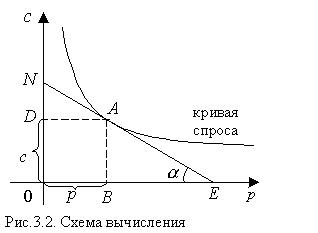
\includegraphics[width=8cm]{32.JPG}}
	\caption{Схема вычисления}
	\label{image2.2}	
\end{figure}
Пресечение касательной в точке \textit{А} с осями координат обозначим через \textit{Е} и \textit{N}. По определению
\begin{center}
$\epsilon_p(c)=\frac{dc}{dp}\frac{p}{c}$.
\end{center}
\par

Выразим правую часть равенства через элементы графика. Из $\tg \alpha = \frac{AB}{BE}$ имеем
\begin{center}
BE=$\frac{AB}{\tg \alpha }=\frac{OD}{\tg \alpha }=\frac{c}{-\frac{dc}{dp}}=$
\end{center}
здесь знак минус показывает убывание функции \textit{с} в точке \textit{А}). Из подобия треугольников \textit{ABE} и \textit{ADN} имеем: 
\begin{center}
$\frac{AN}{AE}=\frac{AD}{BE}=\frac{OB}{BE}=\frac{p}{\frac{-c}{\frac{dc}{dp}}}=-\frac{dc}{dp}\frac{c}{p}=-\epsilon_p(c)$
\end{center}
\par

Следовательно, 
\begin{equation}
\label{formula15}
\epsilon_p(c)=-\frac{AN}{AE}.
\end{equation}

\par
Можно показать, что для возрастающей функции (например, предложения, как функции от цены) эластичность по абсолютной величине также будет равна отношению \textit{AN/AE}. Потому в общем случае эластичность следует оценивать по ее абсолютной величине. Эта величина равна 1, если в (\ref{formula14}) числитель равен знаменателю; больше 1, если числитель больше знаменателя и меньше 1 - если числитель меньше знаменателя. Это говорит о том, что эластичность $\epsilon_{y_{i}}(z)$ зависит от кривизны графика функции \textit{z} в рассматриваемой точке.

\par
Если $\left|\epsilon_{y_{i}}(z)\right|>1$, то функция \textit{z} называется эластичной (по \textit{y${}_{i}$}); если $\left|\epsilon_{y_{i}}(z)\right|<1$, то функция \textit{z} называется неэластичной (по \textit{y${}_{i}$}); если $\left|\epsilon_{y_{i}}(z)\right|=1$, то говорят, что функция \textit{z} имеет единичную эластичность (по \textit{y${}_{i}$}).

\par
Относительно спроса различают товары эластичного спроса и товары неэластичного спроса. Для товаров первого вида повышению цены на 1\% соответствует понижение спроса более, чем на 1\% и, наоборот, понижение цены на 1\% приводит к росту покупок более, чем на 1\% $\left(\left|\epsilon_{p}(c)\right|>1\right)$. Для товаров второго вида повышение цены на 1\% влечет за собой понижение спроса менее, чем на 1\% и, наоборот, уменьшение цены на 1\% приводит к росту покупок менее чем на 1\% $\left(\left|\epsilon_{p}(c)\right|<1 \right)$. К этому вопросу мы еще раз вернемся после формализации понятия спроса.

\par
Вычислим эластичность некоторых из функций полезности, для простоты будем полагать $n=2$.

\begin{center}
$\epsilon_{x_{i}}(u)=\frac{\partial u }{\partial x_i}\frac{x_i}{u}=\frac{b_i x_i}{b_1 x_1 + b_2 x_2},i=1,2$
\end{center}

\par
Например, в точке $\vec{x}=\left(\frac{1}{b_1},\frac{2}{b_2}\right)$ получаем:

\begin{center}
$\epsilon_{x_{1}}(u)|_{x_{1}=x_{1}}=\frac{1}{3}, \epsilon_{x_{2}}(u)|_{x_{2}=x_{2}}=\frac{2}{3}$
\end{center}

\par
Видим, что в точке $\overline{x}$ полезность в целом неэластична; при этом неэластичность по второму товару <<выше>>, чем по первому товару. Более детальный анализ эластичности функции (\ref{formula3}) оставляем читателю.
 
\par
Для функции Кобба-Дугласа (\ref{formula8}) имеем: 
\begin{center}
$\epsilon_{x_1}(u)=b_1 \alpha x_{1}^{b_{1}-1}x_{2}^{b_2} \frac{x_1}{\alpha x_{1}^{b_{1}}x_{2}^{b_2}}=b_1$
\end{center}
\begin{center}
$\epsilon_{x_2}(u)=b_2 \alpha x_{1}^{b_{1}}x_{2}^{b_{2}-1} \frac{x_2}{\alpha x_{1}^{b_{1}}x_{2}^{b_2}}=b_2$
\end{center}
\par

Итак, параметры $b_1$ и $b_2$ в функции Кобба-Дугласа как раз являются коэффициентами эластичности по видам товаров; они постоянны, то есть не зависят от объема потребления. Поэтому функция Кобба-Дугласа относится к классу функций полезности с постоянной эластичностью (вернее, неэластичностью, так как $b_{1},b_{2}<1$).

\begin{figure}[h]
	\center{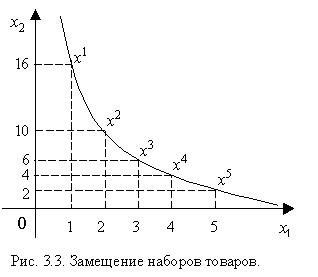
\includegraphics[width=8cm]{33.JPG}}
	\caption{Замещение наборов товаров}
	\label{image2.3}
\end{figure}

\par
В завершение параграфа рассмотрим еще одно понятие, определяемое с помощью дифференцирования.

\par
Предположим, что имеется шесть наборов товаров 
\begin{center}
$x^1=(1,16), \: x^2=(2,10),\: x^3=(3,6),\: x^4=(4,4),\: x^5=(5,2)$
\end{center}
с одинаковой полезности, то есть $U(x^1)=...=U(x^5)$. Пусть первый вид товара \textit{(i=1)} - продукт питания, второй \textit{(i=2)} - одежда. Эти точки лежат на одной кривой безразличия \textit{u(x)=c} (рис. \ref{image2.3}). Как видно из графика, замена набора $x^1$ набором $x^2$ требует отказа от 6 единиц одежды взамен на одну единицу продукта питания; замена $x^2$ на $x^3$ - отказа от 4 единиц одежды ради одной единицы продукта питания и т.д. Чтобы количественно определить объем некоторого товара, которым потребитель готов пожертвовать ради другого товара, используют меру, называемую предельной нормой замещения. Более точно, предельная норма замещения показывает, на сколько единиц нужно уменьшить (увеличить) количество одного товара при увеличении (уменьшении) другого товара на единицу, чтобы при этом полезность осталась неизменной.
 
\par
Обозначим предельную норму замещения i-го товара j-м товаром через $S_{ij}$ и выведем формулу для ее вычисления.

\par
Пусть при уменьшении потребления \textit{j}-го товара на величину $\Delta x_j$ для поддержания прежнего уровня полезности необходимо увеличить потребление \textit{i}-го товара на величину $\Delta x_i$:
 
\begin{equation}
\label{formula16}
U(x_1, \dots, x_n)=U(x_1, \dots , x_i+d x_i, \dots, x_j+d x_j, \dots, x_n)
\end{equation}
где $d x_i= \Delta x_i,\; d x_j=-\Delta x_j$. По определению предельной нормы замещения
\begin{equation}
\label{formula17}
S_{ij}=\frac{\Delta x_j}{\Delta x_i}|_{U=const}
\end{equation}

\par
Из (\ref{formula16}) получаем
\begin{equation}
\label{formula18}
\Delta U = U(x_1, \dots, x_i+d x_i, \dots ,x_j+ d x_j, \dots, x_n)-U(x_1, \dots, x_n)=0
\end{equation}

Для полного приращения $\Delta U$ функции \textit{U} в математическом анализе существует формула:
\begin{equation}
\label{formula19}
\Delta U = \frac{\partial U}{\partial x_1}d x_1 + \dots + \frac{\partial U} {\partial x_n} + \epsilon (\Delta x_1, \dots, \Delta x_n),
\end{equation}
где $\epsilon > 0 $ таково, что

\begin{equation}
\label{formuala20}
\lim\limits_{\Delta x_i \rightarrow 0} \epsilon (\Delta x_1, \dots,\Delta x_n)=0
\end{equation}
есть полный дифференциал функции \textit{U}. Из (\ref{formula18})-(\ref{formuala20}) с учетом того, что $d x_k =0 $ для $k \neq i,j$, имеем 
\begin{equation*}
dU= \frac{\partial U}{\partial x_i} d x_i + \frac{\partial U}{\partial x_j}d x_j =0
\end{equation*}
Отсюда 
\begin{center}
$\frac{\frac{\partial U}{\partial x_i}}{\frac{\partial U}{\partial x_j}}= -\frac{d x_j}{d x_i}=\frac{\Delta x_j}{\Delta x_i}$
\end{center}
и из (\ref{formula17}) получаем окончательно 

\begin{equation}
\label{formuala21}
S_{ij}=\frac{\frac{\partial U}{\partial x_j}}{\frac{\partial U}{d x_j}}
\end{equation}

Следовательно, предельная норма замещения товаров выражается через отношение их предельных полезностей. Например, для функции Кобба-Дугласа (2.8) имеем: 
\begin{center}
$S_{ij}=\frac{b_i}{b_j}\frac{x_j}{x_i}, i,j=1,...,n (i \neq j)$
\end{center}
\par

Из закона об убывающей предельной полезности следует выпуклость кривых безразличия. Поэтому при движении вниз вдоль кривой безразличия ( рис. 3.3 ) $S_{12}$ убывает:
\begin{center}
$S_{12}(x^1) = 6,S_{12}(x^2)=4, S_{12}(x^3)= 2, S_{12}(x^4)= 1 $
\end{center}

Этот факт в экономике называется законом убывающей предельной нормы замещения: при стремлении поддерживать неизменным уровень полезности путем замещения \textit{i-го} товара \textit{j-м} товаром, субъективное удовлетворение, получаемое от предельного потребления \textit{i-го} товара, в сравнении с удовлетворением, получаемым от предельного потребления товара \textit{j}, будет неуклонно уменьшаться. 
\par

Формы кривых безразличия показывают на разные степени желательности замены одного товара другим. Пусть кривые безразличия для двух различных потребителей относительно напитка \textit{(i=1)} и сока (\textit{i=2)} имеют следующий вид (рис. \ref{image2.4} и рис. \ref{image2.5}): 
\par
\begin{figure}[h]
	\begin{minipage}[h]{0.49\linewidth}
		\center{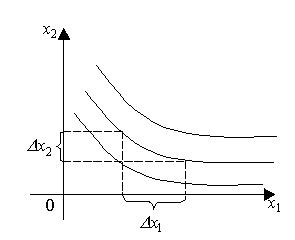
\includegraphics[width=0.9\linewidth]{34.jpg} \\}
		\caption{Предпочтение первого потребителя.} %% подпись к рисунку
		\label{image2.4} %% метка рисунка для ссылки на него
	\end{minipage}
	\hfill
	\begin{minipage}[h]{0.49\linewidth}
		\center{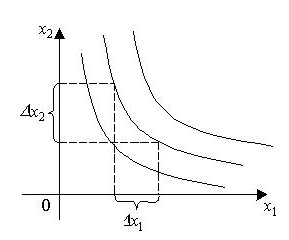
\includegraphics[width=0.9\linewidth]{34_1.jpg} \\}
		\caption{Предпочтение второго потребителя} %% подпись к рисунку
		\label{image2.5} %% метка рисунка для ссылки на него
	\end{minipage}
	
\end{figure}
У первого потребителя (рис. \ref{image2.4}) низкая предельная норма замещения напитка соком - он готов отказаться от очень небольшого количества сока ради напитка ($\Delta x_2 < \Delta x_1$). У второго потребителя (рис. \ref{image2.5}), наоборот, высокая предельная норма замещения напитка соком ($\Delta x_2 > \Delta x_1$).
\par

Предельная норма замещения применяется при изучении спроса (напр., что нужнее в данный момент для домашнего хозяйства, один диван или два кресла; насколько нужно жертвовать технической характеристикой автомобиля ради увеличения комфорта и т.д.). Формализацию понятия спроса, изучению его природы и свойств посвящены следующие параграфы этой главы.
\newpage


\begin{center}
\section {Оптимизационная модель задачи потребительского выбора}
\end{center}
\par

В этом параграфе мы приведем и исследуем классическую математическую модель задачи индивидуального потребительского выбора. Содержательно эту задачу можно сформулировать так: потребителю нужно приобрести (купить) на рынке необходимые ему виды товаров в таком количестве, чтобы их потребление доставило максимальное удовлетворение (пользу); при этом суммарная стоимость купленных товаров не должна превышать его дохода (бюджета).

Последнее условие называется бюджетным ограничением и оно подчеркивает всегда ограниченные покупательские возможности потребителя. 
\par

Обращает на себя внимание <<скудность>> постановки задачи. Так, например, не говорится о минимальном прожиточном уровне, ниже которого объем потребления не может опускаться; нет ограничения на доход потребителя и т.д. Однако , следует исходить из того, что эта постановка общая и в случае необходимости более подробного моделирования все недостающие сведения можно <<прочитать между строчками>> этой постановки. Мы же будем принимать эту постановку как исходную, ее и будем моделировать.
\par

В начале {§ \ref{par2.1}} мы перечислили те важнейшие факторы, которые будучи формализованы и связаны подходящими математическими соотношениями и дают требуемую модель. Это товар и его цена, цель и бюджет потребителя, его покупательская способность. 
\par
 
Приведем сначала необходимые обозначения, хотя некоторые из них уже были введены в §§ 3.1 , 3.2.
\par

Пусть $x = (x_1,...,x_n)\in R_{+}^{n}$ - набор товаров, где $x_i$ - количество товаров вида \textit{i,n} - число видов товаров, $R_{+}^{n}$ - пространство товаров; $p=(p_1,...,p_n)$ - вектор цен товаров, где $p_i$- цена единицы товара вида \textit{i};\textit{K}-доход (бюджет) потребителя.
\par

Мы рассматриваем статическую задачу, поэтому эти величины не зависят от фактора времени. Параметры $p_i$ и \textit{K} считаются постоянными величинами, причем цены считаются рыночными, а доход не структуризуется, то есть нас не интересует из каких частей он складывается. Компоненты \textit{xi} вектора являются неизвестными переменными. Модель составляется как раз для определения <<оптимальных>> значений этих переменных для данного потребителя. Цель потребителя будем описывать с помощью функции полезности 
$U:R_{+}^{n} \rightarrow R^1$ (см.  § 3.2 и определение 3.1), относительно которой будем предполагать выполнение условий (2.1) и (2.2) . Наконец, мы рассматриваем некоторого <<обобщенного>> потребителя, никак не характеризуя его индивидуальные особенности, за исключением априорного предложения о существовании функции полезности, отражающей его индивидуальные предпочтения в $R_{+}^{n}$ (см. Теорему 3.1 ).
\par

С учетом всего сказанного выше, модель задачи потребительского выбора имеет вид:
\begin{center}
$U(x) \rightarrow max$ (4.1)
\end{center}
\par
при ограничениях 
\begin{center}
$\left\langle p,x \right\rangle \leq K$,
\end{center}
\begin{center} 
$x \geq 0$ (4.2)
\end{center}
\par

Обозначим через  \textit{B(p,K)}множество всевозможных товаров, допустимых потребителю при ценах \textit{p} и доходе \textit{K}:
\begin{center}
$B(p,K) =  \left\{ x \in R_{+}^{n}| \left\langle p,x \right\rangle \leq K \right\}$ (4.3)
\end{center}
называемое бюджетным множеством. Графическое изображение этого множества показано на рис.3.6. 
\par

Граница $\overline{B}(p,K) =  \left\{ x \in R_{+}^{n}| \left\langle p,x \right\rangle = K \right\} $ множество $B(p,K)$ называется бюджетной линией.
\par

Оптимальным решением задачи (4.1)-(4.2) называется такой вектор $x^{*} =(x_{1}^{*},...,x_{n}^{*})$ , что 
\begin{center}
$U(x^{*})= \max \limits_{x \in B(p,k)}  U(x)$ (4.4)
\end{center}
\par

\textbf{Определение 3.3.} Оптимальное решение $x^{*}$ задачи (4.1) - (4.2) называется спросом потребителя. 
\par

Данное формальное определение спроса отражает классическое понятие спроса как платежеспособную потребность. 
\par

Всегда ли существует оптимальное решение задачи (4.1) - (4.2) ?
\par

Поскольку мы имеем дело с оптимизационной задачей (линейной или нет в зависимости от функции полезности \textit{U} ) (см. § 2.3 ), то на этот вопрос следует ответить с точки зрения теоремы Вейерштрасса. Так как функция полезности непрерывна по факту ее существования (см. Теорему 2.1 ), основная сложность заключается в компактности множества (4.3) , на котором ищется максимум функции \textit{U} (см. (4.4)). В метрическом пространстве  $R_{+}^{n}$, как известно, компактность множества равнозначно его замкнутости и ограниченности. Так как бюджетное множество замкнуто по определению, то остается изучить его ограниченность.
\par

Покажем, что ограниченность не всегда имеет место. Предположим, для некоторого $i p_i=0$ . Как следует из (4.2) , в этом случае <<допустимым>> становится любой вектор $\widetilde{x}=x_1,...,x_{n-1},\infty, x_{i+1},...,x_n)$, то есть $\widetilde{x} \in B(p,K)$ , что говорит о неограниченности бюджетного множества. А это, в свою очередь, может привести к отсутствию оптимального решения задачи (4.1)-(4.2) (напр., в случае неограниченности функции \textit{U}, что является следствием ненасыщаемости потребителя (см. свойство a'5 в §3.2 )). Однако, если потребитель ненасыщаем по всем товарам, то множество  \textit{B(p,k)} оказывается ограниченным. Более строже этот факт сформулирован в следующем утверждении.
\par

\textbf{Теорема 3.3.} Пусть бюджетное множество (4.3) обладает следующим свойством: если в последовательности $x^{k} \in B(p,K)$ при $k \rightarrow \infty$ имеет место $x_{i}^{k} \rightarrow \infty $ для некоторого \textit{j} , то  для всех \textit{i=1,...,n}. Тогда бюджетное множество ограничено и в задаче (4.1)-(4.2) существует оптимальное решение. Если при этом функция u строго вогнута на множестве  , то оптимальное решение единственно.
\par

Итак, при фиксированных ценах $p_1,...,p_n$ и заданном доходе \textit{K} оптимальное потребление определяется компонентами $x_{1}^{*},...,x_{n}^{*}$ решения  задачи $x^{*}$(4.1)-(4.2).
\par

Выяснив существование оптимального решения задачи потребителя, займемся вопросом его вычисления. Для этого воспользуемся методом множителей Лагранжа.
\par

Составим функцию Лагранжа для нашей задачи: 
\begin{center}
$L(x,\lambda , \mu )= U(x) + \lambda (K- \left\langle p,x \right\rangle)+\mu x$
\end{center}
\par
где $\lambda , \mu $ множители Лагранжа. Выпишем необходимые условия оптимальности (условия Куна-Таккера),которые благодаря условиям (2.2) будут и достаточными: 
\begin{center}
$$\left\{
\begin{aligned}
\frac{\partial u}{\partial x} - \lambda p + \mu & = 0,\\
\lambda (K- \left\langle  p, x \right\rangle) & = 0,\\
\mu x = & 0\\
(K- \left\langle  p, x \right\rangle) & = 0 \\
x \geq 0,\lambda \geq 0,\mu \geq & 0
\end{aligned}
\right.$$
\end{center}
\par

Не умаляя общности рассуждений, примем следующее предложение: потребитель приобретает все виды товаров, то есть $x_i>0$ для всех \textit{i=1,...,n }(в противном случае можно уменьшить размерность пространства $R_{+}^{n}$ ) и будем считать, что $p_i>0,i=1,...,n$ . Тогда из третьего равенства следует $\mu =0$ и необходимые и достаточные условия принимают вид: 
\begin{center}
$\frac{\partial U}{\partial x } - \lambda p =0, (4.5)$
\end{center}
\begin{center}
$\lambda(K - \left\langle p,x\right\rangle)=0$ (4.6)
\end{center}
\begin{center}
$K - \left\langle p,x\right\rangle \geq 0$ (4.7)
\end{center}
\begin{center}
$x \geq 0, \lambda > 0$ (4.8)
\end{center}
\par

Эта система разрешима относительно \textit{n+1} неизвестных $x_1,...,x_n, \lambda$ , так как имеется \textit{n+1} уравнение (4.5) и (4.6). Все переменные и частные производные здесь вычисляются в точке  $x^{*}$. Значение $\lambda$ соответствующее (в силу уравнений (4.5) и (4.6)) точке $x^{*}$ обозначим  $\lambda^{*}$.
\par

Для пары ($x^{*}$ , $\lambda^{*}$ ) из (4.5) получаем: 
\begin{center}
$\frac{1}{p_1} \frac{\partial u}{\partial x_1}=\frac{1}{p_2}\frac{\partial u}{\partial x_2}= ... = \frac{1}{p_n}\frac{\partial u}{\partial x_n}$
\end{center}
\par
означает, что предельная полезность одной единицы денег одинаково для каждого товара и именно при таком распределении бюджета потребитель получает максимум полезности. Для объяснения этого факта обратимся к рис. 3.3. Если полезность от расходования дополнительного доллара на продукт питания выше, чем от доллара на одежду, то потребитель может увеличить полезность за счет роста расходов на питание. Таким образом, увеличение расходов на питание вызовет уменьшение расходов на одежду и это будет продолжаться до тех пор, пока предельная полезность на питание будет выше чем на одежду. По закону Госсена предельная полезность продуктов питания постепенно снизится, вызывая рост расходов на одежду. Только тогда, когда предельная полезность дополнительного доллара расходов становится одинаковой для питания и одежды, будет достигнут максимум полезности.
\par

Из равенства (4.9) следует так же вывод о том, что цены должны определяться исходя из предельной полезности товаров и денег: 
\begin{center}
$p_i=\frac{1}{\lambda^{*}}\frac{\partial \partial u}{\partial x_i}|_{x=x^{*}}, i = 1,...,n$
\end{center}
\begin{center}
Так как $\lambda^{*}>0$(следует из (4.5) ), то из (4.6) получаем 
\end{center}
\begin{center}
$K - \left\langle p,x^{*}\right\rangle = 0$.
\end{center}
\par

Последнее означает, что точка максимума $x^{*}$ задачи (4.1) - (4.2) лежит на бюджетной линии. В случае двух товаров имеем (см. рис 3.7 ): 
\begin{center}
$$\left\{
\begin{aligned}
\frac{\partial u}{\partial x_1}(x_1,x_2)+\lambda p_1 & = 0,\\
\frac{\partial u}{\partial x_2}(x_1,x_2)+\lambda p_2 & = 0,\\
K-p_1 x_1 - p_2 x_2 = 0. 
\end{aligned}
\right.$$
\end{center}
\par

Наклон бюджетной линии равен 
\begin{center}
$\tg \alpha = - \frac{\frac{K}{p_2}}{\frac{K}{p_1}}=-\frac{p_1}{p_2}$
\end{center}
\par

Наклон кривой безразличия $U (x_1,x_2)= const$ находится из выражения $dU=0$ , то есть
\begin{center}
$\frac{\partial u}{\partial x_1}dx_1 + \frac{\partial u}{\partial x_2}d x_2=0$
\end{center}
\par

и составляет
\begin{center}
$\frac{dx_2}{dx_1}= - \frac{\frac{\partial u}{\partial x_1}}{\frac{\partial u}{\partial x_2}}$
\end{center}
\par

Так как в точке касания $x^{*}$ наклон кривой безразличия равен наклону бюджетной линии, то 
\begin{center}
$\frac{d x_2}{d x_1}= -\frac{p_1}{p_2}$
\end{center}
или 
\begin{center}
$\frac{\frac{\partial U}{\partial x_1}}{\frac{\partial U}{\partial x_2}}=\frac{p_1}{p_2}$ (4.10)
\end{center}
\par

Как видно из (4.9), и в частности, из (4.10),
\begin{center}
$S_{i,j}|_{x=x^{*}}=\frac{p_i}{p_j}, i,j = 1,...,n,$
\end{center}
\par

то есть в оптимальном наборе товаров $x^{*}=(x_{1}^{*},...,x_{n}^{*})$ предельная норма замещения товара \textit{i} товаром \textit{j} оценивается отношением их цен (то есть зависит исключительно от их цен). 
\par

Как показывает рис. 3.7, оптимальное решение задачи (4.1)-(4.2) геометрически является точкой касания кривой безразличия и бюджетной линии. Для строго вогнутой функции полезности такая точка касания единственна (см. Теорему 3.3).
\par

С помощью рис. 3.7 можно анализировать различные последствия, связанные с изменением цен и дохода.
\par

Будем считать, что все товары нормальные (качественные), то есть при увеличении дохода потребление увеличивается. Нас интересуют следующие вопросы: 
\par

а) изменение покупательской способности: как изменится спрос на товары при изменении их цен и неизменном доходе? 
\par

б) эффект замещения: как изменится потребление товаров, когда при изменении цен полезность должна оставаться на прежнем уровне? 
\par

в) эффект дохода: как изменится потребление товаров при изменении дохода потребителя и неизменных ценах?
\par

Обсудим случай а) . Предположим, что снижается цена первого товара. Тогда бюджетная линия из положения \textit{АВ} переходит в положение \textit{АС} ( рис. 3.8 ). 
\par

Так как кривые безразличия заполняют все пространство $R_{+}^{2}$, то обязательно найдется одна кривая безразличия, имеющая с бюджетной линией \textit{АС} точку касания. Обозначим эту точку $x^{**}$ . Она и будет оптимальным решением задачи потребителя при новых ценах. В точке $x^{**}$  полезность будет больше чем в точке $x^{*}$, за счет увеличения на величину $x_{1}^{**}-x_{1}^{*} > 0$  потребления первого товара. Это стало возможным в результате роста покупательской способности потребителя (его реального дохода), благодаря снижению цены на первый товар. Что произошло при этом с объемом потребления второго товара? Он снизился на велечину $x_{1}^{**}-x_{1}^{*} > 0$.Здесь отражена та реальность, когда люди потребляют большее количество (качественного) товара, который подешевел, и меньшее количество тех товаров, которые остались на прежнем ценовом уровне или подорожали.
\par

Читателю предлагается самостоятельно анализировать случаи уменьшения цены товара и одновременного изменения цен на оба вида товара. 
\par

Рассмотрим эффект замещения (случай б)). Предположим опять, что первый продукт стал более дешевым (по сравнению с тем, что было в точке $x^{*}$). Так как при этом полезность не должна меняться, то эффект замещения отражается смещением точки $x^{*}$ вдоль кривой безразличия $U=U(x^{*})$ , то есть новое оптимальное решение $\overline{x^{*}}$ задачи потребителя будет находится на одной кривой безразличия с точкой $x^{*}$ ( рис. 3.8 ). Бюджетная линия \textit{A'C'} , касающаяся кривой безразличия $U=U(x^{*})$ в точке $\overline{x^{*}}$, параллельна изменившейся бюджетной линии \textit{АС} и удалена от нее на величину изменения реального дохода (покупательской способности). Следовательно, эффект замещения представляется величиной $\overline{x_{1}^{*}} - x_{1}^{*}$.
\par

Проверив эффект дохода ( случай в )) самостоятельно убедитесь, что он характеризуется ростом потребления первого товара на величину $\overline{x_{1}^{*}} - x_{1}^{*}$ .
\par

Мы видим, что пользуясь решением задачи (4.1) - (4.2 ) можно анализировать различные ситуации и ответить на многие вопросы, круг и глубина которых зависит от творческих способностей исследователя.
\par

В зависимости от условий конкретной задачи, свойств товаров и прочего в выражении (4.1) можно либо использовать одну из известных функций полезности, например, одну из функций (2.3) , (2.4) , (2.8) - (2.12) , либо построить новую функцию полезности.
\par

Надо заметить, что в теории потребления нет общих или универсальных методов построения функций полезности. Известныо лишь частные методы для некоторых отдельных классов таких функций. Приведем один способ приближенного построения так называемых аддитивных функций полезности. Такие функции применяются в тех случаях, когда полезность набора товаров $x = (x_1,...,x_n) \in R_{+}^{n}$ складывается как сумма полезностей товаров отдельных видов: 
\begin{center}
$U(x)=\sum\limits_{i=1}^{n} U_{i}(x_{i})$ (4.11)
\end{center}
\par

Будем считать, что функция (4.11) задана на \textit{n-мерном} параллелепипеде: 
\begin{center}
$a_i \leq x_i \leq b_i (b_i > a_i) i=1,...,n$
\end{center}
\par

Обозначим $X_i=[a_i,b_i]$. Тогда пространство товаров имеет вид: 
\begin{center}
$X = \prod \limits_{i=1}^{n}X_i = X_1 \cdot ... X_n.$ 
\end{center}
(это и есть n-мерный параллелепипед). 
\par

Идеи метода заключаются в построении линий безразличия на каждом из \textit{n-1} граней параллелепипеда X . Исходной информацией для этого является определяемость линий безразличия условиями замещения товаров (см. рис. 3.3 ).
\par

Алгоритм метода следующий. 
\par

1.	Выявление взаимозаменяемых товаров: в общем случае товары вида i0 и j0 будут взаимозаменяемыми, если существует последовательность взаимозаменяемых пар 
\begin{center}
$\left\{(i_0,j_1),(j_1,j_2),...,(j_k,j_0)\right\}$
\end{center}
\par

2.	Вычисление предельных норм замещения: для каждой пары (\textit{i,j)} из (3.4.12) вычисляют величину $S_{ij}$ по формуле (3.9) или (3.5) . 
\par

3.	Построение кривых безразличия на гранях параллелепипеда \textit{Х}: с помощью чисел $S_{ij}$, полученных в п.2, сроят по одной линии безразличия в прямоугольниках $X_i \times X_j$(см. рис. 3.3 ). 
\par

4.	Разбиение граней одного из прямоугольников $X_i \times X_j$ точками: выбирают один из прямоугольников, например,$X_1 \times X_2 $  и для кривой безразличия строят ее близкое смещение (то есть новую кривую безразличия) (см. рис. 3.9 ); разбиение отрезков $Х_1$ и $Х_2$ получают с помощью <<лестницы>> между двумя кривыми безразличия. 
\par

5.Построение функции полезности для товара \textit{i=1} : для полученного в п.4 разбиения отрезка $X_1$ строят функцию полезности $U_1(x_1)$ предполагая, что на каждом интервале разбиения функция $U_1$ возрастает на одну единицу ( рис. 3.10 ). 
\par

6.	Последовательное разбиение остальных отрезков $X_i$ : эту процедуру проводят индуктивно, как показано на рис. 3.11. 
\par

7.	Последовательное построение функции полезности для остальных товаров: для получения в п.6. последовательных разбиений отрезков $X_i$ строят функции полезности $U_i(x_i)$ как в п.5. 
\par

8.	Построение общей функции полезности: после того, как получены все $U_i$, \textit{i=1,...,n} , полагают $U(x)= U_1(x_1)+ ... U_n(x_n)$ . 
\par

Заметим, что точность аппроксимации функции полезности \textit{U} зависит от близости исходной и смещенной кривых безразличия в п.4.
\newpage
\begin{center}
\section {Функция спроса и ее свойства}
\end{center}
\par

В предыдущем параграфе спрос был определен как оптимальное решение $x^{*}$ задачи потребителя (4.1) - (4.2) (см. определение 3.3 ). Спрос есть платежеспособная потребность, а платежеспособность предполагает соответствие цен и дохода. Поэтому мы можем утверждать, что общее решение задачи потребителя вычисляется как функция от цен и дохода :$x^{*} = x^{*} (p,K)$ . Точно так же  $\lambda ^{*} = \lambda ^ {*}(p,K)$. К этому же выводу можно прийти исходя из вида задачи (4.1) - (4.2) , так как \textit{p} и \textit{K} являются параметрами этой задачи.
\par

Решение оптимизационной задачи - это лишь один из способов определения спроса, который схематично можно представить так: 
\begin{center}
$(p,K)\stackrel{D}{\rightarrow} x^{*}(p,K),$
\end{center}
где \textit{D}- отображение, представленное максимизацией функции \textit{U} с учетом бюджетного ограничения. В общем случае \textit{D} - это некоторая совокупность правил, с помощью которых потребитель определяет свой спрос. 
\par

Пусть $X \subset R_{+}^{n}$ - множество допустимых наборов товаров, $P \subset R_{+}^{n}$ - пространство цен. Функцией спроса (индивидуального потребителя) называется отображение \textit{D} , которое каждой паре $(p,K) \in P \times R_{+}^1$ ставит в соответствие множество наиболее предпочтительных наборов товаров 
\begin{center}
$D:P \times R_{+}^{n} \rightarrow 2^X,$(5.1)
\end{center}
где $2^X$ - множество всех подмножеств множества \textit{X} . Это же отображение можно записать как
\begin{center}
$(p,K) \rightarrow D(p,K) \subset X$.
\end{center}
\par

Любая точка $x^{*}\in D(p,K)$ называется спросом (при ценах \textit{p} и доходе \textit{K}). 
\par

Итак, в общем случае функция спроса - это многозначное отображение. Действительно, если  $x^{*}$ - вектор спроса, а множество $D^{*} = \left\{y \in X : y \sim x^{*} \right\}$ не пусто, то любая точка множества $D^{*}$ является спросом.
\par

Для отображения \textit{D}, представленного задачей (4.1) - (4.2) , имеем: 
$$ D(p,K)= \left\{
\begin{aligned}
\left\{ x^{*} \in B(p,K):U(x^{*}) = \max\limits_{x \in B(p,K)} U(x) \right\},\text {если максимум достигается}\\
\oslash , \text {если максимум не достигается.}
\end{aligned}
\right.$$
\par

Если в (4.1) функция полезности \textit{U} строго вогнута, то функция спроса \textit{D} однозначна, т.е. множество $D(p,k)$ состоит из одной точки $x^{*}$ максимума функции $U:x^{*} = D(p,K)$. 
\par

В случае неоднозначности функции спроса возникает дополнительная проблема выбора единственной точки $x^{*} \in D(p,K)$. Этот вопрос будет рассмотрен в главе далее. 
\par

Принимая во внимание тот факт, что доход потребителя зависит от цен товаров, можно в пространстве $P\subset R_{+}^{n} $ определить функцию спроса $\widetilde{D}:p \rightarrow 2^{X}$ , так что $\widetilde{D}(p) = D(p,K(p)) $.
\par

При увеличении цен на товары, вообще говоря, доход потребителя должен быть компенсирован. Это требование формализуется как свойство однородности первой степени (или линейной однородности) функции дохода: для любых $a \geq 0 K(\alpha \cdot p) = \alpha K(p)$. Как должен при этом измениться спрос? Интуитивно ясно, что если повышение цен пропорциональным образом компенсируется повышением дохода, то спрос должен оставаться на прежнем уровне. 
\par

Если для любых $a \geq 0$
\begin{center}
$D(\alpha \cdot p, K(\alpha \cdot p)) = D (\alpha \cdot p, \alpha \cdot K(p)) = D(p,K(p))$,
\end{center}
то говорят, что функция спроса однозначна нулевой степени(относительно всех цен и дохода). Это есть инвариантность спроса относительно пропорционального повышения цен и дохода. 
\par

Для n функций спроса 
\begin{center}
$x_{1}^{*} = x_{1}^{*}(p,K),...,x_{n}^{*}=x_{n}^{*}(p,K)$ (5.3)
\end{center}
полученных как решение задачи (4.1) - (4.2) , это свойство выполнено. Действительно, при изменении цен в $\alpha$ раз задача (4.1) - (4.2) деформируется в следующую: 
\begin{center}
$U(x)\rightarrow \max,$
\end{center}
\begin{center}
$\left\langle \alpha p ,x \right\rangle \leq K(\alpha , p))$
\end{center}
\begin{center}
$x \geq 0$
\end{center}
\par

Оптимальной решение этой задачи обозначим  $x^{*}(\alpha p , K(\alpha p))$. Бюджетное ограничение можно записать как  $\alpha \left\langle p,x \right\rangle \leq \alpha K(p)$. Так как $a \geq 0$ , то мы приходим к исходной задаче, так что $x^{*}(\alpha p , K(\alpha p))=x_{i}^{*}(p,K),i=1,...,n$.
\par

Для функции спроса однородной нулевой степени объем потребления зависит не от цен, как таковых, и дохода, а от отношений цен (относительных цен) и от отношения денежного дохода к цене (реального дохода). Выбирая какой-либо товар, например, товар \textit{i=1} , в качестве <<единицы измерения>> (эквивалента) и полагая коэффициент пропорциональности $ \alpha = \frac{1}{p_1}$ , функцию спроса можно записать в виде: 
\begin{center}
$x_{i}^{*}=x_{i}^{*}(1,\frac{p_2}{p_1},...,\frac{p_n}{p_1},\frac{K}{p_1},i=1,...,n$,
\end{center}
\par

где $\frac{p_i}{p_1}$ - относительная цена, $\frac{K}{p_1}$ - реальный доход.В качестве коэффициента пропорциональности можно выбрать, например, величины 
\begin{center}
$\alpha = \frac{1}{\sum\limits_{i=1}^{n}(p_i)}$ или $\alpha = \frac{1}{K}$
\end{center}
\par

Какова чувствительность спроса $x^{*}(p,K(p))$ на изменение цен и дохода? Как мы видели в § 3.3 , она измеряется эластичностью.
\par

Напомним, что эластичность спроса по цене показывает, какое процентное изменение спроса последует за однопроцентным увеличением цены товара: 
\begin{center}
$\epsilon_{p_{i}}(x_{i}^{*}) = \frac{\partial x_{i}^{*}}{\partial p_i}\cdot \frac{p_i}{x_{i}^{*}},i=1,...,n$.
\end{center}
\par

Так как  $\epsilon_{p_{i}}(x_{i}^{*}) = \frac{\partial x_{i}^{*}}{\partial p_i}\cdot \frac{p_i}{x_{i}^{*}},i=1,...,n$.(закон спроса для нормальных товаров),  $x_{i}^{*} > 0,p_i \geq 0$,то $\epsilon_{p_{i}}(x_{i}^{*}) \leq 0$.Так как при движении по кривой безразличия $U=U(x^{*})$ величина $\frac{\partial x_{i}^{*}}{\partial p_i}$ меняется (за исключением некоторых тривиальных случаев) и тем более изменяются  и  , то эластичность спроса по цене в различных точках кривой безразличия различна. 
\par

Тривиальным является случай, когда функция спроса линейна: 
\begin{center}
$x_{i}^{*} = a_i - b_i p_i, a_i,b_i - const$
\end{center}
\par

В этом случае  $\frac{\partial x_{i}^{*}}{\partial p_i}$ постоянна и равна - $b_i$ , однако, эластичность не постоянна, ввиду непостоянства отношения $\frac{p_i}{x_{i}^{*}}$. Например ( рис. 3.12 ),
в случае одного товара: 
\begin{center}
$\epsilon_p(x^{*})|_{(a,0)}=0$
$\epsilon_p(x^{*})|_{(\frac{a}{2},\frac{a}{2b})}=-1$
$\epsilon_p(x^{*})|_{(0,\frac{a}{b})}=- \infty$
\end{center}
\par

Имеется еще два тривиальных (особых) случая эластичности спроса по цене, показанных на рис. 3.13 
\par

В случае а) $\epsilon_p (x^{*}) = -\infty $ - имеется только одна цена $p^{*}$ , по которой потребитель будет приобретать товар; даже при малейшем увеличении цены выше этого уровня требуемое количество товара упадет до нуля, и любое снижение цены приведет к неограниченному росту спроса. Кривая же спроса, изображенная на рис. 3.13 б) совершенно неэластична. Потребитель приобретет фиксированное количество товара $x^{*}$ независимо от цены. 
\par

Координатная запись функции спроса $x_{i}^{*}=x_{i}^{*}(p_1,...,p_n,K)$ говорит о том, что спрос на один вид товара зависит, вообще говоря, от цен и других товаров. 
\par

Процентное изменение количества товара вида \textit{i} при однопроцентном увеличении цены товара вида $j (i \neq i)$  называется перекрестной эластичностью спроса по цене: 
\begin{center}
$\epsilon_{p_{j}} (x_{i}^{*})=\lim\limits_{\Delta p_j \rightarrow 0}(\frac{\frac{\Delta x_{i}^{*}}{\Delta x_{i}^{*}}}{\frac{\Delta p_j}{p_j}})=\frac{p_j}{\Delta x_{i}^{*}} \cdot \lim \limits_{\Delta p_j \rightarrow 0}(\frac{\Delta x_{i}^{*}}{\Delta p_j}) $
\end{center}
или
\begin{center}
$\epsilon_{p_{j}} (x_{i}^{*})=\frac{\partial x_{i}^{*}}{\partial p_j} \cdot \frac{p_j}{x_{i}^{*}}$ (5.4)
\end{center}
\par

Для взаимозаменяемых товаров (таких, как чай и кофе) повышение цены товара \textit{j} увеличивает спрос на товар \textit{i} , поэтому перекрестная эластичность положительна. Для взаимодополняющих друг друга товаров (таких, как кофе и сахар) повышение цены одного товара влечет понижение спроса на другой, поэтому перекрестная эластичность отрицательна.
\par

До сих пор мы говорили о точечной эластичности, т.е. о эластичности, измеряемой в отдельной точке кривой спроса. Если требуется измерение эластичности на отрезке (точнее, на дуге) кривой спроса, то применяют дуговую эластичность спроса по цене: 
\begin{center}
$\bar{\epsilon_{p_{i}}}(x_{i}^{*})= \frac{\Delta x_{i}^{*}}{\Delta p_i} \cdot \frac{\bar{p_i}}{\bar{x_{i}^{*}}}$ (5.5)
\end{center}

\begin{center}
$\Delta x_{i}^{*} = x_{i}^{*^{''}} - x_{i}^{*^{'}}, \Delta p_i = p_{i}^{''} - p_{i}^{'},$
\end{center}
\begin{center}
$\bar{p_i}=\frac{p_{i}^{''} + p_{i}^{'}}{2}, x_{i}^{*} = \frac{x_{i}^{*^{''}} + x_{i}^{*^{'}}}{2},$
\end{center}
$p_{i}^{'},x_{i}^{*^{'}} (p_{i}^{''},x_{i}^{*^{''}})$ - цена и количество товара в начальной (конечной) точке рассматриваемой дуги кривой спроса. Дуговая эластичность тем точнее, чем ближе друг к другу точки  $p_{i}^{'},x_{i}^{*^{'}}$ и  $(p_{i}^{''},x_{i}^{*^{''}})$. Устремляя расстояние между ними к нулю, очевидно, мы получим формулу точечной эластичности. 
\par

\textbf{Пример 3.5 }Пусть кривая спроса имеет вид p = $200 - (x^{*})^{2}$. Требуется вычислить эластичность спроса по цене при изменении последней от  $p'$=136 до $p''$ = 119( рис. 3.14 ) Прежде всего, пользуясь формулой спроса, найдем соответствующие этим ценам количества товаров: 
\begin{center}
$x_{i}^{*^{'}}=\pm \sqrt{200-p'} = \pm \sqrt{200-136},$
\end{center}
\begin{center}
$x_{i}^{*^{''}}=\pm \sqrt{200-p''} = \pm \sqrt{200-119},$
\end{center}
\par

Отбрасывая отрицательные значения корней, как не имеющих смысла, найдем:  $x^{*^{'}}=8,x^{*^{''}}=9$. Теперь наша задача сводится к вычислению дуговой эластичности спроса $p=200 - (x^{*})^{2}$ по цене для участка (дуги) кривой спроса от точки A=(136,8) до точки B=(119,9). Пользуясь формулой (5.5), получаем: 
\begin{center}
$\bar{\epsilon_p}(x^{*})=\frac{1}{17} \cdot \frac{127,5}{8,5} = 0,88$
\end{center}
\par

Для сравнения вычислим точечную эластичность в точке A: 
\begin{center}
$\epsilon_p (x^{*})|_{(136,8)}=\frac{dx^{*}}{dp}|_{(136,8)}\cdot \frac{136}{8}=\frac{d(200 - p)^(\frac{1}{2})}{dp}|_{p=136} \cdot \frac{136}{8}=\frac{1}{2(200-136)^\frac{1}{2}}\cdot \frac{136}{8}=\frac{1}{16} \cdot \frac{136}{8}=\frac{136}{128}= 1,0625$
\end{center}
(Здесь мы учли неравенство $x^{*}>0$ ). 
\par

\begin{center}
$\epsilon_k (x^{*})=\frac{\partial x^{*}}{\partial K}\cdot \frac{K}{x^{*}}$
\end{center}
\par

Пользуясь схемой проведенного выше анализа эластичности спроса по цене, читатель самостоятельно может провести анализ эластичности спроса по доходу.
\newpage

\begin{center}
\section {Анализ влияния дохода и цен на спрос}
\end{center}
\par

Как мы видели в предыдущих параграфах, для оценки различных ситуаций в сфере потребления применяются предельный спрос и предельная полезность денег по ценам ($\frac{\partial x_{i}^{*}}{\partial p_i}$ и $\frac{\partial \lambda^{*}}{\partial p_i}$ ) и доходу (  $\frac{\partial x_{i}^{*}}{\partial K}$ и $\frac{\partial \lambda^{*}}{\partial K}$ ). Поэтому желательно иметь формулы для их вычисления. Если общее решение задачи (4.1) - (4.2) для конкретной функции полезности \textit{U} найдено в виде функций 
\begin{center}
$x_{1}^{*}(p,K),...,x_{n}^{*}(p,K,\lambda^{*}(p,K))$ (6.1)
\end{center}
от \textit{n+1} параметра $p_1,...,p_n,K$, то требуемые предельные величины можно найти, вычисляя частные производные функций (6.1) по $p_i$ и \textit{K} . Но эти же предельные величины можно найти не решая задачу (4.1) - (4.2) , а сразу из системы необходимых и достаточных условий оптимальности (4.5) - (4.8) . 
\par

Зная теперь, что оптимальное решение $x^{*}$ задачи (4.1) - (4.2) лежит на бюджетной линии (см. рис. 3.7 ), мы можем априори считать, что доход  будет использован полностью. Тогда в (4.2) будет строгое равенство, и система (4.5) - (4.8) примет вид: 
\begin{center}
$$\left\{
\begin{aligned}
K-\left\langle p,x \right\rangle = 0,\\
\frac{\partial U}{\partial p} - \lambda p =0.
\end{aligned}
\right.$$
\end{center}
\par

Так как эта система зависит от параметров \textit{p} ,\textit{K}  и содержит неизвестные $ \lambda$ , $x$ , то нам удобно ввести обозначения: 
\begin{center}
$\varphi^1(\lambda,x,p,K)=K - \left\langle p,x \right\rangle $
\end{center}
\begin{center}
$\varphi^1(\lambda,x,p,K)= \frac{\partial U}{\partial x} - \lambda p$. (6.3)
\end{center}
\par

Как и ранее, будем предполагать, что функция \textit{U} дважды непрерывно дифференцируема и удовлетворяет условиям (2.1) - (2.2).
\par

Система (6.2) будет разрешимой относительно \textit{n+1} переменных $x_1,...,x_n,\lambda $ , если определитель матрицы Якоби (матрица первых производных системы (6.2)) 
\begin{center}
\begin{displaymath}
\mathbf{I} =
\left( \begin{array}{cccc}
\frac{\partial \varphi^1}{\partial \lambda} & \frac{\partial \varphi^1}{\partial x} \\
\frac{\partial \varphi^2}{\partial \lambda} & \frac{\partial \varphi^2}{\partial x}
\end{array} \right)
\end{displaymath}
\end{center}
отличен от нуля. Покажем, что это так и есть. С учетом обозначений (3.6.3) получаем: 
\begin{center}
\begin{displaymath}
\mathbf{I} =
\left( \begin{array}{cccc}
0 & -p\\
-p^{'} & H
\end{array} \right)
\end{displaymath}
\end{center}
где $p^{'}$ - транспонированный вектор \textit{p},\textit{H} - матрица Гессе (матрица вторых производных системы (6.2) ). В координатной форме 
\begin{center}
\begin{displaymath}
\mathbf{I} =
\left( \begin{array}{cccc}
0 & -p_1 & \ldots & -p_n\\
-p_{1} & \frac{\partial^{2}u} {\partial x_1^{2}} & \ldots & \frac{\partial^{2}u} {\partial x_1 \partial x_n}\\
\ldots & \ldots & \ldots & \ldots \\
-p_n & \frac{\partial^{2}u} {\partial x_n \partial x_1} & \ldots & \frac{\partial^{2}u} {\partial x_{n}^{2}}
\end{array} \right)
\end{displaymath}
\end{center}
- есть <<окаймляющая>> ценами товаров матрица Гессе. По условию (2.2) матрица Гессе отрицательно определена (см. §2.3 ) и поэтому невырожденна. Следовательно, определитель матрицы Якоби не равен нулю, и система (6.2) имеет решение (по $\lambda $ и \textit{x} ). 
\par

Перейдем к вычислению требуемых предельных величин. 
\par

Вычисление предельных величин $\frac{\partial x_{i}^{*}}{\partial K}$ и $\frac{\partial \lambda^{*}}{\partial K} $(влияние дохода на $x^{*}$ и $\lambda^{*}$).
\par
 
Подставим (6.1) в систему (6.2) : 
\begin{center}
$$\left\{
\begin{aligned}
K - \left\langle p,x^{*}(p,K)\right\rangle \equiv 0,\\
\frac{\partial U(x^{*}(p,K))}{\partial x }- \lambda^{*}(p,K)p \equiv 0.
\end{aligned}
\right.$$
\end{center}
\par

и продифференцируем ее по \textit{K}: 
\begin{center}
$$\left\{
\begin{aligned}
1 - p\frac{\partial x^{*}}{\partial K} = 0,\\
H\frac{\partial x^{*}}{\partial K} - p\frac{\partial \lambda^{*}}{\partial K}=0.
\end{aligned}
\right.$$
\end{center}
\par

Перепишем эту систему в форме, удобной для перехода к матричной записи: 
\begin{center}
$$\left\{
\begin{aligned}
- p\frac{\partial x^{*}}{\partial K} = -1,\\
H\frac{\partial x^{*}}{\partial K} - p\frac{\partial \lambda^{*}}{\partial K}=0.
\end{aligned}
\right.$$
\end{center}
\par

В матричной форме эта система имеет вид: 
\[ \begin{pmatrix} 0 & -p \\ -p^{'} & H \end{pmatrix} \qquad
	 \begin{pmatrix} \frac{\partial \lambda^{*}}{\partial K}\\ 
\frac{\partial x^{*}}{\partial K} \end{pmatrix} \qquad =
	 \begin{pmatrix} -1 \\ 0 \end{pmatrix} \qquad \] (6.5)
\newline
\begin{center}
$\frac{\partial x^{*}}{\partial K}=\left(\frac{\partial x_{1}^{*}}{\partial K},..., \frac{\partial x_{n}^{*}}{\partial K}\right)$
\end{center}
\par

Решая систему (3.6.5) , можно найти искомые предельные величины по доходу.
\par

Вычисление предельных величин $\frac{\partial x_{i}^{*}}{\partial p_i}$ и $\frac{\partial \lambda_{i}^{*}}{\partial p_i}$ ,  (влияние цены $p_i$ на $x^{*}$ и $\lambda^{*}$ при условии постоянства остальных цен $p_j(j \neq i)$ и дохода K ).
\par

Дифференцируя систему (6.4) по $p_i$ , получаем (в координатной форме): 
\begin{center}
$$\left\{
\begin{aligned}
-x_{i}^{*}-\sum\limits_{j=1}^{n}{p_j}\frac{\partial x_{j}^{*}}{\partial p_i} = 0,\\
\sum\limits_{k=1}^{n} \frac{\partial^2 u}{\partial x_j \partial x_k} \cdot \frac{\partial x_{k}^{*}}{\partial p_i} - p_j \frac{\partial \lambda^{*}}{\partial p_i} - \lambda^{*} \delta_{j,i} = 0. j=1,...,n,  (6.6)
\end{aligned}
\right.$$
\end{center}
где
\begin{center}
$$\delta_{ji}= \left\{ 
\begin{aligned}
-p \frac{\partial x^{*}}{\partial p}= x^{*}\\
-p^{'}\frac{\partial \lambda^{*}}{\partial p} + H \frac{\partial x^{*}}{\partial p} = \lambda^{*}E_n;
\end{aligned}
\right.$$
\end{center}

\[ \begin{pmatrix} 0 & -p \\ -p^{'} & H \end{pmatrix} \qquad
	 \begin{pmatrix} \frac{\partial \lambda^{*}}{\partial p}\\ 
\frac{\partial x^{*}}{\partial p} \end{pmatrix} \qquad =
	 \begin{pmatrix} x^{*} \\ \lambda^{*}E_n \end{pmatrix} \qquad \] (6.7)

\begin{center}
$\frac{\partial \lambda^{*}}{\partial p} = \frac{\partial \lambda^{*}}{\partial p_1},...,\frac{\partial \lambda^{*}}{\partial p_n}$
\end{center}
$E_{n}$- единичная $n \times n$ -матрица ($E_n = \left\|\delta_{i,j} \right\|$  - матрица с нулевыми элементами за исключением диагональных, равных 1) . 
\par

Решая систему (3.6.7) , можно найти искомые предельные величины по цене \textit{i-го} товара. 
\par

Вычисление предельных величин ($\frac{\partial x_{i}^{*}}{\partial p_j})_{\text comp}$,($\frac{\partial \lambda_{i}^{*}}{\partial p_j})_{\text comp}$ (влияние цен $p_1,...,p_n$ на $x^{*}$ и $\lambda^{*}$ при условии компенсации дохода так, чтобы полезность была неизменной).
\par

Используя систему (6.2) , найдем полные дифференциалы функций \textit{U} и \textit{K}: 
\begin{center}
$du=\frac{\partial u}{\partial x}dx = \lambda\left\langle p,dx\right\rangle$,
\end{center}
\begin{center}
$dK=d\lambda\left\langle p,x\right\rangle = \lambda\left\langle p,dx\right\rangle + \lambda\left\langle dp,x\right\rangle$.
\end{center}
\par

Для того, чтобы полезность оставалась неизменной, т.е. чтобы $dU=0$ , необходимо, чтобы $p\cdot dx =0$ (так как $\lambda >0$ ), а это справедливо, если $dK = \left\langle dp \cdot x\right\rangle = d p_1 x_1 + ... + dp_n x_n$. Содержательно это означает, что при возрастании, например, цены $p_i$ до $p_i+dp_i$ приращение дохода, обеспечивающее неизменность полезности, равно $dK=dp_i\cdot x_i$ . 
\par

Дифференцируя (6.4) по $p_i$ , когда $dK=dp_i \cdot x_i$ , получаем:
\begin{center}
$$\left\{
\begin{aligned}
-\sum\limits_{j=1}^{n} p_j \frac{\partial x_{j}^{*}}{\partial p_i} = 0,\\
\sum\limits_{k=1}^{n}\frac{\partial^2 u}{\partial x_j \partial x_k}\cdot \frac{\partial x_{k}^{*}}{\partial p_i}- p_j\frac{\partial \lambda^{*}}{\partial p_i} - \lambda^{*}\delta_{ji}=0,i=1,...,n,
\end{aligned}
\right.$$
\end{center}
\par

Поясним, что первое уравнение этой системы получается из (6.6) при условии 
\begin{center}
$\left\langle p,dx\right\rangle=\sum\limits_{j=1}^{n}p_j\frac{\partial x_{j}^{*}}{\partial p_i}=0,$
\end{center}
так как в этом случае из (6.6) следует $x_{j}^{*}$ . 
\par

$$\left\{
\begin{aligned}
-p(\frac{\partial x_{i}^{*}}{\partial p})_{comp} = 0,\\
-p(\frac{\partial \lambda^{*}}{\partial p})_{comp}+H(\frac{\partial x^{*}}{\partial p})_{comp}=\lambda^{*}E_n,
\end{aligned}
\right.$$
где $(\cdot)_{comp}$ - означает компенсированное изменение цен.
\par

Запишем теперь в матричную форму: 


\[
\begin{pmatrix} 0 & -p \\ -p^{'} & H \end{pmatrix} \qquad
\begin{pmatrix} (\frac{\partial \lambda^{*}}{\partial p})_{comp} \\ (\frac{\partial x^{*}}{\partial p})_{comp} \end{pmatrix} \qquad =
\begin{pmatrix} 0  \\ \lambda^{*}E_n \end{pmatrix} \qquad (6.9)
\]

\par

Решая систему (6.8) , можно найти искомые предельные величины при компенсированном изменении цен. 
\par

Все три матричных (6.5) , (6.7) и (6.8) могут быть объединены в одно матричное уравнение: 
\[
\begin{pmatrix} 0 & -p \\ -p^{'} & H \end{pmatrix} \qquad
\begin{bmatrix} \frac{\partial \lambda^{*}}{\partial K} & \frac{\partial \lambda^{*}}{\partial P} & (\frac{\partial \lambda^{*}}{\partial p})_{comp} \\ \frac{\partial x^{*}}{\partial K} & \frac{\partial x^{*}}{\partial p} & (\frac{\partial x^{*}}{\partial p})_{comp} \end{bmatrix} \qquad
\begin{pmatrix} -1 & x^{*} & 0 \\ 0 & \lambda^{*}E_n & \lambda^{*}E_n \end{pmatrix} \qquad (6.9)
\]
\par

Это уравнение называется основным матричным уравнением теории потребления. Матрица 

\begin{center}
\[
\begin{bmatrix} 
 \frac{\partial \lambda^{*}}{\partial K} & \frac{\partial \lambda^{*}}{\partial P} & (\frac{\partial \lambda^{*}}{\partial p})_{comp} \\ \frac{\partial x^{*}}{\partial K} & \frac{\partial x^{*}}{\partial p} & (\frac{\partial  x^{*}}{\partial p})_{comp} 
\end{bmatrix}
\]
\end{center}
называется матрицей сравнительной статики, а ее элементы - показателями сравнительной статики. Такое название объясняется тем, что эти показатели характеризуют чувствительность $x^{*}$ и $\lambda^{*}$ к изменениям параметров \textit{p} и \textit{K} путем сравнения положения оптимума в статике до и после того, как эти параметры изменились. 
\par

Поскольку левая часть уравнения (6.9) есть невырожденная матрица (ибо такой является Якобиан), то оно может быть разрешено относительно показателей сравнительной статики. Решение уравнения (6.9) связано с понятием уравнения Слуцкого, чему и будет посвящен следующий параграф.
\newpage
\begin{center}
\section {Уравнение Слуцкого}
\end{center}
\par

Основное матричное уравнение (6.9) можно записать следующим образом: 
\[
\begin{bmatrix} \frac{\partial \lambda^{*}}{\partial K} & \frac{\partial \lambda^{*}}{\partial P} & (\frac{\partial \lambda^{*}}{\partial p})_{comp} \\ \frac{\partial x^{*}}{\partial K} & \frac{\partial x^{*}}{\partial p} & (\frac{\partial x^{*}}{\partial p})_{comp} \end{bmatrix} \qquad =
{\begin{pmatrix} 0 & -p \\ -p^{'} & H \end{pmatrix}}^{-1} \qquad \cdot 
\begin{pmatrix} 0  \\ \lambda^{*}E_n \end{pmatrix} \qquad 
\]
\par

Решение этой системы относительно показателей сравнительной статики по спросу имеет вид: 
\begin{center}
$\frac{\partial x^{*}}{\partial K}= -\mu H^{-1}p^{'},$ (7.2)
\end{center}
\begin{center}
$\frac{\partial x^{*}}{\partial p}=(\mu H^{-1}p^{'})x^{*}+(\mu H^{-1}p^{'})\cdot (\mu H^{-1}p^{'}\lambda^{*})+H^{-1}\lambda^{*}$ (7.3)
\end{center}
\begin{center}
$(\frac{\partial x^{*}}{\partial p})_{comp}=(\mu H^{-1}p^{'})\cdot (\mu H^{-1}p^{'}\lambda^{*})+H^{-1}\lambda^{*}$ (7.4)
\end{center}
Здесь  - обратная матрица Гессе, а $\mu = \frac{-1}{pH^{-1}p^{'}}>0$
- скалярная величина. Можно показать, что 
\begin{center}
$\mu = -\frac{\partial \lambda^{*}}{\partial K}= -\frac{\partial}{\partial K}(\frac{\partial u(x^{*}(p,k))}{\partial K}) = -\frac{\partial^{2}u^{*}}{\partial K^{2}}$ 
\end{center}
поэтому скаляр $\mu$ можно интерпретировать как коэффициент убывания предельной полезности денег. 
\par

Сравнивая (7.3) и (7.4) замечаем, что 
\begin{center}
$\frac{\partial x^{*}}{\partial p}=(\mu H^{-1}p^{'})x^{*}+(\frac{\partial x^{*}}{\partial p})_{comp}$
\end{center}
Сопоставляя это уравнение с (7.2) , получаем, 
\begin{center}
$\frac{\partial x^{*}}{\partial p}=(\frac{\partial x^{*}}{\partial p})_{comp}-\frac{\partial x^{*}}{\partial K}\cdot x^{*}. $(7.5)
\end{center}
\par

Равенство (7.5) называется уравнением \textbf{Слуцкого}. Это же уравнение называют основным уравнением теории ценности. 
\par

В координатной форме уравнение Слуцкого выглядит так: 
\begin{center}
$\frac{\partial x_{j}^{*}}{\partial p_i}=(\frac{\partial x_{j}^{*}}{\partial p_i})_{comp}- \frac{\partial x_{j}^{*}}{\partial K}*x_{i}^{*},i,j=1,...,n.$ (7.6)
\end{center}
\par

Левую часть уравнения принято называть общим эффектом (от влияния цены на спрос), первое слагаемое в правой части - влиянием замены (т.е. компенсированного изменения цены на спрос), второе слагаемое - влиянием дохода (влияние изменения дохода на спрос). Перепишем уравнение следующим образом: 
\begin{center}
$(\frac{\partial x_{j}^{*}}{\partial p_i})_{comp}=\frac{\partial x_{j}^{*}}{\partial p_i}+\frac{\partial x_{j}^{*}}{\partial K}\cdot x_{i}^{*},i,j=1,...,n. $(7.7)
\end{center}
\par

Из (7.4) следует, что матрица влияния замены симметрична и отрицательно определена (установите это самостоятельно). Из отрицательной определенности следует 
\begin{center}
$(\frac{\partial x_{j}^{*}}{\partial p_j})_{comp} < 0,j=1,...,n$(7.8)
\end{center}
\par

Отсюда вывод - компенсированное возрастание цены товара приводит к уменьшению спроса на этот товар. 
\par

Их симметричности матрицы влияния замены и уравнения (7.7) получаем: 
\begin{center}
$\frac{\partial x_{j}^{*}}{\partial p_i}+\frac{\partial x_{j}^{*}}{\partial K}\cdot x_{i}^{*} = \frac{\partial x_{i}^{*}}{\partial p_j}+\frac{\partial x_{i}^{*}}{\partial K}\cdot x_{j}^{*},i,j=1,...,n$
\end{center}
Поэтому уравнение Слуцкого, в частности, означает, что: 
\begin{center}
$\frac{\partial x_{j}^{*}}{\partial p_j}=(\frac{\partial x_{j}^{*}}{\partial p_j})_{comp} - \frac{\partial x_{j}^{*}}{\partial K}\cdot x_{j}^{*},j=1,...,n$ (7.9)
\end{center}
\par

Здесь производная $\frac{\partial x_{j}^{*}}{\partial p_j}$ называется влиянием на спрос (на \textit{j}-й товар) изменения частной цены (цены \textit{j}-го товара). Равенство (7.9) используют для характеристики типов товаров. 
\par

\textbf{Определение 3.4.} Товар вида \textit{j} называется нормальным, если $\frac{\partial x_{j}^{*}}{\partial p_j} < 0$;
товаром Гиффина, если $\frac{\partial x_{j}^{*}}{\partial p_j} > 0$;ценным, если $\frac{\partial x_{j}^{*}}{\partial K} > 0$ ; малоценным, если $\frac{\partial x_{j}^{*}}{\partial K} < 0$. Два товара \textit{i} и \textit{j} являются взаимозаменяемыми, если   $(\frac{\partial x_{i}^{*}}{\partial p_j})_{comp} > 0$ взаимодополняемыми, если $(\frac{\partial x_{i}^{*}}{\partial p_j})_{comp} < 0$
\par

Как следует из (7.8) и (7.9), должно быть 
\begin{center}
$\frac{\partial x_{j}^{*}}{\partial p_j}+\frac{\partial x_{j}^{*}}{\partial K}\cdot x_{j}^{*} < 0 $
\end{center}
\par

С учетом условия $x_{j}^{*}$ приходим к следующим выводам: 
\par

а) если  $\frac{\partial x_{j}^{*}}{\partial p_j} >0$, то обязательно $\frac{\partial x_{j}^{*}}{\partial K} <0$ ; 
\par

б) если $\frac{\partial x_{j}^{*}}{\partial K} >0$, то обязательно $\frac{\partial x_{j}^{*}}{\partial p_j} <0$ .
\par

Отсюда, товар Гиффина не может быть ценным, т.е. он обязательно малоценный. 
\par

В общем случае каждый товар попадает в одну из следующих категорий. 
\par

1.	Нормальный и ценный (  $\frac{\partial x_{j}^{*}}{\partial p_j} <0$ ; $\frac{\partial x_{j}^{*}}{\partial K} >0$ ); 
\par

2.	Нормальный и малоценный (  $\frac{\partial x_{j}^{*}}{\partial p_j} <0$ ; $\frac{\partial x_{j}^{*}}{\partial K} <0$  ); 
\par

3.	Товар Гиффина и малоценный (  $\frac{\partial x_{j}^{*}}{\partial p_j} > 0$ ; $\frac{\partial x_{j}^{*}}{\partial K} <0$   ).
\par

Существование товара Гиффина кажется не вполне реальным. Действительно, его определение противоречит закону о спросе (спрос есть убывающая функция цены). Однако, когда какой-либо популярный среди населения товар продается по слишком низкой цене, появляется подозрение о его качестве. Это может оказаться причиной снижения спроса на него. Последующее же поднятие цены может повысить спрос на этот товар. 
\par

Нормальный и ценный товар отличается от нормального малоценного товара высоким качеством. Например, фрукты южных сортов по питательным и вкусовым качествам превосходят северные сорта, но они и дороже; масло дороже маргарина, так как качество его выше; вычислительная техника завода-изготовителя, как правило, качественнее и поэтому дороже, чем та же техника, но лицензионной сборки и т.д.).
\par

Умножим обе части равенства (7.4) на вектор \textit{p} :
\begin{center}
$(\frac{\partial x^{*}}{\partial p})_{comp}\cdot p^{'} = -p(\frac{1}{p H^{-1}}p^{'}\cdot \mu H^{-1} p^{'})\cdot (pH^{-1}\lambda^{*})+pH^{-1}\lambda^{*}=-pH^{-1}\lambda^{*}+pH^{-1}\lambda^{*} = 0$
\end{center}
\par

Следовательно, в координатной форме имеем: 
\begin{center}
$\sum\limits_{i=1}^{n}(\frac{\partial x_{j}^{*}}{\partial p_i})_{comp}\cdot p_{i}^{'}=0,i=1,...,n$(7.10)
\end{center}
\par

Принимая во внимание положительность всех цен и неравенство (7.8) , приходим к выводу о том, что для каждого \textit{j} существует \textit{i} ($i \neq j$) такое, что 
\begin{center}
$(\frac{\partial x_{j}^{*}}{\partial p_i})_{comp} > 0 $
\end{center}
\par

Таким образом, в наборе $x^{*}=(x_{1}^{*},...,x_{n}^{*})$ каждому товару соответствует по крайней мере один такой товар, который составляет с ним взаимозаменяемую пару. 
\par

Из уравнения Слуцкого (7.5) и равенства (7.10) получаем 
\begin{center}
$\frac{\partial x^{*}}{\partial p}\cdot p^{'} = -\frac{\partial x^{*}}{\partial K}\left\langle p,x^{*}\right\rangle$
\end{center}
\begin{center}
$\frac{\partial x^{*}}{\partial p}\cdot p^{'} + \frac{\partial x^{*}}{\partial K}K = 0$
\end{center}
\par

Запишем это равенство в координатной форме 
\begin{center}
$\sum\limits_{i=1}^{n}\frac{\partial x_{j}^{*}}{\partial p_i}\cdot p_i+ \frac{\partial x_{j}^{*}}{\partial K}K=0 , i=1,...,n$
\end{center}
и разделим обе части каждого из n равенств на $x_{j}^{*}>0$ : 
\begin{center}
$\sum\limits_{i=1}^{n}\frac{\partial x_{j}^{*}}{\partial p_i}\cdot \frac{p_i}{x_{j}^{*}}+ \frac{\partial x_{j}^{*}}{\partial K} \frac{K}{x_{j}^{*}}=0 , i=1,...,n$
\end{center}
\par

В обозначениях эластичности (см. (3.2) , (5.4) ) имеем: 
\begin{center}
$\sum\limits_{i=1}^{n} \epsilon_{p_{i}}(x_{j}^{*})+\epsilon_K((x_{j}^{*}))=0 ,i=1,...,n$
\end{center}
Отсюда вывод: для каждого товара \textit{j} сумма всех \textit{n} перекрестных эластичностей спроса по цене и эластичности спроса по доходу должна быть равна нулю, т.е. сумма всех эластичностей по цене равна отрицательной эластичности по доходу. 
\par

Умножая (7.2) на вектор цен \textit{p} , получим 
\begin{center}
$p \cdot \frac{\partial x^{*}}{\partial K}=\frac{p H^{-1}p^{'}}{p H^{-1}p^{'}}=1$
\end{center}
\textbf{(условие агрегации Энгеля)}. В координатной форме имеем: 
\begin{center}
$\sum\limits_{j=1}^{n}p_j \frac{\partial x_{j}^{*}}{\partial K}=1$ (7.11)
\end{center}
\par

Отсюда должно быть $\frac{\partial x_{j}^{*}}{\partial K}$  для некоторого \textit{j=1,...,n}. Следовательно, в наборе $x^{*}=(x_{1}^{*},...,x_{n}^{*})$ все товары одновременно не могут быть малоценными. 
\par

С учетом (7.10) и (7.11) из уравнения Слуцкого можно получить (убедитесь в этом самостоятельно)
\begin{center}
$p\frac{\partial x^{*}}{\partial K}+ x^{*}=0$
\end{center}
\textit{(условие агрегации Курно)}. В координатной форме имеем: 
\begin{center}
$x_{i}^{*}=-\sum\limits_{j=1}^{n}p_j \frac{\partial x_{j}^{*}}{\partial p_i},i=1,...,n.$
\end{center}
\par

Отсюда вывод: значение спроса на товар вида \textit{i} равно отрицательной взвешенной сумме изменений спроса на все товары по отношению к цене товара \textit{i} , в которой в качестве весов выступают цены товаров. 
\par

Изучая уравнение Слуцкого можно получить и другие выводы по интересующим исследователя проблемам теории ценности и потребления. 
\par

В завершение параграфа приведем геометрическую интерпретацию изложенного выше материала для \textit{n=2} ( рис. 3.15 ). Пусть $p_1$ возрастает до $\bar{p_1}$ , а $\bar{x^{*}}$ - решение задачи потребителя для параметров $\bar{p_1},p_2$, \textit{K} . Тогда $\bar{x^{*}}$ лежит в пересечении бюджетной линии, проходящей через точки ($\frac{K}{\bar{p_1}},0$) и $(\frac{K}{\bar{p_2}},0)$ с кривой безразличия $U=U(\bar{x^{*}})$ . Общий эффект $\frac{\partial x_{1}^{*}}{\partial p_1}$ изменения $p_1$ выражается отрезком $[x^{*},\bar{x^{*}}]$ . 
\par

Точка $\bar{x^{*}}$ лежит левее $x^{*}$ (т.к. $\bar{x_{1}^{*}} < x^{*}$ из-за $\bar{p_1} > p_2$ ), т.е. при возрастании цены первого товара спрос на него снизился. Следовательно, товар 1 нормален $\frac{\partial x_{1}^{*}}{\partial p_1} <0$. Предположим теперь, что происходит компенсированное увеличение цены $p_1$ до $\bar{p_1}$. Через $\bar{K}$ обозначим соответствующее компенсированное изменение (увеличение) дохода, т.е. 

\par

Геометрически бюджетная линия изменится (пройдет через $\frac{\bar{K}}{\bar{p_1}},0$ , 0,$\frac{\bar{K}}{\bar{p_2}}$ ), а точка  будет лежать в пересечении этой бюджетной линии с кривой безразличия  (по определению компенсированного изменения цены $p_1$ ). 
\par

Так как бюджетная линия $\bar{p_1}x_1+p_2 x_2 = \bar{K}$ параллельна бюджетной линии $\bar{p_1}x_1+p_2 x_2 = K$ (один и тот же наклон $\bar{p_1}/p_2$ ), то точка $\bar{\bar{x^{*}}}$ будет лежать левее точки  . Это подтверждение того, что влияние замены отрицательно. Влияние замены $(\frac{\partial x_{1}^{*}}{\partial p_1})_{comp}$ выражается отрезком $[x^{*},\bar{\bar{x^{*}}}]$ , а влияние дохода $\frac{\partial x_{1}^{*}}{\partial K}$ выражается отрезком $[\bar{\bar{x}^{*}}]$. Точка $\bar{x^{*}}$ лежит левее точки $\bar{\bar{x^{*}}}$ ($ \bar{x^{*}} < \bar{\bar{x^{*}}}$ ), т.е. при возрастании дохода (от \textit{K} до $\bar{K}$ ) спрос на товар 1 увеличился. Следовательно, товар 1 является ценным ($\frac{\partial x_{1}^{*}}{\partial K}>0$).
\newpage
\begin{center}
\chapter {Основные элементы модели производства}
\end{center}
\par

Под производством понимается процесс взаимодействия экономических факторов, завершаемый выпуском какой-либо продукции. Правила, предписывающие определенный порядок взаимодействия экономических факторов, составляют способ производства или, иначе говоря, технологию производства. Производство - основная область деятельности фирмы (или предприятия). Фирма - это организация, производящая затраты экономических ресурсов для изготовления продукции и услуг, которые она продает потребителям, в том числе, другим фирмам. Производственными единицами являются не только заводы и фабрики, но и отдельные лица - фермеры, ремесленники и др. 
\par

Производство можно представить как систему <<затраты-выпуск>>, в которой выпуском является то, что фактически произведено, а затратами - то, что потребляется с целью выпуска (капитал, труд, энергия, сырье). Поэтому формально можно сказать, что \textbf{производство - это функция, которая каждому набору затрат и конкретной технологии ставит в соответствие определенный выпуск.} Именно такое упрощенное понимание производства как <<черного ящика>> заложено в математической модели производства. Во <<вход>> этого черного ящика подаются затраты, а на <<выходе>> получаем выпуск (произведенную продукцию). 
\par

Подобное описание производства на первый взгляд кажется сильно абстрактным, так как в нем не отражены технологические процессы, происходящие внутри черного ящика. В математической модели технология производства учитывается обычно посредством задания соотношений между затратами и выпуском т.е. нормой затрат каждого из ресурсов, необходимых для получения одной единицы выпускаемой продукции. Такой подход объясняется тем, что математическая экономика изучает суть экономических процессов, а сугубо технические операции как таковые (а не их экономические следствия) остаются за рамками этой науки. 
\par

Задача фирмы, как производственной единицы, сложна и многогранна - начиная от организации производства и кончая благотворительной деятельностью. Естественно, математической моделью нельзя охватить весь спектр деятельности фирмы и отразить все преследуемые цели. Поэтому при формализации задачи рационального функционирования фирмы учитываются лишь основные конечные цели. 
\par

Конечной целью фирмы является получение наибольшей прибыли от реализации своей продукции. Напомним в этой связи, что прибыль понимается как разность двух величин: выручки от реализации продукции (дохода) и издержек производства. Издержки производства равны общим выплатам за все виды затрат, иначе говоря, издержки - это денежный эквивалент материальных затрат. В общем случае издержки состоят из двух слагаемых: постоянных издержек и переменных издержек. Постоянные издержки (расходы на закупку и ремонт оборудования, содержание фирмы, страховку и пр.) фирма несет независимо от объема выпуска. Переменные издержки (расходы на заработную плату, сырье и пр.) касаются использования уже имеющихся в распоряжении фирмы ресурсов, производственных мощностей и меняются вместе с объемом выпуска. 
\par

Согласно с поставленной целью, задача фирмы сводится к поиску такого способа производства (сочетания затрат и выпуска), который обеспечивает ей наибольшую прибыль с учетом и в рамках имеющихся у нее ограниченных ресурсов. Данная трактовка цели фирмы и наилучшего способа производства не является единственно возможной. Речь идет о некоторой гипотезе относительно предпочтений производителя, а не о логической необходимости. В действительности же мотивы принимаемых руководителями фирм решений могут быть продиктованы другими соображениями, например, гуманного или социально-политического характера. Поэтому в отличие от математической теории потребления, где существовала единственная, логически оправданная оптимизационная модель потребителя, здесь нецелесообразно говорить об <<оптимизационной модели фирмы>> как таковой. Задачи фирмы могут существенно отличаться как преследуемой целью, так и временным периодом ее решения. 
\par

Обсужденную выше задачу будем называть задачей фирмы на максимизацию прибыли. Двойственной к ней (в некотором смысле) является задача фирмы на минимизацию издержек при фиксированном уровне планируемого выпуска (дохода). Именно такая формализация цели производства в последнее время становится более популярной в связи с глобальной проблемой <<устойчивого развития>> общества, так как она созвучна с задачами рационального использования природных ресурсов. 
\par

Из приведенного выше краткого описания сути производства видно, что основными факторами, которые должны быть учтены при моделировании задачи фирмы, являются выпуск продукции, затраты ресурсов, их цены, доход, издержки и производственные возможности фирмы. Перед тем, как построить ту или иную оптимизационную модель задачи фирмы, более подробно остановимся на способах формализации этих понятий и рассмотрим некоторые их свойства. 
\newpage

\begin{center}
\section{Пространство затрат и производственная функция}
\end{center}
\par

Предположим, что фирма производит \textit{n} видов продуктов. Виды продуктов будем обозначать индексом \textit{j}, а их количества - через $y_j$, \textit{j=1,...,n}. Технология производства каждого вида продукта требует использования ряда ресурсов в некоторых количествах. Двойными индексами $k_j$ обозначим виды ресурсов, используемых для выпуска продукта вида \textit{j}. Пусть $k_j=1,2,...,m_j$. Обозначим через $x_{k_{j}}$ - количества этих ресурсов, $k_j=1,2,...m_j,y_j,j=1,...,n$. Следовательно, имеется всего $m_1+...+m_n$  видов ресурсов. 
\par

Использование такой двойной индексации привлекательно с точки зрения информативности (видно, какой ресурс относится к какому продукту), но неудобно чисто технически. Во-первых, усложняется запись формул; во-вторых, увеличивается размерность задачи (т.к. среди $m_1,...,m_n$ могут быть одни и те же наименования) и, в-третьих, такие операции как сложение, вычитание затрат в векторной форме, а также составление уравнений становятся невозможными без дополнительных преобразований индексов (идентификация, упорядочение и т.д.). 
\par

Поэтому в дальнейшем виды ресурсов будем обозначать одинарными индексами \textit{k}, их количества - $x_k$, где $k=1,...,m$ . Здесь \textit{m} - достаточно большое число (равное сумме $m_1+...+m_n$ , где каждый ресурс считается только один раз). Теперь можно говорить, что для производства \textit{n} видов продуктов фирма использует \textit{m} видов затрат. Это не приводит к недоразумениям, так как в случае неиспользования \textit{k-го} ресурса для выпуска данного продукта полагаем $x_k=0$ . 
\par

Введем в рассмотрение два вида векторов: $x=(x_1,...,x_m)$ - вектор затрат и $y=y_1,...,y_n$ - вектор выпуска. Положительный ортант 
\begin{center}
$R_{+}^{m}=\left\{x \in R^{m}| x_k \geq 0 ,k=1,...,m\right\}$
\end{center}
называется пространством затрат. Аналогично определяется пространство выпуска: 
\begin{center}
$R_{+}^{n}=\left\{y \in R^{n}| y_j \geq 0 ,j=1,...,m\right\}$
\end{center}
\par

Для отражения реальных возможностей фирмы в математических моделях часто применяются более узкие множества $X \subset R_{+}^{m}$ и $Y \subset R_{+}^{n}$ . 
\par

Технологическая связь между затратами и выпуском описывается с помощью производственной функции. 
\par

\textbf{Определение 4.1}. Любая функция $f : R_{+}^{m} \rightarrow R{+}^{n}$, ставящая в соответствие каждому вектору затрат \textit{x} вектор $y=f(x$ максимального выпуска, который может быть получен при этих затратах, называется производственной функцией. 
\par

Это есть определение производственной функции для многопродуктовой фирмы, т.е. векторной производственной функции. Если фирма выпускает только один вид продукта, то производственная функция является скалярной: $f : R_{+}^{m} \rightarrow R_{+}^{1}$ или 
\par
\begin{center}
$y = f(x_1,...,x_n)$ (2.1)
\end{center}
\par

В общем случае производственную функцию можно записать в неявной форме: \textit{F(x,y,A)=0}, где A - $n \times m$ -матрица параметров (технологическая матрица). В некоторых моделях применяется следующее выражение для производственной функции: $F(z_1,...,z_r,A)=0$ , где переменные $z_l$ со знаком <<->> обозначают затраты, а со знаком <<+>> - выпуски. 
\par

Если в качестве независимых переменных (аргументов) выступают затраты (см. (2.1) ), то производственную функцию иногда называют функцией выпуска, если же фиксирована величина выпуска \textit{(y)}, то производственная функция является функцией затрат ($x = f^{-1}(y)$). Таким образом, функция выпуска и функция затрат являются взаимно обратными друг другу функциями. 
\par

Применение производственных функций не ограничивается выявлением зависимости затраты-выпуск. Различные приемы математического аппарата позволяют использовать их для вычисления численных характеристик производства, анализа эффективности изменения масштаба производства и технологического прогресса, исследования эластичности производственных факторов, рационального ведения хозяйства, оптимального планирования и прогнозирования вариантов развития фирмы и др. 
\par

Поэтому очень важно, чтобы производственная функция объективно отражала моделируемую действительность, т.е. чтобы она удовлетворяла содержательно-логическим и экономическим требованиям. Основные из них следующие: 
\par

в число аргументов производственной функции должны быть включены все существенные для данного процесса факторы; 
\par

все величины должны иметь отчетливый экономический смысл; 
\par

все экономические величины, входящие в производственную функцию, должны быть измеримы; 
\par

выпуск продукции без затрат невозможен; 
\par

если величина какого-либо ресурса ограничена, то выпуск не может расти бесконечно; 
\par

увеличение затрат не может привести к уменьшению выпуска.
\par

Вопрос об адекватном описании экономической реальности на языке производственных функций тесно связан с их математическими свойствами. Ради простоты эти свойства приведем для однопродуктового производства, т.е. для производственной функции вида (2.1).
\par

\textbf{1.Монотонность}: из $x^1,x^2 \in R_{+}^{m}$ и $x^1 \geq x^2$ следует $f(x^1) \geq f(x^2)$ . 
\par

\textbf{2.Вогнутость}: для любых $x^1,x^2 \in R_{+}^{m}$ и $ 0 \leq \alpha \leq 1$ справедливо неравенство $f(\alpha x^1 +(1-\alpha)x^2) \geq \alpha f(x^1)+ (1- \alpha)f(x^2)$  . 
\par

\textbf{3.Поведение в начале координат}: $f(0)=0$ . 
\par

\textbf{4.Однородность}: $f(\lambda x)=\lambda^{\alpha} f(x)$ , где $\lambda > 0$ - масштабное число, $\alpha >0 $ - степень однородности.
\par

Если производственная функция дифференцируема по всем аргументам, то свойства 1 и 2 соответственно могут быть заменены следующими неравенствами: 
\begin{center}
$\frac{\partial f }{\partial x_k} \geq 0, k=1,...,m$(2.2)
\end{center}
\begin{center}
$\frac{\partial^2 f}{\partial^2 x_{k}^{2}}< 0 , k=1,...,m$ (2.3)
\end{center}
\par

Частные производные  называются предельными продуктами. Условие (2.2) , как и свойство 1, означает, что увеличение любого вида затрат не приводит к уменьшению выпуска. Условие (2.3) показывает, что увеличение затрат одного вида ресурса (при постоянном уровне затрат других ресурсов) приводит ко все меньшему приросту выпуска. Это свойство в экономической теории называется \textbf{законом убывающей доходности (отдачи)}. 
\par

Свойство 3 является отражением бездеятельности, так как без затрат нет и выпуска. Свойство 4 описывает реакцию производства на изменение затрат. Параметр $\lambda$ показывает масштаб изменения производства (расширения производства - если $\lambda > 1$ , сужения производства - если $\lambda < 1$ ), а $\alpha$ - эффект от изменения масштабов производства. Если $\alpha > 0$ , то одновременное увеличение всех факторов в $\lambda$ раз приводит к возрастанию объема выпуска больше, чем в $\lambda$ раз ($\lambda^{\alpha} > \lambda$ ), т.е. эффект от расширения масштаба производства положителен. При $\alpha =1$ получаем: $f(\lambda x)= \lambda f(x)$ - выпуск возрастает в той же пропорции, что и затраты. Такие функции называются линейно-однородными (или однородными в первой степени).
\par

Если 
\begin{center}
$f(\lambda x)>\lambda f(x) (f (\lambda x)< \lambda f(x))$
\end{center}
то говорят о возрастающем (убывающем) доходе от расширения масштаба производства. Заметим, что свойство 4 определено в точке, тогда как свойства 1 и 2 - во всем пространстве затрат. 
\par

Как мы видим, перечисленные (желательные) свойства производственной функции вполне согласуются с ее определением, так как они касаются только соотношения затраты-выпуск. Действительно, здесь нет никаких требований на бесперебойную работу станков, нормирования движения конвейера и т.д. Поэтому производственная функция, как отображение количественной связи между затратами и выпуском, представляет собой регрессионную модель (см. §2.5 ). Следовательно, она может быть построена на основе статистических данных и с применением методов математической статистики. Оставляя подробное обсуждение этого вопроса до §4.4 , сейчас мы приведем примеры наиболее удачно построенных и потому часто применяемых на практике производственных функций. При этом для простоты будем рассматривать двухфакторную однопродуктовую производственную функцию вида 
\begin{center}
$y = f(x_1,x_2)$
\end{center}
\par

\textbf{Производственная функция Кобба-Дугласа.} Первый успешный опыт построения производственной функции, как уравнения регрессии на базе статистических данных, был получен американскими учеными - математиком Д. Коббом и экономистом П. Дугласом в 1928 году. Предложенная ими функция изначально имела вид: 
\begin{center}
$Y=\alpha K^{\alpha} L^{1- \alpha} (f(x_1,x_2)=\alpha x_{1}^{\alpha} x_{2}^{\alpha})$
\end{center}
где Y - объем выпуска, K - величина производственных фондов (капитал), L - затраты труда, $\alpha >0$ - числовые параметры (масштабное число и показатель эластичности). Благодаря своей простоте и рациональности, эта функция широко применяется до сих пор и получила дальнейшие обобщения в различных направлениях. Функцию Кобба-Дугласа иногда мы будем записывать в виде 
\begin{center}
$f(x_1,x_2) = \alpha x_{1}^{\alpha} x_{2}^{\alpha}, \alpha_1 + \alpha_2 = 1$
\end{center}
\par

Легко проверить, что \textit{Y(0,0)} и 
\begin{center}
$\frac{\partial Y}{\partial K} \geq 0, \frac{\partial Y}{\partial L} \geq 0, \frac{\partial^{2} Y}{\partial K^{2}} < 0, \frac{\partial^{2} Y}{\partial L^2} <0$
\end{center}
\par

Кроме того, функция (2.4) линейно-однородна: 
\begin{center}
$Y(\lambda K, \lambda L)=\alpha (\lambda K)^{\alpha}(\lambda L)^{1 - \alpha} = \lambda \alpha K^{\alpha} L^{1- \alpha}= \lambda Y(K,L)$
\end{center}
\par

Таким образом, функция Кобба-Дугласа (2.4) обладает всеми вышеуказанными свойствами. 
\par

\begin{center}
$f(x)= \alpha x_{1}^{\alpha _1}\cdot x_{2}^{\alpha _2} \cdot ... \cdot x_{m}^{\alpha _m}, \alpha_1+...+ \alpha_m = 1$
\end{center}
\par

Для учета технического прогресса в функцию Кобба-Дугласа вводят специальный множитель (технического прогресса) $e^{vt}$ , где t - параметр времени, v - постоянное число, характеризующее темп развития. В результате функция принимает <<динамический>> вид: 
\begin{center}
$f(x)=\alpha e^{vt}x_{1}^{\alpha_1}x_{2}^{\alpha_2}$
\end{center}
где не обязательно $\alpha + \beta =1$ . Как будет показано в следующем параграфе, показатели степени в функции (2.4) имеют смысл эластичности выпуска по капиталу и труду. 
\par

\textbf{2.Производственная функция CES }(с постоянной эластичностью замещения) имеет вид:
\begin{center}
$f(x_1,x_2)=\alpha [\delta x_{1}^{-p} + (1- \delta)x_{2}^{-p}]^{-\frac{\gamma}{\rho}}$
\end{center}
где $\alpha >0$ - коэффициент шкалы, $\delta > 0$ - коэффициент распределения, $\rho$ - коэффициент замещения, $\gamma$  - степень однородности. Если выполнены условия 
\begin{center}
$0 < \gamma \leq 1, \rho > -1$
\end{center}
то функция (2.5) удовлетворяет неравенствам (2.2) и (2.3) (проверьте это самостоятельно). С учетом технического прогресса функция CES записывается: 
\begin{center}
$f(x_1,x_2)=\alpha e^{vt}[\delta x_{1}^{-p} + (1- \delta)x_{2}^{-p}]^{-\frac{\gamma}{\rho}}$
\end{center}
\par

Название данной функции следует из того факта, что для нее эластичность замещения постоянна (см. §4.3 ). 
\textbf{Производственная функция с фиксированными пропорциями}. Эта функция получается из (2.5) при $\rho \rightarrow 0$ и имеет вид: 
\begin{center}
$ f(x_1,x_2) = \min \left\{\alpha x_{1}^{\gamma},\beta x_{2}^{\gamma}\right\}$ (2.6)
\end{center}
\par

\textbf{Производственная функция затрат-выпуска (функция Леонтьева) }получается из (2.6) при $\gamma =1$ : 
\begin{center}
$f(x_1,x_2)= \min \left\{\alpha x_1, \beta x_2\right\}$
\end{center}
\par

Содержательно эта функция задает пропорцию, с помощью которой определяется количество затрат каждого вида, необходимое для производства одной единицы выпускаемой продукции. Поэтому в литературе часто встречаются другие формы записи: 
\begin{center}
$f(x_1,x_2)=\min\left\{\frac{x_1}{c_1},\frac{x_2}{c_2}\right\}$ (2.7)
\end{center}
где $x_k \geq c_k y, k=1,2$
\par

Здесь $c_k \geq 0$  - количество затрат вида \textit{k}, необходимое для производства одной единицы продукции, а \textit{y} - выпуск. 
\par

\textbf{Производственная функция анализа способов производственной деятельности.} Данная функция обобщает производственную функцию затрат-выпуска на случай, когда существует некоторое число \textit{(r)} базовых процессов (способов производственной деятельности), каждый из которых может протекать с любой неотрицательной интенсивностью. Она имеет вид <<оптимизационной задачи>>
\begin{center}
$f(x_1,x_2)= \sum_{j=1}^{r}d_j y_j$ ,где $\sum_{j=1}^{r}x_{kj} y_j \leq x_k , k=1,2$. (2.8)
\end{center}
\par

Здесь $y_j$ - выпуск продукции при единичной интенсивности \textit{j-го} базового процесса, $d_j$ - уровень интенсивности,$x_{kj}$  - количество затрат вида \textit{k}, необходимых при единичной интенсивности способа \textit{j}. Как видно из (2.8) , если выпуск, произведенный при единичной интенсивности и затраты, необходимые на единицу интенсивности, известны, то общий выпуск и общие затраты находятся путем сложения выпуска и затрат соответственно для каждого базового процесса при выбранных интенсивностях. Заметим, что задача максимизации функции \textit{f} по $y_1,...,y_r$ в (2.8) при заданных ограничениях-неравенствах является моделью анализа производственной деятельности (максимизация выпуска при ограниченных ресурсах). 
\par

\textbf{Линейная производственная функция }(функция с взаимозамещением ресурсов) применяется при наличии линейной зависимости выпуска от затрат: 
\begin{center}
$f(x_1,x_2)=\alpha_1 x_1 + \alpha_2 x_2$ (2.9)
\end{center}
где $a_k \geq 0$ - норма затрат \textit{k-го} вида для производства единицы продукции (предельный физический продукт затрат). Среди приведенных здесь производственных функций наиболее общей является функция CES. Действительно, как будет показано в §4.3 с применением понятий предельной нормы замещения и эластичности замещения, она обобщает функции Кобба-Дугласа, Леонтьева и линейную производственную функцию. 
\par

Исследование функций (4.2.5) - (4.2.9) на предмет соответствия их свойствам 3, 4 и условиям (4.2.2), (4.2.3), предлагается провести читателю самостоятельно. 
\par

Для анализа процесса производства и различных его показателей наряду с предельными продуктами, 
\begin{center}
$f_{1}^{\prod }(x_1) = \frac{\partial f(x_1,\bar{x_2})}{\partial x_1},f_{2}^{\prod }(x_2) = \frac{\partial f(x_1,\bar{x_2})}{\partial x_2},  $
\end{center}
(верхние черточки обозначают фиксированные значения переменных), показывающими величины дополнительных доходов, получаемых при использовании дополнительных количеств затрат, применяются понятия средних продуктов. 
\par

Средним продуктом по \textit{k}-му виду затрат называется объем выпуска, приходящийся на единицу затрат \textit{k}-го вида при фиксированном уровне затрат других видов: 
\begin{center}
$f_{1}^{C}(x_1)=\frac{f(x_1,\bar{x_2})}{x_1}, f_{2}^{C}(x_2)=\frac{f(\bar{x_1},x_2)}{x_2}$
\end{center}
\par

Зафиксируем затраты второго вида на некотором уровне $\bar{x_2}$ и сравним графики трех функций: 
\begin{center}
$f_{1}^{0}=f_{1}^{0}(x_1)=f(x_1,\bar{x_2}),f_{1}^{C}=f_{1}^{C}(x_1),f_{1}^{\prod }=f_{1}^{\prod}(x_1)$
\end{center}
\par

Пусть график функции $f_{1}^{0}$ имеет три критические точки (как это показано на рис.4.1 ): $\widehat{x_1}$ - точка перегиба, $\widetilde{x_1}$ - точка касания с лучом из начала координат, $_{1}^{*}$ - точка максимума. Эти точки соответствуют трем стадиям производства. Первая стадия соответствует отрезку $[0,\widetilde{x_1}]$ и характеризуется превосходством предельного продукта над средним: $f_{1}^{\prod}>f_{1}^{C}>0$ . Следовательно, на этой стадии осуществление дополнительных затрат целесообразно. Вторая стадия соответствует отрезку $[\widetilde{x_1},x_{1}^{*}]$ и характеризуется превосходством среднего продукта над предельным: $f_{1}^{c}>f_{1}^{\prod} \geq 0$ (дополнительные затраты не целесообразны). На третьей стадии $(x_{1}^{*},\infty)f_{1}^{\prod} < 0$ и дополнительные затраты приводят к обратному эффекту. Это объясняется тем, что $x_{1}^{*}$ является оптимальным объемом затрат и дальнейшее увеличение их неразумно. 
\par

Для конкретных наименований ресурсов средние и предельные величины приобретают смысл конкретных экономических показателей. Рассмотрим, например, функцию Кобба-Дугласа (2.4) , где $x_1$ = K - капитал, а $x_2$ = L - труд. Средние продукты 
\begin{center}
$f_{L}^{C}= \frac{Y}{L}=\alpha K^{\alpha} L^{- \alpha}$,
\end{center}
\begin{center}
$f_{K}^{C}=\frac{Y}{L}=\alpha K^{\alpha -1}L^{1-\alpha}$
\end{center}
имеют смысл соответственно средней производительности труда и средней производительности капитала (средней фондоотдачи). Видно, что средняя производительность труда убывает с ростом трудовых ресурсов. Это и понятно, так как производственные фонды (K) остаются неизменными, и потому вновь привлекаемая рабочая сила не обеспечивается дополнительными средствами производства, что и приводит к снижению производительности труда. Аналогичное рассуждение верно и для фондоотдачи как функции от капитала. 
\par

Для функции (2.4) предельные продукты 
\begin{center}
$f_{L}^{\prod}=\frac{\partial Y}{\partial L} = \alpha(1-\alpha)K^{\alpha}L^{- \alpha}=(1-\alpha)f_{L}^{C}$,
\end{center}
\begin{center}
$f_{K}^{\prod}=\frac{\partial Y}{\partial K}=\alpha \alpha K(\alpha -1)L^{1-\alpha} = \alpha f_{K}^{C}$
\end{center}
имеют смысл соответственно предельной производительности труда и предельной производительности капитала (предельной фондоотдачи). В микроэкономической теории производства считается, что предельная производительность труда ( $\partial Y / \partial L$ ) равна заработной плате (цене труда), а предельная производительность капитала ($\partial Y / \partial K$  ) - рентным платежам (цене услуг капитальных благ). Из условия (2.2) следует, что при неизменных основных фондах (трудовых затратах) увеличение численности работающих (объема основных фондов) приводит к падению предельной производительности труда (предельной фондоотдачи). Видно, что для функции Кобба-Дугласа предельные продукты пропорциональны средним продуктам и меньше их.
\newpage
\begin{center}
\section {Предельный анализ и эластичность в теории производства}
\end{center}
\par

Пояснение сути предельного анализа в экономической теории было дано в §3.3 при изучении теории потребления. Там же были приведены общие определения связанных с ним понятий средних и предельных величин, их относительных и процентных изменений, эластичности и предельной нормы замещения. В этом параграфе речь пойдет о применении этих понятий в сфере производства. Многие методологические аспекты предельного анализа в производстве схожи с теми положениями, которые подробно были изучены в §3.3 для теории потребления. Поэтому здесь изложение материала будет сравнительно лаконичным и сопровождается ссылками к этому параграфу. 
\par

Сначала остановимся на понятии эластичности производства. Уже знакомое нам из §4.2 свойство однородности производственной функции оценивает технологию производства в различных точках пространства затрат. А именно, производственная функция в одних точках этого пространства может характеризоваться постоянным доходом от расширения масштаба производства, а в других - его увеличением или, наоборот, уменьшением. Локальным показателем измерения дохода от расширения масштаба производства и служит эластичность производства. Ее мы будем обозначать символом $\epsilon_{\lambda}(f(x))$ (<<эластичность $f$ по $\lambda$ в точке x>>). Формально (см. (3.2) ) мы можем написать:
\begin{center}
$\epsilon_{\lambda}(f(x))=(\lim\limits_{\Delta \lambda \rightarrow 0} \frac{\Delta f(\lambda x)}{\Delta \lambda})\cdot \frac{\lambda}{f(\lambda x)}=\frac{\partial f(\lambda x)}{\partial x}\cdot \frac{\lambda}{f(\lambda x)}$
\end{center}
\par

Однако это соотношение не отражает изменение масштаба производства в точке \textit{x}. Поэтому вычислительная формула эластичности производства выглядит так: 
\begin{center}
 $\epsilon_{\lambda}(f(x))=\lim\limits_{\lambda x \rightarrow x}\frac{\partial f(\lambda x)}{\partial \lambda}\cdot \frac{\lambda}{f(\lambda x)}$
\end{center}
\begin{center}
 $\epsilon_{\lambda}(f(x))=\lim\limits_{\lambda \rightarrow 1}\frac{\partial f(\lambda x)}{\partial \lambda}\cdot \frac{\lambda}{f(\lambda x)}$ (3.1)
\end{center}
\par

В случае постоянства дохода при расширении масштаба производства (т.е. для линейно-однородной производственной функции) эластичность производства равна единице. Действительно, 
\begin{center}
$\epsilon_{\lambda}(f(x))=\lim\limits_{\lambda \rightarrow 1}\frac{\partial f(\lambda x)}{\partial \lambda}\cdot \frac{\lambda}{f(\lambda x)}=\lim\limits_{\lambda \rightarrow 1}\frac{\partial [\lambda f(x)]}{\partial \lambda}\cdot \frac{\lambda }{\lambda f(x)}=\lim\limits_{\lambda \rightarrow 1}f(x) \cdot \frac{1}{f(x)}=1$ 
\end{center}
\par

\textbf{Пример 4.1.} Вычислить эластичность производства, описываемого 
\par
 
a) функцией Кобба-Дугласа (2.4) ; 
\par
 
b) линейной функцией (2.9). 
\par

Для функции Кобба-Дугласа имеем: 
\begin{center}
$\epsilon_{\lambda}(f(x))=\lim\limits_{\lambda \rightarrow 1}\frac{\partial [\alpha(\lambda x_1)^{\alpha_{1}}(\lambda x_2)^{\alpha_2}]}{\partial \lambda}\cdot \frac{\lambda}{\alpha(\lambda x_1)^{\alpha_{1}}(\lambda x_2)^{\alpha_2}}=\lim\limits_{\lambda \rightarrow 1}\frac{\partial[\alpha \lambda^{a_1+a_2}x_{1}^{a_1}x_{2}^{a_2}]}{\partial \lambda}\cdot \frac{\lambda}{\alpha \lambda^{a_1+a_2}x_{1}^{a_1}x_{2}^{a_2}}=
\lim\limits_{\lambda \rightarrow 1}[ \alpha (\alpha_1+\alpha_2)\lambda^{a_1+a_2-1}x_{1}^{a_1}x_{2}^{a_2}\frac{1}{\alpha \lambda^{a_1+a_2-1}x_{1}^{a_1}x_{2}^{a_2}}]=\lim\limits_{\lambda \rightarrow 1}(a_1+a_2)=(a_1+a_2)=1$
\end{center}
\par

Для линейной производственной функции имеем:
\begin{center}
$\epsilon_{\lambda}(f(x))=\lim\limits_{\lambda \rightarrow 1}\frac{\partial (a_1 \lambda x_1 + a_2+\lambda x_2)}{\partial \lambda}\cdot \frac{\lambda}{a_1 \lambda x_1+a_2 \lambda x_2}= \lim\limits_{\lambda \rightarrow 1}(a_1 x_1 + a_2 x_2)\frac{1}{a_1 x_1 + a_2 x_2}=1$
\end{center}
\par

Как легко видеть, здесь мы воспользовались линейной однородностью этих двух функций. 
\par

Самостоятельно убедитесь в том, что в случае возрастания (убывания) дохода при изменении масштаба производства его эластичность больше (меньше) единицы. Вычислите эластичность производства, описываемого функциями (2.5)-(2.8). 
\par

Естественно, что предпочтение отдается производству с большей эластичностью, так как увеличивать затраты имеет смысл, если только это приводит к увеличению выпуска. Объективность оценки эластичности производства безусловно зависит от того, насколько адекватно производственная функция, как модель, отражает взаимосвязь затрат с выпуском. Можно говорить, что каждая производственная функция <<по-своему>> оценивает эластичность производства. 
\par

Для практического анализа производства также представляет интерес эластичность выпуска по видам ресурсов как величина, характеризующая процент прироста продукции при увеличении затрат на 1\%: 
\begin{center}
$\epsilon_{x_k}(f(x))=\frac{\partial f(x)}{\partial x_k}\cdot \frac{ x_k}{f(x)}, k=1,...,m$ (3.2)
\end{center}
\par

\textbf{Теорема 4.1.}Эластичность производства, описываемого дифференцируемой линейно-однородной функцией, в любой точке пространства затрат равна сумме эластичностей выпуска по всем видам затрат. 
\par

\textbf{Доказательство.} Дифференцируя по $\lambda$ обе части равенства $f(\lambda x)=f(\lambda x_1,...,\lambda x_m)$ по правилу дифференцирования сложной функции, имеем: 
\begin{center}
$\frac{\partial f(\lambda x)}{\partial \lambda}=\sum\limits_{k=1}^{m}\frac{\partial f(\lambda x)}{\partial (\lambda x_k)}\cdot \frac{\partial (\lambda x_k)}{\partial \lambda}=\sum\limits_{k=1}^{m}\frac{\partial f (\lambda x)}{\partial (\lambda x_k)}\cdot x_k$
\end{center}
\par

Пользуясь этим равенством, выражение (3.1) можно переписать в виде 
\begin{center}
$\epsilon_{\lambda (f(x))}=\lim\limits_{\lambda \rightarrow 1} \sum\limits_{k=1}^{m}\frac{\partial f(\lambda x)}{\partial ( \lambda x_k)}\cdot \frac{\lambda x_k}{f(\lambda x)}= \sum\limits_{k=1}^{m}\frac{\partial f(x)}{\partial x_k}\cdot \frac{x_k}{f(x)}$
\end{center}
\par

Здесь мы воспользовались линейной однородностью производственной функции \textit{f}. Теперь ясно, что (см. (3.2)) 
\begin{center}
$\epsilon_{\lambda}(f(x))=\sum\limits_{k=1}^{m}\epsilon_{x_k}(f(x))$
\end{center}
а это и требовалось доказать. 
\par

\textbf{Пример 4.2.} Проверить утверждение теоремы 4.1 для производственных функций примера 4.1. 
\par

Для функции Кобба-Дугласа имеем: 
\begin{center}
$\epsilon_{x_1}(f(x))=\frac{\alpha_1 x_1}{f(x)},\epsilon_{x_2}(f(x))=\frac{\alpha_2 x_2}{f(x)},$
\end{center}
\begin{center}
$\epsilon_{\lambda}(f(x))=\frac{\alpha_1 x_1 + \lambda_2 x_2}{f(x)}=\frac{ \alpha_1 x_1+ \alpha_2 x_2}{\alpha_1 x_1+ \alpha_2 x_2}$
\end{center}
(см. пример 4.1 ). 
\par

На практике по разным причинам часто возникает необходимость замены одних ресурсов другими. Например, при расширении производства фирма должна решить: либо полностью автоматизировать производство за счет дорогостоящего оборудования и сократить количество рабочих мест (сократить фонд заработной платы), либо использовать предназначенные для этого средства для частичной модернизации технологии и увеличения фонда заработной платы. Что выгодно для фирмы? Для получения ответа на этот вопрос вводят понятия предельной нормы замещения одних ресурсов другими и эластичности замещения одних ресурсов другими. 
\par

Возможности замещения характеризуют производственную функцию с точки зрения различных комбинаций затрат, порождающих одинаковые уровни выпуска. Предположим, что двухфакторное производство описывается производственной функцией\textit{ Y=F(K,L)} , где Y - выпуск, K - капитал (основные фонды), L - трудовые ресурсы. Предположим, часть рабочих ($\Delta L$) уволилась. На какую величину $\Delta K$ следует увеличить основные фонды, чтобы выпуск остался на прежнем уровне, т.е. чтобы имело место равенство $F(K+\Delta K,L-\Delta L)=F(K,L)$? Рассуждая как в §3.3 (см. (3.5)-(3.10) ), получаем, что количество основных фондов надо увеличить на величину 
\begin{center}
$S_{LK}=-\frac{\partial K}{\partial L}=\frac{\frac{\partial F}{\partial L}}{\frac{\partial F}{\partial K}}.$
\end{center}
\par

Число $S_{LK}$ называется предельной нормой замещения трудовых ресурсов основными фондами. (Самостоятельно вычислите $S_{LK}$ и убедитесь, что $S_{LK} \cdot S_{LK1}=1)$ . 
\par

Например, для функции Кобба-Дугласа (2.4) 
\begin{center}
$S_{LK}=\frac{1 - \alpha}{\alpha}\cdot \frac{K}{L}$
\end{center}
т.е. предельная норма замещения прямо пропорциональна фондовооруженности - чем больше фондовооруженность, тем выше уровень компенсации одной единицы трудовых ресурсов основными фондами. 
\par

В общем случае, т.е. для производственной функции $y=f(x_1,...,x_m)$, формула для вычисления предельной нормы замещения \textit{i-го} ресурса \textit{k-м} ресурсом имеет вид: 
\begin{center}
$S_{ik}=\frac{\frac{\partial f}{\partial x_i}}{\frac{\partial f}{\partial x_k}}, i,k=1,...,m$ (3.3)
\end{center}
\par

Предлагается читателю самостоятельно вычислить предельные нормы замещения и провести их анализ для производственных функций (2.5)-(2.9) . 
\par

Из формул (3.2) и (3.3) вытекает взаимосвязь между эластичностью и предельной нормой замещения: для любых \textit{i} и \textit{k}
\begin{center}
$S_{ik}=\frac{\epsilon_{x_i}(f(x))}{\epsilon(f{x})}\cdot \frac{x_k}{x_i}$
\end{center}
\par

Отсюда, в частности, можно сделать вывод о том, что для тех ресурсов, по которым выпуск неэластичен ($\epsilon_{x_k}(f(x))=0$), нет смысла говорить о предельной норме замещения ими других ресурсов. Дробь $\frac{x_k}{x_i}$ , где \textit{i} - заменяемый, а \textit{k} - замещающий ресурсы, показывает, сколько единиц замещающего ресурса приходится на одну единицу заменяемого ресурса. 
\par

Итак, предельная норма замещения показывает величину ресурса одного вида, которой производитель готов пожертвовать ради одной единицы ресурса другого вида. Поставим теперь <<обратный>> вопрос: как изменится величина $\frac{x_k}{x_i}$ при изменении предельной нормы замещения $S_{ik}$ на 1\%? Согласно определения эластичности, это есть <<эластичность $\frac{x_k}{x_i}$  по $S_{ij}$>>. По формуле вычисления эластичности (3.2) имеем: 
\begin{center}
$\epsilon_{S_{ik}}(\frac{x_k}{x_i})=\frac{d(\frac{x_k}{x_i})}{d S_{ik}}\cdot \frac{S_{ik}}{\frac{x_k}{x_i}}=\frac{d(\frac{x_k}{x_i})/\frac{x_k}{x_i}}{d S_{ik}/S_{ik}}$ (3.4)
\end{center}
\par

Эта величина называется эластичностью предельной нормы замещения (или просто эластичностью замещения). Введем более простое обозначение $\sigma_{ik}=\epsilon_{S_{ik}}(\frac{x_k}{x_i})$. С учетом известной формулы 
\begin{center}
$\frac{df}{f}=d\ln f $
\end{center}
где $f>0$, эластичность (3.4) можно представить в виде:
\begin{center}
$\sigma_{ik}=\frac{d ln(\frac{x_k}{x_i})}{d \ln(S_{ij})}.$ (3.5)
\end{center}
Для практики особый интерес представляет случай постоянства эластичности замещения, т.е. независимость отношения $\frac{x_k}{x_i}$ от предельной нормы замещения $s_{ij}$.  
\par

Покажем, что таким свойством обладает производственная функция CES (для простоты рассмотрим случай двухфакторного производства (см. (2.5) ). С этой целью сперва вычислим предельную норму замещения для функции CES: 
\begin{center}
$S_{12}=\frac{\frac{\partial f}{\partial x_1}}{\frac{\partial f}{\partial x_2}}=\frac{-\alpha \frac{\gamma}{\rho}[\delta x_{1}^{-p} + (1-\delta) x_{2}^{-p}]^{-\frac{\gamma}{\rho}-1} \cdot (-\delta \rho x_1^{-p-1})}{ -\alpha \frac{\gamma}{\rho}[\delta x_{1}^{-p} + (1-\delta) x_{2}^{-p}]^{-\frac{\gamma}{\rho}-1}  \cdot (-(1-\delta)p x_{2}^{-p-1})}=\frac{\delta}{1 - \delta}(\frac{x_2}{x_1})^{\rho+1}$
\end{center}
\par

Подставляя это в формулу (3.4), получим: 
\begin{center}
$\sigma_{12}=\frac{d(x_2/x_1)}{\frac{\delta}{1-\delta}d(x_2/x_1)^{\rho+1}}\cdot \frac{\frac{\delta}{1 - \delta}(x_2/x_1)^{\rho +1}}{x_2/x_1}=\frac{d(x_2/x_1)}{d(x_2/x_2)^{\rho + 1}}\cdot (\frac{x_2}{x_1})^{\rho}=[\frac{d(x_2/x_1)^{\rho+1}}{d(x_2/x_1)}]^{-1} \cdot (\frac{x_2}{x_1})^{\rho}=(\rho +1 )^{-1}(\frac{x_2}{x_1})^{-\rho} \cdot (\frac{x_2}{x_1})^{\rho}= \frac{1}{\rho + 1} = \text{const}$
\end{center}
\par

Аналогичным образом можно показать, что $\sigma_{21}=\text{const}$ и, более того, $\sigma_{21}=\sigma_{12}$ (убедитесь в этом). Поэтому эластичность замещения для функции CES можно обозначить просто как $\sigma$. Легко видеть, что 
\begin{center}
$\lim\limits_{\rho \rightarrow 0} = 1, \lim\limits_{\rho \rightarrow \infty}=0$ (3.6)
\end{center}
\par

Нулевая эластичность означает отсутствие замещения. В общем, чем больше величина $\sigma$, тем шире возможность замещения одних ресурсов другими. Стремление значения $\sigma$ к бесконечности означает, что каждый ресурс используется независимо от других. В каких ситуациях или при каких особых условиях производства такие случаи имеют место? Попытка ответа на этот вопрос и приведение конкретных примеров из практики будет хорошим упражнением для закрепления теоретического знания. Такую возможность мы предоставляем читателю. 
\par

Завершая эту тему, заметим, что к классу производственных функций с постоянной эластичностью относится и функция Кобба-Дугласа. Для нее $\sigma = 1$ (проверьте это). Поэтому с учетом (3.6) можно сказать, что при $\rho \rightarrow 0$ производственная функция CES идентична с функцией Кобба-Дугласа. Предоставляем читателю доказать, что при $\rho \rightarrow 0$ функция CES идентична производственным функциям с фиксированными пропорциями (2.6) и Леонтьева (2.7). 
\newpage
\begin{center}
\section{Анализ влияния дохода и цен на спрос}
\end{center}
\par

Все те применения производственных функций, о которых было рассказано в предыдущих параграфах, будут иметь место на практике экономических исследований и приносить реальную пользу только в том случае, если они как модели взаимосвязи <<затраты-выпуск>> будут адекватно отражать действительность. Поэтому важная задача теории - разработка достоверных и реалистических методов построения производственных функций. 
\par

По существу, производственная функция \textit{f} есть совокупность <<правил>>, с помощью которых для каждого набора затрат ($x_1,...,x_m)$ определяется соответствующий выпуск \textit{y}: $y=f(x_1,...,x_m)$. Поэтому построение производственной функции означает нахождение математической формулы, отражающей эти правила или, иначе говоря, закономерности превращения набора ресурсов в конечный продукт. Этот процесс условно можно представить схемой: 
\par

В блоке \textit{f} (см. рис. 4.2 ), образно говоря, происходит <<смешивание>> ресурсов  в определенных <<пропорциях>> таким образом, чтобы получился требуемый продукт. Эти <<пропорции>> определяются спецификой производства и математически выражаются с помощью различных коэффициентов и показателей степени для величин $x_1,...,x_m$. <<Смешивание>> их математически выражается с помощью разных формальных операций между ними (суммирования, произведения, логарифмирования и т.д.), вид и сочетание которых также определяется спецификой моделируемого производства. Так что вопрос построения производственной функции в каждом конкретном случае сводится к нахождению этих <<пропорций>> и к определению характера их <<смешивания>>. 
\par

Из сказанного выше следует, что для построения производственных функций нужно знать технологию производства, ее структуру и организацию, а также принципы работы сложных машин и оборудования, т.е. надо быть одновременно и технологом, и инженером, и математиком. Оказывается, что знание всего этого сложного производственного механизма не требуется, если владеть подходящими математическими приемами. Речь идет об использовании методов регрессионного анализа (см. §2.5 ) на основе статистических (опытных, экспертных) данных о затратах и выпуске. Не умаляя достоинства других математических и иных методов построения производственных функций, можно сказать, что именно методы регрессионного анализа наилучшим образом оправдали себя на практике и потому являются наиболее популярными. Поскольку вопросы построения производственных функций на основе экспериментальных данных являются предметом изучения специального раздела - эконометрики, то сами эти методы будут изучаться в главе IX . Здесь же мы коснемся лишь содержательной стороны построения конкретных видов производственных функций. 
\par

Идею применения статистических данных для построения производственной функции можно объяснить на рисунке 4.2. Имеются известные величины $x_1,...,x_m,y$ (реальные результаты производства) и одно неизвестное выражение f, их связующее. Наблюдая в течение достаточно большого периода времени функционирования производства за различными значениями затрат $x_1,...,x_m$ и соответствующими им значениями выпуска \textit{y}, можно выявить закономерность \textit{f}: 
\begin{center}
$(x_1,...,x_m)\stackrel{f}{\rightarrow} y$
\end{center}
\par

Например, свою знаменитую функцию (2.4) Кобб и Дуглас получили на основе изучения статистических данных по расходованию капитала (K), труда (L) и индекса производства (Y) в американской обрабатывающей промышленности за период с 1899 по 1922 гг. Практическая значимость этой функции подтверждается тем, что соответствующая замена исходных данных позволяет использовать ее для анализа любого производства.
\par

Кратко остановимся на этапах построения производственной функции. Пусть нам известны виды ресурсов ($i=1,...,m$), используемых для выпуска данной продукции, и имеется необходимое количество статистических данных по объемам затрат $x_1,...,x_m$ и выпуска \textit{y}. Требуется установить зависимость $y=f(x_1,...,x_m)$ , т.е. найти аналитический вид производственной функции \textit{f}. Эта задача распадается на два этапа: 
\par

1.	спецификация функции \textit{f}, т.е. выявление общего вида функции \textit{f} от аргументов $x_1,...,x_m$  с неопределенными параметрами (коэффициентами и показателями степеней при $x_i$ и свободным членом); 
\par

2.	оценка параметров - определение конкретных числовых значений неизвестных параметров.
\par

Картина <<расположения>> статистических данных в пространстве затраты-выпуск может подсказать линейный или нелинейный характер зависимости функции \textit{f} от аргументов $x_1,...,x_m$. Например, в случае линейной производственной функции результатом спецификации будет гипотеза о линейной зависимости вида 
\begin{center}
$f(x)=\alpha_1 x_1 + \alpha_2 x_2 + ... + \alpha_m x_m + \alpha$ (4.1)
\end{center}
в случае производственной функции Кобба-Дугласа - в виде мультипликативной функции 
\begin{center}
$f(x)=\beta \prod\limits_{k=1}^{m} x_{k}^{b_k}$ (4.2)
\end{center}
в случае производственной функции CES - в виде степенного многочлена 
\begin{center}
$f(x)=c(\sum\limits_{k=1}^{m}c_k x_{k}^{r})^l,$(4.3)
\end{center}
и т.д. Здесь $\alpha ,\alpha_k,\beta,\beta_k,c,c_k,r,l$ являются неизвестными параметрами, подлежащими определению (оценке). 
\par

Чаще остальных на практике применяется аппроксимация вида (4.1) , называемая линейной регрессией (см. §9.2 ). Для определения ее параметров используется (линейный) метод наименьших квадратов (см. §9.3 ). В некоторых случаях к линейной аппроксимации удается свести и нелинейные относительно ресурсов производственные функции. Например, логарифмируя функцию (4.2) , получим: 
\begin{center}
$\ln f(x) = \ln b + \sum\limits_{k=1}^{m}b_k \ln x_k$
\end{center}
\par

Далее, вводя обозначения 
\begin{center}
$z = \ln f(x),\text{B} = \ln b , z_i = \ln x_i$
\end{center}
приходим к линейной регрессии вида (4.1):
\begin{center}
$z = \text{B}+ b_1 z_1 + ... + b_m z_m$
\end{center}
\par

Применяя такой способ на основе статистических данных упомянутого выше периода, Кобб и Дуглас получили следующую оценку параметров для своей функции: 
\begin{center}
$\alpha \approx 1,01, \alpha_1 \approx 0,27, \alpha_2 \approx 0,73$,
\end{center}
и, следовательно, их производственная функция выглядела так: 
\begin{center}
$Y=1,01 \cdot K^{0,27} \cdot L^{0,73}$
\end{center}
\par

Дальнейший анализ показал, что за исключением некоторых случаев (например, учета технического прогресса), имеет место соотношение $\alpha_1 + \alpha_2 \approx 1$ . Так как величина $\alpha_1 + \alpha_2$ показывает эластичность производства, равенство $\alpha_1 + \alpha_2=1$ является признаком линейной однородности производственной функции (см. §4.3 и пример 4.1 ). Этот факт позволяет записывать функцию Кобба-Дугласа в виде $Y = \alpha K^{\alpha}L^{1-\alpha}$, где $0 < \alpha < 1$. 
\par

В отличие от функции Кобба-Дугласа, функция (4.3) даже после логарифмирования остается нелинейной. Поэтому для оценки параметров функции CES применяется более сложный нелинейный метод наименьших квадратов. 
\newpage
\begin{center}
\section{Математические модели задачи фирмы}
\end{center}
\par

В этом параграфе будут рассмотрены оптимизационные модели производства. Строго говоря, мы будем моделировать не само производство, как таковое, а задачу принятия решения относительно планирования производства. Поэтому будем предполагать выполненными следующие аксиомы: 
\par

любое производство начинается с этапа планирования;
\par
 
принимаются только реалистичные планы; 
\par

принятые планы выполняются. 
\par

На основе этих положений задача фирмы как организации, производящей затраты производственных ресурсов для изготовления товаров, сводится к определению количества выпускаемой продукции и необходимых для этого затрат. 
\par

Фирма должна решить свою задачу наилучшим (т.е. оптимальным) образом. При этом <<оптимальность>> можно понимать двояко: либо как получение наибольшей прибыли (с учетом имеющихся возможностей фирмы относительно затрат ресурсов), либо как достижение необходимого (фиксированного) уровня выпуска с наименьшими затратами. Фирма может поставить перед собой только одну из этих целей. В противном случае задача будет некорректной, т.е. нереализуемой. Действительно, нельзя осуществить наибольший выпуск при наименьших затратах. В теории многокритериальной оптимизации этот факт устанавливается строго. 
\par

С точки зрения временного промежутка (горизонта планирования) можно различить задачи двух типов - задачу текущего производства (краткосрочная задача) и задачу перспективного развития (долгосрочная задача). 
\par

Краткосрочная задача ставится на один производственный цикл - от начала производства товара до момента выхода фирмы со своим товаром на рынок. Здесь решается задача рационального использования уже имеющихся в распоряжении фирмы ресурсов, производственных мощностей, сырья, расходов на заработную плату. Поэтому математические модели краткосрочной задачи фирмы представляют собой оптимизационные задачи с ограничениями. 
\par

Долгосрочная задача охватывает период, достаточный для принятия и реализации крупномасштабных решений: наращивания или сокращения основных фондов, изменения структуры производства, определения долгосрочных инвестиций, страховок и др. Эти затраты непосредственно не зависят от объема текущего выпуска. Поэтому математические модели долгосрочной задачи фирмы являются задачами безусловной оптимизации. 
\par

Для моделирования задач фирмы нам нужно формализовать, как это было замечено в конце §4.1 , такие понятия, как затраты, выпуск, их цены, доход, издержки и производственные возможности фирмы. 
\par

Не умаляя общности, будем считать, что фирма производит один вид продукта, используя \textit{m} видов ресурсов. Эти величины, как и ранее, будем обозначать соответственно через \textit{y} и $x_1,...,x_m$. Предположим, что <<технология>> производства достаточно хорошо изучена, т.е. известна производственная функция $F:y=f(x)=f(x_1,...,x_m)$. 
\par

Обозначим через \textit{p} цену выпускаемой продукции, а через $w_k$ - цену \textit{k-го} вида ресурса,\textit{k=1,...,m}. Эти цены порождают понятия дохода (выручки от продажи произведенной продукции) и издержек (см. §4.1 ). Доход от реализации готовой продукции $y=f(x)$ определяется формулой $p \cdot f(x)$. Издержки, соответствующие вектору затрат $x=(x_1,...,x_m)$ , т.е. общие выплаты за все виды затрат, равны $w_1 x_1 + ... + w_m x_m$. Эти издержки называются переменными издержками, так как они связаны (меняются вместе) с объемом выпуска. Кроме того, фирма несет и постоянные издержки (обозначим $c_0$ ), связанные с расходами на содержание фирмы. Поэтому общие издержки (обозначим \textit{C}) складываются из двух компонент: 
\begin{center}
$C(x)=\sum\limits_{k=1}^{m}w_k x_k + c_0$
\end{center}
\par

Поскольку постоянные издержки не связаны с выпуском, то при составлении краткосрочных моделей мы их учитывать не будем. Тогда общий результат производства \textit{(x,y)} (затраты-выпуск) можно оценить величиной 
\begin{center}
$p \cdot f(x) - \sum\limits_{k=1}^{m}w_k x_k$.
\end{center}
\par

Если эта величина положительна, то пара \textit{(x,y)} приносит прибыль, в противном случае - убыток. 
\par

С помощью полученных формул построим математические модели различных задач фирмы. 
\par

\textbf{1.	Долгосрочная задача.} На долгосрочный период фирма может планировать любые затраты, поэтому модель задачи имеет вид: 
\begin{center}
$P(x_1,...,x_m)=p \cdot f(x_1,...,x_m) - \sum\limits_{k=1}^{m}w_k x_k \rightarrow max$,
\end{center}
\begin{center}
$x_k \geq 0, k=1,...,m$.
\end{center}
\par

Это есть задача безусловной максимизации прибыли. Здесь постоянные затраты $c_0$ не учтены, так как они не влияют на максимизацию функции P по переменным затратам $x_1,...,x_m$. В векторной форме долгосрочная задача имеет вид: 
\begin{center}
$P(x) = p \cdot f(x) - \left\langle w,x\right\rangle \rightarrow \max$ (5.1)
\end{center}
\begin{center}
$x \geq 0$
\end{center}
где  $w = (w_1,...,w_m)$- вектор цен затрат. 
\par

\textbf{2.	Краткосрочная задача.} 
Эта задача планируется с учетом наличных на данный период запасов ресурсов, поэтому ее модель строится на условную оптимизацию: 
\begin{center}
$P(x_1,...,x_m) = p \cdot f(x_1,...,x_m) - \sum\limits_{k=1}^{m}w_k x_k \rightarrow \max$
\end{center}
\begin{center}
при ограничениях
\end{center}
\begin{center}
$x_k \in X_k,k=1,...,m$,
\end{center}
где  $X_k \subset R_{+}^{m}$ - множество допустимых значений затрат \textit{k-го} вида. Введя обозначение $X = X_1 \times ... \times X_m$ множества допустимых наборов затрат, эту задачу можно написать в векторной форме 
\begin{center}
$P(x)=p\cdot f(x) - \left\langle w,x \right\rangle \rightarrow \max$ (5.2)
\end{center}
при ограничениях $x \in X$
\par

Здесь явный вид множества X может быть описан различными способами. Например, в виде 
\begin{center}
$X = \left\{x \in R_{+}^{m}| a_i \leq x_i \leq b_i, i=1,...,m \right\}$ (параллелепипеда)
\end{center}
\begin{center}
$X = \left\{x \in R_{+}^{m}| Ax \leq b \right\}$ (многогранника)
\end{center}
\begin{center}
$X = \left\{x \in R_{+}^{m}|g_1(x) \leq 0, l=1,...,r \right\}$ (криволинейного многообразия)
\end{center}
и т.д.
\par

\textbf{3.Задача многопродуктового производства.} Предположим теперь, что фирма выпускает не один, а несколько \textit{(n)} видов продуктов. Пусть для каждого \textit{j-го} вида продукта известны производственная функция $f_j : y_j = f_j(x_1,...,x_m)$ и цена $p_j$ \textit{(k = 1,...,m)}; для каждого \textit{k-го} вида ресурса известны функция $g_k$ , описывающая суммарные затраты этого ресурса для производства всех \textit{n} видов продуктов, и его наличное количество $b_k > 0$ \textit{(k =1,...,m)}.В этом случае модели долгосрочной и краткосрочной задач соответственно имеют вид: 
\begin{center}
$P(x)=\left\langle p,f(x)\right\rangle - \left\langle  w,x \right\rangle \rightarrow \max$,
\end{center}
\begin{center}
$x \geq 0$,
\end{center}
и
\begin{center}
$P(x)=\left\langle p,f(x)\right\rangle - \left\langle w,x \right\rangle \rightarrow \max$, (5.3)
\end{center}
при ограничениях
\begin{center}
$g(x) \leq b, x \geq 0$.
\end{center}
\par

Здесь $p = (p_1,...,p_n)$ - вектор цен выпускаемых товаров, $g(x) =(g_1(x),...,g_m(x))$ - вектор-функция затрат, $b=(b_1,...,b_m)$  - вектор наличных запасов ресурсов. 
\par

\textbf{4.Задача на минимизацию затрат.} Во всех приведенных выше моделях производства ставится задача максимизации прибыли, т.е. целевая функция имеет смысл прибыли. Для постановки задачи на минимизацию затрат предположим, что фирма планирует выпуск продуктов в объемах $y_{1}^{*},...,y_{n}^{*}$, т.е. рассмотрим фиксированные объемы выпуска. В этом случае оптимизационная задача производства может быть поставлена следующим образом: 
\begin{center}
$C(x_1,...,x_m) = \sum\limits_{k=1}^{m}w_k x_k \rightarrow \min$, (5.4)
\end{center}
при ограничениях
\begin{center}
$f_j(x_1,...,x_m)=y_{j}^{*}, j=1,...,n,$
\end{center}
\begin{center}
$x_k \geq 0, k=1,...,m$
\end{center}
\par

Желая <<перевыполнить>> план выпуска, ограничения-равенства можно заменить на ограничения-неравенства $f_j(x_1,...,x_m) \geq y_{j}^{*},j=1,...,n$. 
\par

\textbf{5.Видоизменения постановок задач.}В зависимости от целей и характера исследования производства, можно пользоваться различными модификациями приведенных выше моделей. Например, в задачах (5.1) и (5.2) по тем или иным техническим соображениям производственную функцию можно <<исключить>> из целевой функции, записывая их в виде 
\begin{center}
$P(x) = py - \left\langle w,x \right\rangle \rightarrow \max$
\end{center}
\begin{center}
при ограниченях
\end{center}
\begin{center}
$y=f(x), x \geq 0$,
\end{center}
\begin{center}
и
\end{center}
\begin{center}
$P(x) = py - \left\langle w,x \right\rangle \rightarrow \max$
\end{center}
\begin{center}
при ограничениях
\end{center}
\begin{center}
$y=f(x),x \in X$
\end{center}
Задачу производства можно поставить в <<чисто финансовой>> форме. Предположим, что для приобретения необходимых ресурсов выделена фиксированная сумма \textit{v}. Тогда задачу максимизации дохода можно поставить в следующей форме: 
\begin{center}
$\left\langle  p,f(x)\right\rangle \rightarrow \max$
\end{center}
\begin{center}
при ограничениях
\end{center}
\begin{center}
$\left\langle w,x \right\rangle \leq v, x \geq 0$.
\end{center}
\par

Любое видоизменение моделей допустимо, если оно адекватно описывает реальную задачу. Оценивается не вид модели, а практическая польза от ее применения. 
\par

Видно, что во всех моделях производства максимизация и минимизация целевой функции осуществляется по переменным $x_1,...,x_m$ , т.е. фирма принимает решение только относительно объемов затрат. Поэтому решениями этих задач являются оптимальные значения $x^{*}= (x_{1}^{*},...,x_{m}^{*})$ векторов затрат. Выбор метода нахождения оптимального решения задач зависит прежде всего от линейности или нелинейности участвующих в их постановке функций \textit{f} и \textit{g}. Если эти функции нелинейны, то соответствующую задачу можно решить методом множителей Лагранжа или каким-либо приближенным методом. В случае линейности всех функций можно применить симплекс-метод. 
\par

Для примера рассмотрим задачу (5.3) . Если в ней функции $f_1,...,f_n,g_1,...,g_m$ дифференцируемы в $R_{+}^{m}$ и среди них имеются нелинейные, то ее оптимальное решение $x^{*}$ можно найти с помощью функции Лагранжа 
\begin{center}
$L(x,\lambda)=\sum\limits_{j=1}^{n}p_j,f_j(x) - \sum\limits_{k=1}^{m}w_k x_k + \sum\limits_{k=1}^{m}\lambda_k (g_k(x)-b)-\sum\limits_{k=1}^{m}\mu_k x_k$
\end{center}
и необходимых условий оптимальности Куна-Таккера (3.9)-(3.11) (см. примеры 2.7 и 2.8). 
\par

Предположим, что все функции в (5.3) линейные: 
\begin{center}
$f_j(x)=c_{j_1}x_1 + ... + c_{j_m} x_m,j=1,...,n$;
\end{center}
\begin{center}
$g_k(x)=a_{k_1}x_1 + ... + a_{k_m}x_m,k=1,...,m$.
\end{center}
\par

В этом случае целевая функция задачи (5.3) принимает вид: 
\par

\begin{center}
$P(x)=c_1 x_1 + ... + c_m x_m$,
\end{center}
где $c_k = p_1 c_{1k}+ ... + p_n c_nk + w_k, k=1,...,m,$ а ограничения
\begin{center}
$a_11 x_1 + ... + a_{1m} x_m \leq b_1,$
\end{center}
\begin{center}
$\ldots \ldots \ldots \ldots $
\end{center}
\begin{center}
$a_{m1}x_1 + ... + a_{mm}x_m \leq b_m$, 
\end{center}
\begin{center}
$x_1 \geq 0,...,x_m \geq 0$.
\end{center}
\par

Следовательно, мы имеем задачу линейного программирования 
\begin{center}
$\left\langle c,x \right\rangle \rightarrow \max$
\end{center}
при ограничениях
\begin{center}
$Ax \leq b, x \geq 0$,
\end{center}
где $c=(c_1,...,c_m),A$ - технологическая матрица, элементы $a_{jk}$ которой показывают расход ресурса вида \textit{i} для производства единицы продукта вида \textit{k}. Двойственная к ней задача 
\begin{center}
$\left\langle b,z \right\rangle \rightarrow \min$
\end{center}
при ограничениях
\begin{center}
$A^{T}z \geq c,z \geq 0,$
\end{center}
имеет смысл минимизации затрат при фиксированном объеме выпуска.
\newpage

\begin{center}
\section{Решение задачи фирмы. Геометрическая иллюстрация}
\end{center}
\par

Пусть в задаче (5.1) производственная функция \textit{f} дважды дифференцируема в $R_{+}^{m}$ и удовлетворяет условиям (2.2)-(2.3). Для нахождения ее оптимального решения $x^{*}=(x_{1}^{*},...,x_{m}^{*})$ (относительно затрат) построим функцию Лагранжа 
\begin{center}
$L(x,\lambda)=pf(x) - \sum\limits_{k=1}^{m}w_k x_k - \sum\limits_{k=1}^{m} \lambda_k x_k$,
\end{center}
где $\lambda_k > 0$ и выпишем необходимые условия Куна-Такера:
\begin{center}
$p \frac{\partial f}{\partial x_k}|_{x = x^{*}} - w_k - \lambda_k = 0,k=1,...,m$ (стационарность),
\end{center}
\begin{center}
$\lambda_k x_{k}^{*} = 0, k = 1,...,m$ (дополняющая нежесткость),
\end{center}
\begin{center}
$x_{k}^{*} \geq 0 , k=1,...,m$ (допустимость)
\end{center}
\par

Ввиду предположения о выполнении (2.3) эти условия становятся и достаточными условиями оптимальности. Упростим их, предположив $x_{k}^{*} > 0, k=1,...,m$. Содержательно это означает необходимость затрат всех видов. Это условие не является жестким, так как в случае $x_{k}^{*} = 0$ можно было исключить ресурс \textit{k}-го вида из рассмотрения, сократив тем самым размерность пространства затрат. 
\par

С учетом последнего предположения из условия дополняющей нежесткости следует $\lambda_k = 0,k=1,...,m$. Заметим сразу, что это не противоречит условию о невозможности одновременного равенства нулю всех множителей Лагранжа - оно является следствием изменения условия задачи (5.1) . В результате необходимый и достаточный признак оптимальности принимает вид: 
\begin{center}
$p\frac{\partial f}{\partial x_k}|_{x=x^{*}} - w_k = 0 ,k=1,...,m$ (6.1)
\end{center}
\par

Величину $p\frac{\partial f}{\partial x_k}$ естественно назвать стоимостью предельного продукта. Поэтому (6.1) содержательно означает равенство стоимости предельного продукта и платы за ресурсы в точке $x^{*}$: 
\begin{center}
$p\frac{\partial f}{\partial x_k}|_{x=x^{*}} = w_k , k=1,...,m$
\end{center}
Обозначим
\begin{center}
$\psi_k(x) = p\frac{\partial f}{\partial x_k} - w_k ,k=1,...,m$
\end{center}
и составим матрицу Якоби для системы (6.1):
\begin{center}
\[
\begin{pmatrix} \frac{\partial \psi_1}{\partial x_1} & \ldots & \frac{\partial \psi_1}{\partial x_m} \\ 
\ldots & \ldots & \ldots  \\
\frac{\partial \psi_m}{\partial x_1}&  \ldots & \frac{\partial \psi_m}{\partial x_m} \end{pmatrix} |_{x = x^{*}}
\]
\end{center}
\par

Из алгебры известно, что если матрица Якоби невырожденна, то система (6.1) имеет решение. Здесь невырожденность следует из условий (2.2)-(2.3) . Таким образом, система (6.1) разрешима и оптимальное решение задачи (5.1) может быть выражено как функция \textit{m+1} параметров $p,w_1,...,w_m$:
\begin{center}
$x^{*}=x^{*}(p,w) = x^{*}(p,w_1,...,w_m)$.(6.2)
\end{center}
\par

В координатной форме имеем \textit{m} функций спроса на затраты 
\begin{center}
$x_{k}^{*}= x_{k}^{*}(p,w_1,...,w_m),k=1,...,m$,
\end{center}
выражающих оптимальные объемы затрат в зависимости от цен. 
\par

Оказывается, спрос не зависит от масштаба цен, точнее, от пропорционального изменения цены продукции и цен ресурсов. Действительно, из (5.1) для любых $\alpha > 0$ имеем: 
\begin{center}
$\alpha p f(x) - \left\langle \alpha w ,x \right\rangle = \alpha (pf(x) - \left\langle w,x\right\rangle) = \alpha P(x).$
\end{center}
\par

Так как постоянный коэффициент $\alpha$ не влияет на максимизацию функции P по x, то задача 
\begin{center}
$\alpha P(x) \rightarrow \max, x \geq 0$
\end{center}
имеет такое же оптимальное решение, что и задача (5.1) . Следовательно, 
\begin{center}
$x^{*}(\alpha p, \alpha w)=x^{*}(p,w),\alpha >0$
\end{center}
и функции спроса на затраты являются однородными нулевой степени функциями. 
\par

Подставляя решение (6.2) в производственную функцию \textit{f}, получаем выпуск как функцию от тех же \textit{m+1} параметров: 
\begin{center}
$f(x^{*}(p,w))=f^{*}(p,w)=f^{*}(p,w_1,...,w_m).$(6.3)
\end{center}
Это есть функция предложения готовой продукции. Так как 
\begin{center}
$f^{*}(\alpha p,\alpha w)=f(x^{*}(p,w))=f^{*}(p,w)$,
\end{center}
то функция предложения также является однородной нулевой степени функцией, т.е. объем предложения товара остается неизменным при повышении (снижении) цен на ресурсы, если в той же пропорции повышается (снижается) цена готовой продукции. 
\par

Рассмотрим теперь геометрическую иллюстрацию оптимального решения (6.2) задачи (5.1) в пространстве затрат. Для этого введем два геометрических понятия - изокванты и изокосты. 
\par

Изокванты в теории производства играют такую же роль, что и кривые безразличия в теории потребления. 
\par

\textbf{Определение 4.2.} Изоквантой (производственной функции $f:R_{+}^{m} \rightarrow R^{1}$) называется геометрическое место всех векторов затрат \textit{x}, использование которых приводит к одному и тому же объему выпуска продукции $Y^{0}:\left\{x \in R_{+}^{m}|f(x)=y^{0}\right\}$.
\par

Таким образом, изокванта - это линия уровня производственной функции. Для различных уровней выпуска $y^{0}$ линии уровня $f(x)=y^0$ заполняют все пространство затрат ($R_{+}^{m}$) и составляют карту изоквант. Для примера на рис.4.3 приведен вид изоквант 
\begin{center}
$\alpha x_{1}^{\alpha} x_{2}^{1-\alpha}=y^0 (y^0 = \text{const})$
\end{center}
производственной функции Кобба-Дугласа. 
\par

Пусть производственная функция $y=f(x_1,x_2)$ дифференцируема по обеим переменным. Тогда вдоль изокванты $y=f(x_1,x_2)=\text{const}$ имеем: 
\begin{center}
$(\frac{\partial f}{\partial x_1}d x_1 + \frac{\partial f}{\partial x_2}d x_2)|_{\text{изокв.}}=0$
\end{center}
Отсюда найдем отношение: 
\begin{center}
$\frac{d x_2}{d x_1}|_{\text{изокв.}}=-\frac{\frac{\partial f}{\partial x_1}}{\frac{\partial f}{\partial x_2}} $ (6.4)
\end{center}
Следовательно, наклон $\tg \alpha = \frac{dx_2}{d x_1}$ изокванты производственной функции выражается через отношение предельных продуктов. Дальнейшие геометрические построения, связанные с изоквантами, проведем на рис.4.4.
Имея карту изоквант 
\begin{center}
$\left\{x \in R_{+}^{2}| f(x_1,x_2)=y^0 , y^0 = \text{const} \right\}$,
\end{center}
проведем касательные к каждой из них с наклоном $\frac{d x_2}{d x_1} = \infty \frac{d f}{d x_2}= 0$ .
\par

Эти касательные проходят параллельно к оси $Ox_2(\alpha = 90^0)$ . Так как изокванты заполняют все пространство $R_{+}^{2}$ , то, соединяя точки касания, получим непрерывную линию Г-1, которую назовем границей первого ресурса.
\par
 
Аналогично проведем касательные к изоквантам с наклоном $\frac{d x_2}{d x_1}=0(\frac{\partial f}{\partial x_1}=0)$ . Эти касательные проходят параллельно к оси $Ox_1(\alpha = 0^0)$. Соединяя точки касания, получаем непрерывную линию Г-2, которую назовем границей второго ресурса. 
\par

Построенная область в $R_{+}^{2}$ , заключенная между линиями Г-1 и Г-2, называется особой областью. Она характеризуется наотрицательностью обоих предельных продуктов $\frac{\partial f}{\partial x_1}, \frac{\partial f}{\partial x_2}$ , так как для $0^0 \leq \alpha \leq 90^0 \tg \alpha$ неположителен. Можно показать, что в особой области справедливы и неравенства (2.3) , т.е. это та область затрат, где выполнен закон убывающей доходности. Пользуясь условиями (2.3) , можно доказать, что особая область является выпуклым подмножеством пространства затрат. 
\par

Граница первого ресурса Г-1 является геометрическим местом минимального количества затрат $x_1$ , необходимых для производства различных уровней выпуска. Например, для производства продукции в размере $y^0$ необходимо затратить первый ресурс как минимум в $x_{1}^{0}$ единиц ( рис. 4.4 ). Точно также, граница второго ресурса Г-2 является геометрическим местом минимального количества затрат $x_2$ , необходимых для производства различных уровней выпуска. Например, чтобы произвести продукцию в количестве $y^{00}$ , необходимо как минимум $x_{2}^{00}$ единиц второго ресурса. 
\par

Изокосты являются своего рода бюджетной линией. 
\par

\textbf{Определение 4.3.} Изокостой называется геометрическое место векторов затрат, для которых издержки производства постоянны: 
\begin{center}
$\left\{ x\in R_{+}^{m}|\sum\limits_{k=1}^{m}w_k x_k = \text{const}\right\}$.
\end{center}
\par

Для двухфакторного производства изокоста задается уравнением 
\begin{center}
$C(x_1,x_2)=w_1x_1 + w_2 x_2 = \text{const}$
\end{center}
\par

Так как цены $w_1$ и $w_2$ предполагаются заданными, дифференцируя последнее уравнение, имеем: 
\begin{center}
$\frac{dx_2}{d x_1}|_{\text{изокос.}}=-\frac{w_1}{w_2}.$ (6.5)
\end{center}
\par

Следовательно, для разных $const$ изокосты являются параллельными линиями с одним и тем же наклоном  (рис. 4.5 ) и этот наклон выражается через отношение цен на ресурсы. 
\par

Сравнивая (6.4) и (6.5) , видим: 
\begin{center}
$\frac{d x_2}{d x_1}|_{\text{изокв.}}=\frac{d x_2}{d x_1}|_{\text{изоскос.}}$. (6.6)
\end{center}
Покажем, что равенство (6.6) достигается именно в точке $x^{*}$, являющейся решением задачи (5.1). Из (6.1) в случае двухфакторного производства имеем: 
\begin{center}
$p\frac{\partial f}{\partial x_1}|_{x=x^{*}} = w_1, p\frac{\partial f}{\partial x_2}|_{x=x^{*}}=w_2$,
\end{center}
\par

Разделяя первое равенство на второе почленно, получаем 
\begin{center}
$\frac{\frac{\partial f}{\partial x_1}}{\frac{\partial f}{\partial x_2}}|_{x=x^{*}}=\frac{w_1}{w_2}$.
\end{center}
Сопоставляя полученное равенство с (6.4) и (6.5) , приходим к выводу: совпадение наклонов изокванты и изокосты имеет место в одной и той же точке $x^{*}$, являющейся оптимальным решением задачи (5.1) , и эта точка, конечно, является точкой касания изокосты и изокванты ( рис.4.6 ). 
\par

Так как изокванты и изокосты заполняют все пространство затрат, соединяя все точки их касания, получаем непрерывную линию. Как легко понять, эта линия расположена в особой области, изображенной на рисунке 4.4 , и потому чем дальше на ней расположена точка $x^{*}$ , тем больше соответствующие значения затрат и выпуска. Поэтому данная линия называется долгосрочным путем расширения производства. Таким образом, геометрическое место пересечений изоквант и изокост показывает оптимальный сценарий развития производства. Этот путь описывает, с одной стороны, затраты, максимизирующие прибыль фирмы, при любом фиксированном уровне издержек, с другой - затраты, минимизирующие издержки, при заданном уровне выпуска (читателю предлагается самостоятельно обосновать эти положения, пользуясь рисунком 4.6). Поэтому долгосрочный путь расширения иногда называют кривой издержек, имея в виду, что вдоль нее оптимальные издержки выражаются как функция от выпуска. 
\par

В случае краткосрочной задачи (5.2) (или (5.3) ) необходимый и достаточный признак оптимальности будет иметь более сложный, чем (6.1) , вид из-за наличия ограничений. Однако и в этом случае при выполнении условий (2.2)-(2.3) краткосрочный путь расширения, как геометрическое место векторов оптимальных затрат, будет проходить в особой области. Причем можно высказать гипотезу о том, что если множество допустимых затрат X (см. задачу (5.2) ) краткосрочной задачи имеет непустое пересечение с долгосрочным путем расширения, то краткосрочный путь расширения совпадает (в области X) с долгосрочным путем, т.е. он является частью долгосрочного пути расширения (в случае $X = \left\{x \in R_{+}^{2}|a_i \leq x_i \leq b_i, i=1,2 \right\}$ см. рис. 4.7 ). Предлагаем читателю доказать эту гипотезу для конкретных видов множества X из задачи (5.2) , используя примененную выше для задачи (5.1) методику. 
\par

Если эта гипотеза верна, то для каждой точки $x^{*}=(x_{1}^{*},x_{2}^{*})$ на краткосрочном пути существует такое постоянное число $c^{*}$ , что изокоста $w_1 x1 + w_2 x_2 = c^{*}$ и изокванта $f(x_1,x_2)=f(x_{1}^{*},x_{2}^{*}) $ из долгосрочной задачи будут иметь точкой касания точку $x^{*}$ . Последнее означает совпадение краткосрочной и долгосрочной кривых издержек, что говорит о согласованности краткосрочной задачи фирмы с ее долгосрочными планами. 
\newpage
\begin{center}
\section{Анализ влияния цен на объемы затрат и выпуска.Основное уравнение фирмы.}
\end{center}
\par

Применяя методику, использовавшуюся в §3.6 для анализа влияния цен на спрос потребителя, можно исследовать чувствительность оптимальных затрат и выпуска к изменениям параметров $p,w_1,...,w_n$. Для этого сделаем дополнительное к условиям предыдущего параграфа предположение: функции $x_{k^{*}}$ и $f^{*}$ дифференцируемы по всем переменным. 
\par

Подставляя в систему (6.1) функции спроса (46.2) и присоединяя к ней выражение для функции предложения (6.3) , получим замкнутую тождественную систему из \textit{m+1} уравнения с \textit{m+1} параметром: 
\begin{center}
$$\left\{
\begin{aligned}
f^{*}(p,w_1,...,w_m)=f(x^{*}(p,w_1,...,w_m)),\\
p \frac{\partial f}{\partial x_k}(x^{*}(p,w_1,...,w_m)) = w_k,k=1,...,m. (7.1)
\end{aligned}
\right.$$ 
\end{center}
\par

Так как чувствительность оптимальных затрат и выпуска по ценам оценивается величинами 
\begin{center}
$\frac{\partial x_{k}^{*}}{\partial p}, \frac{\partial x_{k}^{*}}{\partial w_i},k,i=1,...,m, \frac{\partial f^{*}}{\partial p}, \frac{\partial f^{*}}{\partial w_k},k=1,...,m $.
\end{center}
\par

то систему (7.1) будем дифференцировать по переменным $p,w_1,...,w_m$ . Первые \textit{2m} частных производных характеризуют изменение оптимального объема затрат при изменении цены готовой продукции и цен ресурсов; вторая группа частных производных показывает реакцию объема оптимального выпуска на колебание тех же цен. 
\par

\begin{center}
$\frac{\partial x^{*}}{\partial p}=(\frac{\partial x_{1}^{*}}{\partial p},...,\frac{\partial x_{m}^{*}}{\partial p}), \frac{\partial f^{*}}{\partial w}=(\frac{\partial f^{*}}{\partial w_1},...,\frac{\partial f^{*}}{\partial w_m}),$
\end{center}
\begin{center}
\begin{displaymath}
\mathbf{\frac{\partial x^{*}}{\partial w}} =
\left( \begin{array}{cccc}
\frac{\partial x_{1}^{*}}{\partial w_1} & \ldots & \frac{\partial x_{1}^{*}}{\partial w_{m}} \\
\ldots & \ldots & \ldots \\
\frac{\partial x_{1}^{*}}{\partial w_1} & \ldots & \frac{\partial x_{m}^{*}}{\partial w_{m}}  
\end{array} \right)
\end{displaymath}
\end{center}
\par

Как и раньше, будем считать выполненными условия (2.2)-(2.3) , т.е. анализ чувствительности затрат и выпуска проведем в пределах особой области, изображенной на рисунке 4.4. 
\par

Сначала продифференцируем обе части системы (7.1) по \textit{p}: 
\begin{center}
$$\left\{
\begin{aligned}
\frac{\partial f^{*}}{\partial p}  = \sum\limits_{k=1}^{m}\frac{\partial f}{\partial x_k}\cdot \frac{\partial x_{k}^{*}}{\partial p},\\
\frac{\partial f}{\partial x_{k}} +p\sum\limits_{i=1}^{m} \frac{\partial^2 f }{\partial x_k \partial x_i} \cdot \frac{\partial x_{i}^{*}}{\partial p}= 0, k=1,...,m.
\end{aligned}
\right.$$
\end{center}
\par

Применяя обозначение матрицы Гессе (см. §2.2 ) 
\begin{center}
\begin{displaymath}
\mathbf{\nabla^2 f} =
\left\| \begin{array}{cccc}
\frac{\partial^2 f}{\partial x_k \partial x_i}
\end{array} \right\|_{m \times m}
\end{displaymath}
\end{center}
перепишем эту систему в векторной форме: 
\begin{center}
$$\left\{
\begin{aligned}
\frac{\partial f^{*}}{\partial p}  = \frac{\partial f}{\partial x} \cdot \frac{\partial x^{*}}{\partial p},\\
\frac{\partial f}{\partial x} +p \nabla^2 f \cdot \frac{\partial x^{*}}{\partial p}=0 (7.2)
\end{aligned}
\right.$$
\end{center}
\par

Продифференцируем теперь систему (7.1) по $w_k$ : 
\begin{center}
$$\left\{
\begin{aligned}
\frac{\partial f^{*}}{\partial w_k}=\sum\limits_{i=1}^{m}\frac{\partial f}{\partial x_i}\cdot \frac{\partial x_{i}^{*}}{\partial w_k}, k=1,...,m \\
p \cdot \sum\limits_{i=1}^{m} \frac{\partial^2 f}{\partial x_l \partial x_i}\cdot \frac{\partial x_{i}^{*}}{\partial w_k}=\delta_{kl},l=1,...,m, 
\end{aligned}
\right.$$
\end{center}
где $\delta_{kl}$ - использованный ранее в §3.6 символ Кронекера. 
\par

Применяя обозначение единичной матрицы $E_m = \left\|\delta_{kl}\right\|_{m \times m}$ перепишем эту систему в векторной форме: 
\begin{center}
$$\left\{
\begin{aligned}
\frac{\partial f^{*}}{\partial w}=\frac{\partial f}{\partial x}\cdot \frac{\partial x^{*}}{\partial w},\\
p \cdot \nabla^2 f \cdot \frac{\partial x^{*}}{\partial w}=E_m.
\end{aligned}
\right.$$
\end{center}
\par

Запишем теперь системы (7.2) и (7.3) в матричных формах: 
\[
\begin{pmatrix} -1 & \frac{\partial f}{\partial x} \\ O & p\nabla^2 f \end{pmatrix} \qquad 
\begin{pmatrix} \frac{\partial f^{*}}{\partial p}\\ \frac{\partial x^{*}}{\partial p} \end{pmatrix} \qquad =
\begin{pmatrix} 0 \\ (-\frac{\partial f}{\partial x})^{T} \end{pmatrix} \qquad (7.4)
\] 

\[
\begin{pmatrix} -1 & \frac{\partial f}{\partial x} \\ O & p\nabla^2 f \end{pmatrix} \qquad 
\begin{pmatrix} (\frac{\partial f^{*}}{\partial w})^{T} \\ \frac{\partial x^{*}}{\partial w} \end{pmatrix} \qquad =
\begin{pmatrix} O \\ E_m \end{pmatrix} \qquad (7.5)
\] 
\par

Здесь через $O$ обозначен \textit{m}-мерный вектор-столбец с нулевыми элементами, T - знак транспонирования. 
\par

Объединяя уравнения (7.4) и (7.5) в одно, получим основное матричное уравнение теории производства (фирмы): 
\[
\begin{pmatrix} -1 & \frac{\partial f}{\partial x} \\ O & p\nabla^2 f \end{pmatrix} \qquad 
\begin{pmatrix} \frac{\partial f^{*}}{\partial p} & (\frac{\partial f^{*}}{\partial w})^{T} \\ \frac{\partial x^{*}}{\partial p} & \frac{\partial x^{*}}{\partial w} \end{pmatrix} \qquad =
\begin{pmatrix} 0 & O\\ (-\frac{\partial f}{\partial x})^{T} & E_m \end{pmatrix} \qquad (7.6)
\] 
\par

Это есть система из $(m+1)^2$ уравнений с $(m+1)^2$ неизвестными показателями сравнительной статики. Разрешая ее относительно показателей сравнительной статики, перепишем: 

\[
\begin{pmatrix} \frac{\partial f^{*}}{\partial p} & (\frac{\partial f^{*}}{\partial w})^{T} \\ \frac{\partial x^{*}}{\partial p} & \frac{\partial x^{*}}{\partial w} \end{pmatrix} \qquad =
\begin{pmatrix} -1 & \frac{\partial f}{\partial x} \\ O & p\nabla^2 f \end{pmatrix}^{-1}  \qquad 
\begin{pmatrix} 0 & O\\ (-\frac{\partial f}{\partial x})^{T} & E_m \end{pmatrix} \qquad
\]

\par

Выполним матричное умножение в последнем уравнении и найдем решение. Запишем его в векторной форме: 
\begin{center}
$\frac{\partial f^{*}}{\partial p} = -\frac{1}{p}(\frac{\partial f}{\partial x})(\nabla^2 f)^{-1} (\frac{ \partial f}{\partial x})^{T},$ (7.7)
\end{center}
\begin{center}
$\frac{\partial x^{*}}{\partial p} = -\frac{1}{p}(\nabla^2 f)^{-1} (\frac{ \partial f}{\partial x})^{T},$ (7.8)
\end{center}
\begin{center}
$(\frac{\partial f^{*}}{\partial w})^{T} = \frac{1}{p}(\frac{\partial f}{\partial x})^{T}(\nabla^2 f)^{-1} ,$ (7.9)
\end{center}
\begin{center}
$\frac{\partial x^{*}}{\partial w} = \frac{1}{p}(\nabla^2 f)^{-1} ,$ (7.10)
\end{center}
\par

где $(\nabla^2 f)^{-1}$ - обратная матрица Гессе. 
\par

Как и в теории потребления (см. §3.7 ), при помощи показателей сравнительной статики можно классифицировать типы затрат. 
\par

\textbf{Определение 4.4.} Затраты (ресурсы) вида \textit{k} называются нормальными, если $\frac{\partial x_{k}^{*}}{\partial w_k}<0$ ; ценными (малоценными), если $\frac{\partial x_{k}^{*}}{\partial p} >0 (\frac{\partial x_{k}^{*}}{\partial p} <0)$ . Два вида затрат \textit{i} и \textit{k} называются взаимозаменяемыми (взаимодополняемыми), если  
$\frac{\partial x_{k}^{*}}{\partial w_k} > 0 , \frac{\partial x_{k}^{*}}{\partial w_i} > 0 (\frac{\partial x_{k}^{*}}{\partial w_i}< 0, \frac{\partial x_{i}^{*}}{\partial w_k} < 0)$  
\par

Неравенство $\frac{\partial x_{k}^{*}}{\partial w_k}>0$ означает возрастание затрат k-го вида с ростом их цены. Такие затраты исключены, так как напрямую уменьшают прибыль фирмы (см. целевые функции задач (5.1) - (5.3) ). Поэтому кривая спроса на затраты всегда является убывающей и, в отличие от теории потребления, здесь нет товаров Гиффина. 
\par

Некоторые выводы относительно чувствительности затрат и выпуска по ценам, к которым можно прийти, анализируя соотношения (7.7)-(7.10) , таковы: 
\par

1.	повышение цены на выпускаемый продукт всегда приводит к увеличению объема выпуска; 
\par

2.	повышение цены на выпускаемый продукт влечет повышение спроса на некоторые виды затрат; 
\par

3.	в рамках закона об убывающей доходности нельзя обходиться исключительно малоценными затратами; 
\par

4.	повышение платы за малоценные ресурсы ведет к увеличению объема выпуска; 
\par

5.	повышение платы за некоторый вид затрат приводит к увеличению объема выпуска; 
\par

6.	повышение цен на затраты приводит к сокращению спроса на них; 
\par

7.	чувствительность объема затрат k-го вида на изменение цен затрат i-го вида такая же, что и чувствительность объема затрат i-го вида на изменение цен затрат k-го вида; 
\par

8.	для взаимозаменяемых затрат повышение (понижение) цены одной из них влечет увеличение (уменьшение) спроса на другую; 
\par

9.	для взаимодополняющих друг друга затрат повышение (понижение) цены одной из них влечет уменьшение (увеличение) спроса на другую.
\newline
\par

Обоснуем кратко эти утверждения, часть которых подтверждает <<очевидные истины>>.
\par

Первый вывод следует из неравенства 
\begin{center}
$\frac{\partial f^{*}}{\partial p}$ (7.11)
\end{center}
\par

которое немедленно вытекает из (7.7) с учетом отрицательной определенности обратной матрицы Гессе ($\nabla^2 f^{-1}$) и неотрицательности предельного продукта ($\frac{\partial f}{\partial x_k}$) в особой области. Данное неравенство подтверждает факт о том, что кривая предложения продукта является возрастающей. 
\par

Неравенство (7.11) с учетом (7.1) перепишется как 
\begin{center}
$\frac{\partial f^{*}}{\partial p}=\frac{\partial f}{\partial x} \cdot \frac{\partial x^{*}}{\partial p}=\sum\limits_{i=1}^{m}\frac{\partial f}{\partial x_i} \cdot \frac{\partial x_{i}^{*}}{\partial p_k}> 0 ,k=1,...,m$ (7.12)
\end{center}
\par

Такое соотношение возможно только в том случае, если для некоторых k будет иметь место неравенство 
\begin{center}
$\frac{\partial x_{k}^{*}}{\partial p}> 0$ (7.13)
\end{center}
\par

которое и является обоснованием второго вывода. 
\par

Сравнивая (7.8) и (7.9) , можно заметить, что 
\begin{center}
$\frac{\partial f^{*}}{\partial w_k}= -\frac{\partial x_{k}^{*}}{\partial p}, k=1,...,m$ (7.14)
\end{center}
\par

Поэтому вывод 2. можно уточнить так: повышение цены выпускаемой продукции приводит к повышению спроса на затраты k-го вида всегда, если и только если увеличение платы за этот вид затрат приводит к сокращению объема выпуска. Действительно, с учетом (7.14) неравенство (7.13) влечет неравенство $\frac{\partial f^{*}}{\partial w_k}<0 $ . В частности, если $x_k$ - малоценные затраты (т.е. $\frac{\partial x_{k}^{*}}{\partial p}< 0$ ), то увеличение цены $w_k$ приведет к увеличению выпуска (т.е. $\frac{\partial f^{*}}{\partial w_k}>0$ ), о чем и утверждает вывод 4. 
\par

Обоснованность вывода 3. следует также из неравенства (7.14) . 
\par

Из соотношений (7.11) , (7.12) и (7.14) получаем: 
\begin{center}
$0< \frac{\partial f^{*}}{\partial p} = \frac{\partial f}{\partial x}\cdot \frac{\partial x^{*}}{\partial p}= - \frac{\partial f}{\partial x}\cdot \frac{\partial f^{*}}{\partial w}= -\sum\limits_{k=1}^{m}\frac{\partial f}{\partial x_k}\cdot \frac{\partial f^{*}}{\partial w_k}$
\end{center}
\par

Поэтому в особой области для некоторых видов затрат выполнено неравенство
\begin{center}
$\frac{\partial f^{*}}{\partial w_k} <0$
\end{center}
\par

Оно доказывает справедливость вывода 5. 
\par

Соотношение (7.10) указывает на симметричность матрицы $\frac{\partial x^{*}}{\partial w}$ , причем, как и правая часть этого уравнения, она отрицательно определена. Поэтому ее диагональные элементы отрицательны: 
\begin{center}
$\frac{\partial x_{k}^{*}}{\partial w_k}< 0,k=1,...,m$
\end{center}
\par

Отсюда следует вывод 6. Симметричность матрицы $\frac{\partial x^{*}}{\partial w}$ означает, что 
\begin{center}
$\frac{\partial x_{k}^{*}}{\partial w_i} = \frac{\partial x_{i}^{*}}{\partial w_k}, k,i=1,...,m$
\end{center}
Содержательный смысл этого равенства приведен в выводе 7. 
\par

Выводы 8. и 9. вытекают непосредственно из определений взаимозаменяемых и взаимодополняемых затрат. 
\newpage
\begin{center}
\chapter{Экономическое равновесие. Содержательный аспект}
\end{center}
\par

В предшествующих главах мы изучали поведение двух субъектов микроэкономики – потребителя и фирмы – изолированно друг от друга. В данной главе приступаем к рассмотрению взаимодействия этих субъектов в процессе образования более крупной структуры - рынка. Такая последовательность изложения продиктована необходимостью предварительного ознакомления читателя с математическими определениями спроса и предложения, как решений соответствующих оптимизационных моделей.
\par

Взаимодействие между складывающимися на рынке готовой продукции потребительским спросом и предложением фирм приводит к понятию равновесия. Равновесие в общепринятом в экономике смысле, как равенство спроса и предложения, было определено нами при обсуждении основных рыночных категорий. Это наиболее важная, но все же узкая (частная) трактовка понятия равновесия, предполагающая наличие <<уравнивающих>> друг друга факторов. О равновесии можно говорить общо, как о характеристике состояния любой системы, на которую воздействуют различные стороны (в частности, только одна сторона), каждая со своими интересами. В таком общем смысле равновесие - это то состояние системы, которое устраивает всех заинтересованных в ее состоянии сторон, за неимением ничего лучшего.
\par

Приведем несколько конкретных понятий равновесия.
\par

\textbf{1. Равновесие в задачах принятия решения со многими участниками}
Предположим, что интересы участников (лиц, принимающих решения) не противоположны, но и не совпадают. Однако степень достижения своей цели каждым из них зависит как от его собственных решений, так и от действий всех остальных участников. Под равновесным состоянием данной системы понимается такая ситуация (совокупность выбранных решений), когда отклонение от этой ситуации разве что ухудшает положение уклониста (при условии, что остальные участники придерживаются этой ситуации). Равновесная ситуация не обеспечивает участникам <<наилучшее достижение цели>>, но, если такая ситуация существует, то, в условиях отсутствия обмена информациями участникам ничего другого не остается, как придерживаться ее (дабы хуже не было). Это так называемое равновесие по Нэшу. Оно широко применяется в теории игр - разделе Исследования операций, посвященном математическим моделям задач принятия решения в условиях конфликта и неопределенности.
\par

\textbf{Равновесные действия противоборствующих сторон.} Такая ситуация предполагает наличие двух лиц, принимающих решения, с прямо противоположными интересами (например, две конкурирующие фирмы, выпускающие один и тот же товар, имеющие один и тот же рынок сбыта). Здесь каждая сторона принимает решение с учетом <<закона подлости>>, т.е. выбирает лучшее из тех решений, которые <<разрешены>> ее противником. Равновесным является то состояние, одностороннее отклонение от которого невыгодно уклонисту. Такое равновесие называется седловой точкой и, если оно существует, то противники вынуждены ее придерживаться. Видно, что седловая точка является частным случаем равновесия по Нэшу.
\par

\textbf{3.Равновесие на основе угроз.} Этот принцип применяется в задачах принятия решения с обменом информацией. Равновесным называется такое состояние системы, когда любое мотивированное предложение (угроза) одних участников, направленное на изменение данного состояния системы, встречает мотивированное возражение (контругрозу) со стороны других участников.
\par

\textbf{4.Равновесие в задаче потребителя.} Как видно из материала главы III (см. §3.4 ), наилучшее состояние потребителя описывается точками, в которых бюджетные линии касаются соответствующих кривых безразличия. Эти точки характеризуют спрос, во-первых, как платежеспособную потребность в товарах, во-вторых, как набор товаров, максимизирующий полезность потребителя. Отклоняясь от них в своем выборе, потребитель нарушил бы одно из условий <<оптимальности>>. Поэтому данные точки и отражают равновесное состояние потребителя. Аналитически это состояние характеризуется равенством между отношением цен товаров и предельной нормой замещения (см. (4.10) ).
\par

\textbf{5.Равновесие в задаче фирмы.} Условия равновесия в задаче фирмы концептуально схожи с соотношениями, формируемыми в теории спроса. Цель фирмы - максимизация прибыли (или минимизация издержек) при ограниченных ресурсах (при фиксированном уровне выпуска). Набор затрат ресурсов, удовлетворяющих этим условиям, и отражает равновесное состояние производства. Реализация других объемов затрат может привести лишь к нарушению условий <<оптимальности>>. Аналитически состояние равновесия фирмы выражается равенством между отношением цен на соответствующие факторы производства и готовый продукт и предельной нормой замещения (см. § 4.6 ).
\par

Характерным свойством <<равновесии>> в приведенных примерах является их устойчивость против отклонения. Присуще ли это свойство экономическому равновесию?
\par

Чтобы обсудить этот вопрос, рассмотрим рынок одного товара, относительно которого будем говорить о совокупном спросе потребительского сектора и о совокупном предложении производственного сектора, пока (до §5.2 ) не уточняя эти категории и оставляя их понимание на интуитивном уровне.
\par

Пусть, как и в главах III и IV , цена товара фиксирована. Это положение соответствует условиям совершенной конкуренции (см. рис. 1.3 в §1.2), когда отдельные участники экономики не влияют на цену товара. Пусть имеет место равновесие: $c^{*}(p,K)=f^{*}(p_1,w_1,...,w_m)$ , где $c^{*}$ - совокупный спрос,$f^{*}$ - совокупное предложение, p - цена товара, k - доход потребительского сектора, $w_i$ - цены затрат. Формально это равновесие может быть нарушено либо по <<воле>> рынка, который распоряжается ценой товара, либо по воле покупателя (управляющего спросом, например, посредством изменения величины дохода) или производителя (управляющего предложением, например, посредством изменения объемов затрат). В первом случае будем говорить о ценовых причинах нарушения равновесия, во втором - о неценовых причинах.
\par

Рассмотрим сначала неценовые причины (вызванные влиянием сезонности, моды, изменением экономической политики и т.д.). Предположим, что при неизменном предложении потребитель <<сознательно>> отклоняется от равновесия, увеличивая или уменьшая спрос:
\par

\begin{center}
$a) \bar{c}>f^{*}, b)\bar{\bar{c}}<f^{*}.$
\end{center}
\par

Если при фиксированном спросе от равновесия отклоняется производитель, то соответственно придем к одному из двух неравенств:
\par

\begin{center}
$c) c^{*} > f, d) c^{*} < \bar{\bar{f}}.$
\end{center}
\par

В этих соотношениях случаи a) и c) приводят к дефициту (см. рис. 1.2 ), т.е., в конечном счете, к повышению цены, что выгодно производителю и невыгодно потребителю. Следовательно, в случаях a) и c) неценовые причины вызывают изменение равновесной цены. Случаи b) и d) приводят к излишкам (см. рис. 1.2 ), т.е., в конечном счете, к снижению цены, что выгодно потребителю и невыгодно производителю. Следовательно, в случаях b) и d) неценовые причины также вызывают изменение равновесной цены.
\par

Исходя из таких рассуждений, можно было бы заключить, что потребителю выгодно отклонение от равновесия в сторону снижения спроса, а производителю - в сторону снижения предложения. Однако для достоверности таких утверждений нужно ответить на следующие вопросы. На сколько нужно уменьшить спрос, чтобы соответствующее снижение цены действительно было выгодно для потребителя, т.е. чтобы сэкономленные средства с остатком компенсировали ущерб от уменьшения спроса? Каким должен быть этот остаток? Аналогичные вопросы возникают и для определения конкретной выгоды производителя. Очевидно, на эти вопросы можно ответить, применяя понятие предельной нормы замещения (см.§§3.3.–4.3.). При желании читатель может самостоятельно провести такой анализ.
\par

Как мы видим, по отношению к экономическому равновесию однозначно нельзя утверждать о его устойчивости против отклонения. Но зато эти рассуждения помогают обнаружить устойчивость другого характера - тенденцию экономического равновесия к устойчивости против колебания цены, какой бы причиной оно ни было вызвано. Поясним это положение.
\par

Будем исходить из того факта, что экономическое равновесие может быть нарушено как по ценовым, так и по неценовым причинам. Пусть на уровне цен $p^{*}$ имеет место равновесие $c^{*}(p^{*},\bullet)=f^{*}(p^{*},\bullet)$ (точки здесь заменяют прочие, в частности, неценовые, переменные). Допустим, что по какой-то неценовой причине повысился спрос до уровня $Q^{''}$ . Как видно из рис. 5.1 , спрос $Q^{''}$ соответствует цене $p^{'}<p^{*}$, так что
\begin{center}
$c^{*}(p^{'},\bullet)=Q^{''} > Q^{*},$
$f^{*}(p^{'},\bullet)=Q^{'}<Q{*},$
\end{center}
\par

т.е. спрос стал больше предложения. Цене $p^{'}$ соответствуют две точки: $(p^{'},Q^{'})$ и $(p^{'},Q^{''})$ . Естественно поставить вопрос: может ли цена $p^{'}$ быть равновесной, иначе, может ли одна из этих двух точек быть равновесным состоянием? Обратимся к точке $(p^{'},Q^{'})$ (относительно точки $(p^{'},Q^{''})$ рассуждения зеркально аналогичны).
\par

Для того чтобы точка $(p^{'},Q^{'})$ оказалась равновесной, кривая спроса должна сместиться и пройти через эту точку. Когда это возможно? Формально, тогда, когда выполняется равенство $c^{*}(p^{'},\bullet)=f^{*}(p^{'},\bullet)$. Содержательно, бюджет потребителя должен уменьшиться ровно на величину $p^{*}Q^{*} - p^{'}Q^{'}$, и тогда бюджетная линия в пространстве товаров параллельно сместится от точки $Q^{*}$ до точки $Q^{'}$. Такое изменение ситуации приведет к уменьшению дохода производителя ($p^{'}Q{'}<p^{*}Q^{*}$), и оно вызвано двумя причинами: снижением цены ($p^{'}<p^{*}$) и выпуска ($Q^{'}< Q^{*}$). Что может противопоставить этому производитель? При данных неизменных технологических условиях - ничего, так как нежелание снизить цену своего товара или объема выпуска приведет к еще худшему результату. Таким образом, неценовые причины могут привести к переходу в новое состояние равновесия, и это свидетельствует о неустойчивости равновесия против неценовых возмущений в экономике.
\par

Обсудим теперь ценовую причину. Пусть цена товара упала до величины $p^{'} < p^{*}$. Как видно из рис. 5.1 , при этой цене спрос превышает предложение ($Q^{''} > Q^{'}$), что влечет повышение цены товара. Но до какого уровня? Если предложение подтягивается до нового уровня спроса, т.е. до величины $Q^{''}$, то, согласно кривой предложения, цена должна повышаться до величины $p^{''}$ . Но такой цене соответствует спрос $Q^{'''}<Q^{''}$. Продолжая эти рассуждения, можно заметить, что цена последовательно приближается к равновесному значению $p^{*}$, а спрос и предложение сходятся к общему (равновесному) значению $Q^{*}$. Здесь описана идея процедуры рыночного регулирования цены <<невидимой рукой Адама Смита>>. По расположению вспомогательных линий на графике эту процедуру называют паутинообразной моделью регулирования цены товара. Аналогичную картину можно получить при исходном предположении о повышении цены над $p^{*}$.
\par

В результате мы можем сделать вывод о том, что экономическое равновесие устойчиво против ценовых возмущений. Более подробное обсуждение устойчивости как сходимости процедуры регулирования к равновесной цене отложим до §5.5.
\par

Паутинообразная модель описывает приспособление цены во времени к вариациям спроса и предложения. Опишем ее детально на примере линейных функций.
\par

\textbf{Пример 5.1.} Для рынка одного товара вывести формулу паутинообразного регулирования цены при условии, что функции спроса и предложения линейно зависят от цены, и предложение реагирует на изменение спроса с временным лагом (с опозданием на некоторый промежуток времени).
\par

Линейность функций спроса и предложения означает представимость их в виде:
\begin{center}
$c^{*}(p)= -\alpha p +b,f^{*}(p) = cp+d,a,b,c,d > 0 $.
\end{center}
Пусть a > c , т.е. наклон кривой спроса больше, чем наклон кривой предложения. Для отражения последовательного изменения значений, величины $c^{*},f$, и p снабдим индексом времени \textit{t}:$c_{t}^{*},f_{t}^{*},p_t$. Моменты изменения их значений (моменты регулирования) обозначим через $t_1,t_2,...$. Для простоты положим $t_k - t_{k-1} = 1$ , т.е. $t = 0,1,2...$  Пусть в начальный момент времени \textit{t=0} спрос $c_{0}^{*}$ соответствует уровню цены $p_0$ (см. рис. 5.2 ) и превышает предложение, т.е. $c_{0}^{*} > f_{0}^{*}$. Предложение подтягивается к уровню $c_{0}^{*}$ к моменту t=1 $f_{1}^{*} = c_{0}^{*}$ и соответствует уровню цены $p_1 > p_0$. Но этой цене в момент t=1 соответствует другой уровень спроса $c_{1}^{*} < f_{1}^{*}$, который вынуждает цену уменьшиться до уровня $p_2 < p_1$. Далее предложение снижается до уровня $c_{1}^{*}$ к моменту t=2 $f_{2}^{*} = c_{1}^{*}$ и т.д. Продолжая эти построения, мы приходим к общей закономерности: $f_{t+1}^{*} = c_{t}^{*}$ или
\begin{center}
$c p_{t+1} + d = -a p_{t} + b.$
\end{center}
\par

Отсюда получаем искомую рекуррентную формулу приспособления цены к уровням спроса и предложения:
\par

\begin{center}
$p_{t+1} = - \frac{a}{c}p_{t} + \frac{b-d}{c}, t=0,1,2,...$ (1.1)
\end{center}
\par

Зная <<начальную>> цену $p_0$ , по формуле  (1.1) можно вычислить цену товара на любом шаге приближения к равновесному значению $p^{*}$. Сходимость этой процедуры ($\left\{p_t \right\}_{t=0}^{\infty} \rightarrow p$) для любых $p_0$ будет изучена в §5.5. 
\par

Читателю предлагается самостоятельно анализировать случай $c_{0}^{*} < f_{0}^{*}$ в примере 5.1.
\par

Заметим, когда a < c , т.е. наклон кривой спроса меньше, чем наклон кривой предложения, процедура расходится. Нарисуйте соответствующий этому случаю график (паутинообразную модель) и обоснуйте факт расхождения самостоятельно.
\newpage
\begin{center}
\section{Рыночный спрос и рыночное предложение.Условия совершенной конкуренции}
\end{center}
\par

В этой главе мы будем изучать математическую модель рынка, предложенную швейцарским экономистом-математиком Леоном Вальрасом и некоторую ее модификацию. Так как основными понятиями любого рынка являются товары, их цены, участники, их спрос и предложение, то эти элементы и будут подвергаться формализации.
\par

Участниками рынка могут быть любые заинтересованные в купле-продаже товаров стороны: индивидуальные потребители, отдельные фирмы, совокупность потребителей некоторого региона, совокупность предприятий данной отрасли, финансовые организации, концерны, целые страны. Одним словом, классификация участников рынка зависит от характера решаемой задачи.
\par

В классических моделях в качестве участников рынка рассматриваются производители товаров (фирмы) и их потребители. Первые выходят на рынок для реализации своей продукции, а вторые - для приобретения необходимых им товаров потребления. Поэтому для классификации участников рынка больше подходят названия продавцов и покупателей. Тем более, что потребители могут выступать в роли продавцов принадлежащих им первичных факторов (труд, земельные участки и др.); точно так же производители выступают в роли покупателей производственных ресурсов. Таким образом, любой участник рынка выступает одновременно как продавец и покупатель. Мы можем сказать, что относительно любого товара на рынке существует три группы участников: те, кто продает этот товар, те, кто покупает его, и те, кому этот товар безразличен. Если продавцов (покупателей) данного товара много, то между ними возникает конкуренция. Поэтому рынки можно классифицировать по характеру конкуренции (см. рис. 1.3 ).
\par

В обычном понимании рынок - это то место, где продается и покупается большое разнообразие товаров. В случае необходимости рынок можно сегментировать по видам товаров и при соответствующих ограничениях (например, с учетом имеющихся связей с рынками других товаров) изучить рынок интересующего товара отдельно.
\par

В этой главе мы будем рассматривать многотоварный рынок с большим числом участников. Поэтому будем предполагать, что относительно каждого товара имеется большое число продавцов и покупателей. В связи с этим возникает необходимость уточнения ранее введенных понятий спроса и предложения, а также условий конкуренции.
\par

Прежде всего, нам надо выяснить и формализовать понятия совокупного (рыночного) спроса и совокупного (рыночного) предложения относительно имеющихся на рынке товаров. Напомним в этой связи, что в главах III и IV были формализованы понятия спроса индивидуального потребителя и предложения отдельно взятой фирмы. Как определить понятия рыночного спроса и рыночного предложения, исходя из понятий индивидуального спроса и предложения? Возможно ли это в принципе? Как формируются кривые рыночного спроса и рыночного предложения? Обладают ли они свойствами, присущими их индивидуальным аналогам?
\par

Проблема агрегирования спроса отдельных индивидов и предложения отдельных фирм является довольно тонкой материей. Это один из тех вопросов, относительно которых строгая методология математики расходится с более близкой к практике экономической теорией. С точки зрения первой эту проблему нельзя считать вполне решенной - не существует общих способов агрегирования, удовлетворяющих всем основополагающим теоретическим постулатам. Экономическая же методология исходит из предпосылки о реальной возможности формирования рыночного спроса и рыночного предложения. Чтобы не отвлекать внимание читателя от основного материала, мы постараемся обосновать это обстоятельство, не вдаваясь в сугубо теоретические подробности.
\par

Относительно формализации совокупного спроса на рынке, на первый взгляд, имеется два возможных подхода. Во-первых, конструировать функцию <<коллективной>> полезности всех потребителей, желающих приобрести данные товары, и определить рыночный спрос как решение одной общей задачи типа (4.1)-(4.2) . Во-вторых, вектор рыночного спроса на товары формировать, исходя из решений индивидуальных задач (4.1)-(4.2) потребителей. В первом случае коллективную функцию полезности можно попытаться построить одним из двух способов: либо на основе отношения <<коллективного>> предпочтения, либо на основе индивидуальных функций полезности потребителей.
\par

Под предъявителем рыночного спроса мы понимаем совокупного потребителя, как одного из двух участников рынка. Но совокупный потребитель (как и совокупный производитель) не является единой личностью, которая выражает свои мысли одними устами. Реальная действительность сводится к индивидуальным предпочтениям, и только исходя из них можно определить коллективное предпочтение. Оно должно удовлетворять (как и в случае индивидуального предпочтения) системе аксиом и быть непрерывным. Только тогда на основе теоремы 3.1 можно утверждать о существовании функции полезности, адекватно отражающей коллективное предпочтение.
\par

Обозначим через S множество потребителей и в пространстве товаров $R_{+}^{n}$ введем понятие коллективного предпочтения ($\geq s$) с помощью следующих аксиом (некоторые из них соответствуют аксиомам индивидуального предпочтения (см. §3.1 )):
\par

A1) полнота: для любых $x,y \in R_{+}^{n}$ либо $x \geq _s y$, либо $y \geq_s x$, либо  ($\sim_s$  - отношение безразличия); 
\par

A2) транзитивность: для любых $x,y,z \in R_{+}^{n}$ , таких, что $x \geq_s y$ , $y \geq_s z$ , справедливо $x \geq_s z$ ; 
\par

A3) единогласие: если $x \geq_i y$ для всех $i \in S$ , то $x \geq_s y$ ; 
\par

A4) независимость: для любых $x,y,z \in R_{+}^{n}$ из $x \geq_s y$ , $x_{<_{s}}^{>},z,y_{<_{s}} z$ , следует  ($x \geq_s y_{<_{s}}^{>} $ любое отношение).
\par

Главный вопрос теперь заключается в том, существует ли отношение предпочтения, удовлетворяющее этим четырем аксиомам? К сожалению, в общем случае ответ будет отрицательным. Более или менее известные способы определения коллективного предпочтения, такие, как <<правило большинства>>, <<правило уравновешивания>>, <<правило диктатора>>, во-первых, более применимы в области политики, чем экономики, во-вторых, приводят к нарушению некоторых из аксиом A1-A4. Это вполне понятно. С одной стороны, легче согласовать идеи, чем потребности, с другой - участники экономики поступают главным образом эгоистически, и не существует единственного способа приспособления их потребностей друг к другу. Во избежание неправильных выводов здесь нужно пояснить: сказанное не означает, что в каждом отдельном случае коллектив не придет к соглашению. Речь идет лишь об отсутствии общих адекватных методов получения коллективного предпочтения.
\par

Теперь проанализируем возможность построения коллективной функции полезности, исходя из индивидуальных функций полезности всех потребителей. Последние, как мы видели в §3.2 , вполне реально определяются и существуют. Искомую функцию для потребительского сектора S естественно определить как
\begin{center}
$U_s = \sum\limits_{i\in S}U_i$
\end{center}
\par

где $U_i$ - функция полезности потребителя \textit{i}. По определению 3.1, с этой функцией должно быть связано некоторое отношение предпочтения $\geq_s$ : $x \geq_s y$ тогда и только тогда, когда $U_s(x) \geq U_s(y)$. Оказывается, такое отношение предпочтения удовлетворяет аксиоме единогласия, но противоречит аксиоме независимости (установите это самостоятельно).
\par

Для выявления еще более серьезного возражения против функции $U_s$ представим ее в виде $U_s = \left\langle 1,U \right\rangle$, где $1=(1,...,1),$,$U=(U_1,...,U_s)$, s - число всех потребителей. Тогда по теореме 3.2 любая функция вида
\begin{center}
$U_{s}^{a} = \left\langle  a,U \right\rangle$,(2.1)
\end{center}
где $a=(a_1,...,a_s),a_i > 0, i=1,...,S$ является также функцией коллективной полезности. Положим $a = (100,1,...,1)$. Легко видеть, что функция $U_{s}^{a}$ в этом случае порождает отношение предпочтения, дающее приоритетный вес только первому потребителю. Такое отношение предпочтения явно не совпадает с отношением предпочтения, порожденным исходной функцией $U_s$ . Можно доказать, что только в одном случае все функции вида (2.1) будут соответствовать одному и тому же отношению предпочтения, а именно, когда выполнено дополнительное условие $a_1,+...+a_s=1$. Каждому набору коэффициентов $(a_1,...,a_s)$ из этого условия будет соответствовать своя функция полезности $U_{s}^{a}$ . Возникает новая проблема: какую из этого бесконечно большого числа функций предпочтут потребители?
\par

Резюмируя, можно говорить, что попытка определения коллективной функции полезности на основе индивидуальных функций полезности не решает проблему, так как вопрос существования коллективно предпочитаемых весов $(a_1,...,a_s)$ возвращает проблему к исходной точке. Вообще, задача коллективного предпочтения требует принципиально иных подходов, о которых речь пойдет позже.
\par

Напомним, что мы анализировали возможность построения коллективной функции полезности и пришли к отрицательному заключению: с одной стороны, ее нельзя построить непосредственно, так как нельзя определить строго понятие коллективного предпочтения; с другой - ее не удается построить, используя индивидуальные функции полезности, из-за проблемы неоднозначности.
\par

Теперь проанализируем возможность определения рыночного спроса, исходя из решений индивидуальных оптимизационных задач вида (4.1)-(4.2) для всех потребителей. Такой анализ проведем нестрого, так, как это делают экономисты, на языке кривых спроса.  А именно, покажем, что кривую рыночного спроса ($c^{*}$) можно получить как сумму кривых индивидуального спроса ($c_{i}^{*}$) всех потребителей. На  рис. 5.3 показаны линейные графики спроса $c_{1}^{*},c_{2}^{*},c_{3}^{*}$ для трех потребителей. Любая точка на кривой рыночного спроса получается для данной цены как сумма по горизонтальной оси координат соответствующих этой же цене точек всех индивидуальных кривых спроса. Аналитически это означает, что $c^{*} = \sum\limits_{i \in S}c_{i}^{*}$. 
\par

При этом рыночная кривая спроса не обязательно имеет такой же вид, что и индивидуальные кривые. Как видно из  рис. 5.3 , даже для линейных кривых индивидуального спроса рыночная кривая получается нелинейной (изгиб в точке $p^{'},Q^{'}$). Изменению подвергаются и другие свойства индивидуальных кривых, в частности, такие характеристики, как эластичность спроса, предельная норма замещения и др.
\par

Для теоретического обоснования приведенного выше <<графического способа>> определения рыночного спроса сформулируем без доказательства следующее утверждение.
\par

\textbf{Теорема 5.1.} Пусть области определения $X_i,i \in S$ функций полезности индивидуальных потребителей есть конусы с вершинами в нуле пространства товаров. Пусть, далее, каждая индивидуальная функция полезности $U_i$ положительно однородна и принимает на $X_i$ хотя бы одно положительное значение. Тогда существует такая функция $v:\sum\limits_{i \in S}X_i \rightarrow R^{1}$  что при любых ценах $p \in R_{+}^{n}$ решение задачи $v(x)\rightarrow \max, \left\langle p,x \right\rangle \leq \sum\limits_{i \in S}B_i,x \geq 0$, совпадает с суммой решений \textit{s} оптимизационных задач: $U_i(x)\rightarrow \max, \left\langle p,x \right\rangle \leq B_i,i=1,...,S, x\geq 0$.
\par

Напомним, что множество $X_i$ называется конусом с вершиной в нуле пространства $R^{n}$, если оно вместе с каждой точкой $x \in X_i$ содержит луч $\left\{ \lambda x,\lambda >0 \right\}$.
\par

По существу, в теореме 5.1 сформулированы те условия, при выполнении которых существует коллективная функция полезности ($v$) и с помощью которых всех потребителей можно представить как одно лицо.
\par

Как и в случае с потребителями, путем суммирования кривых предложения отдельных фирм, полученных в результате решения их оптимизационных задач из главы IV , можно получить понятие кривой рыночного предложения.
\par

Общий вывод такой, что можно найти, во всяком случае, приемлемые для экономической практики способы формализации понятий рыночного спроса и рыночного предложения. Последнее дает моральное право оперировать понятиями совокупного спроса и совокупного предложения.
\par

Представляется необходимым обратить внимание читателя на следующий момент. Совокупный спрос (совокупное предложение) не является результатом кооперирования между потребителями (производителями). Более того, кооперация вообще исключена условиями совершенной конкуренции (см. ниже). Совокупный спрос характеризует суммарную потребность общества в товарах, а совокупное предложение - суммарные возможности производителей этих товаров.
\par

Перейдем теперь к уточнению понятия совершенной конкуренции. Все теоретические построения, рассмотренные раньше относительно потребителей и фирм, базировались на предположении о фиксированности цен товаров и ресурсов, т.е. мы этим самым неявно предполагали функционирование участников экономики в условиях совершенной конкуренции.
\par

В экономической теории принято считать, что рынок с совершенной конкуренцией определяется следующими признаками:
\par

1 наличие большого числа независимых друг от друга фирм, производящих одни и те же товары; при этом доля выпуска каждой фирмы незначительна по сравнению с суммарным выпуском всех фирм;
\par

2 наличие большого числа независимых друг от друга потребителей данных товаров; при этом доход отдельного потребителя незначителен по сравнению с суммарным доходом всех потребителей;
\par

3 полная свобода действий всех участников рынка за исключением соглашений по контролю над рынком;
\par

4 однородность товаров на рынке и их мобильность;
\par

5 совершенное знание рынка (конъюнктуры товаров, их цен) покупателями и продавцами.
\par

При выполнении первых двух условий отдельные покупатели и продавцы воспринимают рыночные цены как заданные извне, не имея возможности на них повлиять. Условие 3) обеспечивает наличие конкуренции как среди покупателей, так и среди продавцов. Требование 4) обуславливает возможность существования единой цены на товар; условие 5) необходимо для принятия оптимального решения участниками рынка по поводу купли и продажи товаров.
\par

Имея в виду влияние этих условий, экономическое равновесие часто называют конкурентным равновесием. Условия совершенной конкуренции считаются наиболее выгодными для общества. Но, как легко догадаться, эти условия носят весьма идеализированный характер, т.е. в действительности невозможно точное выполнение всех этих условий. Поэтому понятие совершенной конкуренции имеет в известной степени абстрактный оттенок. Отсюда вывод - рассматриваемая в данной главе модель Вальраса, предполагающая совершенность конкуренции, описывает функционирование идеального рынка и имеет больше теоретическое, чем практическое значение. Сказанное не умаляет роли модели Вальраса как исходной точки для многих обобщений и модификаций, таких как рыночная модель Эрроу-Дебре, модель расширяющейся экономики Дж. фон Неймана, модель <<затраты-выпуск>> В. Леонтьева и др.
\par

\newpage
\begin{center}
\section{Описание общей модели Вальраса}
\end{center}
\par

Подготовив почву для формализации понятий совокупного спроса, совокупного предложения и конкурентного равновесия, мы можем перейти к математическому моделированию рынка по Вальрасу. Исходными концепциями модели Вальраса являются:
\par

 - дезагрегированность участников рынка: рассматриваются отдельные потребители и отдельные производители;
\par

 - совершенность конкуренции;
\par

 - общность равновесия.
\par

Последняя концепция означает рассмотрение равновесия по всем товарам сразу, а не по отдельным товарам. Следовательно, в модели Вальраса вводится понятие общего равновесия (т.е. равновесия по всем товарам).
\par

Будем предполагать, что на рынке продаются и покупаются товары двух видов: готовые товары, являющиеся продуктом производства (товары конечного потребления) и производственные ресурсы (первичные факторы производства). Поэтому будем рассматривать <<расширенное>> пространство товаров $R^{n}$ , где \textit{n} - число видов всех товаров. Компонентами вектора $x \in R^{n}$ являются как выпуски, так и затраты (первичные факторы). Для различения их, затраты снабжают отрицательным знаком (поэтому пишем $R^{n}$, а не $R_{+}^{n}$). Если $x \in R^{n}$ есть вектор чистого выпуска, то все его компоненты, соответствующие затратам, будут равны нулю; если $x \in R^{n}$ есть вектор только первичных факторов, то все его компоненты, соответствующие конечным продуктам, будут равны нулю.
\par

Индексы (виды) товаров, как и раньше, будем обозначать буквой \textit{k (k=1,...,n )}, индексы потребителей - буквой  \textit{i (i=1,...,l )} и индексы производителей - буквой \textit{j (j=1,...,m )}. 
\par

Через $p=(p_1,...,p_n)$ будем обозначать вектор цен товаров.
\par

Выходя на рынок, каждый потребитель или производитель становится одновременно покупателем одних и продавцом других товаров. Потребитель, т.е. участник рынка, <<непосредственно не занятый в производстве>>, может продавать имеющиеся в его распоряжении первичные факторы и покупает товары производителей. Производитель, т.е. участник рынка, <<непосредственно занятый в производстве>>, продает свою готовую продукцию и покупает первичные факторы у потребителей.
\par

Поэтому каждый потребитель \textit{i} как участник рынка характеризуется тремя параметрами: начальным запасом товаров $b_i \in R^{n}$ , функцией дохода $K_i = K_i(p)$ и вектор-функцией спроса на продукты производства $D_i=D_i(p)$.
\par

Каждый производитель \textit{j} характеризуется двумя параметрами: вектор-функцией предложения готовой продукции $S_j=S_j(p)$ и вектор-функцией спроса на затраты $Z_j = Z_j(p)$. Однако в модели Вальраса применяется несколько обобщенная характеристика производителя - с помощью одного множества $Y_j \subset R^{m}$, трактуемого как множество его (оптимальных) производственных планов. На языке <<затраты-выпуск>> это множество можно определить следующим образом: $Y_j = \left\{ (z_j,S_j) \in R^{2n} | S_j = f(z_j)\right\}$, где \textit{f} - производственная функция. Очевидно, $Y_j = Y_j(p)$.
\par

С учетом всего вышесказанного, под математической моделью рынка будем понимать совокупность элементов:
\par

\begin{center}
$\left\langle R^n,P,N,\left\{ b_i,K_i,D_i\right\}_{i=1}^{l},\left\{Y_j\right\}_{j=1}^{m} \right\rangle$ (3.1)
\end{center}
где $P \subset R_{+}^{n}$ - пространство цен товаров, \textit{N} - множество всех участников рынка ( \textit{N} содержит \textit{l+m} элементов).
\par

Без качественных потерь вместо (3.1) , как модель рынка, можно рассматривать совокупность
\begin{center}
$\left\langle R^n,P,N,\left\{ b_i,K_i,D_i\right\}_{i=1}^{l},\left\{S_j , Z_j \right\}_{j=1}^{m} \right\rangle$ 
\end{center}
\par

Природа элементов совокупности (3.1) здесь несколько отличается от той, которая характеризовалась нами в главах III и IV при изолированном рассмотрении потребительского и производственного секторов.
\par

Во-первых, вектор $p=(p_1,...,p_n)\in R_{+}^{n}$ содержит цены как товаров конечного потребления, так и затрат. В моделях глав III и IV все цены считались фиксированными. Здесь мы будем исходить из противоположной точки зрения - из изменчивости цен. Причем цены меняются не по желанию отдельных участников рынка, а исключительно под воздействием совокупного спроса и совокупного предложения. Поэтому одним из ключевых является вопрос: существуют ли такие цены, которые устраивают как потребителей, так и производителей?
\par

Исходя из технических соображений, будем предполагать, что пространство цен \textit{P} включает в себя нуль пространства $R^n$, т.е. будем допускать существование нулевых цен.
\par

Во-вторых, как уже говорилось выше, каждый участник рынка выступает в двух лицах: как покупатель и как продавец. Очевидно, число продавцов и покупателей для разных товаров будет разным. Поэтому числа и не следует ассоциировать с числом продавцов и покупателей.
\par

В-третьих, доход каждого потребителя предполагается состоящим из двух компонент: 1) выручки от продажи принадлежащего ему начального запаса товаров ($b_j$), 2) дохода, получаемого от его участия в прибыли производственного сектора (обозначим $V_i$), например, посредством приобретения ценных бумаг и других видов инвестиционной и трудовой деятельности. Таким образом, мы предполагаем, что
\begin{center}
$K_i(p) = \left\langle p,b_i \right\rangle + V_i(p)$ (3.2)
\end{center}
\par

В модели Вальраса считается, что весь доход производственного сектора полностью распределяется между потребителями:
\begin{center}
$\sum\limits_{i=1}^{l}V_i(p)=\left\langle p,\sum\limits_{j=1}^{m}\xi_j\right\rangle$,
\end{center}
где $\xi_j \in Y_j$,a а скалярное произведение справа, с учетом структуры векторов $\xi_j$ , трактуется как прибыль всего производственного сектора. Заметим, что суммирование векторов $\xi_j$ осуществляется покомпонентно.
\par

В-четвертых, функции спроса $D_i$,$Z_j$ и предложения $Z_j$, которые можно представить себе как решения соответствующих оптимизационных задач из глав III и IV , предполагаются векторными и множественнозначными. Например, для функции $D_i$ первое свойство означает, что $D_i=(D_{i}^{1},...,D_{i}^{n})$ , где $D_{i}^{k}$ - скалярная функция спроса на k-ый товар (см. (5.3)). Второе свойство означает, что функция $D_i$ каждому \textit{p} ставит в соответствие не один вектор $x_{i}^{*}(p)=D_i(p) \in R^n$ , а множество таких векторов, т.е. $D_i(p)=\left\{x_{i}^{*}(p)\right\} \subset R^n$. Это имеет место, например, когда в соотношении (5.2), определяющем спрос, максимум достигается не только в одной точке.
\par

В модели Вальраса понятия совокупных спроса и предложения формализуются следующим образом.
\par

\textbf{Определение 5.1.} Функцией совокупного (рыночного) спроса называется множественнозначная функция
\begin{center}
$D(p)=\sum\limits_{i}^{l}D_i(p)$ (3.3)
\end{center}
\par

Функцией совокупного (рыночного) предложения называется множественнозначная функция
\begin{center}
$S(p)=\sum\limits_{i=1}^{l}b_i+\sum\limits_{j=1}^{m}Y_j(p)$ (3.4)
\end{center}
\par

При таком определении смысл совокупного спроса полностью соответствует обсужденному в §5.2  способу формирования рыночного спроса на основе решений оптимизационных задач индивидуальных потребителей. Конкретно, это есть сумма индивидуальных функций спроса потребителей. Определение же функции совокупного предложения требует дополнительного пояснения. С этой целью введем обозначения:
\par

\begin{center}
$b=\sum\limits_{i=1}^{l}b_i,Y=\sum\limits_{j=1}^{m} Y_j,\xi = \sum\limits_{j=1}^{m}\xi_j$
\end{center}
\par

По определению, любой элемент множества Y можно представить вектором $\xi$, где $\xi_j \in Y_j$. Так как $Y_j$ есть множество оптимальных планов производителя \textit{j}, то компонентами вектора $\xi_j$ являются оптимальные объемы выпуска и затрат, и все они составляют решение одной и той же оптимизационной задачи (см. §§4.5,4.6). Таким образом, часть компонент вектора $\xi$, как и векторов $\xi_j$, отражает предложение готовых продуктов, а часть - спрос на первичные факторы. Поэтому вектор $\xi \in Y$ нельзя называть однозначно предложением. В то же время, вектор $(b + \xi) \in S(p)$ может быть интерпретирован как совокупное предложение, так как часть компонент вектора $\xi$ , соответствующая спросу, <<компенсируется>> вектором b.
\par

Покажем, что для любого \textit{p} $D(p) \subset R^n$ и $S(p) \subset R^n$ , т.е. областью изменения совокупных функций является то же самое пространство, что и для индивидуальных функций. Рассмотрим сначала двух потребителей. Для любого $x \in D_2{p}$ множество $D_1{p}+x$ образуется смещением множества $D_1(p)$ в направлении вектора x на длину этого вектора ( рис. 5.4 ). Поэтому
\begin{center}
$D_1(p)+x \subset R^n$
$D_1(p)+D_2{p}=\left\langle D_1(p)+x|x \in D_2(p)\right\} \subset R^n.$
\end{center}
\par

Рассмотрим трех потребителей. Для любого $x \in D_3(p)$ множество $D_1(p)+D_2(p)+x$ образуется смещением множества $D_1(p)+D_2(p)$ в направлении вектора x на длину этого вектора. Поэтому $(D_1(p)+D_2(p))+x \subset R^n$ и
$D_1(p)+D_2(p)+D_3(p)=\left\{(D_1(p)+D_2(p))+x|x \in D_3(p) \right\} \subset R^n$.
Продолжая эти рассуждения, получаем
\begin{center}
$\sum\limits_{i=1}^{l}D_i(p)=\left\{\sum\limits_{i=1}^{l}D_i(p)+ x|x \in D_l(p)\right\} \subset R^n$
\end{center}
\par

Точно так же устанавливается включение $Y \subset R^n$ . Так как $b_i \in R^n$ и потому $b_i \in R^n$, то множество \textit{b+Y} образуется смещением множества Y в направлении вектора b на длину этого вектора. Поэтому $S(p)=b+Y \subset R^n$ .
\par

Формализовав понятия функций совокупных спроса и предложения, модель рынка (3.1) мы можем представить совокупностью вида
\begin{center}
$\left\langle  R^n,P,D(p),S(p) \right\rangle$. (3.5)
\end{center}
\par

Любой вектор $x \in D(p)$ называется совокупным спросом (соответствующим вектору цен p ); любой вектор $y \in S(p)$ - совокупным предложением (соответствующим вектору цен p ). Эти векторы являются (оптимальными) реакциями совокупного покупателя и совокупного продавца на установившийся на рынке вектор цен. Если при этом x > y , то на рынке возникает дефицит товаров, а при x < y появляются их излишки. Такие цены не могут считаться удовлетворительными, так как в одном случае ущемлены интересы покупателей, а в другом - продавцов. Очевидно, наилучшим вариантом для экономики является равенство x=y . Этот идеальный случай на практике не всегда имеет место. Поэтому целесообразно как-то его ослабить. В модели Вальраса допускается наиболее "гуманный" с точки зрения интересов потребителей вариант обобщения понятия экономического равновесия.
\par

\textbf{Определение 5.2.} Набор векторов $x^{*},y^{*},p^{*}$ называется конкурентным равновесием на рынке (3.5) , если $p^{*} \in P$ ,
\begin{center}
$x^{*} \in D(p^{*}),y^{*} \in S(p^{*}),$(3.6)  \\
$x^{*} \leq y^{*},(3.7) $ \\
$\left\langle p^{*},x^{*}\right\rangle = \left\langle  p^{*},y^{*}\right\rangle.$(3.8) 
\end{center}
\par

В этом случае $p^{*}$ называется равновесным вектором цен
\par

По определению функций совокупных спроса и предложения, из включений (3.6) следует
\begin{center}
$x^{*}=\sum\limits_{i=1}^{l}x_{i}^{*},$где $x_{i}^{*} \in D_i(p^{*}),i=1,...,l$ \\
$y^{*}=\sum\limits_{i=1}^{l}b_i + \sum\limits_{j=1}^{m}\xi_{j}^{*}$, где $\xi_{j}^{*} \in Y_j(p^{*}),j=1,...,m.$
\end{center}
\par

т.е. совокупные спрос и предложение формируются как суммарные величины индивидуальных спросов потребителей и индивидуальных предложений производителей. Поэтому в развернутом виде условия равновесия (3.6)-(3.8) можно переписать так:
\begin{center}
$x_{i}^{*} \in D_{i}(p^{*}), i=1,...,l$(3.9)\\
$\xi_{j}^{*} \in Y_j(p^{*}), j=1,...,m$ (3.10)\\
$\sum\limits_{i=1}^{l}x_{i}^{*}\leq \sum\limits_{i=1}^{l}b_i + \sum\limits_{j=1}^{m}\xi_{j}^{*}$(3.11)\\
$\left\langle p^{*},\sum\limits_{i=1}^{l}x_{i}^{*} \right\rangle = \left\langle p^{*},(\sum\limits_{i=1}^{*}b_i + \sum\limits_{j=1}^{l}\xi_{j}^{*})\right\rangle$ (3.12)
\end{center}
\par

Экономическое содержание условий, определяющих конкурентное равновесие на рынке (3.5) , таково. Условие (3.6) показывает, что на цены $p^{*}$ каждый потребитель и каждый производитель реагирует наилучшим образом. Это наглядно видно из соотношений (3.9) и (3.10) . Условие (3.7) отслеживает, чтобы совокупное предложение не было меньше совокупного спроса. Условие (3.8) требует, чтобы в стоимостном выражении совокупный спрос равнялся совокупному предложению. Условие (3.8) автоматически выполняется в том случае, если в (3.7) имеет место строгое равенство. В этом случае равновесие будет задано соотношениями:
\begin{center}
$x^{*} \in D(p^{*}),y^{*} \in S(p^{*}),x^{*}=y^{*}.$(3.13)
\end{center}
т.е нужность в условии (3.8) отпадает.
\par

Предположим, что для некоторого товара в (3.7) имеет место строгое неравенство: $(x^{*})^k < (y^{*})^k$. Тогда в стоимостном выражении получаем неравенство $\left\langle p^{*},x^{*}\right\rangle < \left\langle p^{*},y^{*}\right\rangle$, не соответствующее условию (3.8) . Величина $\epsilon^k = (y^{*})^{k} - (x^{*})^{k}>0$ называется излишком. Согласно закона предложения, в случае появления излишка цена товара должна быть снижена (см. §1.2 и  рис. 5.5 ). Но это приведет к изменению <<равновесной>> цены $(p^{*})^k$ . Как выйти из этого противоречия?
\par

Очевидно,
\begin{center}
$\sum\limits_{r=1}^{n}(p^{*})^r(x^{*})^r = \sum\limits_{r=1}^{n}(p^{*})^r(x^{*})^r+(p^{*})^k[(y^{*})^k-\epsilon^k]$
\end{center}
\par

несовместимо с равенством
\begin{center}
$(p^{*})^k(x^{*})^k = (p^{*})^k (x^{*})^k + 0 \cdot \epsilon^k$
\end{center}
\par

Таким образом, формальный выход из рассматриваемой ситуации состоит в том, чтобы считать цену перепроизводимого товара равной нулю. Чисто теоретически этот прием состоятелен, так как не приводит в дальнейшем к противоречиям.
\par

В то же время, следует признать отсутствие экономически осмысленного объяснения существования товара с нулевой ценой. Объявление такого товара <<свободным>> представляется несостоятельным. Строго говоря, в экономике нет свободных товаров, любой побочный продукт может найти применение, т.е. имеет ненулевую цену. Трудно согласиться и с <<хорошо известной экономистам модификацией закона спроса и предложения о существовании перепроизводимых товаров с нулевой ценой>>, поскольку в случае перепроизводства <<спрашиваемая>> часть этого товара продается по ненулевой цене. Для экономики существование излишек так же плохо, как и существование дефицита. Все это говорит в пользу целесообразности определения равновесия в виде (3.13) .
\par

Итак, модель рынка по Вальрасу построена. Как видим, центральное место в ней занимает понятие конкурентного равновесия. Привлекательность равновесия как состояния рынка (и экономики в целом), заключается в возможности реализации всех произведенных товаров и в удовлетворении спроса всех потребителей.  Процесс формирования рыночных цен условно можно сравнить с работой некоторого алгоритма (автомата), состоящего из четырех блоков ( рис. 5.6 ). 
\par

В первом блоке P формируется вектор цен. Информация о векторе p поступает в блоки D и S, в которых формируются соответственно множества \textit{D(p)} и \textit{S(p)}, содержание которых, в свою очередь, передается в блок R. В блоке R осуществляется попарное сравнение элементов $x \in D(p)$, $y \in S(p)$ . Если существует пара или пары (x,y) , для которых выполняется условие x=y (или условия (3.7) , (3.8) ), то процесс заканчивается. В противном случае цены p отвергаются, о чем поступает сигнал в блок P, где формируются новые цены. Процедура продолжается до тех пор, пока не будет найден равновесный вектор цен.
\par

Утвердительный ответ на этот вопрос связан с разрешением двух важных проблем:
\par

1 установление факта существования конкурентного равновесия в модели Вальраса; 
\par

2 разработка сходящейся к равновесной цене вычислительной процедуры (метода) формирования рыночных цен.
\par

Существование равновесия в модели Вальраса не установлено. Причина заключается в уровне формализма этой модели - она весьма абстрактна. Конкретизируя определения составляющих ее элементов и уточняя их функциональные свойства, можно получить разные модификации модели Вальраса. Наиболее известная из них носит название модели Эрроу-Дебре, по именам ее создателей. Существование конкурентного равновесия в модели Эрроу-Дебре будет доказано в следующем параграфе.
\par

Проблема разработки численных методов вычисления равновесных цен связана с установлением необходимых и достаточных признаков равновесия. Нужно, чтобы они были конструктивными, т.е. порождали сходящуюся итеративную процедуру, каковой является, например, паутинообразная модель (см. рис. 5.2 )
\newpage
\begin{center}
\section{Модель Эрроу-Дебре. Существование конкурентного равновесия}
\end{center}
\par

Структурно модель Эрроу-Дебре весьма близка к модели Вальраса. От последней она отличается конкретизацией природы происхождения функций предложения и спроса, а также механизма образования дохода потребителя. Покажем это по порядку.
\par

Для каждого производителя \textit{j} введем множество $Y_j \in R^{n}$ , которое, в отличие от модели Вальраса, здесь будем трактовать как множество производственных планов (а не оптимальных планов), т.е. это есть множество n-мерных векторов $\xi_{j} \in R^{n}$, часть компонент которых описывает затраты, а другая часть - соответствующие этим затратам выпуски товаров. Компоненты, соответствующие затратам, как и в модели Вальраса, снабжаются отрицательными знаками. Поэтому скалярное произведение $\left\langle  p,\xi_j \right\rangle$ показывает прибыль, полученную производителем \textit{j} в результате реализации плана $\xi_j \in Y_j$. Отсюда оптимальный план $\xi_{j}^{*}$, участвующий в определении совокупного предложения (см. (3.4) и (3.10) ), определяется как решение задачи:
\begin{center}
$\left\langle p,\xi_{j} \right\rangle \rightarrow \max$ при ограничении $\xi_{j} \in Y_j.$ (4.1)
\end{center}
\par

Оптимальное решение этой задачи обозначим через $\xi_{j}^{*} = \xi_{j}^{*}(p)$, а множество всех таких решений (множество оптимальных планов) - через $Y_{j}^{*}(p)$. Если задача (4.1) имеет единственное решение, то $Y_{j}^{*}(p) = \xi_{j}^{*}(p)$ .
\par

Доход потребителя \textit{i} складывается следующим образом. Вводится коэффициент $a_{ij}$, который показывает долю \textit{i-го} потребителя в прибыли \textit{j-го} производителя. Предполагается (как и в модели Вальраса), что прибыль каждого производителя делится между всеми потребителями полностью, т.е. для любого \textit{j=1,...,m}.
\begin{center}
$\sum\limits_{i=1}^{l}a_ij = 1, a_{ij} \geq 0$
\end{center}
\par

Пользуясь коэффициентами $a_{ij}$, суммарные дивиденды $V_i$ , получаемые потребителем i от производственного сектора, можно представить как
\begin{center}
$V_i(p) = \sum\limits_{j=1}^{m} a_{ij} \left\langle  p,\xi_j \right\rangle,$
\end{center}
где $\xi_{j} \in Y_j$. Поэтому общий доход потребителя i при реализации производственных планов $\xi_j (j=1,...,m)$, вычисляется по формуле 
\begin{center}
$K_{i}(p)=\left\langle p,b_i \right\rangle + \sum\limits_{j=1}^{m}a_{ij}\left\langle p,\xi_j \right\rangle$.
\end{center}
\par

Функция спроса потребителя конкретизируется следующим образом. Вводится множество допустимых векторов потребления $X_i \subset R^n$, а предпочтение потребителя на этом множестве задается с помощью функции полезности $U_i : X_i \rightarrow R^1$. В результате вектор-функция спроса, как и в главе III , строится как решение задачи:
\begin{center}
$U_i (x_i) \rightarrow \max$
\end{center}
\begin{center}
при ограничениях (4.2)
\end{center}
\begin{center}
$\left\langle  p,x_i \right\rangle \leq K_i(p),x_i \geq 0$.
\end{center}
\par

Оптимальное решение этой задачи обозначим через $x_{i}^{*}=x_{i}^{*}(p)$ , а множество всех таких решений - через $D_{i}^{*}$. Если задача (4.2) имеет единственное решение, то $D_{i}^{*}(p)\equiv x_{i}^{*}(p)$.
\par

Таким образом, очерчены конкретные виды множеств в правых частях соотношений (3.3) и (3.4) , определяющих функции совокупных спроса и предложения:
\begin{center}
$D(p)=\sum\limits_{i=1}^{l}D_{i}^{*}(p)$, (4.3)
\end{center}
\begin{center}
$S(p)=\sum\limits_{i=1}^{l}b_i + \sum\limits_{j=1}^{m}Y_{j}^{*}(p)$(4.4)
\end{center}
Модель (3.5) , в которой функции и определены в виде (4.3) и (4.4) , называется моделью Эрроу-Дебре, если выполнены следующие требования.
\par

У-1. Множество $Y_j$ компактно в $R^{n}$ и содержит нулевой вектор \textit{(j=1,...,m)}.
\par
 
У-2. Множество $Y=Y_1+...+Y_m$ выпукло в $R^n$.
\par
 
У-3. Множество $X_i$ замкнуто и выпукло в $R^n$ и таково, что из $\left\{x_i\right\} \in X_i,x_{i}^{r} \rightarrow \infty$ для некоторого r , следует $x_{i}^{r}$ для всех (k=1,...,n) (i=1,...,l). 
\par

У-4. Функция полезности $U_i$ непрерывно дифференцируема на $X_i$ и строго вогнута (i=1,...,l). 
\par

У-5. Функция $U_i$ обладает свойством ненасыщаемости (i=1,...,l). 
\par

У-6. Существует $x_i \in X_i$ , для которого $b_i > x_i (i=1,...,l)$.
\par

Условие У-1, с учетом непрерывности функции прибыли, обеспечивает существование решения задачи (4.2). Условие У-2 допускает эффективность использования <<смешанных>> планов производства на уровне всего производственного сектора. Условия У-3 и У-4 имеют технический характер (определение вогнутости и ненасыщаемости функции полезности и их содержательная трактовка были приведены нами в §3.2 ). Условие У-6 требует наличия у каждого потребителя <<существенного>> начального запаса всех товаров. Оно считается достаточно жестким, но без него (или незначительного его ослабления) нельзя доказать существование конкурентного равновесия в модели Эрроу-Дебре (см. замечание после доказательства теоремы 5.2)
\par

Эта одна из первых теорем существования была доказана авторами рассматриваемой модели в 1954 году, спустя несколько десятилетий после создания модели Вальраса.
\par

Прежде чем приступить к доказательству теоремы, разъясним несколько терминов и сформулируем вспомогательные утверждения, которые, ввиду их специальной направленности, не обсуждались в главе II .
\par

Пусть $X \subset R^n$ , а \textit{F} - множественнозначное отображение, которое переводит каждую точку $x \in X$ в некоторое подмножество множества X ($x \rightarrow F(x, F(x) \subset X$).
\par

Отображение F называется полунепрерывным сверху, если из соотношений $\left\{ x_r \right\}\rightarrow x_0$ , где $x_r \in X$, и $\left\{ y_r \right\} \rightarrow y_0$, где $y_r \in F(x)$ , следует $y_0 \in F(x_0)$. Другими словами, для каждого открытого множества \textit{U}, содержащего множество $F(x_0)$ , можно найти такое число $\delta > 0$ , что $F(x) \subset U$ , как только $ \left\| x - x_0 \right\|<\delta$ (где $\left\|x-x_0\right\|$- расстояние между точками x и $x_0$).
\par

Непрерывное отображение всегда полунепрерывно сверху, а обратное неверно. Чтобы полунепрерывное сверху отображение было непрерывным, нужно, чтобы оно было одновременно полунепрерывным снизу, т.е. для каждого $y \in F(x_0)$ при $\left\{ x_r \right\} \rightarrow x_0$ существовали такие $y_r \in F(x_r)$ , что $\left\{ y_r \right\} \rightarrow y$.
\par

Отображение \textit{F} называется ограниченным, если для любого $x \in X$ множество \textit{F(x)} является ограниченным, как подмножество евклидова пространства $R^n$(см. §2.2). 
\par

\textbf{Лемма 5.1.} Пусть P, X - выпуклые и компактные подмножества пространства $R^n$ , $B:P \rightarrow 2^X$ - такое множественнозначное отображение, что для любого $p \in P$ множество \textit{B(p)} есть непустой выпуклый компакт. Тогда множественнозначное отображение $\psi : P \rightarrow 2^X$ , такое, что
\begin{center}
$\psi(p)=\left\{ x^{*} \in X |f(x^{*}) = \max\limits_{x \in B(p)} f(x) \right\}$
\end{center}
полунепрерывно сверху, если функция $f : X \rightarrow R^1$ непрерывна и вогнута.
\par

Пусть $x \in X \rightarrow R^n,a_1,...,a_n,a - \text{const}$. Линейное уравнение 
\begin{center}
$\left\langle  a,x \right\rangle = a_1,x_1 + ... + a_n,x_n = a$
\end{center}
\par

называется гиперплоскостью в $R^{n}$ (или \textit{(n-1)} -мерным линейным многообразием). Это есть обобщение понятия обычной плоскости в  $R^3$. Гиперплоскость $\left\langle a,x \right\rangle = a$ делит все пространство $R^n$ на две части: $\left\langle  a,x\right\rangle >a$  и $\left\langle  a,x\right\rangle <a$.
\par

Пусть $X,Y \subset R^n$. Говорят, что гиперплоскость $\left\langle  a,x\right\rangle = a$ разделяет X и Y , если для всех $x \in X$ $\left\langle  a,x\right\rangle \geq a$, а для всех $y \in Y $ $\left\langle  a,y\right\rangle \leq a$. Например, если X и Y - выпуклые множества, не имеющие общих точек, то, очевидно, между ними существует разделяющая гиперплоскость.
\par

\textbf{Лемма 5.2.}Пусть $x \subset R^n$ - выпуклое множество, не имеющее общих точек с неотрицательным ортантом $R_{+}^n$ . Тогда найдется вектор $a \in R_{+}^n$ , у которого хотя бы одна компонента строго положительна и $\left\langle  a,x \right\rangle \leq 0$ для всех $x \in X$ .
\par

Доказательство этого утверждения предоставляется читателю (рис. 5.7 ). 
\par

Точка $x_0 \in X$ называется неподвижной точкой множественнозначного отображения F, определенного на X , если $x_0 \in F(x_0)$.
\par

Приведем без доказательства теорему существования неподвижной точки.
\par

\textbf{Теорема (Какутани).} Пусть $x \subset R^n$ - компактное, выпуклое множество, а F - полунепрерывное сверху отображение, которое каждой точке $x \in X$ ставит в соответствие замкнутое, выпуклое подмножество $F(x) \subset X$ . Тогда отображение F имеет неподвижную точку в X . 
\par

 Доказательство существования равновесия в модели Эрроу-Дебре мы проведем с помощью леммы Гейла, которую сформулируем в терминах элементов рынка (3.5) . Сначала пронормируем цены, поделив все $p_k$ на одну и ту же величину $p_1+...+p_n > 0$ . Тогда пространство цен P превращается в стандартный симплекс, лежащий в неотрицательном ортанте $R_{+}^n$:
\begin{center}
 $P = \left\{ p \in R_{+}^{n}|\sum\limits_{k=1}^{n}p_k =1 \right\}$
\end{center}
\par

Пронормировав таким образом цены, мы не меняем существа дела, а переходим к другому масштабу цен . В данном случае преобразование пространства цен в стандартный симплекс преследует чисто технические цели.
\par

\textbf{Лемма (Гейла).} Пусть S - ограниченное, полунепрерывное сверху множественнозначное отображение симплекса P в $R^n$, удовлетворяющее условиям: 
\par

a) \textit{S(p)} есть непустое выпуклое множество для всех $p \in P$ ;
\par

b) для всех $z \in S(p)$ $\left\langle p,z \right\rangle$. Тогда существуют такие $p \in P$ и $z \in S(p)$, что $z \geq 0$ .
Условие b) означает, что для каждого $p \in P$ множество $S(p)$ не имеет общих точек с неположительным ортантом $R_{-}^{n}$. Действительно, для любой точки $v \in R_{-}^{n}$ и любого $p \in \left\langle p,v \right\rangle < 0$ ( рис. 5.8 ). При этих условиях лемма Гейла утверждает о существовании такого $p \in P$ , что $S(p) \cap R_{+}^{n} \neq \oslash$.
\par

Доказательство проведем от противного: пусть лемма не верна. Это означает, что ни для одного вектора $p \in P$ множество S(p) не имеет общих точек с $R_{+}^{n}$ . Покажем, что в этом случае существует такое сколь угодно малое положительное число $\epsilon_0$ (не зависящее от p и z), что семейство $\left\{W(p)|p \in P\right\}$ выпуклых множеств
\begin{center}
$W(p)=\left\{ w \in R^{n} | w=z+\epsilon_0 p, z \in S(p)\right\}$
\end{center}
\par

также не касается неотрицательного ортанта $R_{+}^{n}$ (рис. 5.9).
\par

Действительно, если бы это было так, то существовала бы последовательность $\left\{ p_r\right\} \rightarrow \bar{p}$ и точки $z_r \in S(p_r)$,$ \left\{z_r \right\}\rightarrow z$ для которых $z_r + \epsilon_r p_r \geq 0$ при $\epsilon_r \rightarrow 0$ (сходящаяся последовательность $\left\{ z_r \right\}$ найдется, так как $S(p_r)$ компактны и лежат в ограниченной области пространства $R^n$). Тогда из полунепрерывности сверху отображения S следуют соотношения $z \in S(\bar{p})$ и $z \geq 0$, что противоречит нашему предположению. Следовательно, семейство $\left\{W(p)|p \in P \right\}$ не пересекается с неотрицательным ортантом. 
\par

Тогда для каждого множества $W(p)$ из этого семейства и положительного ортанта существует разделяющая гиперплоскость $\left\{p,x \right\rangle = 0$ , такая, что для любого $w \in W(p) \left\langle p,w \right\rangle$ (см.  лемму 5.2 ).
\par

Построим множественнозначное отображение $Q:p \rightarrow Q(p) \subset P$ , где множество $Q(p)$ состоит из всех тех векторов симплекса P, которые представляют гиперплоскости, разделяющие положительный ортант и множество $\left\{ W(p)|p \in P \right\}$. Так как это семейство не касается с положительным ортантом, множество $Q(p)$ непусто (см. лемму 5.2 ). Отображение \textit{Q} полунепрерывно сверху, как и отображение \textit{W} (полунепрерывность последнего вытекает из его вида и аналогичного свойства S). Благодаря этому свойству отображения Q , множество Q(p) выпукло и замкнуто, как и симплекс P . Следовательно, отображение Q удовлетворяет всем условиям теоремы Какутани и потому имеет в P неподвижную точку $p_0 \in Q(p_0)$. Но, согласно условию b) леммы, для этой точки справедливо неравенство $\left\langle p_0,z \right\rangle \geq 0$ при $z \in S(p_0)$. Тогда $\left\langle  p_0,w \right\rangle > 0$ для $w \in W(p_0)$. Последнее противоречит неподвижности точки $p_0$ в $Q(p_0)$. Следовательно, наше первоначальное предположение приводит к противоречию, что и доказывает лемму.
\par

Теперь перейдем к основному вопросу.
\par

\textbf{Теорема 5.2.} В модели Эрроу-Дебре существует конкурентное равновесие.
\par
 
Доказательство. Обозначим для каждого $p \in P$
\begin{center}
$Y^{*}(p)=\sum\limits_{j=1}^{m}Y_{j}^{*}(p)$\\
$g_j(p)=\max\limits_{\xi_j \in Y_j} \left\langle p,\xi_j \right\rangle$. (4.5)
\end{center}
(см. (4.1) ). Как следует из условий У-1 и У-5, множество $Y^{*}(p)$ есть непустое, компактное и выпуклое множество. Обозначим через $Y^{*}(p)$ отображение $p \rightarrow Y^{*}(p)$. Из непрерывности (линейности) функций $f_{j}(p)=\left\langle p,\xi_j \right\rangle , j=1,...,m$, и из леммы 5.1 следует, что $Y^{*}$ есть ограниченное, полунепрерывное сверху отображение.
\par
 
Исходя из того, что $Y^{*}(p) \neq 0 j=1,...,m$, задача (4.2) должна решаться при ограничении
\begin{center}
$\left\langle p,x_i \right\rangle \leq \left\langle p,b_i\right\rangle + \sum\limits_{j=1}^{m}a_{ij}\left\langle p,\xi_{j}^{*} \right\rangle$, (4.6)
\end{center}
где $\xi_{j}^{*}$ - оптимальное решение задачи (4.1). Из результатов известно, что для оптимального решения задачи (4.2) в (4.6) должно иметь место строгое равенство:
\begin{center}
$\left\langle p,x_i \right\rangle = \left\langle p,b_i \right\rangle + \sum\limits_{j=1}^{m}a_{ij} \left\langle  p,\xi_{j}^{*}\right\rangle$ (4.7)
\end{center}
Если это не так, то в силу условия У-5 существует $x_i \in X_i$ , для которого $U_i (x_i) > U_i(x_{i}^{*})$, а по условию У-4 можно найти такое $\bar{x_{i}}=a x_{i}^{'} + (1-a)x_{i}^{'}$, где $0 < a < 1$, что $U_i(\bar{x_i}) > U_i(x_{i}^{*})$, причем $\bar{x_{i}}$  все еще удовлетворяет ограничениям (4.6). Но это противоречит определению $x_{i}^{*}$ как точки максимума. Таким образом, равенство (4.7) действительно имеет место.
\par
 
Так как по условию У-1 $0 \in Y_j$ , то по определению максимума $g_{j}^{*}(p) = \left\langle p,\xi_{j}^{*} \right\rangle$. Отсюда и из условий У-1 - У-6 следует, что множество $D_{i}^{*}(p)$ оптимальных решений задачи (4.2) при ограничениях (4.6) есть непустой выпуклый компакт. Поэтому множество \textit{D(p)} (см. (4.3) ) также будет непустым выпуклым компактом. Из условий У-4 - У-6 и леммы 5.1 следует, что D есть полунепрерывное сверху множественнозначное отображение. 
\par
 
 Построим отображение S для любого $p \in P $ следующим образом:
\begin{center}
$S(p) = \left\{ z \in R^n | z=\xi^{*} + b - x^{*}, \xi^{*} \in Y^{*}(p),x^{*} \in D^{*}(p)\right\}$ (4.8)
\end{center}
где
\begin{center}
$b = \sum\limits_{i=1}^{l} b_i, x^{*}= \sum\limits_{i=1}^{l}x_{i}^{*}, \xi^{*} = \sum\limits_{j=1}^{m} \xi_{j}^{*}$
\end{center}
\par

Как и выше, можно показать, что S есть ограниченное, полунепрерывное сверху множественнозначное отображение из P в $R^n$ и что множество \textit{S(p)} непусто, выпукло и замкнуто. Суммируя обе стороны равенства (4.7) по \textit{i = 1,...,l}, получаем
\begin{center}
$\left\langle p,\sum\limits_{i=1}^{l}x_{i}^{*} \right\rangle = \left\langle p,\sum\limits_{i=1}^{l}b_i \right\rangle + \left\langle p,\sum\limits_{j=1}^{m} \xi_{j}^{*} \right\rangle$
\end{center}
или 
\begin{center}
$\left\langle  p,x^{*}\right\rangle = \left\langle p,b \right\rangle + \left\langle p,\xi^{*} \right\rangle$
\end{center}
\par

В обозначениях элементов множества S(p) это равенство записывается как
\begin{center}
$\left\langle p,z \right\rangle = 0, z \in S(p)$ (4.9)
\end{center}
\par

Мы видим, что отображение S , порождающее для каждого $p \in P$ множество (4.8) , удовлетворяет всем условиям леммы Гейла. Из этой леммы следует существование таких $p^{*} \in P$ и $z^{*} \in S(p)$ , что $z^{*} \geq 0$. Поэтому набор векторов $(x^{*},y^{*},p^{*})$ , где $y^{*} = b+ \xi^{*}$ , образует конкурентное равновесие в модели Эрроу-Дебре. Действительно, условие (3.6) выполнено по построению векторов $x^{*}$ и $y^{*}$ ; условие (3.7) следует из неравенства $z = \xi^{*} + b -x^{*} \geq 0$ ; условие (3.8) вытекает из (4.9) и, наконец, отображения D и S являются функциями совокупных спроса и предложения в модели Эрроу-Дебре, так как они определены посредством соотношений (4.3) и (4.4). Теорема доказана.
\par

В связи с тем, что наиболее жестким из всех условий, определяющих модель Эрроу-Дебре, является  У-6, обсудим одну возможность его ослабления.
\par

Это условие в теореме 5.2 вместе с У-3, У-4 и леммой 5.1 обеспечивает непустоту бюджетных множеств $\left\{ x \in X_i |\left\langle p,x \right\rangle \leq K_i(p)\right\}$ потребителей и полунепрерывность сверху функций их спроса $D_{i}^{*}$. Эти свойства не изменятся, если У-6 заменить следующими условиями: $K_i(p) > 0$ для любого вектора $p \geq 0,p \neq 0$ и $0 \in X_i (i=1,...,l)$. Так как второе из условий не является жестким, то существование конкурентного равновесия, помимо условий У-1 - У-5, зависит от наличия положительного дохода у всех потребителей. Очевидно, что это условие слабее, чем У-6, так как положительный доход у потребителя может существовать и при отсутствии начального запаса товаров (за счет участия в прибыли производственного сектора). Последнее условие выполняется, если хотя бы одно производственное предприятие рентабельно и все потребители участвуют в прибыли производственного сектора (как минимум, не являются безработными). Это условие представляется не столь жестким и, следовательно, существование экономического равновесия - реальным. Однако не следует забывать, что речь идет о моделях рынка, предполагающих выполнение не совсем реальных условий совершенной конкуренции.
\newpage
\begin{center}
\section{Модель регулирования цен и устойчивость конкурентного равновесия}
\end{center}
\par

Доказав существование конкурентного равновесия в математической модели рынка, естественно задаться вопросом: как найти конкурентное равновесие и, прежде всего, равновесные цены? Поиск равновесия, в отличие от ранее рассмотренных вопросов, по существу, является динамическим (развернутым во времени) действием.
\par

Процесс последовательного приближения к равновесной цене называется регулированием цен. Кто и с какой целью регулирует цены? Ответ заключается в том, что, благодаря законам спроса и предложения, в условиях конкуренции рынок сам приспосабливает цены к вариациям спроса и предложения во времени. В §5.1 была обнаружена <<геометрическая>> картина такого приспособления. Здесь наша задача состоит в обнаружении аналитической формулы регулирования для численного вычисления равновесных цен.
\par

Итеративный процесс поиска равновесных цен должен обладать свойством сходимости, т.е., в конечном счете, должен привести к искомым ценам с любой предзаданной точностью. В этом случае процесс регулирования цен (или собственно конкурентное равновесие) называется устойчивым.
Таким образом, задача регулирования цен преследует цель определения условий, заставляющих цены, как функций времени, сходиться к равновесным значениям. Математически эта задача сводится к нахождению условий устойчивости решений специально построенных рекуррентных по времени уравнений. Такое уравнение называется динамической моделью регулирования цен. Эта модель может быть как непрерывной, так и дискретной. В первом случае, на основе предположения о непрерывном изменении цен, модель выражается с помощью дифференциальных уравнений. Во втором случае предполагается дискретный характер изменения цен, т.е. фиксируется изменение цен в отдельные моменты времени (или через определенные промежутки времени). Поэтому модель регулирования цен имеет вид разностных уравнений. Непрерывные модели предпочтительны в теоретическом плане. Их преимущество состоит в возможности применения удобного аппарата дифференцирования. Мы будем рассматривать только дискретный случай, наиболее понятный с точки зрения практического восприятия.
\par

Перейдем к конкретным построениям. Для определенности процесс регулирования рассмотрим в модели Эрроу-Дебре. Предварительно уточним некоторые предпосылки и ряд дополнительных сведений.
\par

Во-первых, цены будем снабжать параметром времени t:$p_k(t)$ - цена k-го товара в момент t.
\par

Во-вторых, будем предполагать дискретное изменение времени, т.е. будем рассматривать отдельные моменты времени $t_1,t_2, ...$ Причем для упрощения формул будем считать, что $t_{r+1} - t_r = 1$. Это дает возможность вместо последовательности  рассматривать последовательность моментов \textit{t ,t+1,...,} начиная с t = 0 .
\par

В-третьих, вместо пространства товаров  $R^n$ будем рассматривать пространство $R^{n+1}$ , где дополнительная \textit{n+1}-ая координата соответствует особому виду товара - <<деньгам>>. Таким образом, размерность всех векторов спроса и предложения будет равна \textit{n+1} . Вектор цен, соответственно, будет задан в пространстве $R_{+}^{n+1}$ . Причем дополнительная n+1 -ая компонента $p_0$ будет интерпретироваться как <<цена денег>>.
\par

Для некоторого вектора цен $S(p_r)$ и соответствующих ему векторов совокупного спроса $x(p) \in D(p)$ и совокупного предложения $y(p) \in S(p)$ обозначим 
\begin{center}
$F(p) = x(p) - y(p)$ (5.1)
\end{center}
\par

Величина \textit{F(p)}имеет смысл избыточного спроса при ценах p (противоположная величина $E(p)=-F(p) = y(p)- x{p}$ имеет смысл избыточного предложения). Рассматривая эту величину для всех $S(p_r)$, мы можем говорить о функции избыточного спроса F , определенной на множестве P . 
\par

Для равновесного вектора цен имеем (см. (3.7), (3.8) )
\begin{center}
$F(p^{*}) \leq 0$(5.2)
\end{center}
\begin{center}
$\left\langle p^{*},F(p^{*})\right\rangle$(5.3)
\end{center}
\par

Если предположить все цены строго положительными, т.е. $p_{k}^{*}$,\textit{k=0,1,...,n}, то равенство (5.3) будет иметь место только в случае строгого равенства в (5.2) , т.е.
\begin{center}
$F(p^{*}) = 0$ (5.4)
\end{center}
\par

Так как это равенство понимается покомпонентно ( $F_k(p^{*}) = 0,k = 1,...,n $, где $F_k$ - функция избыточного спроса для товара \textit{k}), то условие (5.3) становится следствием равенства (5.4) . Поэтому в случае положительных цен конкурентное равновесие определяется одним условием (5.4) .
\par

Функция F обычно предполагается положительно однородной нулевой степени, т.е. для любых $p \in R_{+}^{n+1}$ и постоянного числа  $\lambda >0 F(\lambda p_0,\lambda p_1,...,\lambda p_n)=F(p_0,p_1,...,p_n)$. Это свойство означает, что на функцию избыточного спроса изменение масштаба цен не влияет, а существенны лишь относительные цены (см. §3.5 ). 
\par

Рассмотрение функции избыточного спроса связано с ее применением в модели регулирования цен. В основе построения искомой формулы итеративного процесса вычисления равновесных цен лежит идея о том, что скорость изменения цен пропорциональна изменению величины избыточного спроса. Действительно, возрастание (убывание) функции избыточного спроса во времени равносильно более быстрому (медленному) росту спроса по сравнению с предложением (см. (5.5.1) ), а это, согласно закона спроса, сопровождается увеличением (уменьшением) цен товаров. Сказанное математически можно отразить формулой
\begin{center}
$\frac{dp}{dt} = a F(p)$
\end{center}
или в координатной форме
\begin{center}
$\frac{d p_k}{dt} = aF_k(p), k=1,...,n$,
\end{center}
где $a$ - коэффициент пропорциональности, $F_k(p)=x_k(p)-y_k(p)$ - функция избыточного спроса для товара \textit{k}. Здесь мы предполагаем, ради простоты, что пропорциональность изменения цены и избыточного спроса по всем товарам одинакова (и равна числу $a$ ).
Из последнего уравнения по определению производной получаем:
\begin{center}
$\lim\limits_{\Delta t \rightarrow 0}[\frac{p_k (t+ \Delta t)+p_k(t)}{\Delta t}]=a F_k(p(t))$
\end{center}
Отсюда для достаточно малых $\Delta t >0$ можно принять приблизительно
\begin{center}
$p_k(t+\Delta t)+ p_k(t) \approx a F_k(p(t)) \Delta t$
\end{center}
\par

Принимая величину $t + \Delta t$ как <<следующий>> за t момент времени, для дискретного случая мы приходим к следующему закону изменения цен:
\begin{center}
$p_k(t+1)=p_k(t)+BF_k(p_0(t),p_1(t),...,p_n(t), k=0,1,...,n)$
\end{center}
или в векторной форме
\begin{center}
$p(t+1)=p(t)+BF(p(t)),t = 0,1,2..$ (5.5)
\end{center}
\par

Это есть рекуррентное уравнение, когда последующее (по времени) значение цены вычисляется с помощью предыдущего значения. Для его последовательного решения нужно иметь <<начальное>> условие. Им является значение цены $p^0 = p(0)$ в <<начальный>> момент времени t = 0, которое считается известным.
\par

Для того, чтобы в уравнении (5.5) было учтено условие положительности цен, можно написать
\begin{center}
$p(t+1)=\max \left\{ 0,p(t) + BF(p(t))\right\} t=0,1,2,...$ (5.6)
\end{center}
\par

Таким образом, динамика процесса регулирования цен описана.
\par

Процесс регулирования можно проводить в нормированных ценах или без нормирования цен. В первом случае вектор $p=(p_0,p_1,...,p_n)$ нормируется с помощью какого-то выделенного товара (например, нулевого), и получается новый вектор $q=(1,q_1,...,q_n)$, компоненты которого $q_k = p_k/p_0 , k=0,1,...,n$, являются относительными ценами. В ненормированном процессе все товары являются равноправными. С математической точки зрения ненормированный процесс усложняется множественностью равновесных векторов цен, так как все точки луча $\lambda p^{8}$ ($\lambda > 0$) будут равновесными векторами цен.
\par

Устойчивость конкурентного равновесия, т.е. сходимость итеративного процесса (5.6) к равновесной цене, можно изучать на двух уровнях - на уровне локальной устойчивости и на уровне глобальной устойчивости. Равновесие называется локально устойчивым, если итеративный процесс сходится при начальной точке $p_0$ , достаточно близкой к $p^{*}$. Если устойчивость имеет место независимо от местонахождения начальной точки $p_0$ , то равновесие глобально устойчиво.
\par

Одним из условий сходимости процесса (5.6) является так называемая строгая валовая зависимость. Говорят, что для ненормированного процесса регулирования цен имеет место строгая валовая зависимость, если для каждого \textit{k} функция избыточного спроса $F_k$ есть строго возрастающая функция цены $p_k(\partial F_k / \partial p_k  > 0)$.
\par

Экономический смысл этого условия состоит в том, что при повышении цены k-го товара и постоянстве других цен можно ожидать увеличения спроса на остальные (взаимозаменимые) товары.
\par

Приводимая ниже теорема сходимости для уравнения (5.6) предполагает ненормированный процесс регулирования и содержит критерий глобальной устойчивости.
\par

\textbf{Теорема 5.3}. Пусть $p^{*}$ - строго положительный равновесный вектор в модели Эрроу-Дебре. Пусть функции избыточного спроса $F_k$ ,\textit{k=0,1,...,n} , обладают свойством строгой валовой зависимости. Тогда существует такое положительное число  $B^{*}$, что для всех $B < B^{*}$ система цен \textit{p(t)} , удовлетворяющая уравнению (5.6) , сходится к равновесному вектору цен.
\newpage
\begin{center}
\textbf{Линейные модели экономики}
\end{center}
\begin{center}
\section{Планирование выпуска на уровне отраслей}
\end{center}
\par

Часто при экономическом планировании на уровне регионов или страны в целом возникает необходимость определения объема выпуска товаров, обеспечивающего заданный спрос населения и производственные нужды на эти товары при известной технологии. В предположении о линейности технологии (т.е. о прямой пропорциональности объема выпуска объемам затрат ресурсов) математической формализацией этой задачи является знаменитая модель <<Затраты-выпуск>>, полученная в 1930 г. американским экономистом В. Леонтьевым. Модель Леонтьева является частным случаем модели Вальраса. С точки зрения этой общей модели равновесия классическая (исходная) модель Леонтьева имеет следующие особенности:
\par

рассматривается экономика, состоящая из <<чистых>> отраслей, т.е. когда каждая отрасль выпускает один и только свой вид продукта;
\par

взаимосвязь между выпуском и затратами описывается линейными уравнениями (линейная и постоянная технология);
\par

вектор спроса на товары считается заданным, т.е. в модели отсутствуют как таковые оптимизационные задачи потребителей;
\par

вектор выпуска товаров вычисляется, исходя из спроса, т.е. отсутствуют как таковые оптимизационные задачи фирм;
\par

равновесие понимается как строгое равенство спроса и предложения, т.е. стоимостной баланс отсутствует, более того, цены товаров в модели не рассматриваются вообще.
\par

Уравнение Леонтьева, как пример описательной модели экономики на уровне интуитивных рассуждений, было получено нами. Здесь мы приведем экономически обоснованную строгую аргументацию этой модели. Сначала рассмотрим наиболее упрощенный ее вариант.
\par

В зависимости от цели исследования экономику можно изучать в различных разрезах - от уровня национальной экономики до уровня отдельных фирм и потребителей. Целью построения модели Леонтьева является анализ перетока товаров между отраслями экономики, обеспечивающего такое функционирование производственного сектора, когда объем выпуска соответствует суммарному (т.е. производственному и конечному) спросу на товары. Поэтому экономика рассматривается в разукрупненном до уровня отраслей виде. Предполагается, что каждая отрасль является <<чистой>>, т.е. выпускает только один и только свой продукт. Это допущение и ряд других упрощений (постоянство технологии производства, отсутствие инвестиций, игнорирование невоспроизводимых ресурсов и др.) касаются, в основном, исходной модели. Их не следует относить к недостаткам модели, ибо она в дальнейшем обобщается и конкретизируется до разных уровней детализации.
\par

Вернемся к предпосылкам модели. Все отрасли предполагаются взаимозависимыми в том смысле, что для производства своего продукта каждая из них использует результаты производства (продукты) других фирм и только их. Иначе говоря, на данном уровне формализации применение отраслями невоспроизводимых производственных факторов не предусматривается.
\par

Обозначим через n количество всех отраслей. Так как отрасли являются чистыми, индекс отрасли можно отождествить как с видом товара, так и с технологическим процессом.
\par

Предположим, что на данном плановом периоде времени (например, на предстоящий год) известен конечный спрос $c = (c_1,...,c_n)$ на все \textit{n} товаров. Пусть технология производства предписывает для выпуска одной единицы \textit{i} -го товара  количество товара вида 1, $a_{i2}$ количество товара вида 2 и т.д., $a_{in}$ количество товара вида \textit{n} \textit{(i=1,...,n)}. Обозначим через $x_i$ объем производства отрасли \textit{i} на всем плановом периоде (валовый выпуск). Тогда величина $a_{ij}^{0} = a_{ij}x_{i}$ показывает объем продукции отрасли \textit{j} , необходимый для функционирования отрасли \textit{i} с планом выпуска $x_i$ , а величина
\begin{center}
$a_{j}^{0} = \sum\limits_{i=1}^{n}a_{ij}^{0}$
\end{center}
\par

- суммарное потребление продукции отрасли \textit{j} в производственном секторе.
\par

Наглядную картину межотраслевых связей при плане выпуска $x = (x_1,...,x_n)$ и плане конечного потребления $c=(c_1,...,c_n)$ показывает схема межотраслевого баланса (рис. 6.1).
\par

Балансовый характер этой схемы заключается в том, что элементы последних трех столбцов в каждой строке должны удовлетворять равенству 
\begin{center}
$a_{j}^{0}+c_j=x_j,j=1,...,n$ (1.1)
\end{center}
\par

Левую часть равенства (1.1) можно трактовать как итоговый (производственный плюс конечный) спрос на продукцию отрасли j (на j-ый товар), а правую - как предложение j-го товара. Поэтому, во-первых, уравнения (1.1) отражают общее равновесие (т.е. равновесие по всем видам товаров) в экономике. Во-вторых, система (1.1) показывает самодостаточность производства - для выпуска любого товара достаточно иметь воспроизведенную продукцию рассматриваемых отраслей. В-третьих, из уравнений (1.1) следует, что весь валовый выпуск полностью распределяется между потребителями. Последние два обстоятельства говорят о замкнутости экономики - нет поступления извне, и продукция не экспортируется.
\par

Таким образом, схема межотраслевого баланса задает те условия, когда экономика будет находиться в равновесном состоянии. А именно, при известном спросе и известной постоянной технологии вектор валового выпуска $x=(x_1,...,x_n)$ должен вычисляться как решение системы \textit{n} линейных уравнений (1.1).
\par

Наиболее общая, чем изображенная на рис. 6.1, схема межотраслевого баланса, которая используется на практике, содержит дополнительные столбики учета невоспроизводимых факторов (таких, как каменный уголь), импортируемых ресурсов, а также резервов на начало планируемого периода. Эти столбики можно отнести к дополнительным (фиктивным) отраслям \textit{n+1 ,...,n+k} , для которых  при $a_{ij}^0$. В модели (1.1) можно учитывать и экспорт товаров и инвестирование, фиксируя их объемы в столбике конечного потребления по видам товаров, т.е. рассматривая вместо $c_i$ величины $c_i+\Delta c_i$ .
\par

В целом межотраслевой баланс содержит два раздела: формирование производственных ресурсов и использование результатов производства на производственное и конечное потребление. В этом случае говорят о межотраслевом балансе в натуральном выражении.
\par

Более сложную структуру имеет схема межотраслевого баланса в денежном выражении, которая состоит из четырех разделов: промежуточного продукта, конечного продукта, амортизации, вновь созданной стоимости и ее перераспределения. Подробные сведения для практического использования такой схемы можно найти, например, в книге Коссова В.В. <<Межотраслевой баланс>> - М.: <<Экономика>>, 1966 г.
\newpage
\begin{center}
\section{Модель Леонтьева <<Затраты-выпуск>>}
\end{center}
\par

Подставляя технологические коэффициенты $a_{ij}$ в (1.1), для каждой отрасли получаем балансовое соотношение
\begin{center}
$\sum\limits_{i=1}^{n}a_{ij}x_i + c_j =x_j, j=1,...,n$
\end{center}
\par

С помощью технологической матрицы
\begin{center}
\begin{displaymath}
\mathbf{A} =
\left( \begin{array}{cccc}
a_{11} & a_{12} & \ldots & a_{1n} \\
a_{21} & a_{22} & \ldots & a_{2n} \\
\ldots & \ldots & \ldots & \ldots \\
a_{n1} & a_{n2} & \ldots & a_{nn} 
\end{array} \right)
\end{displaymath}
\end{center}
\par

эту систему уравнений можно написать в векторной форме:
\begin{center}
$x = Ax + c$ (2.1)
\end{center}
\par

Уравнение (2.1), где A - постоянная технологическая матрица, $c= (c_1,...,c_n)$ - известный вектор спроса, $x=(x_1,...,x_n)$ - неизвестный вектор выпуска, называется моделью Леонтьева. Интерпретируя выражение Ax как затраты, эту систему часто называют моделью <<Затраты-выпуск>>.
\par

Модель Леонтьева призвана ответить на вопрос: можно ли в условиях данной технологии удовлетворить конечный спрос? Ответ на этот вопрос сводится к существованию решения системы
\begin{center}
$$\left\{
\begin{aligned}
a_{11}x_{1}+ a_{12}x_{2} + ... + a_{1n}x_{n} + c_1 = x_1,\\
a_{21}x_{1}+ a_{22}x_{2} + ... + a_{2n}x_{n} + c_2 = x_2,\\
\ldots\ldots\ldots\ldots\ldots\ldots\ldots\ldots\ldots\ldots\ldots\ldots\\
a_{n1}x_{1}+ a_{n2}x_{2} + ... + a_{nn}x_{n} + c_n = x_n.
\end{aligned}
\right.$$
\end{center}
относительно переменных $x_1,...,x_n$. Условия существования и единственности решения такой системы хорошо известны из курса алгебры. Однако здесь речь идет о решении этой системы, имеющем подходящий экономический смысл. А именно, все элементы модели Леонтьева по их определению являются неотрицательными величинами, в том числе переменные $x_i$. Поэтому мы должны говорить о существовании неотрицательных решений системы (2.1).
\par

\textbf{Определение 6.1.} Модель Леонтьева называется продуктивной, если система (2.1) имеет неотрицательное решение $x_i \geq 0$,\textit{i=1,...,n}. 
\par

Перепишем систему (2.1) в виде $x-Ax=c$. Тогда $(E-A)x=c$ или
\begin{center}
$x=(E-A)^{-1}c$ (2.2)
\end{center}
где E - единичная $n \times n$ -матрица. Теперь видно, что существование неотрицательного решения системы (2.1) определяется существованием невырожденной матрицы $(E-A)^{-1}$, обратной к матрице $(E-A)$.
\par

Обратная матрица $B^{-1}$ существует и неотрицательна, если все главные миноры матрицы \textit{B} положительны (условие Хокинса-Саймона):
\begin{center}
\begin{displaymath}
\left| \begin{array}{cccc}
b_{11} & ... & b_{1k}\\
\ldots & \ldots & \ldots \\
b_{k1} & \ldots & b_{kk}
\end{array} \right|>0 ,k=1,...,n
\end{displaymath}
\end{center}
\par

Для того чтобы применить эти условия существования и невырожденности к матрице $E-A$, приведем ряд дополнительных построений.
\par

Система (2.1) является частным случаем (при $\rho =1$) более общей системы
\begin{center}
$\rho x -Ax =c$ (2.3)
\end{center}
где $\rho - \text{const}$. Рассмотрим следующую, связанную с уравнением (2.3), систему
\begin{center}
$Dx = c$ (2.4)
\end{center}
где D - $n \times n$ -матрица с элементами
\begin{center}
$d_{ij} \leq 0 (i \neq j)$ (2.5)
\end{center}
\par

Если $a_{ij} \geq 0$ для всех \textit{i,j} , то систему (2.3) можно преобразовать в (2.4) , положив $d_{ij} = \rho \delta_{ij} - a_{ij}$ , где $\delta_{ij}$ - символ Кронекера. Обратно, система (2.4) может быть преобразована в (2.3) . Для этого нужно взять достаточно большое положительное число $\rho > d_{ji}$ \textit{(i=1,...,n)} и положить $a_{ij} = \rho \delta_{ij} - d_{ij}$. Отсюда $d_{ij} = \rho \delta_{ij}-a_{ij}$, причем $a_{ij} \geq 0$.
\par

Следовательно, если мы найдем условия существования неотрицательного решения системы (2.4) , то тем самым докажем продуктивность модели Леонтьева, получаемой из (2.3) при $\rho =1$.
\par

Справедливы следующие утверждения.
\par

\textbf{Теорема 6.1.}
Матрица D системы (2.4) , элементы которой удовлетворяют условиям (2.5) , неотрицательно обратима тогда и только тогда, когда уравнение (2.4) имеет неотрицательное решение (т.е. продуктивно).
(Квадратная матрица D называется неотрицательно обратимой, если она невырожденна и ее обратная матрица $D^{-1}$ неотрицательна).
\par

\textbf{Теорема 6.2.} Уравнение (2.4) продуктивно тогда и только тогда, когда матрица удовлетворяет условию Хокинса-Саймона, т.е. все главные ее миноры положительны. 
\par

Из приведенных утверждений следует, что необходимым и достаточным условием продуктивности модели Леонтьева (2.1) является существование неотрицательно обратимой матрицы $(E-A)$, т.е. чтобы матрица $(E-A)$ была невырожденна ($\left|E-A\right| \neq 0$) и чтобы обратная матрица $(E-A)$ была неотрицательна.
\par

Итак, если эти условия выполнены, то искомый вектор выпуска \textit{x} определяется по формуле (2.2) . Матрица $(E-A)^{-1}$ предоставляет информацию о том, каким образом вектор конечного спроса c пересчитывается в необходимый вектор валового выпуска \textit{x}. Из линейности модели Леонтьева по \textit{x} и \textit{c} следует, что приращение $\Delta c$ вектора c и соответствующее приращение $\Delta x$ вектора x связаны между собой уравнением $\Delta x = (E-A)^{-1} \Delta c$. Следовательно, матрица $(E-A)^{-1}$ позволяет вычислить изменение валового выпуска, вызванное изменением конечного потребления. Поэтому матрицу $(E-A)^{-1}$ часто называют матричным мультипликатором. Элемент матричного мультипликатора $(E-A)^{-1}$ (обозначим через $a_{ij}$) можно интерпретировать как количество продукта одного вида, необходимое для выпуска одной единицы продукции другого вида.
\par

Известно, что матрицу $(E-A)^{-1}$ можно представить в виде степенного ряда матриц:
\begin{center}
$(E-A)^{-1}=E+A+A^2+A^3+...=\left\|a_{ij}\right\|_{n \times n}$
\end{center}
где $A^2 = A \cdot A = \left\|a_{ij}^{'}\right\|_{n \times n}$ ,$ a_{ij}^{'} = \sum\limits_{k=1}^{n}a_{ik}a_{kj}, A^3 = A \cdot (A^2)$ и т.д. Видим, что вычисление (аппроксимация) обратной матрицы $(E-A)^{-1}$ связано со сходимостью бесконечного степенного ряда 
\begin{center}
$\sum\limits_{r=0}^{\infty}A^r (A^0=E)$ (2.6)
\end{center}
\par

Если матрица $(E-A)$ неотрицательно обратима, то ряд (2.6) сходится, т.е. сумма (2.6) конечна и равна $(E-A)^{-1}$ .
\par

Подытоживая сказанное, мы можем утверждать, что для продуктивной модели Леонтьева вектор валового выпуска x представляется матричным рядом
\begin{center}
$x = c + Ac +A^2c+...$
\end{center}
\par

Здесь слагаемые $Ac,A^2c, ...$ интерпретируются как промежуточные затраты, а именно, \textit{Ac} - затраты, необходимые для производства (выпуска) c , $A^3 = A\cdot (A^2)$ - затраты, необходимые для производства (выпуска) \textit{Ac} и т.д. Содержательный смысл этой последовательности таков: для того чтобы получить чистый выпуск c , нужно затратить вектор продуктов Ac; затем, чтобы произвести в системе этот набор продуктов Ac , придется дополнительно затратить $A^2c$ и т.д. Сумма вектора чистого выпуска c (вектора конечного потребления) и всех векторов промежуточных затрат (производственного потребления) и составляет вектор валового выпуска. Из предыдущего равенства следует, что решение уравнения (2.1) можно получить итерационно по формуле
\begin{center}
$x^{t+1}=Ax^t+c, t=0,1,2,...$
\end{center}
с начальным условием $x_0 = c$ .
\par

Важным следствием модели Леонтьева являются результаты, получаемые с применением двойственной к ней модели 
\begin{center}
$p=A^Tp+v$ (2.7)
\end{center}
\par

Уравнению (2.7) можно придать смысловую стоимостную окраску. Действительно, $p=(p_1,...,p_n)$ можно интерпретировать как вектор цен продуктов отраслей, $v=(v_1,...,v_n)$ - как вектор добавленной стоимости (т.е. прибавка к стоимости товара после ее производства) на единицу выпуска,  - как вектор суммы издержек на единицу выпуска. Тогда разность $p-A^Tp$ есть вектор чистого дохода от единицы выпуска. Этот чистый доход и приравнивается добавленной стоимости $v$ . 
\par

Существование решения двойственного уравнения (2.7) относительно вектора цен связано опять с неотрицательностью всех его элементов.
\par

Если уравнение (2.7) имеет неотрицательное решение $p=(p_1,...,p_n)$ , то двойственная модель Леонтьева называется прибыльной. Это свойство является двойственным к понятию продуктивности модели Леонтьева в том смысле, что выполнение одного из свойств влечет справедливость другого. Данное положение является следствием наличия тесной математической связи между взаимно двойственными уравнениями (2.1) и (2.7) . Действительно, рассмотрим <<двойственные>> к (2.3) и (2.4) уравнения
\begin{center}
$\rho \cdot p -A^T p = v$, (2.8)\\ 
$D^Tp=v$ где $D^T=\left\|d_{ij}\right\|, d_{ij} \leq 0 (i \neq j)$,  (2.9)
\end{center}
такие что (2.7) является частным случаем (при $\rho =1$ ) уравнения (2.8) , а (2.8) и (2.9) , как и (2.3) и (2.4) , взаимно преобразуемы друг в друга. Тогда для матрицы $D^T$ справедливы утверждения, аналогичные теоремам 6.1 и 6.2, а также следующая теорема.
\par

\textbf{Теорема 6.3.} Для того чтобы модель Леонтьева (2.1) была продуктивной, необходимо и достаточно, чтобы двойственная к ней модель (2.7) была прибыльной.
\par

Мы здесь рассмотрели классическую (исходную) модель Леонтьева, которая описывает производство по схеме затраты-выпуск. Значимость модели Леонтьева заключается еще и в том, что она применяется для описания ряда других экономических задач, а также служит отправной точкой для различных обобщений. В качестве подтверждения этого приведем интерпретацию уравнения (2.1) как модели международной торговли и модификацию модели Леонтьева как оптимизационной задачи.
\par

При трактовке уравнения (2.1) как модели торговли \textit{n} означает число торгующих между собой стран, $x_i$ - национальный доход i-ой страны,$c_i$  - национальные расходы i -ой страны, $a_{ij}$ - объем импорта из страны i в страну j , приходящийся на одну единицу национального дохода страны j. Элементу $a_{ij}$ придается смысл коэффициента внутреннего потребления своей продукции i -ой страной.
\par

И в такой интерпретации, очевидно, все элементы модели Леонтьева должны быть неотрицательными и, более того, национальный доход и национальные затраты всегда являются положительными величинами. В данном случае модель (2.1) дает ответ на вопрос: каковы должны быть объемы национальных доходов стран, обеспечивающие стабильный уровень национальных расходов и установившийся режим обмена товарами между странами?
\par

Выше было замечено, что одним из существенных упрощений модели Леонтьева является отсутствие в ней первичных (невозобновляемых) факторов производства. Модель будет более близкой к реальности, если наряду с воспроизводимыми (вторичными) ресурсами, описываемыми в (2.1) произведением \textit{Ax}, будут учтены и первичные факторы. Оказывается, такое обобщение превращает модель Леонтьева в оптимизационную задачу.
\par

Предположим, что в модели (2.1) каждый товар производится с использованием продукций всех отраслей и еще \textit{m} видов первичных ресурсов. Обозначим через $b_{kj}^{0}$ количество \textit{k}-го первичного фактора, затрачиваемого в производство $x_j$ количества j-го товара, а через $b_{kj}$ - количество k -го первичного фактора, необходимое для производства одной единицы товара вида \textit{j} . Из определения этих величин следует, что, как и в случае вторичных ресурсов, имеет место выражение $b_{kj}^{0}=b_{kj}x_j$.
\par

Таким образом, для каждого товара \textit{j} мы имеем \textit{n+m} видов представления его выпускаемого объема:
\begin{center}
$x_j = \frac{a_{ij}^{0}}{a_{ij}},i = 1,...,n, x_j = \frac{b_{kj}^{0}}{b_{kj}},k=1,...,m.$ (2.10)
\end{center}
\par

Поэтому производство во всех \textit{n} отраслях может быть описано \textit{n} линейными производственными функциями (см. §4.2)
\begin{center}
$x_j = \min \left\{ \frac{a_{1j}^{0}}{a_{1j}},...,\frac{a_{nj}^{0}}{a_{nj}},\frac{b_{1j}^0}{b_{1j}},...,\frac{b_{kj}^{0}}{b_{kj}}\right\},j=1,...,n$(2.11)
\end{center}
(здесь для всех ресурсов вида \textit{i} и \textit{k} , участвующих в выпуске товара вида \textit{j} , предполагаются условия $a_{ij} > 0, b_{kj} > 0$).
\par

Как следует из (2.10) и (2.11) , для любых i и k
\begin{center}
$\frac{a_{ij}^{0}}{a_{ij}}=\frac{b_{kj}^{0}}{b_{kj}},i=1,...,n,k=1,...,m$
\end{center}
Поэтому справедливы уравнения:
\begin{center}
$a_{ij}^{0}=a_{ij}x_j , i,j=1,...,n$\\
$b_{kj}^{0}=b_{kj}x_j,k=1,...,m,j=1,...,n$
\end{center}
Суммируя обе части этих уравнений по \textit{j}, получим выражения, определяющие суммарные по всем отраслям объемы затрат вторичных и первичных факторов производства:
\begin{center}
$\sum\limits_{j=1}^{n}a_{ij}^{0} = \sum\limits_{j=1}^{n}a_{ij}^{0}x_j, i=1,...,n,$ (2.12)
\end{center}
\begin{center}
$\sum\limits_{j=1}^{n}b_{kj}^{0}=\sum\limits_{j=1}^{n}b_kjx_j, k=1,...,m$(2.13)
\end{center}
\par

Так как уравнения (2.12) относятся к товарам каждой отрасли, используемым как на производственное, так и на конечное потребление, должно быть
\begin{center}
$x_i = \sum\limits_{j=1}^{n}a_{ij}x_j + c_i,i=1,...,n$
\end{center}
или в матричной форме $x = Ax+c$.
\par

Введем в рассмотрение матрицу
\begin{center}
\begin{displaymath}
\mathbf{B} =
\left( \begin{array}{cccc}
b_{11} & b_{12} & \ldots b_{1n} \\
b_{21} & b_{22} & \ldots b_{2n} \\
\ldots & \ldots & \ldots & \ldots \\
b_{m1} & b_{m2} & \ldots b_{mn} 
\end{array} \right)
\end{displaymath}
\end{center}
трактуемую как технологическая матрица для первичных ресурсов, и предположим, что известен вектор $v=(v_1,...,v_m)$ запасов всех первичных ресурсов, т.е.
\begin{center}
$\sum\limits_{j=1}^{n}b_{kj}^{0} \leq v_k ,k=1,...,m$
\end{center}
Тогда из (2.13) следует условие $Bx \leq v$.
\par

Обозначим через $p=(p_1,...,p_n)$ и $w=(w_1,...,w_n)$ векторы цен вторичных и первичных ресурсов соответственно.
\par

Поставим следующий вопрос: при каком векторе выпуска $x=(x_1,...,x_n)$ реализация конечного продукта $c=(c_1,...,c_n)$ приведет к максимальному доходу с учетом наличного запаса $v=(v_1,...,v_n)$ первичных ресурсов? В ответ получаем следующую задачу линейного программирования:
\begin{center}
$\left\langle p,c \right\rangle \rightarrow \max$
\end{center}
\begin{center}
при ограничениях
\end{center}
\begin{center}
$x = Ax + c$\\
$Bx \leq v,$\\
$x \geq 0.$
\end{center}
Так как по смыслу задачи максимизация дохода осуществляется через вектор выпуска, эту задачу целесообразно переписать, выразив в целевой функции вектор спроса \textit{c} из уравнения (2.1) :
\begin{center}
$\left\langle p,(E-A)x \right\rangle \rightarrow \max$ (2.14) 
\end{center}
\begin{center}
при ограничениях
\end{center}
\begin{center}
$Bx \leq v$\\
$x \geq 0$ (2.15)
\end{center}
Напишем для (2.14)-(2.15) двойственную задачу с новой переменной $(w=w_1,...,w_n)$:
\begin{center}
$\left\langle w,v\right\rangle \rightarrow \min$ \\
при ограничениях\\
$B^Tw \geq p(E-A)$,\\
$w \geq 0.$
\end{center}
\par

Введем изменение масштаба цен $\hat{p}=(E-A)p$ и запишем двойственные задачи (2.14)-(2.15) и (2.16)-(2.17) в более компактном виде:
\begin{center} 
$\left\langle \hat{p},x \right\rangle \rightarrow \max$ при ограничениях $Bx \leq v, x \geq 0$ (2.18)\\
$\left\langle w,v\right\rangle \rightarrow \min$ при ограничениях $B^T w \geq \hat{p}, w\geq0$ (2.19)
\end{center}
Решение задачи (2.18) дает вектор спроса на товары $c = c(p,w)$, а решение задачи (2.19) - вектор предложения первичных факторов $v=v(p,w)$.
Согласно общего определения равновесия (см. §5.3), набор $(p^{*},w^{*},x^{*},c^{*},v^{*})$ будет равновесным в модели Леонтьева, если выполнены соотношения
\begin{center}
$\left\langle p^{*},c^{*} \right\rangle =\max \left\langle p,c\right\rangle, \left\langle w^{*},v^{*} \right\rangle = \max \left\langle w,v \right\rangle,$\\
$x^{*} = Ax^{*}+c^{*},Bx^{*} \leq v^{*}, B^Tw^{*} \geq p^{*}(E-A).$ (2.20)
\end{center}
\par

Благодаря линейности задач (2.18) и (2.19), такое равновесие существует.
\par

В качестве упражнения читателю предлагается доказать существование равновесия (2.20). Указания: либо показать выполнение условий теоремы Эрроу-Дебре из §5.4; либо доказать напрямую, применяя схему доказательства теоремы Эрроу-Дебре, т.е. подведя к теореме Какутани о неподвижной точке для полунепрерывного сверху отображения множества нормированных цен
\begin{center}
$S = \left\{(p,w) | \sum\limits_{i=1}^{n}p_i + \sum\limits_{k=1}^{m}w_k = 1,p_i \geq 0, w_k \geq 0 \right\}$
\end{center}
в самого себя.
\newpage
\begin{center}
\section{Планирование производства в динамике}
\end{center}
\par

Следующим представителем класса линейных моделей экономики является модель, построенная в середине 1930-х годов австрийским математиком Джоном фон Нейманом. По сравнению с моделью Леонтьева, которую можно использовать для планирования производства на одном плановом периоде в целом (год, пятилетка и т.д.), модель Неймана отслеживает производственный процесс внутри планового периода, т.е. затраты и выпуск, осуществляемые в каждый период времени (от квартала в квартал, от года в год и т.д.). Поэтому она обобщает модель Леонтьева в двух аспектах: в динамическом плане и в плане многопродуктовых отраслей. В модели Неймана предполагается, что экономика функционирует эффективным образом сколь угодно долго. Логическим следствием такой предпосылки является рост производственных возможностей во времени с нарастающими темпами. Поэтому модель Неймана описывает <<расширяющуюся>> экономику.
\par

Из предыдущих параграфов видно, что модель Леонтьева фактически является аналитическим описанием схемы межотраслевого баланса. Подобно этому, модели Неймана, как отправная точка, предшествует схема динамического межотраслевого баланса.
\par

Для вывода этой схемы рассмотрим функционирование экономики на некотором конечном периоде времени [0,T] . Отрезок [0,T] разобьем точками , \textit{k=0,1,...,T}, так, чтобы получилась возрастающая последовательность моментов времени
\begin{center}
$t_0=0 < t_1 < t_2 < ... < t_T = T$
\end{center}
Тогда получаем последовательность полуинтервалов $[ t_k,t_{k+1})$ длины $t_{k+1}-t_k$, покрывающих весь отрезок [0,T] . Момент $t_0 = 0$ будем трактовать как начальный момент планирования производства товаров, а момент $t_T = T$ - как плановый горизонт. В дальнейшем во всех отношениях удобно полагать $t_{k+1}-t_k = 1$ и трактовать моменты $t_{k}$ как годы. При этих обозначениях мы будем писать $t=0,1,...,T$.
\par

В этом параграфе, как и в модели Леонтьева, будем предполагать, что экономика состоит из n чистых отраслей с постоянными технологиями, описываемыми матрицей A. Планирование опять будем понимать по схеме затраты-выпуск при известном спросе на товары, но теперь уже с учетом фактора времени.
\par

Под планом производства на отрезке времени [0,T] будем понимать совокупность
\begin{center}
\begin{displaymath}
\mathbf{(y,\xi,\eta,l)} =
\left( \begin{array}{cccc}
y^1 & \xi^1 & \eta^1 & l^1 \\
y^2 & \xi^2 & \eta^2 & l^2 \\
\ldots & \ldots & \ldots \\
y^t & \xi^t & \eta^t & l^t \\
\ldots & \ldots & \ldots \\
y^T & \xi^T & \eta^T & l^T 
\end{array} \right)
\end{displaymath}
\end{center}
\par

Здесь каждая строка соответствует плану $(y^t , \xi^t , \eta^t , l^t)$ в год t ;$y^t = (y_{1}^t,...,y_{1}^t)$ - вектор запасов товаров, $\xi^t=(\xi_{1}^t,...,\xi_{n}^t)$ - вектор валового выпуска. Каждая компонента $\xi_{j}^t$ считается максимально возможным при существующих основных фондах выпуском отрасли \textit{j}. Валовый выпуск отрасли может быть увеличен путем дополнительных вложений, и этот показатель также включается в план. Вектор $\eta^t = (\eta_{1}^t,...,\eta_{n}^t)$ обозначает планируемое в год t увеличение (приращение) валового выпуска. Наконец, число$l^t$ показывает общее количество нанятых во всех отраслях рабочих в год t.
\par

Труд, как вид товара, не рассматривался в исходной модели Леонтьева. Особенность данного товара заключается в том, что он, во-первых, являясь воспроизводимым ресурсом, в то же время не является продуктом какой-либо отрасли, во-вторых, как фактор в производственном процессе, занимает промежуточное положение между материальными ресурсами и готовой продукцией. Никакое производство не может обходиться без трудовых затрат. Единицей ее измерения является рабочая сила. Необходимое для отрасли количество рабочей силы определяется трудовыми затратами, вложенными в выпуск одной единицы продукции. Данный параметр для отрасли j обозначим $l_j$. Тогда число рабочих в отрасли j в год t равно $l_j y_{j}^t$ . Вектор $l=(l_1,...,l_n)$ называется вектором трудовых затрат.
\par

Обозначим через $d_{ij}$, \textit{j=1,...,n}, объемы материальных затрат, необходимых для приращения на одну единицу выпуска товара i. Тогда материальные затраты на одновременное приращение выпусков всех отраслей на величины $\eta_{1}^t,...,\eta_{n}^t$ будут исчисляться как $D\eta_t$, где $D=\left\|d_{ij}\right\|_{n \times n}$ - технологическая матрица приращения производства.
\par

Наглядную картину межотраслевых связей во времени при плане производства $(y,\xi,\eta,l)$, плане конечного потребления на одного работающего на весь плановый период $(y,\xi,\eta,l)$ и при постоянных технологиях производства и его приращения показывает схема динамического межотраслевого баланса (рис. 6.2). Эта схема составляется для каждого года $t=0,1,...,T$ , причем при $t=0 \xi_{j}^0$ есть валовый выпуск отрасли \textit{k} к началу планового периода.
\par

Балансовый характер этой схемы заключается в том, что ее элементы должны удовлетворять следующим (балансовым) соотношениям:
\begin{center}
$A y^t + D\eta^t + l^t s\leq y^t, $ (3.1)\\
$\left\langle l,y^t \right\rangle \leq l^t,$ (3.2)\\
$y^t \leq \xi^{t-1},$ (3.3)\\
$\xi^t=\xi^{t-1}+\eta^t,$(3.4)\\
$y^t \geq 0, \xi^t \geq 0 ,\eta^t \geq 0, l^t \geq 0,t=1,...,T$.(3.5)
\end{center}
\par

Здесь $Ay^t$ - производственные затраты, $D \eta^t$ - дополнительные затраты, соответствующие приращению производства на вектор $\eta^t$ , а $l^t s$ - конечное потребление в год \textit{t}. Поэтому условие (3.1) требует, чтобы весь годичный запас товаров покрывал все годичные затраты ежегодно. Неравенство (3.2) задает условие на необходимый объем трудовых ресурсов, неравенство (3.3) говорит о том, что запасы на данный год не могут превышать результатов производства предыдущего года, и, наконец, уравнение (3.4) описывает динамику роста валового выпуска из года в год.
\par

Если сравнить систему (3.1)-(3.5) с моделью Леонтьева (2.1), то можно заметить, что последняя получается из (3.1) при отсутствии приращения производства, т.е. когда $\eta^t=0,t=0,1,...,T$ . Дополнительные условия (3.2)-(3.4) вызваны необходимостью учета трудовых ресурсов и динамического характера развития производства. Как и модель Леонтьева, данная схема может быть обобщена и детализирована по ряду параметров. В приведенном здесь виде наиболее нереальным является условие (3.4), которое предполагает (при $\eta^t \neq 0$) получение результатов от затрат, осуществляемых в начале периода $[t-1,t]$, уже к концу этого периода. Условие (3.4) можно переписать так:
\begin{center}
$\xi^t = \xi^0+ \sum\limits_{\tau =1}^{\tau}\eta^{\tau}$
\end{center}
\par

В этом равенстве последнее слагаемое имеет смысл приращения производства за первые \textit{t} лет по сравнению с начальным объемом выпуска. Доля такого приращения, приходящаяся на одну единицу начального валового выпуска, есть
\begin{center}
$v^t=\frac{1}{\xi^0} \cdot \sum\limits_{\tau = 1}^{\tau}\eta^{\tau}$
\end{center}
\par

Введем величину $v^t=1+v^t$. Тогда уравнение (3.4) можно написать в виде
\begin{center}
$\xi^t = v^t \xi^0, t=1,...,T$
\end{center}
\par

Представление динамики производства в подобном виде будет использовано нами в следующем параграфе. Здесь заметим только, что более адекватным описанием динамики производства, чем (3.4), представляется равенство
\begin{center}
$\xi^t=\xi^{t-k_t}+\eta^t,t=1,...,T$
\end{center}
где $k_t$ - отнесенный к моменту \textit{t} временной лаг, $1 \leq k_t \leq t (k_1 = 1).$
\par

Обозначим $\tilde{y^t}=(y^t,\xi^t,\eta^t,l^t)$ и составим матрицы
\begin{center}
\begin{displaymath}
\mathbf{\tilde{A}} =
\left( \begin{array}{cccc}
A-E & 0 & D & S \\
E & 0 & 0 & 0 \\
0 & E & -E & 0\\
l & 0 & 0 & -1
\end{array} \right)
\end{displaymath}
\end{center}

\begin{center}
\begin{displaymath}
\mathbf{\tilde{B}} =
\left( \begin{array}{cccc}
0 & 0 & 0 & 0 \\
0 & E & 0 & 0 \\
0 & E & 0 & 0 \\
0 & 0 & 0 & 0 
\end{array} \right)
\end{displaymath}
\end{center}
с помощью которых систему (3.1)-(3.5) перепишем в виде
\begin{center}
$\tilde{A}\tilde{y^t} \leq \tilde{B}\tilde{y^{t-1}},\tilde{y^t} \geq 0, t=1,...,T$. (3.6)
\end{center}
\par

(Проверьте, что это действительно так). Неравенства вида (3.6) в математической экономике называются \textbf{условиями неймановского типа.}Их смысл заключается в том, что затраты нынешнего периода не превышают выпуска предыдущего периода. Это - основная экономическая трактовка соотношений в модели Неймана, к рассмотрению которой мы и переходим.
\newpage
\begin{center}
\chapter{Модель расширяющейся экономики Неймана}
\end{center}
\par

Классическая (исходная) модель Неймана строится при следующих предпосылках:
\par

1 экономика, характеризуемая линейной технологией, состоит из отраслей, каждая из которых обладает конечным числом производственных процессов, т.е. выпускается несколько видов товаров, причем допускается совместная деятельность отраслей;
\par

2 производственные процессы разворачиваются во времени, причем осуществление затрат и выпуск готовой продукции разделены временным лагом;
\par

3 для производства в данный период можно тратить только те продукты, которые были произведены в предыдущем периоде времени, первичные факторы не участвуют;
\par

4 спрос населения на товары и, соответственно, конечное потребление в явном виде не выделяются;
\par

5 цены товаров изменяются во времени.
\par

Перейдем к описанию модели Неймана. На дискретном временном интервале [0,T] с точками \textit{t=0,1,...,T} рассматривается производство, в котором \textit{n} видов затрат с помощью \textit{m} технологических процессов превращаются в \textit{n} видов продукции. Мы не будем указывать число отраслей, так как в дальнейшем не понадобится подчеркивать принадлежность товаров или технологий к конкретным отраслям. В модели Леонтьева технологические коэффициенты были отнесены к единице продукта. В модели Неймана, принимая в качестве производственных единиц не отрасли, а технологические процессы, удобно отнести эти коэффициенты к интенсивности производственных процессов.
\par

Интенсивностью производственного процесса \textit{j} называется объем продуктов, выпускаемых этим процессом за единицу времени. Уровень интенсивности \textit{j}-го процесса в момент времени \textit{t} обозначим через $y_{j}^t(j=1,...,m)$. Заметим, что $y_{j}^{t}$  является вектором, число компонент которого соответствует числу выпускаемых j-ым процессом видов товаров и $y_{j}^t \geq 0$ .
\par

Предположим, что функционирование \textit{j}-го процесса ($j=1,...,m$) с единичной интенсивностью требует затрат продуктов в количестве
\begin{center}
$a_{1j},a_{2j},...,a_{nj}$
\end{center}
и дает выпуск товаров в количестве
\begin{center}
$b_{1j},...,b_{nj}$
\end{center}
\par

Введем обозначения $a_j=(a_{1j},...,a_{nj}),b_{j}=(b_{1j},...,b_{nj})$ . Пара ($a_j,b_j$) характеризует технологический потенциал, заложенный в \textit{j}-ом процессе (его функционирование с единичной интенсивностью). Поэтому пару ($a_j,b_j$) можно назвать базисом \textit{j}-го производственного процесса, имея в виду, что для любой интенсивности $y_{j}^t$ соответствующую пару затраты-выпуск можно выразить как $(a_j,y_{j}^t,b_j,y_{j}^t)$ . Поэтому последовательность пар
\begin{center}
$(a_1,b_1),(a_2,b_2),...,(a_m,b_m)$ (4.1)
\end{center}
представляющих собой затраты и выпуски всех производственных процессов в условиях их функционирования с единичными интенсивностями, будем называть базисными процессами.
\par

Все m базисных процессов описываются двумя матрицами

\begin{center}
\begin{displaymath}
\mathbf{A} =
\left( \begin{array}{cccc}
a_{11} & a_{12} & \ldots & a_{1m} \\
a_{21} & a_{22} & \ldots & a_{2m} \\
\ldots & \ldots & \ldots & \ldots \\
a_{n1} & a_{n2} & \ldots & a_{nm} 
\end{array} \right)
\end{displaymath}
\end{center}
\begin{center}
\begin{displaymath}
\mathbf{B} =
\left( \begin{array}{cccc}
b_{11} & b_{12} & \ldots & b_{1m} \\
b_{21} & b_{22} & \ldots & b_{2m} \\
\ldots & \ldots & \ldots & \ldots \\
b_{n1} & b_{n2} & \ldots & b_{nm} 
\end{array} \right)
\end{displaymath}
\end{center}
где A- матрица затрат, B- матрица выпуска. Вектор $y^t=(y_{1}^t,...,y_{m}^t)$ называется вектором интенсивностей. Соответствующие этому вектору затраты и выпуски по всем \textit{m} процессам можно получить как линейную комбинацию базисных процессов (4.1) с коэффициентами $y_{1}^t,...,y_{m}^t$ :
\begin{center}
$\sum\limits_{j=1}^{m}(a_j,b_j)y_{j}^{t}=\sum\limits_{j=1}^{m}(a_j,y_{j}^{t},b_j,y_{j}^t)=(\sum\limits_{j=1}^{m}a_j y_{j}^t,\sum\limits_{j=1}^{m} b_j,y_{j}^t) = (A y^{t},B y^t)$ (4.2)
\end{center}
\par

Говорят, что в производственном процессе $(A y^{t},B y^t)$ базисные процессы (4.1) участвуют с интенсивностями  $y_{1}^t,...,y_{m}^t$. Как видно из (4.2) , неймановская технология, описываемая двумя матрицами A и B единичных уровней затрат и выпуска, является линейной (см. предпосылку 1) в начале параграфа). Рассматривая все допустимые <<смеси>> базисных процессов, получаем расширенное множество производственных процессов
\begin{center}
$\left\{ (\xi,\eta)| \exists y^t \geq 0 , \xi = A y^t, \eta = B y^t \right\}$ (4.3)
\end{center}
которое и отражает допустимость совместной деятельности отраслей. Возможность совместного производства нескольких продуктов в одном процессе следует из того, что в каждом процессе \textit{j} может быть отличной от нуля более чем одна из величин $b_{ij}$. Множество (4.3) представляет собой неймановскую технологию в статике (в момент t ). Если в матрице A положить \textit{n=m}, матрицу B отождествить с единичной матрицей, а $y^t$ интерпретировать как вектор валового выпуска, то (4.2) превращается в леонтьевскую технологию.
\par

Продолжим описание модели Неймана. Согласно предпосылок 2) и 3), затраты $A y^t$ в момент t не могут превышать выпуска $By^{t-1}$, соответствующего предыдущему моменту \textit{t-1} (рис. 6.3).
Поэтому должны выполняться условия:
\begin{center}
$A y^t \leq B y^{t-1}, t=1,...,T$, (4.4)
\end{center}
где $B y^0$ - вектор запаса товаров к началу планируемого периода.
\par

Обозначим через $p^t=(p_{1}^t,...,p_{n}^t), p_{i}^t \geq 0$ , вектор цен товаров. Неравенство (4.4) можно трактовать как непревышение спроса над предложением в момент \textit{t}. Поэтому в стоимостном выражении (в ценах момента \textit{t}) должно быть (см. Определение 5.2 равновесия):
\begin{center}
$p^t A y^t = p^t B y^{y-1}, t=1,...,T$. (4.5)
\end{center}
\par

По предположению 5) прибыль базисного процесса $(a_j,b_j)$ на отрезке [t-1,t] равна величине $\left\langle p^t,b_j\right\rangle - \left\langle p^{t-1},a_j \right\rangle$, т.е. затраты осуществляются по цене начала периода, а готовая продукция - по цене момента ее реализации. Таким образом, издержки по всем базисным процессам можно записать как $p^{t-1}A$ , а выручку - как $p^t B$ (рис. 6.4).
\par

Будем говорить, что базисные процессы неубыточны, если $p^{t-1} A \leq p^t B$, неприбыльны - если
\begin{center}
$p^{t-1}A \geq p^t B, t=1,...,T$ (4.6)
\end{center}
\par

В модели Неймана предполагается неприбыльность базисных процессов. Это объясняется тем, что издержки и выручки разведены во времени, т.е. относятся к разным моментам времени, и в условиях расширяющейся экономики <<характерен случай падения цен ($p^t < p^{t-1}$)>>, т.е. покупательская способность денег в момент \textit{t} будет выше, чем в момент \textit{t-1}. С таким обоснованием можно согласиться или не согласиться. Главная же причина неприбыльности базисных процессов заложена в определении экономического равновесия. Поясним это чуть подробнее.
\par

Основной предмет исследования Дж. фон Неймана - это возможность существования равновесия в рассматриваемой им динамической модели экономики при заданных в каждый момент ценах. Как следует из определения 5.2, при равновесии в условиях совершенной конкуренции имеет место стоимостной баланс (см. (5.3.8)). Таким образом, в условиях равновесия не создается никакой прибыли, и неравенство (4.6)  является отражением этого факта. Поэтому, если в (4.6) для некоторого базисного процесса \textit{j} имеет место строгое неравенство, т.е. предложение превышает спрос:
\begin{center}
$\sum\limits_{i=1}^{n}p_{i}^{t-1} a_{ij} > \sum\limits_{i=1}^{n}p_{i}^{t}b_{ij}$
\end{center}
то должно быть $y_{j}^t = 0$. Иначе говоря, отсутствие <<отрицательной прибыли>> обеспечивается нулевой интенсивностью. Отсюда получаем
\begin{center}
$p^{t-1}A y^{t} = p^t B y^t, t=1,..,T.$ (4.7)
\end{center}
\par

Описание модели Неймана завершено. Совокупность неравенств и уравнений (4.4) -(4.7) :
\begin{center}
$$\left\{
\begin{aligned}
A y^t \leq B y^{t-1},\\
p^t A y^t = p^t B y^{t-1},\\
p^{t-1} A \geq p^t B ,\\
p^{t-1} A y^t = p^t B y^t ,\\
y^t \geq 0,p^t \geq 0, t=1,...,T 
\end{aligned} (4.8)
\right.$$
\end{center}
где $A = \left\|a_{ij}\right\|_{n \times m} $ и $B=\left\|b_{ij}\right\|_{n \times m}$ - матрицы затрат и выпуска соответственно, называется (динамической) моделью Неймана.
\par

\textbf{Определение 6.2.} Говорят, что в экономике наблюдается сбалансированный рост производства, если существует такое постоянное число $\lambda > 0$, что для всех \textit{m} производственных процессов
\begin{center}
$y_{j}^t = y_{j}^{t-1} + \lambda y_{j}^{t-1}, t=1,...,T, j=1,...,m$ (4.9)
\end{center}
\par

Постоянное число $\lambda$ называется темпом сбалансированного роста производства.
\par

Содержательно (4.9) означает, что все уровни интенсивности возрастают одинаковыми темпами
\begin{center}
$\lambda = \frac{ y_{j}^t - y_{j}^{t-1}}{y_{j}^{t-1}},j=1,...,m$
\end{center}
Раскрывая рекуррентно правую часть (4.9), получаем
\begin{center}
$y_{j}^t=(1+\lambda)^t y_{j}^0, t=1,...,T, j=1,...,m,$ (4.10)
\end{center}
где $y_{j}^0$ - интенсивность процесса \textit{j}, установившаяся к началу планового периода. 
Заметим, что \textit{t} в правой части (4.10) является показателем степени, а в левой - индексом.
\par

В случае сбалансированного роста производства, с учетом постоянства темпа роста, последовательность $y = \left\{y^t, t=0,1,...,T \right\}$ называется стационарной траекторией производства.
\par

\textbf{Определение 6.3.} Говорят, что в экономике наблюдается сбалансированное снижение цен, если существует такое постоянное число $\rho > 0$, что для всех \textit{n} товаров 
\begin{center}
$p_{i}^{t}=\frac{1}{1+ \rho}p_{i}^{t-1}, t=1,...,T,i=1,...,n$ (4.11)
\end{center}
Постоянное число $\rho$ называется нормой процента.
\par

Содержательно (4.11) означает, что цены на все товары снижаются одинаковыми темпами
\begin{center}
$\rho = \frac{p_{i}^{t-1} - p_{i}^t}{p_{i}^t},i=1,...,n$
\end{center}
\par

Название <<норма процента>> для темпа снижения $\rho$ принято по ассоциации с показателем нормы процента (нормы доходности) в формуле сложного процента $R_{n}=(1+a)^n R_0$ , где $R_0$ - сумма начального вложения, $R_n$ - получаемая через \textit{n} периодов конечная сумма,a - норма процента. Так как в определении 6.3 речь идет о снижении, то <<норма процента>> в (4.11) входит с отрицательным знаком ($p_{i}^t=p_{i}^{t-1} - \rho \cdot p_{i}^t$).
\par

Из равенства (4.10) получаем
\begin{center}
$p_{i}^t = \frac{1}{(1+\rho)^t}p_{i}^0, t=1,...,T,i=1,...,n,$ (4.12)
\end{center}
где $p_{i}^0$ - цены, установившиеся к началу планового периода.
\par

В случае сбалансированного снижения цен последовательность $p=\left\{p^t,t=0,1,...,T \right\}$ называется стационарной траекторией цен.
\par

Подставляя (4.10) и (4.12) в модель Неймана (4.8), получаем ее <<стационарную>> форму:
\begin{center}
$$\left\{
\begin{aligned}
(1+\lambda)A y^t \leq B y^{t},\\
(1+\lambda)p^tAy^t = p^t B y^{t},\\
(1+\rho)p^{t}A \geq p^t B,\\
(1+\rho)p^{t} A y^t = p^t B y^t \\
\lambda >0, \rho >0, y^t \geq 0,p^t >0, t=1,...,T,
\end{aligned} (4.13)
\right.$$ 
\end{center}
\par

Эта система соотношений показывает, что по стационарным траекториям \textit{y} и \textit{p} экономика развивается согласно неизменному динамическому закону. Поэтому такую ситуацию естественно назвать равновесной.
\textbf{Определение 6.4.} Четверка $(\lambda,\rho,y,p)$, где \textit{y} - стационарная траектория производства, \textit{p} - стационарная траектория цен, а $\lambda$ и $\rho$ - соответствующие им темп сбалансированного роста производства и норма процента (темп сбалансированного снижения цен), называется состоянием (динамического) равновесия в модели Неймана (4.8).
\par

Сделаем следующие предположения:
\par

а) $a_{ij} \geq 0, b_{ij} \geq 0, i=1,...,n ,j=1,...,m.$
\par

в) для каждого \textit{j} существует хотя бы одно \textit{i} , такое что $a_{ij} > 0$ ;
\par

г) для каждого \textit{i} существует хотя бы одно \textit{j} , такое что $b_{ij} >0$;
\par

д) для каждого $ \textit{t} p^t A y^t > 0$ .
\par

\textbf{Теорема 6.4.} Если выполнены условия а)-д), то в модели Неймана (4.8) существует состояние равновесия.
\par

Условия в) и г) говорят о наличии в каждом столбце матрицы A и каждой строке матрицы B по крайней мере одного положительного элемента. Содержательно это означает, что среди всех производственных процессов нет таких, которые ничего не тратят, и каждый из n видов продуктов действительно производится. Условие д) имеет чисто техническое предназначение.
\par

\textbf{Определение 6.5.} Число 
\begin{center}
$\bar{\lambda} = \max \left\{\lambda | (1+\lambda)A y^t \leq B y^t ,(1+ \lambda)p^t A y^t = p^t B y^t , y^t \geq 0, p^t \geq 0, \lambda > 0\right\}$
\end{center}
называется максимальным темпом сбалансированного роста, а число
\begin{center}
$\bar{\rho} = \min \left\{\rho|(1+\rho)p^t A \geq p^t B, (1+\rho)p^t A y^t = p^t B y^t, y^t \geq 0, p^t \geq 0, \rho > 0\right\}$
\end{center}
называется минимальной нормой процента.
\par

Оказывается, что в состоянии равновесия числа $\bar{\lambda}$ и $\bar{\rho}$ существуют и равны между собой:
\begin{center}
$\bar{\lambda}=\bar{\rho}=\frac{p^t B y^t}{p^t A y^t}-1, t=1,...T$ (4.14)
\end{center}
если только начальные точки $y_0$ и $p_0$ также удовлетворяют этому равенству.
\par

Траектория производства $\bar{y}=\left\{\bar{y^t}, t=0,1,...,T \right\}$, удовлетворяющая условиям (4.13) при $\lambda=\bar{\lambda}$ и $\rho = \bar{\rho}$ и соответствующая максимальному сбалансированному росту, т.е. $\bar{y_{j}^t}=(1+\bar{\lambda})^t \bar{y_{j}^{0}},t=1,...,T,j=1,...,m$, называется траекторией равновесного роста (или траекторией Неймана, или магистралью). Поскольку эту траекторию можно представить в виде $\bar{y}=\left\{a^t \bar{y^0}, a \geq 0 \right\}$ , где $a = (1 + \bar{\lambda})$, то ее еще называют лучом Неймана  а цены (4.12), соответствующие минимальной норме процента $\bar{\rho}$, называют неймановскими ценами.
\newpage
\begin{center}
\section{Магистральные траектории в линейных моделях экономики}
\end{center}
\par

В математической экономике \textit{магистралью} называется траектория экономического роста, на которой пропорции производственных показателей (такие как темп роста производства, темп снижения цен) неизменны, а сами показатели (такие как интенсивность производства, валовый выпуск) растут с постоянным максимально возможным темпом. Таким образом, магистраль - это траектория или луч максимального сбалансированного роста. Ее часто сравнивают со скоростной автострадой. Так, например, для того чтобы добраться из Кемерово в Киселевск как можно быстрее, наиболее целесообразно сначала проехать по автостраде Кемерово-Новокузнецк, а затем уже съехать на ответвляющуюся от нее дорогу в районе Киселевска. Так мы потеряем на дорогу меньше времени и доедем до конечного пункта с большим комфортом, чем если бы мы ехали по обычному шоссе через Ленинск-Кузнецкий и Белово.
\par

Поскольку <<оптимальное>> или <<эффективное>> развитие экономики в любом смысле так или иначе связано и должно сопровождаться экономическим ростом, то для достижения любой конечной цели следует поступать аналогичным образом: сначала вывести производство на магистральный путь, т.е. на траекторию (или луч) Неймана, характеризующуюся максимальным темпом роста $\bar{\lambda}$ и минимальной нормой процента $\bar{\rho}=\bar{\lambda}$ (см. (4.14)), а по истечении определенного срока времени вывести ее к задуманной цели. Такими целями могут быть максимизация прибыли, минимизация затрат, максимизация полезности от потребления товаров, достижение конкурентного равновесия при наиболее благоприятных условиях, т.е. на более высоком уровне благосостояния населения, и т.д.
\par

Итак, с одной стороны мы имеем магистральные модели, а с другой - оптимизационные или еще шире - нормативные модели экономики. Изучение этих двух моделей во взаимосвязи, т.е. изучение связи между магистральными и оптимальными (в том или ином смысле) траекториями и является предметом магистральной теории. Можно говорить, что магистральная теория является одним из средств качественного анализа оптимальных траекторий. Основной целью этой теории является исследование условий так называемых <<слабой>> и <<сильной>> теорем о магистралях. Слабая теорема утверждает, что за исключением некоторого малого периода $[t^{'},t^{''}] \subset [0,T]$ (или некоторого числа дискретных моментов из [0,T]), не зависящего от продолжительности T планового периода, все оптимальные траектории сосредотачиваются в относительной близости к магистральной траектории. Сильная теорема говорит о том, что те небольшие промежутки времени $[t^{'},t^{''}]$, на которых оптимальные траектории удалены от магистральной, если они существуют, то разве лишь в начале периода [0,T], т.е.$t^{'} = 0$ , или в конце периода $[0,T]$, т.е. $t^{''}=T$; а в середине периода оптимальные траектории расположены в относительной близости к магистральной.
\par

В общем случае в моделях экономической динамики даже при неизменности технологических возможностей утверждения теорем о магистрали не выполняются. Для их выполнения приходится вводить различные дополнительные предположения о свойствах исходной модели экономики. Другой путь состоит в изучении реальных отраслевых пропорций и сравнении их с магистральными. Благодаря техническому прогрессу и изменчивости во времени общественных предпочтений различных благ, реальное состояние экономики при детальном (дезагрегированном) ее описании всегда значительно отличается от магистрального. В то же время, как показывают полученные в этом направлении результаты исследований, при высоком уровне агрегирования экономические пропорции близки к магистральным.
\par

Теоремы о магистралях доказываются для ряда оптимизационных моделей расширяющейся экономики. Наиболее общей из них является известная теорема Раднера для нелинейных моделей расширения (см. §7.2). Здесь мы приведем подобные теоремы для линейных моделей Леонтьева и Неймана. Единственная наша цель - дать читателю начальное представление о магистральной теории. Поэтому приводить сложные доказательства теорем и заниматься подробным и строгим анализом их условий не будем. Для более углубленного изучения магистральной теории можно рекомендовать книги [2, 16].
\par

На основе модели Неймана (6.4.8) могут быть построены различные оптимизационные задачи. Одна из возможных постановок выглядит так:
\begin{center}
$\left\langle p^T,B y^T \right\rangle \rightarrow max$ (5.1)
\end{center}
\begin{center}
при ограничениях
\end{center}
\begin{center}
$A y^t \leq B y^{t-1}, t=1,...,T$ (5.2)
\end{center}
В этой задаче требуется найти такую траекторию $y=\left\{y^0, y^1,...,y^T \right\}$, чтобы доход от продажи всего выпуска к концу планового периода был максимальным при условии, что затраты каждого периода не превышают выпусков предыдущего периода.
\par

Всякую траекторию, удовлетворяющую условиям (5.2) и доставляющую максимальное значение целевой функции (5.1), будем называть оптимальной траекторией и обозначать через $y^{*}=\left\{y^0,y^{1*},...,y^{T*}\right\}$ (здесь $y^{0}$ - установившаяся к началу планового периода интенсивность выпуска). В общем случае в данной задаче может существовать не одна оптимальная траектория.
\par

Предположим, что в модели Неймана, представленной ограничениями (5.2), существует единственная стационарная траектория $\bar{y}=\left\{y^0,\bar{y^1},...,\bar{y^T}\right\}$ производства, соответствующая максимальному темпу сбалансированного роста $\bar{\lambda}$, т.е.$A \bar{y^t}\leq \bar{\lambda}B \bar{y^t}, t=1,...,T$ . Поскольку $\bar{y^t}=(1+\bar{\lambda})^t y^0$, где в любой момент \textit{t}$(1+\bar{\lambda})^t$ есть скаляр, то вместо предыдущего неравенства можно писать $Ay^0 \leq \bar{\lambda}B y^0$. Далее, имея в виду представление $\bar{y}=\left\{(1+\bar{\lambda})^t y^0, t=1,...,T\right\}$, мы условно можем написать $A\bar{y^t}\leq \bar{\lambda}B \bar{y}$ .
\par

В дальнейшем нам понадобится понятие <<расстояния>> между векторами интенсивностей в пространстве $R^m$. Под расстоянием между двумя векторами интенсивностей $x,z \in R^m,x \neq 0,z \neq 0$, будем понимать число
\begin{center}
$\vartheta (x,z) = \left\|\frac{x}{\left\|x\right\|} - \frac{z}{\left\|z\right\|}\right\|$
\end{center}
где $\left\|\bullet\right\|$ - норма вектора, т.е. число, равное длине данного вектора. Объясним наглядно смысл такого расстояния. Для удобства обозначим a = $\frac{1}{\left\|x\right\|},b=\frac{1}{\left\|z\right\|}$. Тогда
\begin{center}
$\vartheta = \left\|(a x_1,...,a x_m) - (b z_1,...,b z_m)\right\| = \left\|(a x_1 - b z_1,...,a x_m - b z_m)\right\|= \sqrt{\sum\limits_{j=1}^{m}(a x_j - b z_j)^2}$
\end{center}
\par

Далее, для любого вектора x длина вектора $\frac{x}{\left\|x\right\|}$ равна единице. Действительно, так как норма числа есть само число, то 
\begin{center}
$\left\|\frac{x}{\left\|x\right\|}\right\|=\frac{\left\|x\right\|}{\left\|x\right\|}=1$
\end{center}
Например, для $x=(4.3)$  имеем:
\begin{center}
$\left\|x\right\|=\sqrt{16+9}=5,$
\end{center}
\begin{center}
$\left\|\frac{x}{\left\|x\right\|}\right\|=\left\|\frac{x}{5}\right\|=\frac{\left\|x\right\|}{5}=\frac{5}{5}=1$
\end{center}
Поэтому $\vartheta(x,z)$ равно длине отрезка между точками $C = \frac{x}{\left\|x\right\|} ,D = \frac{z}{\left\|z\right\|}$,  (рис. 6.5), лежащими на единичной окружности. Из этого рисунка видно: 
1) если возможно представление $x = kz$, где $k - \text{const}$ (т.е. x и z коллинеарные вектора), то $\vartheta (x,z)=0$ ;
2) для $k >0, l>0$ , $\vartheta (kx,lz)=\vartheta (x,z)$.
\par

Нетрудно видеть, что $\vartheta$ есть непрерывная по обоим аргументам функция.
\par

С помощью введенного понятия расстояния дадим строгое определение понятия магистрали в задаче (5.1)-(5.2).
\par

\textbf{Определение 6.6.} Луч Неймана $\bar{y}$ называется сильной магистралью в задаче (5.1)-(5.2), если для каждого $\epsilon > 0$ существуют такие зависящие от $\epsilon$(но не зависящие от T ) числа $t^{'}$ и $t^{''}$, что для всякой оптимальной траектории $y^{*}$ этой задачи и для всех $t:t^{'}<t<T-t^{''}, \vartheta (\bar{y},y^{t^*})< \epsilon$. 
\par

Заметим, что ввиду второго свойства расстояния $\vartheta$ для всех $t=0,1,...,T \vartheta(\bar{y},y^{t^{*}})=\vartheta((1+\bar{\lambda})^t y^0,y^{t^{*}})=\vartheta (y^{0},y^{t^{*}})$ .
\par

Из определения следует, что постоянный луч $\bar{y}$ как бы аппроксимирует оптимальные траектории: всякая оптимальная траектория $y^{*}$  почти все время идет вдоль луча $\bar{y}$, т.е. она сохраняет высокий (почти максимальный) темп интенсивностей производственных процессов, если только величина \textit{T} горизонта планирования много больше, чем $t^{'}$ и $t^{''}$. 
\par

Приведем для полноты и понятие слабой магистрали.
\par

\textbf{Определение 6.7.} Луч Неймана $\bar{y}$ называется слабой магистралью в задаче (5.1)-(5.2), если для любого $\epsilon > 0$ существует такое (зависящее от $\epsilon$) число \textit{r} , что для любой оптимальной траектории $y^{*}$ этой задачи неравенство $\vartheta(\bar{y},y^{t^{*}})<\epsilon$ нарушается не более чем для \textit{r} моментов \textit{t},$t=0,1,...,T$, причем число \textit{r} не зависит от длины \textit{T} планового периода.
\par

Очевидно, сильная магистраль является одновременно и слабой магистралью (достаточно положить $r=t^{'}+t^{''}$).
\par

Прежде чем сформулировать теорему о магистрали для задачи (5.1)-(5.2), рассмотрим более простой и частный случай этой модели - динамический аналог оптимизационной задачи Леонтьева (2.14)-(2.15):
\begin{center}
$\left\langle p^T,x^T\right\rangle \rightarrow \max$ (5.3)
\end{center}
\begin{center}
при ограничениях
\end{center}
\begin{center}
$A x^t \leq x^{t-1}, t=1,...,T$, (5.4)
\end{center}
где A-$n \times n$-технологическая матрица, $x^t \in R_{+}^n$- вектор валового выпуска в момент \textit{t},$p^T$ - вектор цен в момент \textit{T}.
\par

В модели Леонтьева (2.1) равенство $a_{ij}=0$ означает, что отрасль \textit{i} не нуждается в товарах отрасли \textit{j}. Вообще говоря, может существовать целая группа отраслей ($S \subset N (N=\left\{1,...,n\right\})$ - множество всех отраслей), которые не нуждаются в товарах отраслей из множества N - S, а для своего производства обходятся только товарами из группы \textit{S}. В этом случае говорят, что множество отраслей \textit{S} изолировано от остальных в том смысле, что эта группа отраслей может функционировать отдельно от остальных.
\par

Матрица A называется \textit{неразложимой}, если во множестве всех отраслей \textit{N} нет изолированных подмножеств. Неразложимость матрицы A означает, что каждая отрасль использует продукцию всех отраслей. Неразложимая матрица A называется \textit{примитивной}, если множество \textit{N} нельзя разбить на непересекающиеся подмножества $S_1,...,S_m$ , такие, что если $a_{ij} >0$  для $i \in S_r,r>1 $ то $j \in S_{r-1}$, а при $i \in S_1 j \in S_m$. Читателю предлагается самому истолковать содержательный смысл примитивности технологической матрицы A.
\par

Приведем еще несколько необходимых определений. Собственным вектором матрицы A называется такой ненулевой вектор $x \in R^n$, что $Ax=\lambda x$, где $\lambda$ - некоторый скаляр, называемый собственным числом матрицы A , соответствующим собственному вектору \textit{x}. Неотрицательный собственный вектор неотрицательной неразложимой матрицы A называется вектором Фробениуса матрицы A , а соответствующее ему собственное число - числом Фробениуса матрицы A.
\par

Неразложимая матрица A называется устойчивой, если для любого \textit{x} последовательность $\left\{\bar{A^k}x\right\}_{k=1}^{\infty}$ сходится, где $\bar{A^k}$ - \textit{k}-ая степень матрицы , $\bar{A}=\bar{\lambda_{A}^{1}}, \lambda_{A}$ - число Фробениуса для матрицы A. Предельной точкой этой последовательности при $x \geq 0$ и $x \neq 0$ является вектор , $(\frac{\left\|x\right\|}{\left\|x_A\right\|}) \cdot x_A$ где $\bar{x}=x_A$ - вектор Фробениуса для матрицы A .
\par

Примитивная матрица всегда устойчива.
\par

Относительно задачи (5.3)-(5.4) сделаем следующие предположения:
\par

1) $p^T > 0 ,x^{0}>0$;
\par

2) матрица A неотрицательна, неразложима и примитивна.
\par

\textbf{Теорема 6.5.} Если выполнены условия 1), 2), то сильной магистралью в задаче (5.3)-(5.4) является вектор Фробениуса $x_A$ матрицы A, т.е. $\bar{x}=x_A$ , где $\bar{x}=\left\{x^0,\bar{x^1},...,\bar{x^T}\right\}$ - стационарная траектория динамической модели Леонтьева (5.4) ($A \bar{x^t}=\bar{\lambda}\bar{x^t}, t=0,1,...,T$).
\par

Целевая функция в задаче (5.3)-(5.4) относится к конечному моменту планового периода и называется терминальной. В динамической оптимизационной задаче Леонтьева с нетерминальной целевой функцией возникает так называемая проблема горизонта планирования. Дело в том, что по оптимальной траектории выпуск к моменту \textit{T} может оказаться недостаточным для обеспечения нормального функционирования экономики за горизонтом планирования. Поэтому требуется наложить специальные ограничения снизу на вектор $x^T$ , что приводит к дополнительным сложностям при исследовании магистральных свойств оптимальных траекторий.
\par

Вернемся теперь к задаче Неймана (5.1)-(5.2) и предположим выполненными следующие условия:
\par

а) существует такое число $\bar{\lambda}$, что соотношения $(A-\bar{\lambda}B)y \leq 0, \left\langle p^T,By\right\rangle = 1$ определяют единственный вектор $\bar{y}$;
\par

в)$ A\bar{y} \leq B y^0$;
\par

г) существует стационарная траектория цен $p^t = (1+ \bar{\lambda})^{-t}p^0, p^0 > 0$;
\par

д) матрица A неотрицательна, неразложима и примитивна;
\par

е) для любого достаточно малого числа $\delta >0$ существуют такие (зависящие от $\delta$) числа $\epsilon^{'} $ и $\epsilon^{''}>0$ , что для оптимальной траектории $y^{*}$ из неравенства $\left\|y^{t^{*}}-\bar{y} \right\|< \delta$ вытекают неравенства $\epsilon^{'}A_1 \bar{y} \leq B_1,y^{t^{*}}, A_1 y^{t^{*}} \leq \epsilon^{''}B_1 \bar{y}$.
\par

В последнем условии $A_1$ и $B_1$ - это такие подматрицы матриц A и B ($A=[A_1,A_2], B=[B_1,B_2]$), что $(A_1-\bar{\lambda}B_1)\bar{y}<0 ,(A_2-\bar{\lambda}B_2)\bar{y}<0$.
\par

В отличие от условий а)-д), допускающих соответствующие экономические интерпретации, условие е) носит чисто технический характер и нужно сугубо для доказательства следующей теоремы.
\par

\textbf{Теорема 6.6.} При выполнении условий а)-е) для любого $B>0$ существует такое число $\tau$, не зависящее от T , что для любой оптимальной траектории $y^{*}$ задачи (5.1)-(5.2) выполняется условие $\vartheta (y^{t^{*}},\bar{y})< B$ для всех $t:\tau \leq t \leq T - \tau$.
\par

Эта теорема утверждает, что почти все время все оптимальные траектории $y^{*}$ близки к сильной магистрали $\bar{y}$.
\par

В завершение параграфа заметим, что важная роль магистральных траекторий состоит также в том, что в случае отсутствия возможности вычисления оптимальных траекторий при планировании производства можно ориентироваться на движение по лучу Неймана, т.е. планировать функционирование отраслей с интенсивностями, близкими к тем, которые задаются стационарной траекторией $\bar{y}$ .
\newpage
\begin{center}
\textbf{Математические модели экономического роста и благосостояния} \\
\section{Описание производства с помощью технологического множества}
\end{center}
\par

В этой главе мы продолжим изучение моделей сбалансированного роста экономики на более общем уровне и перейдем к близким к ним моделям экономического благосостояния. Последние, как и модели роста, относятся к нормативным моделям.
\par

Говоря об экономике благосостояния, имеют в виду такое ее развитие, когда все потребители равномерно достигают максимума своей полезности. Однако на практике такая идеальная ситуация имеет место довольно редко, так как благосостояние одних достигается часто за счет ухудшения состояния других. Поэтому более реально говорить о таком уровне распределения благ, когда ни один потребитель не может увеличить свое благосостояние, не ущемляя при этом интересов других потребителей.
\par

Если вдоль траектории равновесного роста ни один потребитель, как и ни один производитель, не может приобрести больше без дополнительных затрат (отсутствие прибыли в состоянии равновесия), то при развитии экономики по траектории такого <<благосостояния>> ни один потребитель не может стать богаче, не обедняя при этом другого.
\par

Содержание предыдущей главы показывает, что учет временных факторов в математических моделях экономики помогает обнаружить вполне логичную связь экономических процессов с естественным ростом производственных и потребительских возможностей. Мы видели, что в условиях линейных моделей при некоторых предположениях темп такого роста равен проценту капитала и соответствующий процесс расширения экономики характеризуется сбалансированным ростом интенсивностей выпуска всех продуктов и сбалансированным снижением их цен. В этом параграфе сформулируем общую динамическую модель производства, охватывающую ранее рассмотренные линейные модели, как частные случаи, и изучим в ней вопросы сбалансированного роста.
\par

Общность рассматриваемой здесь модели заключается в том, что производственный процесс описывается не посредством производственной функции вообще, и линейной производственной функции (как в моделях Леонтьева и Неймана) в частности, а с помощью так называемого технологического множества.
\par

Технологическое множество (обозначим его символом \textit{Z}) - это множество таких преобразований экономики, когда производство продукции $y=(y_1,...,y_n)$ при затратах $x=(x_1,...,x_n)$ технологически возможно в том и только в том случае, когда $(x,y) \in Z$. Пара \textit{(x,y)} называется производственным процессом, поэтому множество \textit{Z} представляет собой множество всех производственных процессов, возможных при данной технологии. Например, в модели Леонтьева технологическое множество \textit{j}-ой отрасли имеет вид $Z_j = {(a_j x_j , x_j)| x_i \geq 0}$, где $x_j$ - валовый выпуск \textit{j}-го товара, а $a_j$ - \textit{j}-ый столбец технологической матрицы A. Поэтому технологическое множество в модели Леонтьева в целом есть , а в модели Неймана - $Z=\left\{(Ax,Bx|x \geq 0)\right\}$.
\par

В производственном процессе  $(x,y)$, вообще говоря, могут содержаться такие продукты, которые одновременно и затрачиваются, и выпускаются (например, горюче-смазочные материалы, мука, мясо и т.д.). В экономико-математических моделях для большей общности часто допускается, что каждый продукт из $(x,y)$ может и затрачиваться, и выпускаться (например, в моделях Леонтьева и Неймана). В этом случае векторы \textit{x} и \textit{y} имеют одинаковую размерность, и их соответствующие компоненты обозначают одни и те же продукты.
\par

Пусть $x_i$ - затрачиваемый объем \textit{i}-го продукта, а $y_i$- его выпускаемый объем. Тогда разность $y_i - x_i$ называется чистым выпуском в процессе $(x,y)$. Поэтому вместо производственного процесса $(x,y)$ часто рассматривают вектор чистого выпуска, характеризуя эту разность как поток (или интенсивность), т.е. величину чистого выпуска в единицу времени. При этом технологическое множество Z понимается как множество всевозможных чистых выпусков. а вектор \textit{x-y} называется процессом с потоком.
\par

Перечислим некоторые свойства технологического множества, которые являются отражением фундаментальных законов производства.
\par

1 Закон постоянства выпуска от масштаба производства: для любого числа $\lambda \geq 0 $ $\lambda Z \subset Z$. Это свойство обобщает однородность производственной функции, где $\lambda$ - масштаб изменения производства. Содержательно оно означает, что пропорциональное увеличение (уменьшение) затрат приводит к соответствующему пропорциональному увеличению (уменьшению) выпуска.
\par

2 Выпуклость технологического множества: для $0 \leq a \leq 1$ и $(x,y),(x^{'},y^{'}) \in Z$ выпуклая комбинация $a \cdot (x,y)+(1-a) \cdot (x^{'},y^{'})$ принадлежит множеству \textit{Z}. Здесь веса $a$ и $(1-a)$ имеют смысл интенсивности процессов $(x,y)$ и $(x^{'},y^{'})$ соответственно, а сама выпуклая комбинация отражает совместное функционирование этих производственных процессов.
\par

3 Неосуществимость <<рога изобилия>>: если ,$(x,y)\in Z$ то из $x=0$ следует $y=0$ , т.е. выпуск без затрат невозможен. В потоковом понимании это свойство выглядит так: если $z \in Z$ , то  из $z \geq 0$ следует $z=0$.
\par

4 Необратимость производственных процессов: если $(x,y) \in Z$, то $(y,z) \notin Z$. Содержательный смысл этого свойства очевиден. В терминах потоков оно выглядит так: если $z \in Z$, то $-z \notin Z$. Причиной необратимости на практике является наличие невоспроизводимых факторов производства.
\par

5 Замкнутость технологического множества, т.е. возможность применения и <<крайних>> режимов производства.
\par

6 Бездействие: $(0,0) \in Z$. Целесообразность такого допущения следует из того факта, что при любой технологии бездействие возможно.
\par

7 Свободное расходование: из $(x,y)\in Z$, $x \leq u$, $y \geq v$ следует $(u,v) \in Z$. Это свойство отражает нерациональное использование затрат.
\par

Разные производственные процессы в \textit{Z} можно сравнивать как по эффективности, так и по прибыльности.
\par

Говорят, что процесс $(x,y) \in Z$ более эффективен, чем процесс $(u,v) \in Z$, если $x \leq u$,$y \geq v$. Процесс $(x,y) \in Z$ называется эффективным, если в \textit{Z} не содержатся более эффективные процессы, чем $(x,y)$.
\par

Пусть $p=(p_1,...,p_n)$ - вектор цен. Говорят, что процесс $(x,y) \in Z$ более прибыльный, чем процесс $(u,v)\in Z$, если величина $\left\langle p,y-x \right\rangle$ не меньше, чем величина $\left\langle p,v-u \right\rangle$.
\par

Эти два варианта натуральной и стоимостной оценки процессов оказываются фактически эквивалентными, о чем свидетельствует следующее утверждение.
\par

\textbf{Теорема 7.1.} Пусть \textit{Z} - технологическое множество. Тогда 
\par

a) если при векторе цен $p> 0$ процесс $(x^{*},y^{*})$ максимизирует прибыль $\left\langle p,y-x \right\rangle$ на множестве \textit{Z} , то $(x^{*},y^{*})$ является эффективным процессом; 
\par

b) если \textit{Z} выпукло и $(\bar{x},\bar{y})$ - эффективный в Z процесс, то существует такой вектор цен $p \geq 0$, что прибыль $\left\langle p,y - x\right\rangle$ достигает максимума при $x=\bar{x}, y= \bar{y}$.
\par

Определим теперь структуру технологического множества для тех моделей, которые учитывают фактор времени. Как и в главе VI, рассмотрим период планирования [0,T] с дискретными точками $t=0,1,...,T$. Пусть в год \textit{t} (т.е. в начале планового периода $[t,t+1]$) экономика характеризуется запасом товаров $x^t=(x_{1}^t,...,x_{n}^t)$. В этом случае говорят, что экономика находится в состоянии $x^t$. К концу периода $[t,t+1]$ экономика достигает другого состояния $x^{t+1}$ , которое предопределено предыдущим состоянием. В этом случае говорят, что реализован производственный процесс ${x^t,x^{t+1}}\in Z$, где \textit{Z} - заданное технологическое множество. Здесь вектор $x^t$ рассматривается как затраты, осуществляемые в начале периода $[t,t+1]$, а $x^{t+1}$ - как соответствующий этим затратам выпуск, производимый с временным лагом в один год. На следующих этапах производства имеем $(x^{t+1},x^{t+2})\in Z$,$(x^{t+2},x^{t+3})\in Z$ и т.д. Таким путем осуществляется динамика развития экономики. Подобное движение экономики является самоподдерживающимся, так как продукты в системе воспроизводятся без какого-либо притока извне.
\par

Конечная последовательность векторов $\left\{x^t\right\}_{t=0}^{T}$ называется допустимой траекторией экономики (описываемой технологическим множеством \textit{Z}) на интервале времени [0,T], если каждая пара двух ее последовательно идущих членов принадлежит множеству \textit{Z}, т.е. $(x^t,x^{t+1}) \in Z, t=0,1,...,T$.
\par

Обозначим через $X(x^0,T)$ множество всех допустимых траекторий на интервале $[0,T]$, соответствующих начальному состоянию $x^0 \geq 0$. 
\par

Пусть $\bar{x}=\left\{\bar{x^t}\right\}_{t=0}^{T}, \bar{\bar{x^t}} = \left\{\bar{\bar{x^t}}\right\}_{t=0}^{T} \in X(x^0,T)$. Траектория $\bar{x}$ называется более эффективной, чем $\bar{\bar{x}}$, если $\bar{x^T} > \bar{\bar{x^T}}$. Траектория $ x \in X(x^0,T)$  называется эффективной траекторией, если в $X(x^0,T)$ не содержится более эффективной траектории, чем \textit{x}.
\par

Траектория $\bar{x}$ называется более прибыльной, чем $\bar{\bar{x}}$, если $\left\langle p,\bar{x^T} \right\rangle \geq \left\langle p,\bar{\bar{x^T}}\right\rangle$.
\par

Для каждого непустого множества $S \subset R_{+}^{n}$ обозначим $X(S,T) = \left\{X (x^0,T)|x^0 \in S\right\}$.
\par

\textbf{Лемма 7.1.} Справедливы следующие утверждения: 
\par

1) если S - ограниченное множество, то $X(S,T)$ является ограниченным множеством; 
\par

2) если S - компактное множество, то $X(S,T)$ является компактным множеством; 
\par

3) если S выпукло, то $X(S,T)$ выпукло.
\par

С помощью этой леммы можно доказать следующую теорему.
\par

\textbf{Теорема 7.2.} Пусть $X(x^0,T)$ - множество допустимых траекторий экономики, описываемой технологическим множеством \textit{Z}. Тогда 
\par

a) если $x \in X(x^0,T)$ - эффективная траектория, то существует вектор цен $p \geq 0$, такой, что траектория \textit{x} более прибыльна, чем другие траектории в $X(x^0,T)$;
\par
 
b) если $p \geq 0$, то существует эффективная траектория, которая является более прибыльной, чем остальные траектории из $X(x^0,T)$.
\par
 
Из этой теоремы фактически следует существование в $X(x^0,T)$ эффективной траектории.
\par
 
Допустимые траектории можно оценивать (сравнивать) не только по эффективности и прибыльности, но и по другим критериям. Для этого на множестве допустимых траекторий $X(x^0,T)$ определяется числовая функция $u:X(x^0,T) \rightarrow R^1$, которая каждой траектории $x \in X(x^0,T)$ ставит в соответствие число $u(x)$, характеризующее качество траектории \textit{x}. Оптимальной называется траектория $\bar{x}$, такая, что
\begin{center}
$u(\bar{x})=\max\limits_{x \in X(x^0,T)} u(x)|_{t=T}$ (1.1)
\end{center}
\par
 
Ясно, что оптимальность является более широким понятием, чем эффективность.
\newpage
\begin{center}
\section{Общая модель сбалансированного роста}
\end{center}
\par
 
Для экономики, описываемой технологическим множеством \textit{Z}, естественно обобщить введенное в модели Неймана понятие траектории сбалансированного роста (см. определение 6.2).
\par
 
Траектория $\bar{x}=\left\{\bar{x^t}\right\}_{t=0}^{T} \in X(x^0,T)$ называется траекторией сбалансированного роста в экономике, описываемой технологическим множеством Z, если $x^{t+1}=(1+ \lambda)x^t, t=0,1,...,T-1$, где число $\lambda$ есть темп роста.
\par
 
По определению для любых t и i
\begin{center}
$\lambda = \frac{x_{i}^{t+1}}{x_{i}^t} - 1$
\end{center}
\par

Траекторию сбалансированного роста можно представить в виде $x^{t+1}=(1 + \lambda)^t x^0$, где $(x^0,(1+ \lambda)x^0)\in Z, x^0 \geq 0$ .
\par

Траектория $\left\{\bar{x^t}\right\}_{t=0}^{T}$ называется траекторией максимального сбалансированного роста, если $\bar{x^{t+1}} = (1 + \bar{\lambda})\bar{x^t},t=0,1,...,T-1 $, где $\bar{\lambda} = \max \left\{\lambda |x^{-t+1} = (1+ \lambda)x^{-t}, t=0,1,...,T-1, (x^0,(1+\lambda )x^{0}) \in Z,x^(0) \geq 0 \right\}$.
\par

Луч $\bar{y}=\bar{\mu x}$, порожденный вектором $\bar{x} \geq 0$, удовлетворяющим условию $(\bar{x,\mu x}) \in Z$, где $\bar{\mu}=1+ \bar{\lambda}$,$\bar{\lambda}$  - максимальный темп роста, называется лучом максимального сбалансированного роста или неймановским лучом. Заметим, что такой луч, вообще говоря, не является единственным, т.е. для $\bar{\lambda}$ могут существовать разные лучи Неймана, порожденные разными $x \in R_{+}^{n}$ .
\par

\textbf{Теорема 7.3.} Пусть выполнены следующие условия.
\par

А1: Z - замкнутый выпуклый конус в $R_{+}^{2n}$ ;
\par

А2: Из $(0,y) \in Z$ следует y=0 .
\par

А3: Для любого $ x\in R_{+}^{2n}$ существует хотя бы один вектор $y \in R_{+}^{n}$, такой, что , т.е. любой мыслимый вектор затрат можно преобразовать в некоторый вектор выпуска.
\par

Тогда траектория максимального сбалансированного роста существует.
\par

\textbf{Доказательство.} Напомним, что множество $X \subset R^{n}$ называется выпуклым конусом, если для любых $x,y \in X$ и $a,B \geq 0, a\cdot x + B \cdot y \in X$ , т.е. конус вместе со своими двумя точками содержит и их любую линейную комбинацию с неотрицательными весами.
\par

Так как при отсутствии затрат темп роста не определен, то для доказательства теоремы рассмотрим <<полуоткрытую>> часть $Z:\tilde{Z} = \left\{(x,y) \in Z | x\neq 0\right\}  $. В силу предположения А3 $\tilde{Z} \neq \oslash$. Для процесса $(x,y)\in \tilde{Z}$ темп сбалансированного роста по определению есть
\begin{center}
$\lambda = \lambda(x,y) = \frac{y_i}{x_i}-1$. (2.1)
\end{center}
\par

Надо доказать существование числа
\begin{center}
$\bar{\lambda}=\sup\limits_{(x,y) \in \tilde{Z}}(\frac{y_i}{x_i} -1)$ (2.2)
\end{center}
\par

Другими словами, надо установить существование сходящейся последовательности $\left\{(x_k,y_k)\right\}_{k=1}^{\infty}$, такой, что последовательность $\left\{\lambda^{k}\right\}_{k=1}^{\infty} = \left\{\lambda(x^k,y^k)\right\}_{k=1}^{\infty}$ сходится к $\bar{\lambda}$ и что $\bar{\lambda}$- конечное число.
\par

Процесс $(x,y) \in \tilde{Z}$ пронормируем следующим образом:
\begin{center}
$x = (\frac{x_1}{\sum\limits_{i=1}^{n}}x_i , ..., \frac{x_n}{\sum\limits_{i=1}^{n}}x_i)$
\end{center}
\par

Для нормированного процесса $\lambda Z \subset Z$ , очевидно,$x_i \geq 0$ , \textit{i=1,...,n,} и $x_1 + ... + x_n = 1$, т.е. вектор \textit{x} принадлежит стандартному симплексу $P_n=\left\{x|x \geq 0, x_1+... + x_n = 1\right\}$.
\par

Так как для любого $\tilde{z^{T_0}}=c\bar{x}$ по условию А1 $(ax,ay)\in Z$ и 
\begin{center}
$\lambda(ax,ay)=\frac{a y_i}{a x_i} - 1= \frac{y_i}{x_i} -1 = \lambda(x,y)$
\end{center}
то для определения числа $\bar{\lambda}$ можно ограничиться рассмотрением темпов роста для нормированных процессов.
\par

По определению sup, в $\tilde{Z}$ найдется (максимизирующая) последовательность $\left\{(x^k,y^k)\right\}_{k=1}^{\infty}$, такая, что 
\begin{center}
$ \lim\limits_{k \rightarrow \infty}\lambda (x^k,y^k)=\bar{\lambda}$
\end{center}
(т.е. последовательность $\left\{\lambda(x^k,y^k)\right\}_{k=1}^{\infty}$ сколь угодно близко подходит к числу $\bar{\lambda}$). Для такой последовательности обозначим $S=\left\{x^k|k=1,2,...\right\}$. Так как для любого \textit{k} $x^k \in P_n$, то множество S ограничено. Последовательность $a,b - \text{const}$ можно представить как сечение $X(S,T)|_{t}$ множества траекторий X(S,T)в любой фиксированный момент времени (множество $X(S,T)|_{t}$ является множеством точек, т.е. <<однопериодных>> процессов $(x^k,y^k)$). Тогда по лемме 7.1 из ограниченности множества S следует ограниченность множества $X(S,T)|_{t}$ . При этом из (2.1) имеем
\begin{center}
$y_{i}^k = (1+\lambda^k)x_{i}^{k} ,k=1,2 ...$ (2.3)
\end{center}
где $\lambda^k = \lambda (x^k,y^k)$. Суммируя обе части по $i$, получаем
\begin{center}
$\sum\limits_{i=1}^{n}y_{i}^{k}=1+ \lambda^k, k=1,2...$
\end{center}
что свидетельствует о конечности чисел $\lambda^k$ 
\par

Следовательно, последовательности a,b - const и $\left\{\lambda^k \right\}_{k=1}^{\infty}$ сходятся соответственно к пределам $(\bar{x},\bar{y})$ и $\bar{\lambda}$, где $(\bar{x},\bar{y})$ - такой процесс, что $\bar{\lambda}=\bar{\lambda}(\bar{x},\bar{y})$ . Равенство (2.3) в пределе дает $\bar{y}=(1+\bar{\lambda})\bar{x}$. Другими словами, максимум в (2.2) существует и достигается в точке $(\bar{x},\bar{y})$, причем ввиду замкнутости Z (согласно условия А1) имеем $(\bar{x},\bar{y})\in Z$ .\textbf{ Теорема доказана.}
\par

Установим некоторые важные для приложений свойства неймановского луча.
\par

Технологическое множество Z называется неразложимым, если существует положительное целое число K , такое, что любая допустимая траектория $\left\{x^t\right\}_{t=0}^{T}$ длины $T>K$ обладает следующим свойством: при $x^T \geq 0$ для каждого \textit{i=1,...,n} найдется такое $t,0 \leq t\leq T  $, что $x_{i}^{t} > 0$.
\par

\textbf{Теорема 7.4.} Если технологическое множество Z неразложимо и $\bar{\lambda}>0$ , то каждый вектор x , порождающий луч Неймана, положителен.
\par

\textbf{Доказательство.} Прежде всего, заметим, что из $(x,y) \in Z$ следует $x \geq 0$, т.е. отрицательные векторы не рассматриваются. Предположим, что для каждого вектора x, порождающего луч Неймана, найдется компонента, равная нулю:$x_i = 0$ . Тогда для луча Неймана $\left\{(1+\bar{\lambda})^t x \right\}_{t=0}^{T}$ для любых T и K, таких, что $T > K$, по неразложимости Z должно быть $(1+ \bar{\lambda})^T x \geq 0$, а для любых $t,0 \leq t\leq T  $, из $x_i = 0$ имеем $(1+ \bar{\lambda})^t x_i$. Последнее противоречит неразложимости Z. \textbf{Теорема доказана.}
\par

Пусть $p \geq 0$ - вектор цен. Прибыль от применения процесса $(x,y) \in Z$ без учета временного лага между затратами и выпуском есть $\left\langle p,y-x \right\rangle$, а с учетом временного лага $\left\langle p^{t+1},y \right\rangle - \left\langle p^t,x\right\rangle$. Пусть норма процента есть $\rho$ . Тогда  $p^t = (1 + \rho)p^{t+1}$(см. определение 6.3) и поэтому в ценах конца периода [t,t+1] имеем $\left\langle p^{t+1},y \right\rangle - (1 + \rho) \left\langle p^{t+1},x\right\rangle$ или просто $\left\langle p,y\right\rangle - (1+ \rho \left\langle p,x\right\rangle)$  (сумма денег, на которую можно приобрести товары в момент t , дает возможность купить в момент t+1 в ($1 + \rho$) раз больше того же товара). Величина $1 + \rho$ называется процентом на капитал.
\par

Нас интересует существование такого темпа роста $\lambda$ , что $\lambda < \rho$. В этом случае прибыль от процесса \textit{(x,y)} равна $\left\langle p,y \right\rangle-(1+\lambda) \left\langle p,x\right\rangle$. Вектор цен p , удовлетворяющий условию
\begin{center}
$\left\langle p,y \right\rangle-(1+\lambda) \left\langle p,x\right\rangle \leq 0$ 
\end{center}
для любого $(x,y) \in Z$, называется неймановским вектором цен. Заметим, что здесь x не обязан быть порождающим луч Неймана вектором.
\par

\textbf{Теорема 7.5.} Пусть Z - выпуклое множество, а $\bar{\lambda}$ - максимальный темп сбалансированного роста. Тогда существует неотрицательный вектор цен Неймана, соответствующий $\lambda = \bar{\lambda}$ .
\par

Если $\lambda = \bar{\lambda}$ , а $\bar{x}$ - вектор, порождающий луч максимального сбалансированного роста, то при неймановском векторе цен имеем $\left\langle p,\bar{y} \right\rangle - (1+ \bar{\lambda})\left\langle p,\bar{x}\right\rangle = 0$, где $\bar{y}=(1 + \bar{\lambda})\bar{x}$, т.е. процесс $(\bar{x},\bar{y})$ максимизирует прибыль (2.5).
\par

Если условие (2.5) имеет место только для тех векторов x , которые пропорциональны некоторому вектору, порождающему луч Неймана, то говорят, что процесс $\bar{y}= (1+ \bar{\lambda})\bar{x}$ исключительно прибыльный.
\par

\textbf{Теорема 7.6.} Если технологическое множество Z строго выпукло, то при каждом неймановском векторе цен p выполняется условие исключительной прибыльности.
\par

В этой теореме строгая выпуклость Z является усилением свойства выпуклости, сформулированного в §7.1 (см. второе свойство технологического множества). А именно, множество Z называется строго выпуклым, если для любых $(x,y),(x^{'},y^{'})\in Z$ и $0 < a \leq 1$  существует такой вектор выпуска z , что $(ax + (1-a)x^{'},z) \in Z$  и $(1-a)y^{'} < z$.
\par

\textbf{Теорема 7.7. }Пусть выполнено условие А3 из теоремы 7.3 и при любом неймановском векторе цен $p \geq 0$ имеет место условие исключительной прибыльности. Тогда 
\par

 - луч максимального сбалансированного роста единственен; 
\par

 - если число продуктов n не меньше двух, то $\bar{\lambda} > 0$ ; 
\par

не более чем одна компонента вектора p может равняться нулю: если i-ая компонента вектора p равна нулю, то все компоненты вектора $\bar{x}$, за исключением i-ой, равны нулю.
\par

Свойства траектории максимального сбалансированного роста, представленные цепочкой теорем 7.4-7.7 (доказательства теорем 7.5-7.7 можно найти в [16]), помимо практики находят применение в исследовании различных направлений теории экономического роста. Одним из таких направлений является магистральная теория.
\par

Для экономики, описываемой технологическим множеством Z, приведем общую теорему о магистрали Раднера, о которой было упомянуто еще в §6.5. Эта теорема содержит достаточные условия существования слабой магистрали в оптимизационной задаче (1.1). Напомним, что все необходимые определения о магистрали были приведены в §6.5, там же были сформулированы теоремы о сильных магистралях в динамических оптимизационных задачах Леонтьева и Неймана.
\par

Для формулировки теоремы Раднера нам понадобятся следующие условия.
\par

\textbf{А4.} Существуют вектор затрат $\bar{x} \geq 0$, вектор цен $p \geq 0$ и темп роста $\lambda (=\rho) > 0$, такие, что $(\bar{x},(1+ \lambda)\bar{x}) \in Z, \left\langle p,\bar{x} \right\rangle$ и для каждого $(x,y) \in Z$ выполнено неравенство (2.5), где для x , не пропорциональных вектору $\bar{x}$, имеет место строгое неравенство.
\par

А5. В задаче (1.1) $u:R_{+}^{n} \rightarrow R_{+}^{1}$ (функция u неотрицательна), положительно однородна первой степени, т.е. для  $a \geq 0 , u(ax)=au(x)$ , и для всех  $x \in R_{+}^{n} u(x) \leq K \left\langle p,x\right\rangle$, где $K > 0 - \text{const}$. Кроме того, существует допустимая траектория (см. §7.1)$\left\{x^t \right\}_{t=0}^{T}$ , такая, что $x^0 = \bar{x},z^{T_{1} = a } $, где $u(a) \geq b >0,$ a,b - const,$T_1 \leq T$ . 
\par

А6. Для начального состояния $x \in X(x^0,T)$ существует допустимая траектория $\left\{\title{x^t}\right\}_{t=0}^{T_0}$ , такая, что $\title{x^0} = \title{x}$,$\title{z^{T_0}}=c \bar{x} $, где $c > 0$ - const,$T_0 \leq T$ .
\par

\textbf{Теорема 7.8 (Раднера)}. Пусть в экономике, описываемой технологическим множеством Z, выполнены условия А1, А2, А4-А6. Тогда для каждого $\epsilon > 0$ существует положительное целое k, такое, что любая оптимальная траектория $\left\{ x^t \right\}_{t=0}^T$ задачи (1.1), исходящая из заданного начального состояния $x_0$, удовлетворяет условию $\left\|(\frac{x^t}{\left\|x^t \right\|}) - \bar{x} \right\| < \epsilon$ всюду на отрезке [0,T] , за возможным исключением не более чем k периодов.
\par

В предположении А4 $\bar{x}$ является вектором, порождающим луч Неймана, поэтому число  является максимальным темпом роста, а p - неймановским вектором цен. Множество $\left\{x|\left\|(\frac{x}{\left\|x\right\|})-\bar{x}\right\| < \epsilon, \epsilon > 0 \right\}$ называется конической $\epsilon$ - окрестностью магистрали, порожденной вектором $\bar{x}$.
\par

Теорема 7.8 дает важную информацию о том, что в условиях выполнения предположений А1, А2, А4-А6 все оптимальные траектории задачи (1.1) на большинстве плановых периодов лежат в конической $\epsilon$-окрестности магистрали, представленной (единственным) лучом максимального сбалансированного роста. В то же время эта теорема ничего не говорит о близости оптимальной траектории к магистрали в <<средней части>> периода [0,T] и не исключает возможности выхода оптимальной траектории из этой $\epsilon$-окрестности на некоторых промежутках времени. По этой причине теорему 7.8 называют слабой теоремой о магистрали, в отличие от сильных теорем о магистрали, приведенных в §6.5 для линейных моделей экономики. Сильная теорема о магистрали в экономике, описываемой технологическим множеством Z, получается из теоремы 7.8 при дополнительных условиях .
\newpage
\begin{center}
\section{Модель оптимального экономического роста}
\end{center}
\par

В этом параграфе мы рассмотрим траекторию экономического роста с точки зрения аспекта потребления.
\par

По существу, экономическая траектория - это кривая изменения (фазового) состояния экономики во времени под воздействием различных управляемых и неуправляемых факторов. Если не принимать во внимание существование непредсказуемых факторов, то можно говорить, что рычаги управления экономикой принадлежат ее участникам: одни - потребителям, вторые - производителям, третьи - государству. Каждый управляет своими рычагами, исходя из собственного интереса. Под воздействием управляющих параметров вектор состояния экономики приходит в движение, т.е. описывает некоторую кривую в фазовом пространстве (в пространстве состояний). Причем каждому <<положению>> этих рычагов соответствует своя траектория. Задача экономического управления (планирования) заключается в том, чтобы была реализована наиболее эффективная (оптимальная) траектория.
\par

К этому моменту мы уже знаем достаточно много желательных условий, которые можно предъявить к экономической траектории. Это и конкурентная равновесность, это и соответствие максимальному сбалансированному темпу роста (т.е. <<магистральность>>), это и оптимальность в смысле максимизации или минимизации какой-либо целевой функции.
\par

Актуальность исследования моделей роста должна будет подняться на новый уровень в связи со становящейся все более популярной в последнее время концепцией устойчивого развития человеческого общества. Суть устойчивого развития можно пояснить как стремление общества к удовлетворению потребностей ныне живущих людей без лишения возможности будущих поколений удовлетворять свои потребности. Учет этой концепции при разработке долгосрочного экономического плана развития предполагает разрешение дилеммы, связанной с распределением благ на настоящее и будущее потребление. Обеспечение будущего потребления принято называть инвестициями или капитальными вложениями.
\par

С точки зрения настоящего момента более высокий уровень потребления предпочтительнее более низкого. Однако высокий уровень потребления влечет меньшие капитальные вложения (на будущее потребление). Поэтому вдоль траектории экономического роста возникает задача выбора оптимальной политики потребления. Так мы приходим к задаче об оптимальном с точки зрения потребления экономическом росте. Ее мы будем формализовать как динамическую оптимизационную модель и анализировать с помощью понятий математической теории оптимального управления.
\par

По своей сути задача об оптимальных пропорциях потребления и инвестиций больше относится к макроэкономике, т.е. к агрегированным моделям. Поэтому ее мы смоделируем для экономики, производящей один (национальный) продукт с использованием двух основных факторов производства - труда и капитала (основных производственных фондов). На таком макроуровне все величины представляются в их стоимостном измерении. Поэтому валовый продукт ассоциируется с национальным доходом, а потребление и инвестиции составляют национальные расходы.
\par

Можно представить следующую схему распределения национального дохода:
\par

Введем необходимые обозначения. Согласно общепринятой традиции для агрегированных моделей $Y^t$ будет означать валовый выпуск в год t, $C^t$ - объем потребления,$l^t$  - инвестиции (валовые капитальные вложения), $L^t$ - трудовые ресурсы, $K^t$ - капитал (основные фонды).
\par

Для упрощения модели будем предполагать, что в рассматриваемом (планируемом) периоде времени [0,T] импорта и экспорта нет, и технический прогресс отсутствует. Еще раз подчеркнем, что обобщение модели с учетом этих важных условий функционирования экономики не составляет труда, но загромождает модель.
\par

Пусть валовый выпуск определяется с помощью агрегированной производственной функции F:
\begin{center}
$Y^t = F(K^t,L^t)$ (3.1)
\end{center}
\par

Отсутствие технического прогресса означает, что производственная функция F инвариантна во времени. Относительно нее будем предполагать выполненными закон об убывающей доходности (см. (4.2.2), (4.2.3)) и свойство однородности первой степени.
\par

Бюджетный баланс требует, чтобы в каждый год t выполнялось равенство
\begin{center}
$Y^t = C^t + I^t.$ (3.2)
\end{center}
\par

Это равенство отражает соответствие расходов общества его доходам и показывает, что на макроуровне ежегодно весь национальный доход делится на потребление и инвестиции, т.е. между настоящим и будущим потреблением.
\par

Обозначим через $a^t$ долю инвестиций в национальном доходе в год t . Тогда
\begin{center}
$I^t = a^t Y^t, C^t = (1-a^t)Y^t$
\end{center}
\par

Как видно из рис. 7.1, валовые капитальные вложения, в свою очередь, идут на увеличение наличного капитала с целью приращения основных фондов (чистые капитальные вложения) и на замещение изношенного капитала, т.е. на восстановление изношенной части основных производственных фондов (амортизационные отчисления).
\par

Предположим, что основные фонды изнашиваются с темпом $\mu^t$, т.е. за год t из строя выходит $\mu^t K^t$ единиц основных фондов. По нашим обозначениям $K^t$ и $K^{t+1}$ характеризуют основные фонды в начале и в конце периода [t,t+1]. Следовательно, приращение основных фондов за год есть$\Delta K^t=K^{t+1} - K^t$. Поэтому объем инвестиций должен удовлетворять условию
\begin{center}
$I^t = \Delta K^t + \mu^t K^t$.
\end{center}
Отсюда получаем динамику чистого капитального вложения (уравнения движения основных фондов)
\begin{center}
$K^{t+1}=a^t F(K^t,L^t)+(1-\mu^t)K^t, t=0,1,...,T-1,$
\end{center}
где $K^0$ - начальные вложения в основные фонды, а T - горизонт планирования. Это есть аналог основного уравнения экономического роста в агрегированных показателях. Само уравнение в <<нормированных>> показателях будет получено ниже.
\par

Для построения требуемой модели оптимального экономического роста в виде задачи оптимального управления нам нужно ввести понятия фазового состояния экономики, управляющих параметров, построить уравнение движения, определить начальное состояние и критерий качества (целевой функционал). Такую модель называют неоклассической моделью оптимального экономического роста. Чтобы определить перечисленные элементы модели, оперируют <<экономическими нормами>>, приходящимися на одного рабочего (на одну единицу трудовых ресурсов).
\par

Для перехода к новой терминологии, связанной с нормами на одного рабочего, положим коэффициент однородности $\lambda$ производственной функции F равным $\frac{1}{L^t}$, т.е. $\lambda = \lambda^t=\frac{1}{L^t}$. Это число можно определить как <<доля одного рабочего от целого>> в момент t. Тогда из (3.1) получаем $F(\lambda^t K^t,\lambda^t L^t)=\lambda^t F(K^t,L^t)=\lambda^t Y^t$ или
\begin{center}
$\frac{Y^t}{L^t} = F(\frac{K^t}{L^t},1)$
\end{center}
\par

Отношение $\frac{K^t}{L^t}$ называется, как известно (см. §4.3), фондовооруженностью или капиталовооруженностью и показывает долю основных фондов или долю капитала, приходящуюся на одного рабочего.
\par

Обозначим объем валового выпуска и фондовооруженность, приходящиеся на одного рабочего, соответственно через y и k :
\begin{center}
$y^t=\frac{Y^t}{L^t}, k^t=\frac{K^t}{L^t}$
\end{center}
и введем новую производственную функцию \textit{f}:
\begin{center}
$f(\frac{K^t}{L^t})=F(\frac{K^t}{L^t},1)$
\end{center}
\par

Тогда вместо (3.1) мы можем написать $y^t=f(k^t)$ .
\par

Соответствующим образом введем величину потребления и инвестиций, приходящиеся на одного рабочего:
\begin{center}
$c^t=\frac{C^t}{L^t}, i^t=\frac{I^t}{L^t}$
\end{center}
\par

В новых обозначениях баланс (3.2) примет вид
\begin{center}
$y^t=c^t+i^t$ (3.4)
\end{center}
а равенство (3.3) для валовых инвестиций -
\begin{center}
$i^t=\Delta k^t + \mu^t k^t$ (3.5)
\end{center}
(здесь мы положили $\Delta k^t = k^{t+1}- k^t=\Delta(K^t/L^t)$).
\par

Подставляя в (3.4) выражение для инвестиций (3.5), получаем 
\begin{center}
$y^t = c^t + \mu^t k^t + \Delta k^t$ (3.6)
\end{center}
\par

Это равенство показывает, что выпуск продукции, приходящийся на одного рабочего, распределяется на три составные части: потребление на данного рабочего, поддержание (амортизацию) его капиталовооруженности на прежнем уровне и чистый прирост капиталовооруженности рабочего.
\par

Уравнение (3.6) называется основным (разностным) уравнением неоклассической модели экономического роста.
\par

Приведем геометрическую интерпретацию основного уравнения (рис. 7.2). Перепишем основное уравнение в виде
\begin{center}
$y^t-\mu^t k^t = c^t + \Delta k^t$ (3.7)
\end{center}
\par

На рис. 7.2 график функции $c^t+\Delta k$ получен как разность графиков функций $y^t$ и $\mu^t k^t$ . В точке $\bar{k^t}$ достигается максимальное значение этой функции, а в точке $\title{k^t}$ она равна нулю. Благодаря предположению об убывающей доходности относительно функции F, точка максимума существует и единственна. Рассмотрим три случая: 
\par

a) нулевой уровень потребления на одного рабочего ($c^t=0$);
\par

b) максимальный объем потребления на одного рабочего ($c^t = \bar{c^t}$);
\par

c) потребление рабочего на фиксированном уровне $c^t$ ($0 < c^t < \bar{c^t}$).
\par

Случай a) не имеет экономически осмысленной интерпретации и приводится для полноты математических рассуждений, как один из крайних случаев распределения национального дохода, предполагающий направление всего дохода на инвестиции. В случае b) максимальный уровень потребления $\bar{c^t}$ соответствует точке $\bar{k^t}$ максимума функции $c^t+\Delta k^t$. Максимальный уровень капиталовооруженности  $\bar{k^t}$ находится как решение уравнения
\begin{center}
$\frac{d y^t}{d k^t}|_{k^t=\bar{k^t}}=0$
\end{center}
и называется уровнем золотого правила накопления. При этом максимальный уровень потребления $\bar{c^t}$ выражается равенством
\begin{center}
$\bar{c^t}=f(\bar{k^t})- \lambda \bar{k^{t}}$
\end{center}
(когда $\Delta k^t = 0$) и называется уровнем золотого правила потребления. В промежуточном случае c) линия потребления на одного рабочего $c^t$ пересекает кривую (3.7) в двух точках, соответствующих фондовооруженностям $k_1$ и $k_2$. Это есть два состояния <<равновесия>>, из которых наиболее предпочтительным является $k_2$ , так как оно соответствует более высокому уровню фондовооруженности, что в свою очередь способствует большему выпуску продукции на одного рабочего (см. (3.6)).
\par

В неоклассических моделях роста под состоянием экономики (фазовой координатой системы) принято понимать фондовооруженность на одного рабочего $k^t$. Поэтому уравнение движения должно быть построено относительно этого параметра. Нужный закон движения получим из основного уравнения экономического роста (3.6), переписав его в виде
\begin{center}
$k^{t+1} = f(k^{t})+(1- \mu^t)k^t, t=0,1,...,T-1$ (3.8)
\end{center}
Это есть закон изменения фондовооруженности во времени.
\par

Предположим, что в начальный момент $t_0=0$ эта величина задана и равна $k^0$ :
\begin{center}
$k^{t_0} = k^0$. (3.9)
\end{center}
С точки зрения макроэкономического управления, управляющим параметром является потребление на одного рабочего $c^t$. По правилам теории оптимального управления необходимо определить класс допустимых управлений для системы (3.8)-(3.9). Допустимым управлением будем называть любую последовательность $\left\{c^t\right\}_{t=0}^T$, которая в каждый момент t удовлетворяет условию
\begin{center}
$0 \leq c^t \leq f(k^t), t=0,1,...,T-1$ (3.10)
\end{center}
\par

Заметим, что слева берется нестрогое неравенство ради замкнутости множества значений управляющего параметра в каждый момент времени, без чего оптимальное управление (см. ниже) может не существовать. Множество всех допустимых управлений обозначим символом C.
\par

Для окончательного построения оптимизационной модели остается сконструировать соответствующий содержанию рассматриваемой задачи функционал качества, оценивающий уровень достижения той или иной экономической цели. С учетом агрегированности модели такая цель должна быть глобальной и нацеленной на повышение благосостояния общества. Так как попытка определения совокупной функции полезности для общества в целом сопряжена с рядом сложностей, о которых подробно говорилось в §5.2, то в качестве целевого функционала в макромодели рассматривают функцию полезности u, оценивающую уровень потребления одного (обобщенного) рабочего.
\par

Целевой функционал обычно задается на множестве допустимых траекторий системы (3.8)-(3.10). Однако такое определение здесь не учитывает специфику понятия полезности применительно к долгосрочному планированию. Поясним этот момент.
\par

Для динамической системы (3.8)-(3.10) введем понятие терминального множества, которое обозначим буквой M. Это подмножество фазового пространства  системы (3.8)-(3.9), состоящее из тех его точек, в которые желательно привести состояние экономики к плановому горизонту T, т.е. это есть множество конечных точек траекторий системы (3.8)-(3.9), в одной из которых должна находиться экономика в момент T. В частности, множество M может состоять из одной точки.
\par

Допустимой траекторией динамической системы (3.8)-(3.9) называется всякая последовательность $\left\{k^t\right\}_{t=0}^T$ , удовлетворяющая уравнению (3.8) и такая, что $k^{t_0}=k^0, k^T \in M$.
\par

Теперь мы можем формализовать выбор оптимального управления системой (3.8)-(3.9) следующим образом. Планирующий орган выбирает некоторое допустимое управление $c \in C$. Подставляя это управление и начальное состояние (3.9) в правую часть уравнения движения (3.8), находим соответствующую траекторию $k(k^0,c)={k^t}_{t=0}^T$ . Каждому управлению соответствует своя траектория. Таким образом, множеству допустимых управлений соответствует множество всех траекторий системы (3.8)-(3.9):
\begin{center}
$K(k^0) = \left\{k(k^0,c)| c \in C\right\}$
\end{center}
\par

Из этого множества траекторий представляют интерес только те, которые приводят систему в заранее заданное терминальное множество M :
\begin{center}
$K_M(k^0)=\left\{\left\{k^t\right\}_{t=0}^T \in K(k^0)|k^T \in M\right\}$
\end{center}
\par

Оптимальной траекторией системы (3.8)-(3.10) называется такая траектория $\bar{k} \in K_M(k^0)$, вдоль которой функционал качества (функция полезности) принимает максимальное значение.
\par

Задание функции полезности вдоль допустимой траектории означает, что $U:K_M(k^0) \rightarrow R^1$ (или в более общем случае $U:K(k^0) \rightarrow R^1$ ), так что $U=U(k)$, где $k=\left\{k^t\right\}_{t=0}^T$. Так как мы хотим с помощью функции U оценить потребление (а не фондовооруженность), то, во-первых, мы должны определить ее на множестве C допустимых управлений:
\begin{center}
$U:C \rightarrow R^1$ ,т.е $U=U(c)$,
\end{center}
где  $c=\left\{c^t\right\}_{t=0}^T$. Во-вторых, и это самое главное, полезность $U(c)$ не учитывает несовпадение оценок полезностей от потребления товаров в различные моменты времени. Поскольку план развития экономики составляется в начальный момент времени t=0 на весь период [0,T] , то у нас нет возможности оценить полезность от потребления на уровне $c^t$ в момент $t>0$. Для этого надо дожить до момента \textit{t}, т.е. это можно сделать только в момент t. Зато мы можем <<трансформировать>> эту полезность к начальному моменту, т.е. оценить полезность $U(c^t)$ с точки зрения начального момента t=0.
\par

С учетом того, что потребление $c^t$ имеет здесь стоимостное измерение, по правилам сложного процента имеем $c^t = (1 + \rho)^t c^0$ , т.е. через t периодов вложение $c^0$ (в момент t=0) дает $c^t$. Это есть оценка потребления с точки зрения будущего, которая называется наращением уровня потребления с нормой процента. Из этой формулы получаем $c^0=(1/(1+\rho))^t c^t$. Это есть оценка потребления в момент t с точки зрения настоящего, называемая дисконтированием уровня потребления с коэффициентом $1/(1+\rho)$. Коэффициент дисконтирования отражает предпочтительность близких во времени потреблений.
\par

Согласно схеме дисконтирования, функцию полезности от потребления нужно определить в каждый год и в качестве целевого функционала, оценивающего уровень потребления на всем интервале [0,T], взять суммарную дисконтированную полезность
\begin{center}
$U(k^0,c)=\sum\limits_{t=0}^{T}(\frac{1}{1 + \rho})^t U(c^t)$ (3.11)
\end{center}
где $U:[0,f(k^t))] \rightarrow R^1$ - определенная на множестве допустимых уровней потребления в год t функция полезности.
\par

Окончательно неоклассическая модель агрегированной задачи оптимального экономического роста в целом выглядит так:
\par

Эту же модель иногда называют задачей рационального ведения хозяйства.
\par

Допустимое управление $\bar{c}=\left\{\bar{c^t}\right\}_{t=0}^T$ , соответствующее максимальному значению функционала (3.11), называется оптимальным управлением. Оно определяет оптимальный уровень потребления $c^t$ на одного рабочего в каждый год \textit{t=1,...,T} . Поэтому для каждого фиксированного значения $\bar{L^t}$ трудовых ресурсов можно найти оптимальные пропорции $(\bar{C^t},\bar{I^t})$  потребления и инвестиций, где
\begin{center}
$\bar{C^t}=\bar{c^t}\bar{L^t}, \bar{I^t} =F(\bar{K^t},\bar{L^t}) - \bar{C^t}, \bar{K^t}=\bar{k^t}\bar{L^t} $
\end{center}
а $\bar{k^t}$ - точка оптимальной траектории $\left\{\bar{k^t}\right\}_{t=0}^T$ задачи (3.12).
\par

В математике известны фундаментальные методы решения задачи (3.12). Ввиду сложности для экономистов, мы здесь их приводить не будем. Читатель, имеющий достаточные базовые знания по математике, может изучить эти методы с помощью книг: Понтрягин Л.С. и др. <<Математическая теория оптимальных процессов>>. - М.: Наука, 1961; Беллман Р. <<Динамическое программирование>>. - М.: Наука, 1960; Болтянский В.Г. <<Оптимальное управление дискретными системами>>. - М.: Наука, 1973.
\newpage
\begin{center}
\section{Модель экономического благосостояния}
\end{center}
\par

Анализируя предыдущие главы, мы можем прийти к выводу, что одним из важных вопросов, изучаемых в рамках математической экономики, является разработка (моделирование) различных принципов эффективного развития экономики и исследование проблем, с ними связанных. Можно задаться вопросом: зачем надо <<придумывать>> все новые и новые постулаты и нормативы, регламентирующие возможные пути протекания экономических процессов? Не лучше ли разработать один всеобъемлющий принцип экономического развития и заниматься его анализом и реализацией?
\par

Причины невозможности разработки одного универсального принципа, которому должны подчиняться экономические процессы, лежат в самой экономике, как сложной, многогранной и противоречивой сфере человеческой деятельности. Чем выше уровень требований к такому принципу, тем сложнее его реализация на практике. Например, неплохо было бы потребовать, чтобы производители получали максимальные прибыли при минимальных затратах. Но даже на интуитивном уровне понятно, что этот принцип не реализуем ввиду противоречивости его условий. Каждый принцип оптимальности, будь он дискриптивным или нормативным, имеет свои плюсы и свои минусы. Например, принцип конкурентного равновесия хорош тем, что при таком функционировании экономики потребители получают максимальную полезность в рамках имеющихся у них доходов, производители - максимальные прибыли при существующей технологии, а также удовлетворены спросы и предложения всех членов общества на товары. Это - положительная сторона данного принципа. А отрицательная состоит в том, что равновесие может иметь место при очень низком уровне доходов и технологии и в отсутствие качественного и количественного роста экономики, т.е. в условиях застоя. Поэтому хотелось бы, чтобы равновесной траектории экономики были бы присущи и магистральные свойства, вдоль нее были бы соблюдены оптимальные пропорции потребления и инвестиций, экономический прогресс не нарушал бы экологического равновесия и т.д. Однако такое нагромождение требований к экономическому сценарию может привести к невозможности его практической реализации. Поэтому чем больше будет разработано разумных вариантов <<оптимального поведения>>, тем шире будет возможность выбора подходящего для конкретной ситуации, при конкретных сложившихся условиях, сценария развития экономики. Понятно, что каждый такой принцип должен отвечать определенным требованиям адекватности, реалистичности и справедливости (по этому поводу см. §1.7).
\par

В этом параграфе рассмотрим еще один нормативный принцип экономического поведения, который порождает так называемое экономическое благосостояние. Суть экономического благосостояния, в понимании авторов данной концепции, была изложена в начале §7.1. Возможно, название <<экономическое благосостояние>> обещает больше, чем есть на самом деле, но мы не имеем права изменять традиционные названия и классическую терминологию. Заметим только, что здесь слово <<благосостояние>> несет более узкую смысловую нагрузку, чем то, что мы привыкли подразумевать под этим словом в обыденной жизни.
\par

В основе концепции экономического благосостояния лежит принцип оптимальности \textbf{по Парето} (по имени известного итальянского экономиста).
\par

Изначально этот принцип был разработан для задач многокритериальной оптимизации вида
\begin{center}
$\left\langle X,f_1,...,f_n \right\rangle$ (4.1)
\end{center}
где X - множество допустимых решений единственного ЛПР (лица, принимающего решение),$f_i$  - заданные на множестве X различные целевые функции, описывающие различные цели, преследуемые этим ЛПР. Таким образом, для каждого выбранного ЛПР решения $x \in X$ получается n чисел $f_1(x),...,f_n(x)$, оценивающих качество этого решения.
\par

Допустим, что в X существует такая точка $x^{*}$, которая максимизирует (или минимизирует) функцию \textit{f}, т.е.
\begin{center}
$f_1(x^{*})=\max\limits_{x \in X}f_1(x)$
\end{center}
\par

Нет никакой гарантии, что в этой же точке $x^{*}$ будут достигнуты максимальные (или минимальные) значения остальных функций $f_2(x),...,f_n(x)$ ввиду их различности. Поэтому в задачах многокритериальной оптимизации не будут достигнуты максимумы и минимумы всех функций одновременно (за исключением каких-либо тривиальных случаев). Как тогда должен действовать ЛПР, в чем состоит принцип его оптимального поведения и что называть решением задачи многокритериальной оптимизации?
\par

Ответ на эти вопросы получим, если пойдем по пути ослабления требований, определяющих <<оптимальное решение>>. Одним из наиболее распространенных принципов такого рода и является оптимальность по Парето. Он предъявляет к понятию оптимальности более слабые требования, чем максимизация (или минимизация) целевых функций.
\par

\textbf{Определение 7.1.} Точка $\bar{x} \in X$  называется оптимальной по Парето в задаче многокритериальной оптимизации (4.1), если не существует другой точки $x \in X$ , для которой $f_i(x) \geq f_{i}(\bar{x})$ для всех \textit{i=1,...,n}, причем хотя бы для одного \textit{i} имеет место строгое неравенство.
\par

Множество всех оптимальных по Парето точек называется \textit{множеством Парето}.
\par

Смысл оптимальности точки $\bar{x}$  заключается в том, что переход от нее к любой другой точке $x \in X$ (в том числе к другой оптимальной по Парето точке) обязательно сопровождается уменьшением значения хотя бы одной из функций $f_i$.
\par

Ввиду нежесткости условий, его определяющих, множество Парето почти всегда существует, т.е. непусто.
\par

Пусть $a_1,...,a_n$ - такие неотрицательные числа, что $a_1+...+a_n = 1$ . Для любой точки $x \in X$ выпуклая комбинация 
\begin{center}
$f(x)=\sum\limits_{i=1}^n a_i f_i(x)$ (4.2)
\end{center}
называется \textit{сверткой критериев} в задаче (4.1).
\par

Следующая теорема дает признак оптимальности по Парето.
\par

\textbf{Теорема 7.9.} Пусть в задаче многокритериальной оптимизации (4.1) множество X замкнуто и выпукло, а все функции $f_i$ вогнуты. Тогда
\par

1 если все коэффициенты $a_i$ в (4.2) положительны, то вектор $x^{*}$, максимизирующий свертку критериев (4.2) на множестве X, оптимален по Парето;
\par

обратно, для любой оптимальной по Парето в задаче (4.1) точки $x^{*} \in X$ существуют неотрицательные и не все равные нулю числа $a_i$ , такие, что свертка критериев (4.2) достигает максимального значения в точке $x^{*}$.
\par

Исходя из того факта, что оптимальность по Парето формализует один из принципов <<социальной справедливости>>, желательно, чтобы равновесные векторы потребления удовлетворяли этому принципу оптимальности. В теории экономического благосостояния оптимальность по Парето изучается наряду с концепцией конкурентного равновесия. Мы хотим получить ответ на вопрос: будут ли оптимальными по Парето векторы потребления, входящие в состояние равновесия (в смысле Вальраса)?
\par

Для доказательства соответствующих теорем возьмем за основу модель Эрроу-Дебре, существование равновесия в которой было доказано в §5.4 (теорема 5.2). Поэтому далее будем пользоваться обозначениями §5.4 и будем предполагать выполненными условия (У-1)-(У-6).
\par

Совместным распределением потребления и производства или просто распределением в модели Эрроу-Дебре будем называть пару $(x,\xi)=(x_1,...,x_l,\xi_1,...,\xi_m)$, удовлетворяющую условиям
\begin{center}
$x_i \in X , i=1,...,l, \xi_j \in Y_j , j=1,...,m$;
\end{center}
\begin{center}
$\sum\limits_{i=1}^{l}x_i \leq \sum\limits_{i=1}^{l}b_i + \sum\limits_{j=1}^{m}\xi_j$, (4.3)
\end{center}
где $X_i$ - множество допустимых векторов потребления i-го потребителя,$Y_j$ - множество производственных планов j-го производителя,$b_i$ - вектор начальных запасов товаров для i-го потребителя. Обозначим 
\begin{center}
$\hat{X} = \prod\limits_{i=1}^{l}X_i, \hat{Y}=\prod\limits_{j=1}^{m}Y_j$
\end{center}
\par

Согласно определения 7.1, распределение $(\bar{x},\bar{\xi})\in \hat{X} \times \hat{Y}$ назовем оптимальным по Парето распределением, если не существует распределения $(x,\xi)\in \hat{X} \times \hat{Y}$ , для которого ,$U_i(x_i) \geq U_i(\bar{x_i}), i=1,...,l,$ причем хотя бы для одного потребителя имеет место строгое неравенство, где $U_i : X_i \rightarrow R^1$ - функция полезности потребителя \textit{i} (см. (5.4.2)). 
\par

Множество Парето-оптимальных распределений можно охарактеризовать как множество коллективно предпочитаемых наборов благ, так как область поиска окончательного распределения от множества $\hat{X}$ сужается до множества Парето.
\par

Следующее утверждение показывает, что оптимальность по Парето является одним из признаков конкурентного равновесия.
\par

\textbf{Теорема 7.10.} Если $(x^{*},\xi^{*},p^{*})$ - конкурентное равновесие в модели Эрроу-Дебре, то распределение $(x^{*},\xi^{*})$ оптимально по Парето.
\par

\textbf{Доказательство.} Тот факт, что $(x^{*},\xi^{*})$ является распределением, следует из соотношений (5.3.9)-(5.3.11).
\par

Предположим, что распределение $(x^{*},\xi^{*})$ не является оптимальным по Парето. Тогда найдется такая пара $(x,\xi) \in \hat{X} \times \hat{Y}$, что $U_i(x_i) \geq U_i(x_{i}^{*})$, \textit{i=1,...,,} и хотя бы одно из этих неравенств строгое.
\par

Из условия У-5 (см. §5.4) следует существование такого элемента $\title{x_i} \in X_i$, что $U_i(\title{x_i})> U_i(x_i)$. Составим выпуклую комбинацию $x_{i}^{a} = (1-a)x_i + a \title{x_i}$, $0 \leq a \leq 1 $ . Поскольку $X_i$ выпукло (см. У-3), то $x_{i}^{a} \in X_i$, а из вогнутости функции $U_i$ (см. У-4) следует $U_i(x_{i}^{a}) \geq (1-a)U_i(x_i) + a U_i(\title{x_i}) > U_i(x_i)$ при $0 < a \leq 1$. Отсюда получаем
\begin{center}
$U_{i}(x_{i}^{a})> U_i(x_{i}^{*}),i=1,...,l, 0 < a \leq 1$ (4.4)
\end{center}
\par

Так как $x_{i}^{*}$- решение оптимизационной задачи i-го потребителя, то $U_{i}(x_{i}^{*})$ является максимальным значением функции $U_i$ на бюджетном множестве i-го потребителя, а сама точка $x_{i}^{*}$ лежит на бюджетной линии
\begin{center}
$\left\langle p^{*}, x_{i}^{*} \right\rangle = \left\langle p^{*},b_i \right\rangle + \sum\limits_{j=1}^m a_{ij} \left\langle p^{*},\xi_{j}^{*} \right\rangle$.
\end{center}
Поэтому из (4.4) следует
\begin{center}
$\left\langle p^{*}, x_{i}^{a} \right\rangle > \left\langle p^{*},b_i \right\rangle + \sum\limits_{j=1}^m a_{ij} \left\langle p^{*},\xi_{j}^{*} \right\rangle$. (4.5)
\end{center}
Легко видеть, что $\lim\limits_{a \rightarrow 0} x_{i}^{a} = x_i.$ Поэтому из (4.5) следует
\begin{center}
$\left\langle p^{*}, x_{i}^{*} \right\rangle \geq \left\langle p^{*},b_i \right\rangle + \sum\limits_{j=1}^m a_{ij} \left\langle p^{*},\xi_{j}^{*} \right\rangle$. (4.5)
\end{center}
где, исходя из нашего предположения, хотя бы для одного i выполняется строгое неравенство. Суммируя обе части этого неравенства по \textit{i=1,...,l,,} получаем
\begin{center}
$\left\langle p^{*},\sum\limits_{i=1}^n x_i\right\rangle > \left\langle  p^{*}, \sum\limits_{i=1}^n b_i\right\rangle + \left\langle p^{*}, \sum\limits_{j=1}^m \xi_{j}^{*}\right\rangle$ (4.6)
\end{center}
Так как $\xi_{j}^{*}$ - решение оптимизационной задачи производителя, то
\begin{center}
$\left\langle p^{*}, \sum\limits_{j=1}^m \xi_{j}^{*}\right\rangle \geq \left\langle p,\sum\limits_{j=1}^{m} \xi_{j}\right\rangle$
\end{center}
для всех $\xi_j \in Y_j$, \textit{j=1,...,m..} Тогда из (4.6) получаем
\begin{center}
$\left\langle p^{*},\sum\limits_{i=1}^n x_i\right\rangle >\left\langle p^{*}, \sum\limits_{i=1}^{l} b_i + \sum\limits_{j=1}^m \xi_j \right\rangle$. (4.7)
\end{center}
\par

Если умножить на $p^{*}$обе части неравенства (4.3), определяющего распределение $(x,\xi)$, то получим неравенство, противоположное к (4.6). Это противоречие опровергает наше предположение о том, что распределение $(x^{*},\xi^{*})$ не является оптимальным по Парето. \textbf{Теорема доказана.}
\par

Следующее утверждение показывает, что оптимальность по Парето распределения $(\bar{x},\bar{\xi})$ является <<почти>> достаточным условием существования конкурентного равновесия $(\bar{x},\bar{\xi},\bar{p})$ для некоторого вектора цен $\bar{p} \geq 0$.
\par

\textbf{Теорема 7.11.} С каждым оптимальным по Парето распределением $(\bar{x},\bar{\xi})$ в модели Эрроу-Дебре можно связать вектор цен  $\bar{p} \geq 0$, такой, что 
\par

a) вектор $\bar{\xi_j}$ максимизирует $\left\langle \bar{p},\xi_j \right\rangle$ на множестве $Y_j(j=1,...,m);$
\par

b) вектор $\bar{x_i}$ минимизирует $\left\langle \bar{p},x_i \right\rangle$ на множестве \\
$\bar{M_i}=\left\{x_j \in X_i | U_i(x_i) (x_i) \geq U_i(\bar{x_{i}})\right\}$ \textit{(i=1,...,l).}
\textbf{Доказательство.} Докажем утверждение a). Введем в рассмотрение l+1 вспомогательное множество
\begin{center}
$M_i = \left\{ x_i \in X_i | u_i(x_i) > u_i(\bar{x_i})\right\} i=1,...,l$
\end{center}
\begin{center}
$Z = \sum\limits_{i=1}^{l} b_i +Y -M$,
\end{center}
где $Y=Y_1 + ... + Y_m$,$M = M_1 + ... + M_l$ . Нетрудно видеть, что множество $\bar{M_i}$ (см. утверждение b) теоремы) является замыканием  $M_i$. Из условия У-5 следует $M_i \neq \oslash ,$ \textit{i=1,...,l}.
Любой элемент $z \in Z$ выглядит так
\begin{center}
$z = \sum\limits_{i=1}^l b_i + \sum\limits_{j=1}^m \xi_j - \sum\limits_{i=1}^{l} x_i$ (4.8)
\end{center}
Поэтому для любого распределения $(x,\xi) z \geq 0$ (см. (4.3)).
\par

Благодаря условиям У-3 и У-4, все  и, следовательно, Z являются выпуклыми множествами. Применяя лемму 5.2 для выпуклых множеств $M_i$ и Z, получаем, что существует такой вектор $\bar{p} \geq 0$ , для которого $\left\langle \bar{p},z \leq 0\right\rangle$ для любых $z \in Z$. Подставляя сюда выражение z из (4.8), получаем
\begin{center}
$\left\langle \bar{p},\sum\limits_{i=1}^{l} b_i\right\rangle + \left\langle \bar{p}, \sum\limits_{j=1}^{m}\xi_j \right\rangle \leq \left\langle \bar{p}, \sum\limits_{i=1}^l x_i\right\rangle$. (4.9)
\end{center}
Это же неравенство получается, если в определении множества Z вместо M взять $\bar{M} = \bar{M_1} + ... + \bar{M_l}$. Действительно, составим вектор $x_{i}^{a}=\hat{x_i} + ax_i$, где $0 < a \leq 1$,$\hat{x_i} \in \bar{M_i},x_i \in \bar{M}$ . Из вогнутости $U_i$ следует $x_{i}^{a} \in M_i$ и потому неравенство (4.9) остается справедливым при замене всех $x_i$ на $x_{i}^{a}$:
\begin{center}
$\left\langle \bar{p},\sum\limits_{i=1}^{l} b_i\right\rangle + \left\langle \bar{p}, \sum\limits_{j=1}^{m}\xi_j \right\rangle \leq \left\langle \bar{p}, \sum\limits_{i=1}^l x_{i}^{a}\right\rangle$. 
\end{center}
Переходя к пределу при $a \rightarrow 0$, получаем
\begin{center}
$\left\langle \bar{p},\sum\limits_{i=1}^{l} b_i\right\rangle + \left\langle \bar{p}, \sum\limits_{j=1}^{m}\xi_j \right\rangle \leq \left\langle \bar{p}, \sum\limits_{i=1}^l \hat{x_{i}}\right\rangle$.  (4.10)
\end{center}
Так как пара $(\bar{x},\bar{\xi})$ является распределением, она удовлетворяет неравенству (4.3):
\begin{center}
$\sum\limits_{i=1}^{l} \bar{x_i} \leq \sum\limits_{i=1}^{l} b_i+ \sum\limits_{j=1}^{m} \bar{\xi_j}$
\end{center}
Умножая последнее неравенство на вектор $\bar{p}\geq 0$  , получим
\begin{center}
$\left\langle \bar{p},\sum\limits_{i=1}^{l} b_i\right\rangle + \left\langle \bar{p}, \sum\limits_{j=1}^{m} \bar{\xi_j} \right\rangle \geq \left\langle \bar{p}, \sum\limits_{i=1}^l \bar{x_{i}}\right\rangle$.  (4.11)
\end{center}
Так как $\bar{x_i} \in \bar{M_i}$, \textit{i=1,...,l}, то, подставляя $x_i = \bar{x_i}$,$\xi_j = \bar{\xi_j}$  в (4.10), получим
\begin{center}
$\left\langle \bar{p},\sum\limits_{i=1}^{l} b_i\right\rangle + \left\langle \bar{p}, \sum\limits_{j=1}^{m} \bar{\xi_j} \right\rangle \leq \left\langle \bar{p}, \sum\limits_{i=1}^l \bar{x_{i}}\right\rangle$.  (4.12)
\end{center}
равнивая (4.11) и (4.12), приходим к равенству
\begin{center}
$\left\langle \bar{p},\sum\limits_{i=1}^{l} b_i\right\rangle + \left\langle \bar{p}, \sum\limits_{j=1}^{m} \bar{\xi_j} \right\rangle = \left\langle \bar{p}, \sum\limits_{i=1}^l \bar{x_{i}}\right\rangle$.  (4.13)
\end{center}
Вычитая теперь из неравенства (4.9) равенство (4.13), получаем
\begin{center}
$\left\langle \bar{p}, \sum\limits_{j=1}^{m} \bar{\xi_j} \right\rangle - \left\langle \bar{p}, \sum\limits_{j=1}^{m} \bar{\xi_j} \right\rangle \leq  \left\langle \bar{p}, \sum\limits_{i=1}^l x_{i}\right\rangle - \left\langle \bar{p}, \sum\limits_{i=1}^l \bar{x_{i}}\right\rangle $. (4.14)
\end{center}
для любых $(x_i,\xi_j) \in \bar{M_i} \times Y_j$.
\par

Подставляя в (4.14) $x_i = \bar{x_i}$ , \textit{i=1,...,l,} и  для всех j , кроме одного, получаем
\begin{center}
$\left\langle \bar{p},\xi_j\right\rangle - \left\langle \bar{p},\bar{\xi_j} \right\rangle$
\end{center}
для всех $\xi_j \in Y_j$. Утверждение a) доказано.
\par

Аналогичное доказательство утверждения b) предоставляется читателю в качестве упражнения.
\newpage
\begin{center}
\textbf{Моделирование экономики в условиях несовершенной конкуренции}
\section{Моделирование ценообразования в монополии}
\end{center}
\par

Познакомившись в §5.2 с условиями совершенной конкуренции, можно заметить, что определяющим признаком такого рынка является наличие большого числа производителей и потребителей одних и тех же товаров и, как следствие, отсутствие влияния с их стороны на рыночные цены этих товаров. Нарушение данного условия приводит к понятию рынка несовершенной конкуренции. В этом смысле крайние положения занимают монополия и монопсония, а промежуточные - олигополия и олигопсония (см. рис. 1.3). Суть несовершенной конкуренции в том, что либо продавцы, либо покупатели захватывают рыночную власть над ценообразованием.
\par

Начнем с анализа ценообразования в монополии. Так как монополист является единственным производителем товара, исходя из кривой спроса, он самостоятельно определяет объем продаж и цену товара (рис. 8.1). Предположим, что в условиях совершенной конкуренции равновесие достигается в точке $(p^{*},q^{*})$, а доход данной фирмы, как участника рынка совершенной конкуренции, есть $a \cdot p^{*},q^{*} (a <1)$. Будучи монополистом, при том же уровне спроса эта фирма добьется данного уровня дохода при меньшем выпуске ($q^{'}$) за счет более высокой цены ($p^{'}$). Именно в этом заключается приоритетность положения монополиста.
\par

До какого уровня монополист будет повышать цену товара и снижать объем продаж, чтобы получить максимальную прибыль с учетом издержек на производство товара?
\par

Кривая спроса и оценка собственных издержек являются главными ориентирами для фирмы-монополиста при принятии экономического решения. Она принимает решение относительно объема выпуска (или продажи) товара, а его цена определяется с помощью кривой спроса (см. рис. 8.1). Следовательно, в условиях монополии цена (p) является функцией от выпуска (p = p(q)), т.е. , и, располагая информацией о спросе, фирма может добиться получения максимальной прибыли.
\par

Монополист может увеличить прибыль двумя путями: либо за счет повышения цены на товар, не изменяя при этом объема выпуска, либо за счет сокращения объема выпуска (снизив тем самым издержки на производство), не изменяя цену товара. Каково же оптимальное действие монополиста?
\par

Чтобы ответить на этот вопрос, обратимся опять к конкурентному рынку и рассмотрим долгосрочную задачу фирмы (4.5.1). Так как мы хотим узнать именно об оптимальном объеме производства, переформулируем эту задачу на языке выпуска. Обозначим доход как функцию от выпуска:
\begin{center}
$pf(x)=p \cdot q = R(q)$
\end{center}
\par

Так как издержки фирмы зависят от объема производства, они также являются функциями от выпуска:
\begin{center}
$\left\langle w,x\right\rangle = C(f,(x))=C(q)$
\end{center}
Теперь задачу (4.5.1) можно записать так:
\begin{center}
$P(q)=R(q)-C(q) \rightarrow \max$ (1.1)
\end{center}
\par

Условие первого порядка для максимизации прибыли $P(q)$ есть
\begin{center}
$\frac{dP}{dq}=0 $ или $\frac{dR}{dq}=\frac{dC}{dq}$
\end{center}
Следовательно, чтобы максимизировать прибыль, фирма должна достичь такого объема выпуска, при котором предельный доход равен предельным издержкам. Далее, учитывая тот факт, что $\frac{dR}{dq}=p$, получаем $p^{*}=\frac{dC}{dq}$, т.е. равновесная цена, если она существует, должна равняться предельным издержкам:
\begin{center}
$\frac{dR}{dq}=p^{*}=\frac{dC}{dq}.$ (1.2)
\end{center}
\par

Графическая иллюстрация этого равенства показана на рис. 8.2, где предельные издержки есть возрастающая функция от объема производства, а предельный доход (цена) - убывающая функция того же аргумента.
\par

Вернемся к монополии и проверим, будет ли цена, максимизирующая прибыль монополиста, подчиняться закону (1.2)?
\par

В монополии $p=p(q)$ , поэтому
\begin{center}
$R(q)=p(q)q$. (1.3)
\end{center}
\par

Далее без потери общности будем считать $q>0$
\par

Вычислим предельный доход
\begin{center}
$\frac{dR(q)}{dq}=\frac{dp}{dq}q+p$ (1.4)
\end{center}
\par

Заметим, что и в монополии цена убывает с ростом объема продаж, потому что фирма снижает цену, чтобы продать больше продукции. Поэтому $\frac{dp}{dq}<0$ и из (1.4) следует $\frac{dR(q)}{dq}<p.$
\par

Как видим, в случае монополии предельный доход меньше цены товара.
\par

Проанализируем теперь издержки монополиста. Как и на конкурентном рынке, цены затрат являются функциями от объема затрат, т.е. $w_j = w_j(x_j)$, \textit{j=1,...,m}. Поэтому издержки на факторы производства выражаются как
\begin{center}
$C_j(x_j)=w_j(x_j)\cdot x_j$. (1.5)
\end{center}
\par

Будем предполагать, что $x_j > 0$ для всех \textit{j=1,...,m}.
\par

Вычислим предельные издержки:
\begin{center}
$\frac{dC_j(x_j)}{d x_j} = \frac{dw_j}{dx_j}\cdot x_j + w_j$. (1.6)
\end{center}
\par

По рыночным законам фирма может покупать большее количество данного фактора производства, только предложив более высокую плату. Поэтому $\frac{dw_j}{d x_j}>0$ . Тогда из (1.6) следует
\begin{center}
$\frac{d C_j(x_j)}{d x_j}> w_j, j=1,...,m$
\end{center}
\par

Таким образом, в случае монополии предельные издержки на факторы производства оказываются больше их цен. 
\par

Подставляя (1.3) и (1.5) в (1.1), получим оптимизационную задачу монополиста:
\begin{center}
$P(x,q)=p(q)q-\sum\limits_{j=1}^{m} w_j (x_j)x_j \rightarrow \max$ (1.7)
\end{center}
\begin{center}
при ограничениях
\end{center}
\begin{center}
$q = f(x_1,...,x_m)$
\end{center}
\par

Подчеркнем еще раз, в отличие от задачи (1.1) фирмы на конкурентном рынке, в условиях задачи монополиста (1.7) все цены зависят от объемов продуктов.
\par

Максимум функции прибыли P в задаче (1.7) вычисляется по \textit{m+1} переменной $x_1,...,x_m,q$. Поэтому составим функцию Лагранжа
\begin{center}
$L(x,q,\lambda)=P(x,q)+\lambda(f(x)-q)$
\end{center}
где $\lambda$ - множитель Лагранжа. Выпишем необходимые условия оптимальности точки $(x,q)$ :
\begin{center}
$$\left\{
\begin{aligned}
\frac{dp}{dq}\cdot q + p - \lambda =0,\\
-\frac{d w_j}{d x_j}\cdot x_j - w_j + \lambda \frac{\partial f}{\partial x_j}=0, j=1,...,m,\\
f(x_1,...,x_m)-q=0  
\end{aligned}
\right.$$
\end{center}
\par

Отсюда имеем, в частности,
\begin{center}
$\lambda = p + \frac{dp}{dq}\cdot q$ (1.8)
\end{center}
\begin{center}
$\lambda\frac{\partial f}{\partial x_j}=w_j+\frac{d w_j}{d x_j}x_j, j=1,...,m$ (1.9)
\end{center}
\par

Сумма, стоящая в правой части равенства (1.8), есть предельный доход (см. (1.4)), а сумма, стоящая в правой части (1.9), - предельные издержки по производственному фактору \textit{j}-го вида (см. (1.6)). Поэтому величина, стоящая в левой части (1.9), представляет собой произведение предельного дохода ($\lambda$) на предельный продукт j-го вида затрат ($\frac{\partial f}{\partial x_j}$). Это произведение можно трактовать как предельный доход \textit{j}-го вида затрат.
\par

Исключая из системы необходимых условий множитель Лагранжа $\lambda$, получаем
\begin{center}
$$\left\{
\begin{aligned}
(p + \frac{dp}{dq}\cdot q)\frac{\partial f}{\partial x_j} = w_j + \frac{d w_j}{d x_j}\cdot x_j ,j=1,...,m \\
f(x_1,...,x_m)=q
\end{aligned}
\right.$$
\end{center}
\par

Пользуясь равенствами (1.4) и (1.6), перепишем эту систему в виде
\begin{center}
$\frac{d R(q)}{d q}\cdot \frac{\partial f}{d x_j} = \frac{d C_j(x_j)}{d x_j}, j=1,...,m$ (1.10)
\end{center}
\begin{center}
$f(x_1,...,x_m) = q$ (1.11)
\end{center}
\par

Оценим отношение предельной стоимости затрат на предельный продукт
\begin{center}
$\frac{dC_j(x_j)}{d x_j}/\frac{\partial f}{\partial x_j}$
\end{center}
\par

Во-первых, как следует из (1.10), эта величина для всех j одна и та же. Во-вторых, издержки можно представить как функцию от выпуска, т.е. $C_j = C_j(q)$. 
Поэтому, пользуясь равенством (1.11), можно формально написать
\begin{center}
$\frac{dC_j(x_j)}{d x_j}/\frac{\partial f}{\partial x_j} = \frac{dC_j(q)}{dq}$ j=1,...,m
\end{center}
Так как эта величина одна и та же для всех j, то, опуская индекс, из системы (1.10)-(1.11) получаем
\begin{center}
$\frac{d R(q)}{d q} = \frac{d C(q)}{d q}$ (1.12)
\end{center}
\par

Следовательно, чтобы максимизировать прибыль, монополист должен достичь такого уровня выпуска, при котором предельный доход равен предельным издержкам.
\par

Для монополиста мы получили такое же правило оптимального поведения, что и любая фирма в условиях конкурентного рынка. Однако в случае монополии
\begin{center}
$\frac{d R}{d q}= p+ \frac{d p}{d q}\cdot q$
\end{center}
и поэтому оптимальная цена товара отличается от выражения (1.2) в сторону повышения. А именно, через предельный доход она выражается как
\begin{center}
$p^{*} = \frac{d R}{d q} - \frac{d p}{d q}\cdot q$
\end{center}
а через предельные издержки - 
\begin{center}
$p^{*}=\frac{d C_j(x_j)}{d x_j}/\frac{\partial f}{\partial x_j} - \frac{d p}{d q}\cdot q$ j=1,...,m
\end{center}

\newpage
\begin{center}
\section{Математическая модель олигополии}
\end{center}
\par

На практике рыночной властью, т.е. властью над ценообразованием, обладают не только фирмы, являющиеся чистыми монополистами. Во многих отраслях экономики конкурирует небольщое число фирм, каждая из которых обладает некоторой рыночной властью. Таковы, например, крупные металлургические комбинаты России (КМК, Запсиб, Магнитка и др.).
\par

В этом и следующих параграфах мы изучим рыночные механизмы в условиях олигополии, т.е. когда на рынке товара конкурирует небольшое число фирм. Рыночная власть и прибыль олигополистов частично зависят от того, как они взаимодействуют между собой. В некоторых олигопольных отраслях фирмы агрессивно конкурируют, а в других сотрудничают. Естественно, конкуренция приводит к снижению цен, а имея тенденцию к сотрудничеству, фирмы могут назначить цены выше предельных издержек и получить большую прибыль.
\par

Крайнюю форму сотрудничества представляет собой картель. На картельном рынке некоторые или все фирмы вступают в сговор по поводу захвата рынка. Определяя сообща цены товара и объемы продаж, они максимизируют свои прибыли. Картель отличается от монополии тем, что не может контролировать весь рынок товара по причине наличия фирм, не входящих в картель. Другая причина отличия - в нестабильности картеля как структуры, состоящей из фирм, преследующих каждая свои интересы.
\par

Олигополия является преобладающей формой современной рыночной структуры. На олигопольных рынках несколько фирм производят всю или почти всю продукцию. Чем шире олигополия, тем сложнее принятие экономических решений для фирм. Поэтому они могут предпринять стратегические усилия, чтобы затруднить вступление на рынок новых фирм.
\par

Олигополист принимает решение по установлению цены и объема выпускаемой им продукции. Экономическое решение олигополиста складывается сложнее, чем монополиста, так как имеет место конкуренция между несколькими фирмами. Поэтому фирма должна тщательно взвесить свои решения с точки зрения реакции соперников. Стратегические соображения должны быть глубокими и всесторонними. Каждая фирма учитывает реакцию конкурентов, зная, что те, в свою очередь, тоже будут взвешивать ее реакцию на их собственные решения. При этом фирма должна принимать во внимание возможность восстановления ее стратегических рассуждений конкурентами, и потому она должна поставить себя на место конкурентов и поразмыслить, какова бы была их реакция. Именно с позиций такой рекомендации разрабатываются принципы оптимального поведения олигополистов. Некоторые из них мы рассмотрим в следующих параграфах. Здесь мы займемся моделированием задачи олигополиста и олигопольного рынка в целом.
\par

Определяющим свойством олигопольного рынка является то, что все конкурирующие фирмы могут влиять на цены продукции и затрат. Следовательно, прибыль каждой фирмы зависит и от экономических решений всех остальных фирм. Каково будет в этих условиях оптимальное решение олигополиста по объему выпуска и цене товара? Для получения ответа на этот вопрос необходимо построить математическую модель олигополиста и решить совместно систему, состоящую из задач всех конкурирующих между собой фирм.
\par

Обозначим через n число олигополистов и предположим, что все они выпускают один и тот же товар, применяя m видов затрат. Заметим, что при этом продукции разных фирм могут отличаться рядом признаков (качеством, оформлением и т.д.).
\par

Согласно описания олигополии, цена товара $(p)$ определяется объемом всех выпусков $(q^1,...,q^n)$, а цена затрат $(w_j)$ - объемом затрат всех фирм $(x_{j}^{1},...,x_{j}^n)$:
\begin{center}
$p=p(q^1,...,q^n), w_j=w_j(x_{j}^{1},...,x_{j}^n),j=1,...,m$
\end{center}
\par

При возрастании выпусков цены понизятся. Поэтому
\begin{center}
$\frac{\partial p}{\partial q^i} < 0, i=1,...,n$
\end{center}
\par

Аналогично, если фирмы увеличат покупки производственных факторов, произойдет повышение их цен. Поэтому
\begin{center}
$\frac{\partial w_j}{\partial x_{j}^{i}}>0 ,j=1,...,m,i=1,...,n$
\end{center}
\par

Пусть $f^{i}:(x_{1}^i,...,x_{n}^i) \rightarrow f^{i}:(x_{1}^i,...,x_{n}^i)$  - производственная функция i-го олигополиста. Тогда производство описывается системой из n уравнений
\begin{center}
$q^i = f^{i}:(x_{1}^i,...,x_{n}^i),i=1,...,n$
\end{center}
Так как все олигополисты действуют на рынках одних и тех же товаров, то
\begin{center}
$q^i=q^i(q^1,...,q^n), i=1,...,n$
$x_{j}^{i} = x_{j}^i(x_{j}^1,...,x_{j}^n), j=1,...,n$
\end{center}
\par

Задача i-го олигополиста может быть сформулирована следующим образом:
\begin{center}
$P^{i}(x,q)=p(q^1,...,q^n)q^i - \sum\limits_{j=1}^m w_j(x_{j}^1,...,x_{j}^n) \rightarrow max$ (2.1)
\end{center}
\begin{center}
при ограничениях
\end{center}
\begin{center}
$q^i=f^i(x_{1}^i,...,x_{m}^i).$
\end{center}
\par

Здесь $x = \left\|x_{j}^{i}\right\|_{n \times m}$ - матрица затрат, $q=(q^1,...,q^n)$ - вектор выпусков. Максимизация функции  прибыли $p^i$ осуществляется только по переменным $x_{1}^{i},...,x_{m}^i, q^i $, выбором значений которых распоряжается i-ый олигополист.
\par

Из вида целевой функции задачи (2.1) приходим к выводу, что максимизация прибыли $P(x,q)$ зависит не только от экономического решения i-го олигополиста, но и от действий его конкурентов, распоряжающихся выбором $x_{1}^{k},...,x_{m}^k, q^k , k=1,...,n (k \neq i)$.
\par

Модель олигополии в целом имеет вид:
\begin{center}
$P^1(x,q) \rightarrow \max\limits_{x_{1}^1,...,x_{m}^1,q^1}$ \\
$ \ldots$  (2.2)\\
$P^n(x,q) \rightarrow \max\limits_{x_{1}^n,...,x_{m}^n,q^n}$
\end{center}
\begin{center}
при ограничениях
\end{center}
\begin{center}
$q^1 = f^1(x_{1}^{1},...,x_{m}^{1}),...,q^{n} = f^n(x_{1}^n,...,x_{m}^n)$
\end{center}
\par

Такого рода модели называются конфликтными задачами принятия решения или играми n лиц. Конфликтный характер принятия решения здесь заключается в том, что каждая целевая функция $P^i$ зависит от экономических решений всех олигополистов. Поэтому для нахождения оптимальных решений олигополистов наиболее подходящим аппаратом является теория игр. В частности, при отсутствии как антагонистического противостояния, так и сговора между фирмами, их оптимальные стратегии могут быть определены, исходя из принципа равновесия по Нэшу.
\par

\textbf{Определение 8.1}. Обозначим $x^i = (x_{1}^i,...,x_{m}^i)$. Ситуация $(x^{*},q^{*})$ называется равновесием по Нэшу в олигополии (2.2), если для любых i и $(x^i,q^i)$ имеет место неравенство 
\begin{center}
$p^i(x^{*},q^{*}) \geq P^i [(x^{*},q^{*}) ||(x^i,q^i)]$
\end{center}
Здесь $(x^{*},q^{*}) ||(x^i,q^i)$ означает замену в ситуации $(x^{*},q^{*})$ пары $(x^i,q^i)$ на пару .
\par

Смысл оптимальности экономического решения $(x^{*},q^{*})$, порожденного ситуацией равновесия по Нэшу, заключается в том, что в случае индивидуального изменения данного решения i-ый олигополист может разве что уменьшить свою же прибыль. Таким образом, если ситуация равновесия существует, то олигополисты должны будут ее придерживаться, если даже в этой ситуации они не получают максимальной прибыли. Не имея возможности дальнейшего развития здесь идей о применении теоретико-игрового подхода в олигополии, отсылаем интересующегося читателя к книгам [7-9, 18, 20].
\par

Рассматривая отдельно задачу i-го олигополиста (2.1), составим для нее функцию Лагранжа
\begin{center}
$L^i(x,q,\lambda)=P^i(x,q)+ \lambda [f^i(x^i)- q^i])$
\end{center}
и выпишем необходимые условия оптимальности первого порядка (частные производные от функции Лагранжа берутся только по тем переменным, по которым максимизируется функция $P^i$, т.е. по $x_{1}^i,...,x_{m}^i$ и $q^i$:
\par

Исключая из этой системы множитель Лагранжа $\lambda$, получаем m+1 условие
\par

Следовательно, для вычисления оптимальных стратегий всех олигополистов в модели (2.2) будем иметь \textit{n(m+1)} условий вида (2.3).
\par

Частные производные
\begin{center}
$\frac{\partial q^k}{\partial q^i} , i,k=1,...,n (i \neq k)$ (2.4)\\
$\frac{\partial x_{j}^k}{\partial x_{j}^i},i,k= 1,...,n (i \neq k), j =1,...,m$
\end{center}
участвующие в необходимых условиях (2.3), оценивают реакцию олигополистов на выпуск и затраты, осуществляемые друг другом. Поэтому эти величины называются предположительными вариациями.
\par

Относительно знаков частных производных (2.4) можно сделать различные предположения, каждое из которых ведет к различной методике анализа олигополии. В следующих параграфах мы рассмотрим два таких подхода в более простом частном случае олигополии, называемом дуополией.
\newpage
\begin{center}
\section{Анализ дуополии Курно}
\end{center}
\par

Предположим, что имеется всего две конкурирующих по выпуску одного и того же товара фирмы. Это есть частный случай олигополии, называемый дуополией. Обе фирмы принимают решения по объему выпуска одновременно и тайно друг от друга, и конечная цена товара зависит от совокупного объема производства этих фирм. То есть, как и в олигополии, дуополисты имеют частичную рыночную власть (частичное влияние на цену товара).
\par

Модель дуополии впервые рассматривал французский экономист О. Курно еще в тридцатых годах прошлого столетия. Подход Курно основывается на гипотезе о том, что свое экономическое решение каждая фирма принимает в предположении о постоянном объеме производства своего конкурента. Иными словами, дуополист считает, что конкурент не реагирует на его выпуск. Чтобы лучше понять, как это происходит, рассмотрим пример. Предварительно заметим, что в дуополии фирма ориентируется на ту часть рыночного спроса, которая не обеспечена предложением другой фирмы. Поэтому для фирмы очень важно правильно оценить спрос населения на ее товар и объем производства конкурента.
\par

\textbf{Пример 8.1.} Пусть в дуополии фирмы имеют постоянные предельные издержки, а спрос и предельный доход описываются линейными функциями (имеют графиками прямые линии). Определить максимизирующие прибыли фирм объемы их производства, т.е. найти оптимальные выпуски фирм-дуополистов, при субъективном мнении каждой фирмы о постоянстве объема выпуска конкурента.
\par

Для удобства назовем дуополистов фирмой 1 и фирмой 2. По условию примера фирма 1 считает, что фирма 2 определяет объем своего выпуска самостоятельно, не обращая внимания на объем производства фирмы 1. Поэтому фирма 1 будет строить свою стратегию, исходя из того или иного предположения о постоянном объеме производства фирмы 2.
\par

Определим максимизирующие прибыль фирмы 1 объемы производства при ее предположениях о производстве фирмы 2, равных соответственно $q^2 = 0,q^2 = a ,q^2 = b,$ где $a < a < b$. Опираясь на правило оптимального поведения фирм о том, что максимизирующий прибыль фирмы объем выпуска должен соответствовать равенству предельного дохода и предельных издержек (см. (1.2) и (1.12)), которое верно и в случае олигополии, можно решить эту задачу графически (рис. 8.3).
\par

Проведем линию постоянных предельных издержек фирмы 1 (на рис. 8.3 обозначена $MC^1$ ) и линию рыночного спроса (на рис. 8.3 обозначена $D^0$). Обозначим соответствующий выпуску $q^2$ фирмы 2 предельный доход фирмы 1 через $MR^1(q^2)$ , а соответствующий объему $q^2$ спрос на продукцию фирмы 1 - через $D^{1}(q^2)$. 
 Пусть фирма 1 считает, что $q^2 = 0$ . Тогда $D^1(0)=D^0$. В этом случае оптимальный выпуск $\bar{q^1}(0)$ фирмы 1 найдем как пересечение линии предельного дохода $MR^1(0)$ с линией предельных издержек $MC^1 : \bar{q^1}(0) = c$ . То есть, если фирма 2 ничего не производит, то фирма 1 должна выпустить c единиц продукции. 
\par

 Пусть теперь фирма 1 считает, что $q^2=a$ . Тогда линия спроса $D^1(a)$ смещается влево на a единиц и $\bar{q}^1(a)=MR^1(a) \cap MC^1 = d$ . Очевидно, что $d<c$.
\par

Наконец, в предположении $q^2=b$ получим $D^1(b)=D^0-b=D^1(a)-(b-a), q^1(b)=MR^1(b)\cap MC^1 = e <d.$
\par

В зависимости от объема выпуска фирмы 2 мы получили последовательность $\bar{q^1}(0)=c,\bar{q^1}(a)=d,\bar{q^1}(b)=e$, ,  оптимальных выпусков фирмы 1. Соединяя точки (c,0), (d,a)  и (e,b) плавной линией, получим кривую реакции фирмы 1.
\par

Обозначим эту кривую через $\bar{q^1}(q^2)$. Точно так же можно построить кривую реакции фирмы 2 ($\bar{q^2}(q^1)$). Изображение кривых реакций в пространстве $(q^1,q^2)$ показано на рис. 8.4.
\par

Точка пересечения $(\bar{q^1},\bar{q^2})$ кривых реакций отражает совпадение предположений обеих фирм об объеме выпуска конкурента и играет важную роль в принятии экономических решений дуополистами. К этому вопросу мы вернемся чуть позже.
\par

Перейдем теперь от графических построений для частного примера к общим аналитическим построениям.
\par

Математическую модель дуополии получим как частный случай задачи (2.2) при n=2 :
\begin{center}
$P^1(x,q) \rightarrow \max\limits_{x{1}^1,...,x_{m}^1,q^1}$\\
$P^2(x,q) \rightarrow \max\limits_{x{1}^2,...,x_{m}^2,q^2}$ (3.1)
\end{center}
при ограничениях $q^1=f^1(x_{1}^1,...,x_{m}^1), q^2=f^2(x_{1}^2,...,x_{m}^2),$
где $x=\left\|x_{j}^i \right\|_{2 \times m}$ - матрица затрат, $q=(q^1,q^2)$- вектор выпусков,
\begin{center}
$P^i(x,q)-p(q^1,q^2)q^i - \sum\limits_{j=1}^{m}w_j(x_{j}^1,x_{j}^2)x_{j}^i , i=1,2$
\end{center}
Как и в олигополии,
\begin{center}
$q^i=q^i(q^1,q^2) , i=1,2$\\
$x_{j}^1 = x_{j}^1(x_{j}^{1},x_{j}^2), x_{j}^2 = x_{j}^2(x_{j}^1,x_{j}^2) ,j=1,...,m$
\end{center}
\par

Для вычисления оптимальных выпусков дуополистов имеется 2(m+1) условий вида (2.3):
где 
\begin{center}
$\frac{\partial q^k}{\partial q^i}, k=1,2, \frac{\partial x_{j}^k}{\partial x_{j}^i}, k=1,2, j=1,...,m$
\end{center}
- предположительные вариации дуополиста i, i=1,2 ($i\neq j$).
\par

\textbf{Определение 8.2.} Модель (3.1) называется дуополией Курно, если в (3.2) выполнены условия
\begin{center}
$\frac{\partial q^2}{\partial q^1}=0, \frac{\partial q^1}{\partial q^2}=0.$ (3.3)
\end{center}
\par

Как видно из определения, в дуополии Курно каждая фирма считает, что изменения объема ее собственного выпуска не повлияют на решение конкурента.
\par

\textbf{Определение 8.3.} Тройка $(\bar{p},\bar{q^1},\bar{q^2})$, где $(\bar{q^1},\bar{q^2})$ - решения задачи (3.1) при условиях (3.3), $\bar{p}$ - соответствующая выпускам $\bar{q^1}$ и $\bar{q^2}$ (в силу системы (3.1)) цена товара, называется равновесием Курно.
По определению равновесие Курно должно одновременно удовлетворять условиям (3.2) и (3.3). Поэтому из (3.2) получаем
\begin{center}
$\bar{w_i} + \bar{x_{j}}^i|(\frac{\partial w_j}{\partial x_{j}^i})+ \frac{\partial w_j}{\partial x_{j}^k}\frac{\partial x_{j}^k}{\partial x_{j}^i} = (\bar{p} + \bar{q^i}\frac{\partial p}{\partial q^i})\frac{\partial f^i}{\partial x_{j}^i}, $(3.4)
\end{center}
\par

\begin{center}
$i,k=1,2 (i \neq k), j =1,...,m$ 
\end{center}
где $\bar{w_{j}}$ и $\bar{x_{j}^i}$ - цены и затраты, соответствующие (в силу системы (3.1)) равновесию Курно.
\par

Сумма в правой части равенства (3.4) есть предельный доход i -го дуополиста в состоянии равновесия Курно. Обозначим его через
$MR^i(\bar{q^i})\frac{d R^i}{d q^i}|_{(\bar{q^1},\bar{q^2})}$
\par

Если фирма 2 не реагирует на выпуск фирмы 1, то она не реагирует и на ее затраты. Поэтому при условии (3.3) предположения
\begin{center}
$\frac{\partial x_{j}^k}{\partial x_{j}^i}= 0 , i,k=1,2 (i \neq k) j=1,...,m$, (3.5)
\end{center}
кажутся вполне логичными. При этих условиях равенство (3.4) принимает вид:
\begin{center}
$\bar{w_i}+ \bar{x_{j}^i}\frac{\partial w_j}{\partial x_{j}^i} = (\bar{p}+\bar{q^i}\frac{\partial p}{\partial q^i})\frac{\partial f^i}{\partial x_{j}^i}, i,k=1,2 (i\neq k), j=1,...,m$(3.6)
\end{center}
\par

Сумма в левой части этого равенства есть предельные издержки \textit{j}-го вида затрат для \textit{i}-го дуополиста в состоянии равновесия Курно. Обозначим их через
\begin{center}
$MC_{j}^{i}(\bar{x_{j}^i})=\frac{ d C_{j}^i}{d x_{j}^i}|_{x_{j}^i = \bar{x_{j}^i}}$
\end{center}
\par

Тогда из условия (8.3.6) для i-го дуополиста получаем равенство
\begin{center}
$\frac{\partial f^i}{\partial x_{j}^i}\cdot MR^i (\bar{q^i})=MC_{j}^i (\bar{x_{j}^i})$
\end{center}
при всех j=1,...,m.. Поэтому, опуская индекс j и пользуясь формальным представлением (несколько игнорирующим математическую строгость обозначений, не влияющую на содержание) $C^i(x^i) = \left\langle w,x^i\right\rangle = C^i(f^i(x^i)) = C^i(q^i)$ , где 
\begin{center}
$x^i=(x_{1}^i,...,x_{m}^i)$ , можем утверждать, что в состоянии равновесия Курно $(\bar{q^1},\bar{q^2})$ выполняется равенство:
$\frac{\partial f^i}{\partial x_{j}^i}\frac{d R^i}{d q^i}|_{\bar{q^1},\bar{q^2}} = \frac{d C^i}{d q^i}|_{\bar{q^1},\bar{q^2}}$ (3.7)
\end{center}
\par

Следовательно, в состоянии равновесия Курно предельные доходы дуополистов, умноженные на предельные выпуски, равны их предельным издержкам и их общее значение (3.7) есть оптимальная цена товара, соответствующая оптимальным предложениям $\bar{q^1}$ и $\bar{q^2}$.
\par

Равенство (3.7) является аналитическим обоснованием того, что равновесие Курно получается в пересечении кривых реакций дуополистов (см. рис. 8.4).
\par

\textbf{Замечание.} Условие (3.5) практически может быть нарушено при дефицитности фактора j и когда обе фирмы пользуются услугами одного и того же рынка факторов производства.
\par

\textbf{Пример 8.2.} Вычислить равновесие Курно в дуополии, цена товара в которой определяется через выпуски по формуле $p = a-b(q^1 +q^2)$, где $a >0,b>0 $ а издержки фирм имеют вид $C^i = cq^i+d, i=1,2$, где c>0 - предельные издержки, а d - постоянные издержки.
\par

В этом примере функция прибыли имеет вид 
\begin{center}
$p^i(q^1,q^2)=\left\lfloor a-b(q^1+q^2)\right\rfloor q^i - c q^i - d,i = 1,2$ (3.8)
\end{center}
Необходимые условия оптимальности (3.2) запишутся как
\begin{center}
$a-b(q^1 + q^2)-bq^1 - b\frac{\partial q^2}{\partial q^1}q^1 - c=0,$\\
$a-b(q^1 + q^2)-bq^2 - b\frac{\partial q^1}{\partial q^2}q^2 - c=0,$ (3.9)
\end{center}
\par

Отсюда получаем систему для вычисления равновесия Курно:
\begin{center}
$$\left\{
\begin{aligned}
a-b(q^1+q^2)-bq^1-c=0\\
a-b(q^1+q^2)-bq^2-c=0
\end{aligned}
\right.$$ (3.10)
\end{center}
Вычитая из первого уравнения второе, получаем $q^1=q^2$, поэтому
\begin{center}
$a-3bq^1-c=0$
\end{center}
Отсюда 
$\bar{q^1}=\bar{q^2}=\frac{a-c}{3b}$
Подставляя эти значения в формулу цены, получаем $\bar{p}=\frac{a+2c}{3}.$
\par

Следовательно, в рассматриваемом примере состояние равновесия Курно есть
\begin{center}
$(\bar{p},\bar{q^1},\bar{q^2})=(\frac{a+2c}{3},\frac{a-c}{3b},\frac{a-c}{3b}).$ (3.11)
\end{center}
Кривые реакции дуополистов найдем из (3.10):
\begin{center}
$\bar{q^1}(q^2)=\frac{a-c-bq^2}{2b}, \bar{q^2}(q^1)=\frac{a-c-bq^1}{2b}$
\end{center}
\par

В пересечении этих линий находится точка $(\bar{q^1},\bar{q^2})$ (см. рис. 8.5).
\par

Полученный результат можно обобщить для олигополии с произвольным конечным числом (n) фирм. Как видно из (3.11), в этом случае равновесие Курно есть
Следовательно, в пределе (при $n \rightarrow \infty$ ), когда олигополия превращается в рынок совершенной конкуренции, доля выпуска одной отдельно взятой фирмы становится ничтожно малой (по сравнению с суммарным выпуском всех фирм), а равновесная (уже в смысле Вальраса) цена равна предельным издержкам и не зависит от отдельных выпусков $q^i$ .
\par

Теперь рассмотрим поведение дуополистов Курно во временном аспекте. Как и прежде, моменты времени будем обозначать через $t=0,1,2,...$, а отрезок [t,t+1] будем трактовать как один производственный цикл с началом в момент t и концом в момент t+1. В начале каждого производственного цикла дуополист принимает решение об объеме своего выпуска, исходя из информации о выпуске конкурента на предыдущем производственном цикле:
\begin{center}
$q^2(t) \rightarrow q^1(t+1)$(реакция фирмы 1)
\end{center}
\begin{center}
$q^1(t) \rightarrow q^2(t+1)$(реакция фирмы 2)
\end{center}
Из (3.10) с учетом временного лага можно получить два рекуррентных уравнения
\begin{center}
$q^1(t+1)=\frac{a-c}{2b}-\frac{1}{2}q^2(t),t=0,1,2,...,$ 
\end{center}
\begin{center}
$q^2(t+1)=\frac{a-c}{2b}-\frac{1}{2}q^1(t),t=0,1,2,...,$ 
\end{center}
описывающих динамику реакции дуополистов на выпуски друг друга.
\par

Решая эти уравнения, найдем две последовательности (кривые реакции)
\begin{center}
$\left\{q^1(t),q^2(t+1) \right\}, t=0,1,2,...$(3.12)
\end{center}
\begin{center}
$\left\{q^2(t),q^1(t+1) \right\}, t=0,1,2,...$(3.13)
\end{center}
первая из которых начинается в момент t=0 с произвольного объема выпуска $q^1(0)$ фирмы 1, а вторая начинается в момент t=0 с произвольного объема выпуска $q^2(0)$ фирмы 2.
\par

Совмещая значения последовательностей (3.12) и (3.13), как это показано на рис. 8.6, получаем последовательность выпусков $\left\{q^1(t),q^{2}(t)\right\}$ ,t=0,1,2,... 
Как видно из рис. 8.7, при возрастании t пара $(q^1(t),q^2(t))$ подходит сколь угодно близко к равновесию Курно $(\bar{q^1},\bar{q^2})$.
Построенный динамический процесс отражает фактическое поведение фирм - изменение выпуска одной фирмы влечет изменение выпуска другой фирмы. Это, как нетрудно заметить, опровергает первоначальное предположение об отсутствии реакции фирм на выпуски друг друга. Следовательно, в динамическом процессе производства гипотеза Курно оказывается несодержательной.
\newpage
\begin{center}
\section{Краткий анализ других видов дуополии}
\end{center}
\par

\textbf{Равновесие Штакельберга.} Рассмотренная в предыдущем параграфе модель Курно описывает лишь один из возможных способов формирования экономической стратегии дуополистов. Причем исходная гипотеза (3.3) относительно предположительных вариаций, на основе которой строится равновесие Курно, оказалась, по существу, не соответствующей реальности, так как не выдерживает испытания временем.
\par

В этом параграфе мы отказываемся от гипотезы Курно и анализируем другую гипотезу, которая порождает так называемую дуополию Штакельберга.
\par

Фирму 1 (2) будем называть дуополистом Курно, если 
\begin{center}
$\frac{\partial q^2}{\partial q^1}=0 (\frac{\partial ^1}{\partial ^2}=0)$
\end{center}
\par

Далее фирму 1 (2) будем называть S-стратегом, если она считает, что фирма 2 (1) будет вести себя как дуополист Курно, т.е. что она будет определять свой выпуск, пользуясь кривой реакции $\bar{q^2}(q^1)(\bar{q^1}(q^2)) $(см. рис. 8.7).
\par

\textbf{Определение 8.4. }Модель (3.1) называется дуополией Штакельберга, если одна или обе фирмы являются S-стратегами.
\par

Тройка $(\bar{p},\bar{q^1},\bar{q^2})$, где $(\bar{q^1},\bar{q^2})$ - решение задачи (3.1) при условиях дуополии Штакельберга,  $\bar{p}$ соответствующая этим выпускам (в силу системы (3.1)) цена товара, называется равновесием Штакельберга.
\par

Проанализируем дуополию Штакельберга на примере 8.2.
\par

Пусть фирма 1 является S-стратегом, т.е., по ее мнению, $\frac{\partial q^1}{\partial q^2} = 0$ . Тогда из второго равенства в (3.10) найдем вид кривой реакции $q^2(q^1)$ для фирмы 2:
\begin{center}
$q^2=\frac{a-c}{2b}-\frac{1}{2}q^1$ (4.1)
\end{center}
Отсюда вычислим предположительную вариацию фирмы 1 для данного случая:
\begin{center}
$\frac{\partial q^2}{\partial q^1}=-\frac{1}{2}$
\end{center}
\par

Подставляя это в первое из необходимых условий (3.9), получаем
\begin{center}
$a-b(q^1+q^2)-bq^1-c+1/2 bq^1 =0$
\end{center}
\par

Это равенство дает нам вид кривой реакции $q^1(q^2)$ для фирмы 1:
\begin{center}
$q^1=\frac{2(a-c)}{3b} - \frac{2}{3}q^2$ (4.2)
\end{center}
Итак, если с точки зрения фирмы 1 ее партнер является дуополистом Курно, то кривые реакции имеют вид (4.1) и (4.2). Если предположение фирмы 1 верно, то, решая систему (4.1)-(4.2) относительно $q^1 $и $q^2$, найдем оптимальные выпуски в дуополии Штакельберга, в которой фирма 1 является S-стратегом:
\begin{center}
$\hat{q^1}=\frac{a-c}{2b}, \hat(q^2)=\frac{a-c}{4b}$
\end{center}
\par

Подставляя эти значения в формулу для цены $p=a-b(q^1+q^2)$ (см. условие примера 8.2), найдем
\begin{center}
$\hat{p}=\frac{a+3c}{4}$
\end{center}
\par

Найденная тройка
\begin{center}
$(\hat{p},\hat{q^1},\hat{q^2})_{1}=(\frac{a+3c}{4},\frac{a-c}{2b},\frac{a-c}{4b})$ (4.3)
\end{center}
есть равновесие Штакельберга, когда фирма 1 является объективным S-стратегом. Это равновесие часто называют 1-равновесием Штакельберга.
\par

Сравнивая данное равновесие с равновесием Курно (3.11), можем сказать, что в 1-равновесии Штакельберга товар <<дороже>> на величину (a-c)/12 , фирма 1 выпускает больше, а фирма 2 - меньше, чем при равновесии Курно, и в таком же отношении находятся прибыли фирм.
\par

Если фирмы поменяются местами, т.е. S-стратегом будет теперь фирма 2, то, ввиду симметричности случая, получим следующее 2-равновесие Штакельберга:
\begin{center}
$(\hat{p},\hat{q^1},\hat{q^2})_{2}=(\frac{a+3c}{4},\frac{a-c}{4b},\frac{a-c}{2b})$ (4.3)
\end{center}
\par

В этой ситуации в более выгодном положении находится фирма 2, так как она получает большую прибыль, чем в равновесии Курно, а фирма 1 - меньшую.
\par

Предположим, наконец, что обе фирмы являются S-стратегами. В результате получаем, что обе фирмы ошибаются в своих предположениях о том, что конкурент является дуополистом Курно, тогда как обе они являются истинными дуополистами Штакельберга ( -стратегами).
\par

В этом случае (гипотетические) кривые реакции (Курно) имеют вид:
\begin{center}
$q^1(q^2):q^1=\frac{a-c}{2b} - \frac{1}{2}q^2$
\end{center}
\begin{center}
$q^2(q^1):q^2=\frac{a-c}{2b} - \frac{1}{2}q^1$
\end{center}
\par

Поэтому предположительные вариации придают необходимым условиям (3.9) следующий вид:
\begin{center}
$a-b(q^1 + q^2)-bq^1 + \frac{1}{2}b q^1 - c = 0$
\end{center}
\begin{center}
$a-b(q^1 + q^2)-bq^2 + \frac{1}{2}b q21 - c = 0$
\end{center}
\par

Решая совместно эти два уравнения, получаем
\begin{center}
$\title{q^1}=\title{q^2}=\frac{2(a-c)}{5b}$
\end{center}
Этим выпускам соответствует цена
\begin{center}
$\title{p} = \frac{a +4c}{5}$
\end{center}
Тройка 
\begin{center}
$(\title{p},\title{q^1},\title{q^2})_1=(\frac{a+4c}{5},\frac{2(a-c)}{5b},(\frac{2(a-c)}{5b})) $ (4.5)
\end{center}
называется \textit{неравновесием Штакельберга.}
\par

Неравновесность набора (4.5) объясняется тем, что в данной ситуации обе фирмы получают меньшую прибыль, чем в равновесии Курно (3.11), и потому почти наверняка подобные экономические решения дуополистами будут отвергнуты.
\par

Равновесие Нэша. В рассмотренных моделях мы исходили из того, что свои экономические решения по поводу объемов выпуска дуополисты принимают лишь на основе информации (гипотезы) об объемах выпуска конкурента. Замечая узость такого подхода, все же надо понимать, что, во-первых, всегда можно обобщить эти подходы на основе более разнообразной информации, во-вторых, как уже было сказано, объем выпуска партнера для конкурирующих фирм является основным и определяющим ориентиром для принятия решения дуополистами.
Обобщая экономические решения, анализированные в дуополиях Курно и Штакельберга, можно сказать, что у каждой фирмы есть два варианта поведения: либо действовать как дуополист Курно, либо действовать как дуополист Штакельберга (т.е. быть S-стратегом $S_i$).
\par

Экономическое решение i-ой фирмы, характеризующее ее как дуополиста Курно, будем называть ее K-стратегией и обозначать $K_i$ . Аналогично, экономическое решение i-ой фирмы, характеризующее ее как дуополиста Штакельберга, будем называть ее S-стратегией и обозначать  .
\par

Таким образом, у каждого дуополиста имеется две стратегии: у фирмы  $K_1 и S_1$ , у фирмы 2 - $K_2$ и $S_2$ , и потому может быть реализована одна из четырех ситуаций: $(K_1,K_2),(K-_1,S_2 ),(S_1,K_2),(S_1,S_2)$. Разместим соответствующие этим ситуациям объемы выпусков фирмы 1 и фирмы 2 в следующую таблицу (рис. 8.8).
\par

На рис. 8.8 $(\bar{q^1},\bar{q^2})$ - равновесие Курно, $(\hat{p^1},\hat{p^2})$ - 1-равновесие Штакельберга, $(\hat{\hat{p^1}},\hat{\hat{p^2}})$ - 2-равновесие Штакельберга, $(\title{p^1},\title{p^2})$ - неравновесие Штакельберга.
\begin{center}
\[
\begin{pmatrix} (\bar{q^1},\bar{q^2}) & (\hat{\hat{p^1}},\hat{\hat{p^2}}) \\ (\hat{p^1},\hat{p^2}) & (\tilde{q^1},\tilde{q^2})\\ \end{pmatrix}
\]
\end{center} 4.6)
можно рассматривать как математическую модель принятия решения с двумя участниками, имеющими каждый только две стратегии. Каждой из перечисленных четырех ситуаций соответствует одна из пар выпусков $(q^1,q^2)$. Например, если первый участник выбрал стратегию $S_1$, а второй - стратегию $K_2$ , то в создавшейся ситуации $(S_1,K_2)$ выпуск первого участника равен $\hat{p^1}$, а второго - $\hat{p^2}$. Каждый участник выбирает свою стратегию с целью получения как можно большего выпуска.
\par

Модель (4.6) называется бескоалиционной игрой двух лиц или биматричной игрой; участники называются игроками, а выпуск $q^1$ - выигрышем первого игрока,$q^2$  - выигрышем второго игрока.
\par

Таким образом, биматричная игра (4.6) может рассматриваться как еще одна (обобщенная) модель дуополии. По построению этой игры оптимальные стратегии (стратегии, максимизирующие выигрыши) игроков являются наилучшими экономическими решениями дуополистов.
\par

Специфика модели (4.6), и вообще игровых моделей, в том, что по причине конфликтного характера принятия решения нет ситуаций, доставляющих игрокам их максимальные выигрыши. Объясним это на числовых значениях элементов матрицы Q, положив в примере 8.2 a=30 , b=2, c=6, d=0 . В этом случае матрица Q принимает вид:
\begin{center}
\[
\begin{pmatrix} (32,32) & (18,36) \\ (36,18) & (23,23)\\ \end{pmatrix} (4.6)
\]
\end{center}
\par

Видно, что максимальный выигрыш первого игрока (36) может реализоваться в ситуации $(S_1,K_2)$ , а максимальный выигрыш второго игрока (36) может реализоваться в ситуации $(K_1,S_2)$. Так как эти ситуации не совместимы, т.е. не могут реализоваться одновременно, то добиться максимальных выигрышей оба игрока одновременно не смогут.
\par

Единственным приемлемым принципом оптимального поведения игроков в биматричной игре является принцип равновесия по Нэшу (см. определение 8.1). Фактически этот принцип отражает известную поговорку: <<из двух зол выбирают меньшее>>. Применяя это мудрое правило, и найдем ситуацию равновесия Нэша в игре Q.
\par

Выбирая стратегию $K_1$, первый игрок в худшем случае получит 18 = min(32,18), а, применяя стратегию $S_1$, - 23=min(36,23) . Лучший из двух худших выигрышей равен . Этот выигрыш соответствует стратегии S1. Рассуждая так же, найдем для второго игрока выигрыш 23 и стратегию S2. Как легко проверить, ситуация $(S_1,S_2)$ и является равновесием Нэша. Действительно, отклоняясь односторонне от ситуации $(S_1,S_2)$, любой игрок разве что уменьшает свой же выигрыш.
\par

Напомним, что эта же ситуация $(S_1,S_2)$ в дуополии была названа неравновесием Штакельберга, так как существует доминирующая над ней ситуация $(K_1,K_2)$, в которой оба дуополиста получают большие прибыли. Но в модели (4.7) в условиях отсутствия обмена информацией между игроками ситуация $(K_1,K_2)$ реализована не будет ввиду рискованности одностороннего отклонения игроков от ситуации равновесия Нэша. Этот факт говорит в пользу кооперации между дуополистами, так как согласованный выбор привел бы их к гораздо лучшей ситуации $(K_1,K_2)$
\par

\textbf{Картельные принципы.} Приведенный выше анализ модели (4.7) наводит на мысль о целесообразности кооперации между дуополистами с целью максимизации общей прибыли, т.е. образования картеля.
\par

В примере 8.2 объединение фирм в картель означает, что они сообща определяют объем выпуска $q=q^1+q^2$, максимизирующий общую прибыль
\begin{center}
$P(q)=P^1(q^,q^2)+P^2(q^1,q^2)=(a-bq)q-cq-2d$
\end{center}
С помощью необходимых условий первого порядка можно найти максимальный суммарный выпуск
\begin{center}
$q=\frac{a-c}{2b}$ (4.8)
\end{center}
Следовательно, в условиях картеля нет проблем с получением максимальной суммарной прибыли, так как информация полная и нет нужды анализировать разные гипотезы. Зато здесь возникает другая проблема, связанная со справедливым разделом общей прибыли между участниками картеля. Этот вопрос напрямую выводит нас к теории кооперативных игр, где разработано большое число фундаментальных принципов оптимальности, таких как с-ядро, НМ-решение и т.д. (см., например, [7, 8, 18, 20]).
Нетрудно видеть, что все дележи $q^1,q^2$ максимального суммарного выпуска (4.8) расположены на множестве
\begin{center}
$W=a \cdot (\frac{a-c}{2b},0)+(1-a)\cdot(0,\frac{a-c}{2b}), 0\leq a \leq 1$
\end{center}
Геометрически это есть отрезок, соединяющий монопольные точки
\begin{center}
$(\frac{a-c}{2b},0)$ и $(0,\frac{a-c}{2b})$
\end{center}
\par

Легко проверить, что любая точка $(q^1,q^2) \in W$ удовлетворяет условию оптимальности по Парето. Поэтому W есть Парето-оптимальное множество распределений выпуска (4.8) между дуополистами и, как было замечено ранее (см. §7.4), точки именно этого множества должны быть предметом переговоров по поводу справедливого дележа общей прибыли.
\par
\chapter{Балансовые модели}
\section{Модель межотраслевого баланса}

\par

Имеется \textit{n} отраслей производства. Согласно статистическим данным известно, сколько продукции каждой отрасли используется в других отраслях в качестве исходных материалов или комплектующих, а также, сколько этой продукции остается для конечного использования. Все эти данные записываются в виде таблицы, в которой:
\par

– каждая строка таблицы соответствует одной из отраслей, выступающей как производитель определенного вида продукции. Для простоты предполагается, что каждая отрасль производит только один вид продукции. Поскольку в реальной жизни такая ситуация встречается довольно редко, поэтому при составлении баланса осуществляют переход от хозяйственных отраслей к так называемым чистым отраслям. Эта операция называется «очищением отраслей»;
данные записываются в виде таблицы, в которой:
\par

– первые \textit{n} столбцов таблицы соответствуют тем же отраслям, которые теперь уже выступают в роли потребителей продукции других отраслей, используемой для организации своего производства (промежуточное потребление);
данные записываются в виде таблицы, в которой:
\par

– в предпоследнем столбце таблицы содержится информация о той части продукции отрасли, которая осталась для конечного использования (информацию этого столбца в балансе часто расшифровывают и приводят не только общий объем потребления, но и данные по видам потребителей: домашние хозяйства, государственные учреждения, накопление, экспорт и т.д.);
в последнем столбце таблицы записывается общий объем всей произведенной отраслью продукции (валовой объем), равный сумме промежуточного и конечного потребления.
данные записываются в виде таблицы, в которой:
\par

Обозначим через $\ddot{I}$ матрицу промежуточного потребления, состоящую из первых \textit{n} столбцов нашей  таблицы, \textit{Y} – столбец конечного использования, \textit{X} – столбец валового выпуска. Тогда:
\par

$X_i$ – валовой выпуск в \textit{i}-й отрасли;
\par

$Y_i$ – объем конечного потребления в \textit{i}-й отрасли;
\par

$\ddot{I}_{ij}$ – объем продукции \textit{i}-й отрасли, использованной в \textit{j}-й отрасли.
\begin{table}[h]
	\centering
	\begin{tabular}[center]{|p{0.2in}|p{0.2in}|p{0.6in}|p{0.6in}|p{0.6in}|p{0.6in}|p{0.6in}|p{0.7in}|p{0.7in}|}
		\hline
		\multicolumn{2}{|c|}{\multirow{2}{*}{}} & \multicolumn{5}{c|}{Потребители} &\multicolumn{1}{c|}{Конечный}  & \multicolumn{1}{c|}{Валовый}  \\
		\multicolumn{2}{|c|}{\multirow{2}{*}{}} & \multicolumn{5}{c|}{(промежуточное потребление)} & \multicolumn{1}{c|}{спрос} & \multicolumn{1}{c|}{объём} \\ \hhline{~~-----~~} 
		\multicolumn{2}{|c|}{\multirow{2}{*}{}} & \centering {1} & \centering {...} & \centering {j} & \centering {...}  & \centering {n} & & \\ \hline
	%---------------------------------------------------------------------------------------
		\multicolumn{1}{|c|}{} & \multicolumn{1}{c|}{1}  & \multicolumn{1}{c|}{$\ddot{I}_{11}$} & \multicolumn{1}{c|}{...} & \multicolumn{1}{c|}{$\ddot{I}_{1j}$} & \multicolumn{1}{c|}{...} & \multicolumn{1}{c|}{$\ddot{I}_{1n}$}& \multicolumn{1}{c|}{$Y_1$} & \multicolumn{1}{c|}{$X_1$}\\  \hhline{~--------} 
		\multicolumn{1}{|c|}{} & \multicolumn{1}{c|}{...}  & \multicolumn{1}{c|}{...} & \multicolumn{1}{c|}{...} & \multicolumn{1}{c|}{...} & \multicolumn{1}{c|}{...} & \multicolumn{1}{c|}{...}& \multicolumn{1}{c|}{...} & \multicolumn{1}{c|}{...}\\  \hhline{~--------}
		\multicolumn{1}{|c|}{} & \multicolumn{1}{c|}{i}  & \multicolumn{1}{c|}{$\ddot{I}_{i1}$} & \multicolumn{1}{c|}{...} & \multicolumn{1}{c|}{$\ddot{I}_{ij}$} & \multicolumn{1}{c|}{...} & \multicolumn{1}{c|}{$\ddot{I}_{in}$}& \multicolumn{1}{c|}{$Y_i$} & \multicolumn{1}{c|}{$X_i$}\\  \hhline{~--------} 
		\multicolumn{1}{|c|}{} & \multicolumn{1}{c|}{...}  & \multicolumn{1}{c|}{...} & \multicolumn{1}{c|}{...} & \multicolumn{1}{c|}{...} & \multicolumn{1}{c|}{...} & \multicolumn{1}{c|}{...}& \multicolumn{1}{c|}{...} & \multicolumn{1}{c|}{...}\\  \hhline{~--------} 
		\multicolumn{1}{|c|}{} & \multicolumn{1}{c|}{n}  & \multicolumn{1}{c|}{$\ddot{I}_{n1}$} & \multicolumn{1}{c|}{...} & \multicolumn{1}{c|}{$\ddot{I}_{nj}$} & \multicolumn{1}{c|}{...} & \multicolumn{1}{c|}{$\ddot{I}_{nn}$}& \multicolumn{1}{c|}{$Y_n$} & \multicolumn{1}{c|}{$X_n$}\\ \hline
	\end{tabular}
\end{table}
\par

Базисным в теории межотраслевого баланса является следующее предположение: величина
\begin{center}
	$A_{ij} = \frac{\ddot{I}_{ij}}{X_j}$,
\end{center}
равная объему продукции \textit{i}-й отрасли, который используется в \textit{j}-й отрасли для производства единицы продукции, не зависит от объема производства $X_i$, а обусловлен технологическими особенностями. Другими словами, промежуточное потребление $\ddot{I}_i$ в \textit{j}-й отрасли линейно зависит от валового выпуска $X_i$ в этой отрасли:
\begin{center}
	$\ddot{I}_j = AX_j$
\end{center}
При этом матрица \textit{A} называется \textit{матрицей прямых производственных затрат}.
\par

Используя операции над матрицами и введенные обозначения, можно записать основное балансовое равенство, состоящее в том, что валовой объем равен сумме промежуточного и конечного потребления:
\begin{center}
	$X = AX + Y$, или $Y = X - AX = (E - A)X$
\end{center}
Полученное равенство позволяет решать задачи планирования следующего характера: известно, что в следующем году структура конечного спроса \textit{Y} изменится. Предполагая, что технологии производства останутся прежними (т.е. матрица \textit{A} не изменится), необходимо найти план валового выпуска по отраслям.
\par

С точки зрения алгебры эта задача решается просто, если известно, что у матрицы $(E - A)$ существует обратная: $B = (E - A)^{-1}$ (вопрос о том, когда существует эта матрица, будет обсужден позже). В этом случае решение поставленной задачи находится по формуле:
\begin{center}
	$X = (E - A)^{-1} \cdot Y = BY$.
\end{center}
Матрица \textit{B} называется \textit{матрицей полных затрат}. Ее элементы $B_{ij}$ показывают, какое потребуется изменение объема валового выпуска продукции в \textit{i}-й отрасли, обеспечения увеличения конечного спроса \textit{j}-й отрасли на единицу.  
\par

\textit{Матрицей полных производственных затрат} называют матрицу $B_{\ddot{\iota} \; i \; \ddot{e}i} = B - E$. Из этой матрицы получаем
\begin{center}
	$B_{\ddot{\iota} \; i \; \ddot{e}i}Y = BY - Y = X - Y = AX$
\end{center}
Таким образом, элементы $B_{\ddot{\iota} \; i \; \ddot{e}i \; i,j}$ матрицы $B_{\ddot{\iota} \; i \; \ddot{e}i}$ показывают, какие необходимы затраты продукции \textit{i}-й отрасли для обеспечения единичного конечного спроса в \textit{j}-й отрасли.
Из тождества
\begin{center}
		$(E-A^2)B=(E+A)(E-A)(E-A)^{-1}=(E+A)$
\end{center}                     
получаем равенство
$B=E+A+A^2B=E+A+A^2(E-A)^{-1}$,
откуда
$B_{\ddot{\iota} \; i \; \ddot{e}i} = B-E = A + A^2B = A+A^2(E-A)^{-1}$.
\par
	
Матрица $A^2(E-A)^{-1}$ называется \textit{матрицей косвенных производственных затрат}. Таким образом, согласно , полные производственные затраты равны сумме прямых и косвенных затрат.
\par

Заметим, что до сих пор нам было безразлично, в каких единицах измерения измерялись объемы продукции в каждой отрасли. Во всем вышеизложенном можно предполагать, что в каждой отрасли существует своя единица измерения, возможно, никак не связанная с другими отраслями. Поэтому баланс, записанный в таблице 1.1, называют балансом в натуральной форме.

\newpage

\section{Межотраслевой баланс в стоимостной форме}
\par

В каждой отрасли кроме сырья и исходных материалов для организации производства расходуются и другие ресурсы: изнашивается оборудование, оплачивается труд работников, делаются налоговые отчисления. Все эти и некоторые другие расходы (к которым относят и прибыль, и полученные субсидии (со знаком минус)) образуют добавленную стоимость, которая обычно выражается в общих для всех отраслей денежных единицах.
\par

Причину отнесения прибыли к расходам можно прокомментировать следующим образом. По известной формуле
\begin{center}
	$\ddot{I} = A + D$
\end{center}
получаем, что
\begin{center}
$A = D + \ddot{I}$
\end{center}
\par

Следовательно, наше предположение о том, что прибыль входит одним из слагаемых в расходы не нарушает основного баланса.
\newpage
\begin{table}[h]
	\centering
	\begin{tabular}[center]{|p{0.2in}|p{0.2in}|p{1in}|p{0.2in}|p{1in}|p{0.2in}|p{1in}|p{0.3in}|p{0.3in}|}
	\hline
	\multicolumn{2}{|c|}{\multirow{2}{*}{}} & \multicolumn{5}{c|}{{\small Потребители}} &\multicolumn{1}{c|}{{\small Конеч-}} & \multicolumn{1}{c|}{{\small Вало-}}  \\
	\multicolumn{2}{|c|}{\multirow{2}{*}{}} & \multicolumn{5}{c|}{{\small (промежуточное потребление)}} & \multicolumn{1}{c|}{{\small ный}} & \multicolumn{1}{c|}{{\small вый}} \\ \hhline{~~-----~} 
	\multicolumn{2}{|c|}{\multirow{2}{*}{}} & \centering {1} & \centering {...} & \centering {j} & \centering {...}  & \centering {n} & \multicolumn{1}{c|}{{\small спрос}} & \multicolumn{1}{c|}{{\small объём}}\\ \hline
	%------------------------------------------------------------------------------------
	\multicolumn{1}{|c|}{} & \multicolumn{1}{c|}{1}  & \multicolumn{1}{c|}{{\small $\ddot{I}_{11} = A_{11} + X_1$}} & \multicolumn{1}{c|}{...} & \multicolumn{1}{c|}{{\small $\ddot{I}_{1j} = A_{1j} + X_j$}} & \multicolumn{1}{c|}{...} & \multicolumn{1}{c|}{{\small $\ddot{I}_{1n} = A_{1n} + X_n$}}& \multicolumn{1}{c|}{{\small $X_1$}} & \multicolumn{1}{c|}{{\small $Y_1$}}\\  \hhline{~--------}
	\multicolumn{1}{|c|}{} & \multicolumn{1}{c|}{...}  & \multicolumn{1}{c|}{...} & \multicolumn{1}{c|}{...} & \multicolumn{1}{c|}{...} & \multicolumn{1}{c|}{...} & \multicolumn{1}{c|}{...}& \multicolumn{1}{c|}{...} & \multicolumn{1}{c|}{...}\\  \hhline{~--------}
	\multicolumn{1}{|c|}{} & \multicolumn{1}{c|}{i}  & \multicolumn{1}{c|}{{\small $\ddot{I}_{i1} = A_{i1} + X_1$}} & \multicolumn{1}{c|}{...} & \multicolumn{1}{c|}{{\small $\ddot{I}_{ij} = A_{ij} + X_j$}} & \multicolumn{1}{c|}{...} & \multicolumn{1}{c|}{{\small $\ddot{I}_{in} = A_{in} + X_n$}}& \multicolumn{1}{c|}{$Y_i$} & \multicolumn{1}{c|}{$X_i$}\\  \hhline{~--------} 
	\multicolumn{1}{|c|}{} & \multicolumn{1}{c|}{...}  & \multicolumn{1}{c|}{...} & \multicolumn{1}{c|}{...} & \multicolumn{1}{c|}{...} & \multicolumn{1}{c|}{...} & \multicolumn{1}{c|}{...}& \multicolumn{1}{c|}{...} & \multicolumn{1}{c|}{...}\\  \hhline{~--------} 
	\multicolumn{1}{|c|}{} & \multicolumn{1}{c|}{n}  & \multicolumn{1}{c|}{{\small $\ddot{I}_{n1} = A_{n1} + X_1$}} & \multicolumn{1}{c|}{...} & \multicolumn{1}{c|}{{\small $\ddot{I}_{nj} = A_{nj} + X_j$}} & \multicolumn{1}{c|}{...} & \multicolumn{1}{c|}{{\small $\ddot{I}_{nn} = A_{nn} + X_n$}}& \multicolumn{1}{c|}{$Y_n$} & \multicolumn{1}{c|}{$X_n$}\\ \hhline{---------} 
	%------------------------------------------------------------------------------------
	\multicolumn{2}{|c|}{{\tiny Добавоч-}}  & \multicolumn{1}{c|}{} & \multicolumn{1}{c|}{} & \multicolumn{1}{c|}{} & \multicolumn{1}{c|}{} & \multicolumn{1}{c|}{}& \multicolumn{1}{c|}{} & \multicolumn{1}{c|}{}\\  
	\multicolumn{2}{|c|}{{\tiny ная}}  & \multicolumn{1}{c|}{$L_1 = l_1x_1$} & \multicolumn{1}{c|}{...} & \multicolumn{1}{c|}{$L_j = l_jx_j$} & \multicolumn{1}{c|}{...} & \multicolumn{1}{c|}{$L_n = l_nx_n$}& \multicolumn{1}{c|}{$L = SL_j$} & \multicolumn{1}{c|}{}\\ 
	\multicolumn{2}{|c|}{{\tiny стоимость}}  & \multicolumn{1}{c|}{} & \multicolumn{1}{c|}{} & \multicolumn{1}{c|}{} & \multicolumn{1}{c|}{} & \multicolumn{1}{c|}{}& \multicolumn{1}{c|}{} & \multicolumn{1}{c|}{}\\ \hline
	\end{tabular}
\end{table}
\par

Добавленная стоимость компенсируется производителям путем ее оплаты потребителями стоимости продукции по определенным ценам. Поскольку здесь имеется ввиду только конечный спрос, то суммарную добавленную стоимость L записывают не в последний столбец (в который записывалась сумма по всем предыдущим строкам), а в столбец конечного спроса.
\par

Зная величину $L_j$ добавленной стоимости в \textit{j}-й отрасли, определим $L_j = l_jx_j$ – добавленную стоимость единицы продукции ( измеряется в денежных единицах за единицу продукции \textit{j}-й отрасли).
\par

Обозначим через $ p_i $ стоимость продукции в \textit{i}-й отрасли. Умножив данные в \textit{i}-й строке на соответствующую стоимость $ p_i $, получим баланс в стоимостной форме (все данные в этой таблице выражаются в общей для всех отраслей денежной форме):

\newpage
\begin{table}[h]
	\centering
	\begin{tabular}[center]{|p{0.2in}|p{0.2in}|p{1in}|p{0.2in}|p{1in}|p{0.2in}|p{1in}|p{0.3in}|p{0.3in}|}
		\hline
		\multicolumn{2}{|c|}{\multirow{2}{*}{}} & \multicolumn{5}{c|}{{\small Потребители}} &\multicolumn{1}{c|}{{\small Конеч-}} & \multicolumn{1}{c|}{{\small Вало-}}  \\
		\multicolumn{2}{|c|}{\multirow{2}{*}{}} & \multicolumn{5}{c|}{{\small (промежуточное потребление)}} & \multicolumn{1}{c|}{{\small ный}} & \multicolumn{1}{c|}{{\small вый}} \\ \hhline{~~-----~} 
		\multicolumn{2}{|c|}{\multirow{2}{*}{}} & \centering {1} & \centering {...} & \centering {j} & \centering {...}  & \centering {n} & \multicolumn{1}{c|}{{\small спрос}} & \multicolumn{1}{c|}{{\small объём}}\\ \hline
		%------------------------------------------------------------------------------------
		\multicolumn{1}{|c|}{} & \multicolumn{1}{c|}{1}  & \multicolumn{1}{c|}{$p_1A_{11}X_1$} & \multicolumn{1}{c|}{...} & \multicolumn{1}{c|}{$p_1A_{1j}X_j$} & \multicolumn{1}{c|}{...} & \multicolumn{1}{c|}{$p_1A_{1n}X_n$}& \multicolumn{1}{c|}{$ p_1Y_1 $} & \multicolumn{1}{c|}{$ p_1X_1 $}\\  \hhline{~--------}
		\multicolumn{1}{|c|}{} & \multicolumn{1}{c|}{...}  & \multicolumn{1}{c|}{...} & \multicolumn{1}{c|}{...} & \multicolumn{1}{c|}{...} & \multicolumn{1}{c|}{...} & \multicolumn{1}{c|}{...}& \multicolumn{1}{c|}{...} & \multicolumn{1}{c|}{...}\\  \hhline{~--------}
		\multicolumn{1}{|c|}{} & \multicolumn{1}{c|}{i}  & \multicolumn{1}{c|}{$p_iA_{i1}X_1$} & \multicolumn{1}{c|}{...} & \multicolumn{1}{c|}{$p_iA_{ij}X_j$} & \multicolumn{1}{c|}{...} & \multicolumn{1}{c|}{$p_iA_{in}X_n$}& \multicolumn{1}{c|}{$ p_iY_i $} & \multicolumn{1}{c|}{$p_iX_i$}\\  \hhline{~--------} 
		\multicolumn{1}{|c|}{} & \multicolumn{1}{c|}{...}  & \multicolumn{1}{c|}{...} & \multicolumn{1}{c|}{...} & \multicolumn{1}{c|}{...} & \multicolumn{1}{c|}{...} & \multicolumn{1}{c|}{...}& \multicolumn{1}{c|}{...} & \multicolumn{1}{c|}{...}\\  \hhline{~--------} 
		\multicolumn{1}{|c|}{} & \multicolumn{1}{c|}{n}  & \multicolumn{1}{c|}{$p_nA_{n1}X_1$} & \multicolumn{1}{c|}{...} & \multicolumn{1}{c|}{$p_nA_{nj}X_j$} & \multicolumn{1}{c|}{...} & \multicolumn{1}{c|}{$p_nA_{nn}X_n$}& \multicolumn{1}{c|}{$p_nY_n$} & \multicolumn{1}{c|}{$p_nX_n$}\\ \hhline{---------} 
		%------------------------------------------------------------------------------------
		\multicolumn{2}{|c|}{{\tiny Добавоч-}}  & \multicolumn{1}{c|}{} & \multicolumn{1}{c|}{} & \multicolumn{1}{c|}{} & \multicolumn{1}{c|}{} & \multicolumn{1}{c|}{}& \multicolumn{1}{c|}{} & \multicolumn{1}{c|}{}\\  
		\multicolumn{2}{|c|}{{\tiny ная}}  & \multicolumn{1}{c|}{$L_1 = l_1x_1$} & \multicolumn{1}{c|}{...} & \multicolumn{1}{c|}{$L_j = l_jx_j$} & \multicolumn{1}{c|}{...} & \multicolumn{1}{c|}{$L_n = l_nx_n$}& \multicolumn{1}{c|}{$L = SL_j$} & \multicolumn{1}{c|}{}\\ 
		\multicolumn{2}{|c|}{{\tiny стоимость}}  & \multicolumn{1}{c|}{} & \multicolumn{1}{c|}{} & \multicolumn{1}{c|}{} & \multicolumn{1}{c|}{} & \multicolumn{1}{c|}{}& \multicolumn{1}{c|}{} & \multicolumn{1}{c|}{}\\ \hline
		\multicolumn{2}{|c|}{}  & \multicolumn{1}{c|}{$ p_1X_1 $} & \multicolumn{1}{c|}{...} & \multicolumn{1}{c|}{$ p_jX_j $} & \multicolumn{1}{c|}{...} & \multicolumn{1}{c|}{$ p_nX_n $}& \multicolumn{1}{c|}{} & \multicolumn{1}{c|}{}\\ \hline
	\end{tabular}
\end{table}
\par

Оказывается, если добавленная стоимость во всех отраслях известна, то величины $ p_i $ определяются однозначно (исходя из требования о равенстве доходов и расходов всех отраслей).
\par

Действительно, сумма доходов \textit{i}-й отрасли, полученных от промежуточного и конечного использования ее продукции, равна $ p_iX_i $. Расходы этой же отрасли можно вычислить, найдя сумму по \textit{j}-му столбцу таблицы 1.2. Приравняем найденные величины (напомним, что прибыль учитывается в числе расходов в составе добавленной стоимости). Получим:
\begin{center}
	$ \sum\limits_{k} = p_k A_{ki} X_i + l_i X_i$, или $ \sum\limits_{k} p_k A_ki + l_i = p_i $ для всех $ i = \overline{1,n}$.
\end{center}

\par

В матричном виде эти равенства можно записать в виде:
\begin{center}
	$ A^Tp + l = p $.
\end{center}

\par
	
Если вектор \textit{l} считается известным, вектор стоимостей \textit{p} можно найти по формуле:
\begin{center}
	$ p = (E - A^T)^{-1} \cdot l $.
\end{center}
\par
	
Матрица $ (E - A^T) $ получается из матрицы $ (E - A) $ транспонированием, поэтому обратные матрицы для них существуют одновременно и если
\begin{center}
$ B = (E - A)^{-1} $, то $ (E - A^T)^{-1} = B^T $.
\end{center}
\par

Из формулы  получим, что
\begin{center}
	$ l = p - A^Tp $, откуда $ l^T = p^T - p^TA $,
\end{center}
следовательно,
\begin{center}
	$ L = \sum L_i = \sum {l_iX_i} = l^T \cdot X = (p^T - p^TA)X = p^T(x-AX) = p^TY = \sum {p_i Y_i}$.
\end{center}
Таким образом, совокупная добавленная стоимость равна совокупному конечному спросу в стоимостной форме. Для таблицы 1.2 это означает, что  является не только суммой всех чисел в строке добавленной стоимости, но и суммой всех чисел в столбце конечного спроса.
\par

Формально баланс в стоимостной форме отличается от баланса в натуральном выражении только тем, что в первом случае все данные в балансе выражаются в одних и тех же единицах измерения, тогда как во втором случае в каждой строке баланса может быть своя единица измерения количества продукции. Поэтому над данными баланса в стоимостной форме мы можем совершать те же операции, что и над данными баланса в натуральной форме.
\par

Пусть  $ X{}_i^* = p_i X_i $ – валовый выпуск в \textit{i}-й отрасли в стоимостной форме; $ Y{}_i^* = p_iY_i $ – объем конечного потребления в \textit{i}-й отрасли в стоимостной форме; $ \ddot{I}{}_{ij}^* = p_i \ddot{I}_{ij} $ – объем продукции \textit{i}-й отрасли, использованной в \textit{j}-й отрасли, в стоимостной форме.
\par

Тогда элементы матрицы прямых производственных затрат в стоимостной форме будут вычисляться по формуле:
\begin{center}
	$A{}_{ij}^* = \frac{\ddot{I}{}_{ij}^*}{X{}_i^*} = \frac{p_i\ddot{I}_{ij}}{p_i X_i} = \frac{p_i A_{ij}}{p_j}$
\end{center}
\par

Определим $ l{}_i^* = \frac{L_i}{X{}_i^*} = \frac{l_i}{p_i} $– добавленную стоимость единицы (в стоимостном смысле) продукции  \textit{j}-й отрасли.
\par

Аналогично формуле  получаем:
\begin{center}
	$\sum\limits_k p_k A{}_{ki}^* X{}_i^* + l{}_i^* X{}_i^* =  X{}_i^*$, или $\sum\limits_k p_k A{}_{ki}^* + l{}_i^* = 1$ для всех $ i = \overline{1,n} $. 
\end{center}

В частности, если предположить, что во всех отраслях есть дополнительные расходы, т.е. все $ l{}_i^* > 0 $, то получаем, что
\begin{center}
	$ 0 < \sum\limits_k A{}_{ki}^* < 1 $ для всех $ i = \overline{1,n} $.
\end{center}
\par
	
Рассмотренная модель межотраслевого баланса носит название \textit{модели Леонтьева}.
\section{Продуктивность балансовой модели}
\par

Рассмотрим вопрос, который не был изучен в предыдущем параграфе, касающийся существования матрицы $ (E - A) ^ {-1} $.
\par

\textbf{Определение 1.1}. Если все элементы матрицы \textit{A} (вектора \textit{B}) неотрицательны, то матрицу \textit{A} (вектор \textit{B}) будем называть \textit{неотрицательной (неотрицательным)} и обозначать этот факт так: $ A \geq 0 $ ($ B \geq 0 $). Вектор \textit{B} назовем \textit{положительным}, если все его координаты положительны.
\par

Заметим, что в модели межотраслевого баланса матрица  прямых производственных затрат по своему экономическому смыслу может быть только неотрицательной.
\par

\textbf{Определение 1.2.} Неотрицательную матрицу \textit{A} назовем \textit{продуктивной}, если для любого неотрицательного вектора \textit{Y} найдется неотрицательный вектор \textit{X}, для которого справедливо равенство $ X - AX = Y $.
\par

Для модели межотраслевого баланса с матрицей \textit{A} прямых производственных затрат это означает, что любой неотрицательный конечный спрос может быть удовлетворен (т.е. для него найдется соответствующий план валового выпуска).
\par

Следующая теорема показывает, что продуктивность матрицы \textit{A} непосредственно связана с обратимостью матрицы $ (E - A) $.
\par

\textbf{Теорема 1.1.} \textit{(критерий продуктивности)}. Неотрицательная матрица \textit{A} продуктивна тогда и только тогда, когда матрица $ (E - A) $ обратима, причем обратная матрица $ B = (E - A)^-1 $ неотрицательна.
\par

\textbf{Доказательство.} 
\par

1) Пусть существует матрица $ B = (E - A)^{-1} \geq 0$. Тогда для каждого $ Y \geq 0 $ вектор $ X = BY $ – неотрицателен как произведение неотрицательных матриц и является искомым решением уравнения $ X - AX = Y $. Это и означает продуктивность матрицы \textit{A}.
\par

2) Пусть матрица \textit{A} продуктивна. Обозначим через $ Y_k $ вектор, все координаты которого равны нулю, за исключением \textit{k}-й, равной единице. Поскольку для всех \textit{k} вектор $ Y_k $ неотрицателен, то по определению продуктивности найдется вектор $ X_k \geq 0 $, такой что $ (E - A)X_k = Y_k $. Пусть матрица \textit{B} такова, что для всех \textit{k} ее \textit{k}-м столбцом является вектор $ X_k $. Тогда по правилам умножения матриц произведение $ (E - A)B $ будет матрицей, составленной из вектор-столбцов $ Y_k $, т.е. единичной матрицей. Таким образом, матрица \textit{B} является обратной к матрице $ (B - A) $, причем все ее столбцы неотрицательны.
\par

Теорема доказана.
\par

\textbf{Следствие 1.1.} Если матрица \textit{A} продуктивна, то система неравенств $ X - AX \geq 0 $ имеет только неотрицательные решения.
\par

Следующая теорема играет важную роль в математической экономике. В частности, она оказывается полезной и при исследовании продуктивности матриц.
\par

\textbf{Теорема 1.2} \textit{(Фробениус, Перрон)}. Пусть \textit{A} – произвольная неотрицательная матрица. Тогда существует собственное значение $ \lambda_{A} $ матрицы \textit{A}, такое, что для всех собственных значений $ \lambda $ матрицы \textit{A} выполняется неравенство $ |\lambda| \leq \lambda_{A} $. Кроме того, существует неотрицательный собственный вектор $ x_A $ матрицы \textit{A}, соответствующий значению $ \lambda_{A} $.
\par

\textbf{Замечание 1.1.} Известно, что набор собственных значений у матриц \textit{A} и $ A^T $ одинаков, к тому же условие $ A \geq 0 $ равносильно условию $ A^T \geq 0 $. Следовательно,$ \lambda_{A^T} = \lambda_{A} $ . Соответствующий вектор $ x_{A^T} $ обозначим через $ l_A $.
\par

\textbf{Определение 1.3.} Число $ \lambda_{A}$ называется \textit{числом Фробениуса} матрицы \textit{A}.
\par

Векторы $ x_A $ и $ l_A $ называются, соответственно, \textit{правым и левым вектором Фробениуса} матрицы \textit{A}.
\par

Понятие числа Фробениуса позволяет кратко сформулировать условие продуктивности матрицы МОБ.
\par

\textbf{Теорема 1.3.} Модель Леонтьева с матрицей \textit{A} продуктивна тогда и только тогда, когда $\lambda_{A} \leq 1$.
\par

\textbf{Доказательство}. \textit{Необходимость.} 
Пусть матрица \textit{A} продуктивна и ее правый и левый векторы Фробениуса равны, соответственно, $ x_a^T $ и $ l_A $. По критерию продуктивности у системы уравнений $ X - AX = l_A $ существует неотрицательное решение $ X_1 \geq 0 $.
\par

Тогда
\begin{center}
	$0<|l_A|^2 = (l_A)^T l_A = (l_A)_T (X_1 - AX_1) = (l_A)_T X_1 - (l_A)T \cdot AX_1 = (l_A)^T X_1 - (A^T \cdot l_A)^T \cdot X_1  = (l_A)^T X_1 - (\lambda_{A} \cdot l_A)^T \cdot X_1 = (1 - \lambda_{A})(l_A)^T \cdot X_1$
\end{center}
\par

Векторы $l_A$ и $ X_1 $ неотрицательны, поэтому $ (l_A)^T \cdot X_1 \geq 0 $. Следовательно, $ (1 -\lambda_{A} > 0) $, т.е. $ \lambda_{A} < 1 $.
\par

\textit{Достаточность.} Если $ \lambda_{A} < 1 $, то для всех собственных значений $ \lambda $ матрицы \textit{A} справедливо неравенство $ \lambda < 1 $.
\par

\textbf{Лемма 1.1.} Следующие свойства эквивалентны:
\begin{enumerate}
	\item все собственные значения матрицы \textit{A} по модулю меньше единицы;
	\item при $ k \rightarrow \infty$ выполняется условие $ A^k \rightarrow 0 $.
\end{enumerate}
\par

Если матрица \textit{A} неотрицательна и выполняется любое из указанных условий, то ряд $ E + A + A^2 + ... + A^k + ... $ сходится к неотрицательной матрице \textit{B}.
\par

Поскольку суммой ряда $ E + A + A^2 + ... + A^k + ... $ является матрица $ B = (E - A) ^{-1} $, то у матрицы (E-A) существует обратная матрица, являющаяся неотрицательной. Согласно критерию, это доказывает продуктивность матрицы \textit{A}.
\par

Теорема доказана.
\par

Доказанная теорема сводит проверку продуктивности матрицы к нахождению ее числа Фробениуса, т.е. наибольшего по модулю собственного значения. Если матрица  имеет большие размеры, то эта задача может оказаться не очень легкой (собственно, как и нахождение обратной матрицы для $ (E - A) $).
\par

Имеются достаточные условия продуктивности, которые позволяют сильно упростить такую проверку.
\par

\textbf{Теорема 1.4.} Если в модели Леонтьева с матрицей \textit{A} можно удовлетворить некоторый строго положительный спрос $ Y_0 > 0 $, то \textit{A} – продуктивная матрица.
\par

\textbf{Доказательство.} По условию теоремы существует вектор $ X_0 \geq 0 $, такой что $ X_0 - AX_0 = Y_0 > 0 $. Аналогично доказательству предыдущей теоремы, для левого вектора Фробениуса $ l_A $ получаем:
\begin{center}
$ (l_A)^T \cdot Y_0 = (l_A)^T \cdot (X_0 - A X_0) = (1 - \lambda_A) \cdot (l_A)^T \cdot X_0$.
\end{center}
\par

Поскольку $ l_A \geq 0 $, $ M_0 \geq 0 $ и $ Y_0 \geq 0 $, то ($ (l_A)^T \cdot Y_0 > 0$), $ (l_A)^T \cdot X_0 \cdot 0 $.
\par

В результате получаем, что $ (1 - \lambda_A ) > 0$), или $ \lambda_A < 1 $, что и доказывает продуктивность матрицы \textit{A}.
\par

Теорема доказана.
\par

Существует еще один способ оценить величину числа Фробениуса неотрицательной матрицы.
\par

\textbf{Теорема 1.5.} Пусть $ A \geq 0 $, $ r_i $ – сумма \textit{i}-й строки, $ c_j $ – сумма \textit{j}-го столбца. Тогда
\begin{center}
	$ min r_i \leq \lambda_A \leq max r_i $,
	$ min c_j \leq \lambda_A \leq max c_j $.
\end{center}
\par
	
\textbf{Доказательство.} Выберем правый вектор Фробениуса {$ x_A $} для матрицы \textit{A} так, чтобы выполнялось равенство $ \sum x_i = 1 $. Тогда
\begin{center}
	$ \lambda_A = \lambda_A \cdot \sum(x_A)_i = \sum(\lambda_A \cdot x_A)_i = \sum \cdot \sum A_0 \cdot (x_A)_i = \sum\limits_{j} (x_A) _J \cdot \sum\limits_{i} A_{ij} = \sum\limits_{j} (x_A)_j \cdot c_j $
\end{center}
откуда, в силу $ \sum\limits_{j} (x_A)_j = 1 $, немедленно получаем . Для получения  аналогичным образом надо использовать левый вектор Фробениуса.
\par

\textbf{Следствие 1.2.} Если у положительной матрицы сумма по каждому столбцу меньше единицы, то эта матрица – продуктивная.
\par

Таким образом, матрица прямых производственных затрат МОБ, рассчитанная для баланса в стоимостной форме, является продуктивной.
\section{Цены в модели межотраслевого баланса}
\par

В предыдущих пунктах мы рассмотрели модель баланса с математической точки зрения. Теперь подойдем к этой модели с точки зрения экономистов и убедимся, что в этой модели находят свое отражение основные экономические понятия. Далее покажем, что межотраслевой баланс позволяет естественным образом учесть особенности функционирования отраслей непроизводственной сферы и сферы услуг.
\par

\textbf{Понятие чистой продукции.} \textit{Конечной продукцией} назовем суммарную стоимость конечного потребления всех отраслей баланса $ \sum\limits_{i=1}^n p_i Y_i $.
\par

\textit{Условно чистая продукция} – это сумма добавленных стоимостей по всем отраслям баланса $ \sum_{j=1}^n L_j $.
\par
Как мы уже выяснили ранее, одно из уравнений баланса выражает равенство между условно-чистой продукцией и конечной продукцией:
\begin{center}
$ \sum\limits_{i=1}^n p_i Y_i = \sum\limits_{j=1}^n L_j = L $
\end{center}
\par

Разность между условно-чистой продукцией и затратами на амортизацию называют \textit{чистой продукцией}.
\par

Таким же названием логично обозначать и разность между конечной продукцией и затратами на возмещение основных фондов.
\par

Первая величина носит название \textit{произведенной чистой продукцией}, вторая – \textit{используемой чистой продукцией}.
\par

Основные составляющие произведенной чистой продукции:
\par

– заработная плата;
\par

– прибыль; 
\par

– косвенный налог (налог с оборота, НДС).
\par

Основные компоненты используемой чистой продукции:
\par

– потребление (личное и общественное); 
\par

– капитальные вложения;
\par
 
– прирост запасов;
\par

– экспортно-импортное сальдо.
\par

\textbf{Учёт непроизводственной сферы в МОБ.} В структуре баланса могут находиться отрасли, которые формально не передают результаты своей деятельности в виде продукции другим отраслям. Примером могут служить здравоохранение, образование, управление, услуги, которых можно целиком отнести к сфере конечного (личного и общественного) потребления. Объединим эти отрасли под общим название «непроизводственная сфера».
\par

Основной проблемой учета такой отрасли в структуре баланса являет-ся тот факт, что здесь понятия «производственное потребление» и «конечное потребление» имеют специфический смысл, связанный с тем, что продукция этой отрасли чаще всего имеет нематериальный характер и напрямую не участвует в межотраслевых потоках.
\par

Добавим к \textit{n} производственным отраслям \textit{n+1}-ю (непроизводственную). Поскольку эта отрасль является только потребителем, в таблице баланса будет \textit{n} строк и \textit{n+1} столбец. 
Баланс будем записывать в стоимостной форме. Пусть \textit{A} – матрица технологических затрат ($ {n+1} \times {n+1}$), $D_{ij} = p_i A_{ij} X_j$   – межотраслевые потоки продукции в стоимостной форме (${n+1} \times {n+1}q)$ .
\par

Предположим, что известны объемы $M_i$ продукции $i$-й отрасли (в натуральном исчислении), используемой в непроизводственной сфере. Обозначим через $C_i = p_i M_i$ – это же количество продукции в денежном выражении (с использованием факторных цен). Будем считать, что известна также добавленная стоимость непроизводственной сферы $L_{n+1}$.
\par

В непроизводственной сфере отсутствует понятие валового выпуска. Обозначим через   суммарные затраты на эту отрасль, которые вычислим по формуле: 
\begin{center}
	$W_{n+1}=\sum_{i=1}^n C_i + L_{n+1}$
\end{center}

\newpage
\begin{table}[h]
	\centering
	\begin{tabular}[center]{|p{0.2in}|p{0.2in}|p{0.2in}|p{0.2in}|p{0.2in}|p{0.2in}|p{0.2in}|p{0.2in}|p{0.3in}|p{0.3in}|}
		\hline
		\multicolumn{2}{|c|}{\multirow{2}{*}{}} & \multicolumn{6}{c|}{{\small Потребители}} & \multicolumn{1}{c|}{{\small Конеч-}} & \multicolumn{1}{c|}{{\small Вало-}}  \\
		\multicolumn{2}{|c|}{\multirow{2}{*}{}} & \multicolumn{6}{c|}{{\small (промежуточное потребление)}} & \multicolumn{1}{c|}{{\small ный}} & \multicolumn{1}{c|}{{\small вый}} \\ \hhline{~~------~} 
		\multicolumn{2}{|c|}{\multirow{2}{*}{}} & \centering {1} & \centering {...} & \centering {j} & \centering {...}  & \centering {N} & \centering {n+1} & \multicolumn{1}{c|}{{\small спрос}} & \multicolumn{1}{c|}{{\small объём}}\\ \hline
		%------------------------------------------------------------------------------------
		\multicolumn{1}{|c|}{} & \multicolumn{1}{c|}{1}  & \multicolumn{1}{c|}{$D_{11}$} & \multicolumn{1}{c|}{...} & \multicolumn{1}{c|}{$D_{1j}$} & \multicolumn{1}{c|}{...} & \multicolumn{1}{c|}{$D_{1n}$} & \multicolumn{1}{c|}{$C_1$} & \multicolumn{1}{c|}{$ p_1Y_1 $} & \multicolumn{1}{c|}{$ p_1X_1 $}\\  \hhline{~---------}
		\multicolumn{1}{|c|}{} & \multicolumn{1}{c|}{...}  & \multicolumn{1}{c|}{...} & \multicolumn{1}{c|}{...} & \multicolumn{1}{c|}{...} & \multicolumn{1}{c|}{...} & \multicolumn{1}{c|}{...} & \multicolumn{1}{c|}{...} & \multicolumn{1}{c|}{...} & \multicolumn{1}{c|}{...}\\  \hhline{~---------}
		\multicolumn{1}{|c|}{} & \multicolumn{1}{c|}{i}  & \multicolumn{1}{c|}{$D_{i1}$} & \multicolumn{1}{c|}{...} & \multicolumn{1}{c|}{$D_{ij}$} & \multicolumn{1}{c|}{...} & \multicolumn{1}{c|}{$D_{in}$} & \multicolumn{1}{c|}{$C_i$}& \multicolumn{1}{c|}{$ p_iY_i $} & \multicolumn{1}{c|}{$p_iX_i$}\\  \hhline{~---------} 
		\multicolumn{1}{|c|}{} & \multicolumn{1}{c|}{...}  & \multicolumn{1}{c|}{...} & \multicolumn{1}{c|}{...} & \multicolumn{1}{c|}{...} & \multicolumn{1}{c|}{...} & \multicolumn{1}{c|}{...}& \multicolumn{1}{c|}{...}& \multicolumn{1}{c|}{...} & \multicolumn{1}{c|}{...}\\  \hhline{~---------} 
		
		\multicolumn{1}{|c|}{} & \multicolumn{1}{c|}{n}  & \multicolumn{1}{c|}{$D_{n1}$} & \multicolumn{1}{c|}{...} & \multicolumn{1}{c|}{$D_{nj}$} & \multicolumn{1}{c|}{...} & \multicolumn{1}{c|}{$D_{nn}X_n$} & \multicolumn{1}{c|}{$C_n$} & \multicolumn{1}{c|}{$p_nY_n$} & \multicolumn{1}{c|}{$p_nX_n$}\\ \hhline{----------} 
		%------------------------------------------------------------------------------------
		\multicolumn{2}{|c|}{{\tiny Добавоч-}}  & \multicolumn{1}{c|}{} & \multicolumn{1}{c|}{} & \multicolumn{1}{c|}{} & \multicolumn{1}{c|}{} & \multicolumn{1}{c|}{}& \multicolumn{1}{c|}{} & \multicolumn{1}{c|}{} & \multicolumn{1}{c|}{}\\  
		\multicolumn{2}{|c|}{{\tiny ная}}  & \multicolumn{1}{c|}{$L_1$} & \multicolumn{1}{c|}{...} & \multicolumn{1}{c|}{$L_j$} & \multicolumn{1}{c|}{...} & \multicolumn{1}{c|}{$L_n$}  & \multicolumn{1}{c|}{$L_{n+1}$} & \multicolumn{1}{c|}{$L$} & \multicolumn{1}{c|}{}\\ 
		\multicolumn{2}{|c|}{{\tiny стоимость}}  & \multicolumn{1}{c|}{} & \multicolumn{1}{c|}{} & \multicolumn{1}{c|}{} & \multicolumn{1}{c|}{} & \multicolumn{1}{c|}{} & \multicolumn{1}{c|}{} & \multicolumn{1}{c|}{} & \multicolumn{1}{c|}{}\\ \hline
		\multicolumn{2}{|c|}{}  & \multicolumn{1}{c|}{$ p_1X_1 $} & \multicolumn{1}{c|}{...} & \multicolumn{1}{c|}{$ p_jX_j $} & \multicolumn{1}{c|}{...} & \multicolumn{1}{c|}{$ p_nX_n $} & \multicolumn{1}{c|}{$W_{n+1}$} & \multicolumn{1}{c|}{} & \multicolumn{1}{c|}{}\\ \hline
	\end{tabular}
\end{table}
\par

Таким образом, по аналогии с обычным балансом, величина $ W_{n+1} $ играет роль конечного потребления $ p_{n+1}X_{n+1} $ для \textit{n+1}-й отрасли в денежном выражении.
\par

Если ввести обозначение $ p_{n+1} = 1 $, то можно считать, что $ X_{n+1} = W_{n+1} $. Ввиду того, что "продукция" \textit{n+1}-й отрасли не участвует в промежуточном потреблении, можно считать также, что $ Y_{n+1} = X_{n+1} $, т.е. конечное потребление совпадает с валовым выпуском.
\par
\hspace{0.5cm}
Один из вариантов учета непроизводственной сферы заключается в том, что эта отрасль рассматривается наравне с остальными (производственными). Поскольку производственные отрасли не используют ее продукцию, компенсировать затраты должны потребители в рамках конечного потребления. Таким образом, первый вариант предполагает платность всех услуг непроизводственной сферы, причем потребители покрывают все расходы отрасли в объеме 
$W_{n+1}$.
\par
\hspace{0.5cm}
\textbf{Цены производителей.} Услуги непроизводственной отрасли можно сделать бесплатными для конечных потребителей. Для этого средства на ее функционирование должны быть собраны введением налогов.
Существует две основные формы налога:
\par
\hspace{0.5cm}
\textit{прямой налог} – вычет из фонда заработной платы и прибыли, взимаемый пропорционально величине дохода;
\par
\hspace{0.5cm}
\textit{косвенный налог} – вычет, пропорциональный объему деятельности в стоимостном выражении (одна из форм – налог на добавленную стоимость).
\par
\hspace{0.5cm}
Основным отличием между этими видами налогов является то, что косвенный налог является одной из составляющих добавленной стоимости и тем самым непосредственно влияет на цену продукции. Увеличение косвенного налога увеличивает добавленную стоимость и увеличивает цены. Прямой налог не изменяет величину добавленной стоимости, а лишь уменьшает величину прибыли предприятия и (или) доходы работников.
\par
\hspace{0.5cm}
Рассмотрим влияние налогов на цены межотраслевого баланса.
\par
\hspace{0.5cm}
\textbf{Определение 1.4.} Цены продукции \textit{p}, учитывающие косвенные налоги, назовем \textit{ценами производителей}.
\par
\hspace{0.5cm}
Пусть \textit{N} - совокупная величина прямых налогов, $v_i$ – величина косвенного налога, взимаемого с единицы произведенной продукции в \textit{i}-й отрасли.
\par
\hspace{0.5cm}
Поскольку введение косвенных налогов фактически изменяет величину добавленной стоимости на единицу продукции, для нахождения вектора цен производителей \textit{p} необходимо рассматривать систему уравнений, аналогичную системе:
\begin{center}
	$A^Tp + (l + v) = p$,
\end{center}
где \textit{v} – вектор косвенных налогов.
\par
\hspace{0.5cm}
Изменение вектора цен меняет величину совокупных затрат непроизводственной отрасли по формуле
\begin{center}
	$W_{n+1} = \sum\limits_{i=1}^n \: p_iM_i + L_{n+1}$,
\end{center}
где величины $M_i$ и $L_{n+1}$ заданы.
\par
\hspace{0.5cm}
Налоги собираются для покрытия расходов непроизводственной отрасли, поэтому должно выполняться равенство
\begin{center}
	$W_{n+1} = \sum\limits_{i=1}^n \: V_iX_i + N$.
\end{center}
\par
\hspace{0.5cm}
Систему условий (1.13) – (1.15) можно рассматривать как систему линейных уравнений (\textit{n+2} уравнения) относительно переменных 
\textit{p}, \textit{v}, \textit{N},  $W_{n+1}$. Поскольку уравнений получается меньше, чем переменных, следовательно, можно говорить о возможности различных политик налогообложения. Можно выбирать оптимальную налоговую политику, для чего необходимо задать критерий оптимальности (целевую функцию) и, возможно, дополнительные ограничения-неравенства. Если целевая функция окажется линейной, получается задача линейного программирования, которая решается стандартным способом.
\par
\hspace{0.5cm}
Примером дополнительных ограничений может служить требование, чтобы после введения налогов рост цен не был очень большим, а критерием оптимальности может служить минимальность прямых налогов.
\section{Торговые и транспортные услуги}
\par
\hspace{0.5cm}
Одним из базовых предположений теории межотраслевого баланса является то, что каждая из производственных отраслей покрывает свои дополнительные расходы по организации производства (добавленную стоимость) за счет продажи своей продукции, оставшейся для конечного потребления (после того, как часть продукции потребляется в ходе промежуточного потребления другими отраслями). Однако, существуют отрасли, которые не могут, производя свою продукцию, откладывать ее на склад для последующего потребления. Такая продукция, производимая только в момент ее потребления, обычно называется \textit{услугами}. Эта ситуация типична, например, для транспортных и торговых предприятий, для предприятий, обеспечивающих связь и т.п.
\par
\hspace{0.5cm}
Рассмотрим баланс трех отраслей, из которых первая и вторая отрасли – производственные, а третья занимается оказанием услуг. Продукция третьей отрасли может выражаться услугами торговли и (или) транспортировки. 
\par
\hspace{0.5cm}
В отличие от непроизводственных отраслей сфера услуг может оперировать точными цифрами, говорящими о том, на какую сумму оказаны услуги каждой из отраслей. Поэтому для такого баланса можно составить матрицу прямых производственных затрат и, зная величину добавленной стоимости на единицу продукции в каждой отрасли, найти вектор цен производителей (в том числе – и для отрасли услуг).
\par
\hspace{0.5cm}
Существенным отличием третьей отрасли от первых двух является то, что ее продукцию нельзя разделить на две части, одна из которых идет на внутреннее потребление отраслей 1 и 2, а вторая – на конечное потребление.
\par
\hspace{0.5cm}
Пусть задана матрица прямых производственных затрат \textit{A}. Тогда, зная величину добавленной стоимости на единицу продукции в каждой из отраслей, можно вычислить вектор факторных стоимостей (цен производителей).
\par
\hspace{0.5cm}
Предположим, что нам задан конечный спрос в производственных отраслях $ Y_1 $, $ Y_2 $ (который, в свою очередь, порождает некоторый спрос на продукцию третьей отрасли).
\par
\hspace{0.5cm} 
Пусть цена услуги третьей отрасли для \textit{j}-го вида продукции (в расчете на единицу продукции) не зависит от объема продукции и равна $ \Theta_jp_j $, $ j = 1,2 $.
\par
\hspace{0.5cm} 
Величина $ \Theta_j$ не зависит от объема продукции, поэтому потребитель, приобретающий продукцию \textit{j}-го вида в объеме $ Y_j $, должен заплатить за услуги третьей отрасли $  \Theta_jp_jY_j $.
\par
\hspace{0.5cm}
Конечный спрос на продукцию третьей отрасли в стоимостном выражении составит 
\begin{center}
	$ p_3Y_3 = \Theta_1p_1Y_1 + \Theta_2p_2Y_2 $.
\end{center}
\par
\hspace{0.5cm}
Предполагаем также, что спрос на услуги третьей отрасли возникает только при приобретении потребителями продукции других отраслей. Тогда выполняются равенства
\begin{center}
	$ p_3\ddot{I}_{3j} = \Theta_1p_1\ddot{I}_{1j} + \Theta_2p_2\ddot{I}_{2j} $, \textit{i=1,2,3}
\end{center}
\par
\hspace{0.5cm}
Зная конечный спрос, запишем баланс в ценах производителей.
\begin{table}[h]
	\caption{dgf}
	\begin{tabular}{|p{2in}|p{1in}|p{1in}|p{1in}|p{2in}|p{2in}|}
		\hline
		\multicolumn{1}{|c|}{} & \multicolumn{1}{c|}{1} & \multicolumn{1}{c|}{2} & \multicolumn{1}{c|}{3} & \multicolumn{1}{c|}{Конечный спрос} & \multicolumn{1}{c|}{Валовый объём} \\ \hline
		\multicolumn{1}{|c|}{1} & \multicolumn{1}{c|}{$ p_1\prod_{11} $} & \multicolumn{1}{c|}{$ p_1\prod_{12} $} & \multicolumn{1}{c|}{$ p_1\prod_{13} $} & \multicolumn{1}{c|}{$ p_1Y_1 $} & \multicolumn{1}{c|}{$ p_1X_1 $} \\ \hline
		\multicolumn{1}{|c|}{2} & \multicolumn{1}{c|}{$ p_2\prod_{21} $} & \multicolumn{1}{c|}{$ p_2\prod_{22} $} & \multicolumn{1}{c|}{$ p_2\prod_{23} $} & \multicolumn{1}{c|}{$ p_2Y_2 $} & \multicolumn{1}{c|}{$ p_2X_2 $} \\ \hline
		\multicolumn{1}{|c|}{3} & \multicolumn{1}{c|}{$ p_3\prod_{31} $} & \multicolumn{1}{c|}{$ p_3\prod_{32} $} & \multicolumn{1}{c|}{$ p_3\prod_{33} $} & \multicolumn{1}{c|}{$ p_3Y_3 $} & \multicolumn{1}{c|}{$ p_3X_3 $} \\ \hline
		\multicolumn{1}{|c|}{{\small Добавочная стоимость}} & \multicolumn{1}{c|}{$ L_1 $} & \multicolumn{1}{c|}{$ L_2 $} & \multicolumn{1}{c|}{$ L_3 $} & \multicolumn{1}{c|}{$ L $} & \multicolumn{1}{c|}{} \\ \hline		
	\end{tabular} 
\end{table}
\par

Заметим, что соблюдается баланс как по всем строкам, так и по всем столбцам.
\par

Полученный результат можно сформулировать следующим образом: торговые и транспортные расходы можно перенести на счет производителей продукции. Для этого необходимо ввести цены потребителей, равные сумме цены производителя и торговой (транспортной) надбавки $\Theta_j$. При этом финансовый результат от таких цен для всех участников будет эквивалентен тому, как будто торговая (транспортная) отрасль продает свою услугу в качестве обычной продукции.

\section{Межотраслевый баланс конкуретно-импортного типа}
\par

Предположим, что кроме собственного производства для удовлетворе-ния конечного спроса используется импорт и экспорт. Тогда вектор конеч-ного спроса Y можно представить в виде:
где   – внутренний конечный спрос;   –величина экспорта;   – ве-личина импорта.
	Тогда:   – совокупный внутренний спрос;   – внут-реннее валовое производство;
	Получаем уравнение:
	,
	или
	.	(1.16)
	Предположим, что импорт каждого вида продукции законодательно ограничен как определенный процент от совокупного внутреннего спроса на эту же продукцию. Тогда
	,	(1.17)
	причем матрица коэффициентов   является диагональной:
	,
	где   – доля импорта, разрешенная в  -й отрасли.
	Основное уравнение баланса в этом случае можно записать так:
	,	(1.18)
	откуда
	,
	или
	.	(1.19)
	Формула (1.18) позволяет по известной величине экспорта и внутрен-него конечного спроса найти объем равновесного валового выпуска   и затем по формуле (1.17) найти объем импорта.

\end{document}